%\documentclass[14pt]{article}
%\input{ims2008.tex} % стилевой файл ims2008
\documentclass[11pt,twoside,openany]{report}
%Large fonts
%\usepackage[14pt]{extsizes}
\usepackage[utf8]{inputenc}
\usepackage[T2A]{fontenc}
\usepackage[english,russian]{babel}
\usepackage[active]{srcltx} %связь dvi and tex файлов
\usepackage{amsmath,amsfonts,amssymb,amscd,euscript}
\usepackage{mathtext}
%\renewcommand{\renfname}{{\sc\footnotesize Библиографический~~список}}
%\usepackage{amsfonts}
%\usepackage{amssymb}
\usepackage{latexsym}
% \usepackage{cite}
\usepackage{graphicx}
\graphicspath{{media/}}
\usepackage{multirow}
\usepackage{subfigure}
%\usepackage[cp866]{inputenc} % для статей на русском языке
%\usepackage[russian]{babel}
%\usepackage{my}
\usepackage{multicol}
%\usepackage[nottoc,numbib]{tocbibind}
%\usepackage[dvips,unicode]{hyperref}
%%%\usepackage[pdftex, unicode]{hyperref}
%%%\usepackage{literat}
%%%\usepackage[dvips]{graphicx}
\usepackage{geometry}
\geometry{
  paperheight=240mm,
  paperwidth=170mm,
  top=12mm,
  bottom=20mm,
  left=18mm,
  right=17mm,
  nomarginpar,
}
  %   \textwidth 16,5cm
  %  \textheight 24cm
  %    \topmargin -0.5cm
  %    \headheight 0pt
  %    \headsep 0pt
  %    \oddsidemargin 0pt
  %    \evensidemargin 0pt
  %    \baselineskip 25pt
\linespread{1.2}
\usepackage{indentfirst}

% Bibliography
\usepackage{csquotes}
\usepackage[%
  parentracker=true,
  style=gost-numeric,
  defernumbers=true,
  isbn=false,
  doi=false,
  sorting=none,
]{biblatex}

\addbibresource{book.bib}

%     \setcounter{page}{1}
%\usepackage[cp866]{inputenc} % для статей на русском языке (DOS-кодировка)
%\usepackage[cp1251]{inputenc} % для статей на русском языке (Windows-кодировка)
% \usepackage[utf8x]{inputenc} % для статей на русском языке (Windows-кодировка)
%\usepackage[T2A]{fontenc}
%\usepackage[russian]{babel}
% \usepackage[english,russian]{babel}
\usepackage{bbding}
\newcommand{\bmp}{{\bf p}}
\newcommand{\bmm}{{\bf m}}
\newcommand{\bmi}{{\bf i}}
\newcommand{\bmj}{{\bf j}}
\newcommand{\bmk}{{\bf k}}
\newcommand{\bml}{{\bf l}}
\newcommand{\bmn}{{\bf n}}
\newcommand{\bmr}{{\bf r}}
\newcommand{\bmq}{{\bf q}}
\newcommand{\bmb}{{\bf b}}
\newcommand{\st}[1]{\stackrel{-1}{#1}}
\newcommand{\cpl}{\bigcap\limits}

%\newcommand{\sml}{\sum\limits}
\newcommand{\cul}{\bigcup\limits}
\newcommand{\nc}[1]{(%\ref
{#1})}
\newcommand{\rc}[1]{(\ref{#1})}
%\newcommand{\rn}[1]{(\ref{\mbox{Д.#1}})}
\newcommand{\n}[1]{\eqno{(\mbox{Д.#1})}}
\newcommand{\e}{\emptyset}
\newcommand{\x}{\times}
\newcommand{\be}{\beta}
\newcommand{\sg}{\sigma}
\newcommand{\bcu}{\bigcup}
\newcommand{\bca}{\bigcap}
\newcommand{\fs}[1]{\mbox{$\forall_{#1}\,S[#1]$}}
\newcommand{\es}[1]{\mbox{$\exists_{#1}\,S[#1]$}}
\newcommand{\ese}[1]{\mbox{$\exists!_{#1}\,S[#1]$}}
\newcommand{\fas}[1]{\mbox{$\forall_{#1}\,S[#1 \ne \emptyset]$}}
\newcommand{\sne}[1]{\mbox{$S[#1 \ne \emptyset]$}}
\newcommand{\exs}[1]{\mbox{$\exists_{#1}\,S[#1 \ne \emptyset]$}}
\newcommand{\exse}[1]{\mbox{$\exists!_{#1}\,S[#1 \ne \emptyset]$}}
\newcommand{\fo}[1]{\mbox{$\forall_{#1}\,(ob)[#1]$}}
\newcommand{\eo}[1]{\mbox{$\exists_{#1}\,(ob)[#1]$}}
\newcommand{\eeo}[1]{\mbox{$\exists!_{#1}\,(ob)[#1]$}}
\newcommand{\fao}[1]{\mbox{$\forall_{#1}\,(ob)[#1 \ne \emptyset]$}}
\newcommand{\sneo}[1]{\mbox{$(ob)[#1 \ne \emptyset]$}}
\newcommand{\exo}[1]{\mbox{$\exists_{#1}\,(ob)[#1 \ne \emptyset]$}}
\newcommand{\exeo}[1]{\mbox{$\exists!_{#1}\,(ob)[#1 \ne \emptyset]$}}
  \newcommand{\ff}[1]{\forall_{#1}\,(Fam)[#1]}
 \newcommand{\ef}[1]{\exists_{#1}\,(Fam)[#1]}
  \newcommand{\cfe}[1]{\exists!_{#1}\,(Fam)[#1]}
    \newcommand{\ffn}[1]{\forall_{#1}\,(Fam)[#1\nee]}
  \newcommand{\cfn}[1]{\exists_{#1}\,(Fam)[#1\nee]}
  \newcommand{\cfen}[1]{\exists!_{#1}\,(Fam)[#1\nee]}
  \newcommand{\fpr}[1]{\forall_{#1}\,(pair)[#1]}
  \newcommand{\eepr}[1]{\exists!_{#1}\,(pair)[#1]}
  \newcommand{\epr}[1]{\exists_{#1}\,  (pair)[#1]}
  \newcommand{\ffu}[1]{\forall_{#1}\,(FUNC)[#1]}
  \newcommand{\eefu}[1]{\exists!_{#1}\,(FUNC)[#1]}
  \newcommand{\efu}[1]{\exists_{#1}\,(FUNC)[#1]}
  \newcommand{\ffun}[1]{\forall_{#1}\,(FUNC)[#1\nee]}
  \newcommand{\eefun}[1]{\exists!_{#1}\,(FUNC)[#1\nee]}
  \newcommand{\efun}[1]{\exists_{#1}\,(FUNC)[#1\nee]}
    \newcommand{\ffuo}[1]{\forall_{#1}\,(FUNC)_0 [#1]}
  \newcommand{\eefuo}[1]{\exists!_{#1}\,(FUNC)_0 [#1]}
  \newcommand{\efuo}[1]{\exists_{#1}\,(FUNC)_0 [#1]}
   \newcommand{\frc}[1]{\frac{1}{#1}}
      \newcommand{\spo}[1]{S\bigg[\bigcup_{#1\in{\cal #1}}\,#1\bigg]}
   \newcommand{\spp}[1]{S\bigg[\bigcap\limits_{#1\in{\cal #1}}\,#1\bigg]}
\newcommand{\bI}{{\bf I}} \newcommand{\lb}{\linebreak}
\newcommand{\nee}{\ne\emptyset}
%\renewcommand{\thesection}{arabic{section}.}
%\renewcommand{\theequation}{\thesection.\arabic{equation}}
\newcommand{\beg}[1]{\begin{equation}\label{#1}}
\newcommand{\bfn}{\begin{equation}}
\newcommand{\efn}{\end{equation}}
\newcommand{\df}{\stackrel{\triangle}{=}}
\newcommand{\ts}{\thicksim}
\newcommand{\ov}{\overline}
\newcommand{\ovr}{\overrightarrow}
\newcommand{\bc}{\begin{center}}
\newcommand{\ec}{\end{center}}
\newcommand{\modd}{\raisebox{-2pt}{\RectangleThin}}

\newcounter{lem}
\newcounter{theo}
%\newcounter{sled}
\newcounter{cor}
\newcounter{zam}
\newcounter{usl}
\newcounter{pred}
\newcounter{opred}

\newtheorem{lem}{Лемма}[section]
\newtheorem{usl}{Условие}[section]
\newtheorem{theo}{Теорема}[section]
\newtheorem{pred}{Предложение}[section]
\newtheorem{zam}{Замечание}[section]
\newtheorem{cor}{Следствие}[section]
\newtheorem{opred}{Определение}[section]


\renewcommand{\thechapter}{\arabic{chapter}}
\renewcommand{\thesection}{\S\,\thechapter.\arabic{section}}

\renewcommand{\thelem}{\arabic{chapter}.\arabic{section}.\arabic{lem}}
\renewcommand{\thetheo}{\arabic{chapter}.\arabic{section}.\arabic{theo}}
\renewcommand{\theusl}{\arabic{chapter}.\arabic{section}.\arabic{usl}}
\renewcommand{\thepred}{\arabic{chapter}.\arabic{section}.\arabic{pred}}
\renewcommand{\thezam}{\arabic{chapter}.\arabic{section}.\arabic{zam}}
\renewcommand{\thecor}{\arabic{chapter}.\arabic{section}.\arabic{cor}}
\renewcommand{\theequation}{\arabic{chapter}.\arabic{section}.\arabic{equation}}
\renewcommand{\theopred}{\arabic{chapter}.\arabic{section}.\arabic{opred}}




%\renewcommand\section{\@startsection {section}{1}{\parindent}%
%{-3.5ex \@plus -1ex \@minus -.2ex}%
%{2.3ex \@plus.2ex}%
%{\normalfont\large\bfseries\rightskip\@flushglue}}%

%\renewcommand\subsection{\@startsection{subsection}{2}{\parindent}%
%{-3.25ex\@plus -1ex \@minus -.2ex}%
%{1.5ex \@plus .2ex}%
%{\normalfont\large\bfseries\rightskip\@flushglue}}

%\renewcommand\subsubsection{\@startsection{subsubsection}{3}{\\parindent}%
%{-3.25ex\@plus -1ex \@minus -.2ex}%
%{1.5ex \@plus .2ex}%
%{\normalfont\normalsize\bfseries\rightskip\@flushglue}}



%\newcommand{\sect}[1]{\section{#1}\setcounter{equation}{0}}
\newcommand{\li}[1]{(#1-\mathrm{LIM})}

\newcommand{\Dom}{\mathrm{Dom}}
%\newcommand{\Im}{\mathrm{Im}}
\newcommand{\TL}{\mbox{\bf{$\!\!$.}}}


%\newtheorem{prop}{Proposition}[section]
%\newtheorem{cond}{Condition}[section]
\newcommand{\eps}{\varepsilon}
\newcommand{\Om}{\Omega}
\newcommand{\om}{\omega}
\newcommand{\La}{\Lambda}
\newcommand{\la}{\lambda}
\newcommand{\ti}{\tilde}
\newcommand{\al}{\alpha}
\newcommand{\su}{\subset}
\newcommand{\sm}{\setminus}
\newcommand{\sml}{\sum\limits}
\newcommand{\fa}{\forall}
\newcommand{\ex}{\exists}
\newcommand{\vp}{\varphi}
\newcommand{\vth}{\vartheta}
\newcommand{\vto}{\vartheta_0}
\newcommand{\ci}{{\cal I}}
\newcommand{\car}{{\cal R}}
\newcommand{\cj}{{\cal J}}
\newcommand{\cn}{{\cal N}}
\newcommand{\cp}{{\cal P}}
\newcommand{\cx}{{\cal X}}
\newcommand{\ca}{{\cal A}}
\newcommand{\cc}{{\cal C}}
\newcommand{\cw}{{\cal W}}
\newcommand{\co}{{\cal O}}
\newcommand{\cs}{{\cal S}}
\newcommand{\Ch}{{\cal H}}
\newcommand{\cv}{{\cal V}}
\newcommand{\cq}{{\cal Q}}
\newcommand{\cy}{{\cal Y}}
\newcommand{\cu}{{\cal U}}
\newcommand{\cf}{{\cal F}}
\newcommand{\cg}{{\cal G}}
\newcommand{\ce}{{\cal E}}
\newcommand{\cd}{{\cal D}}
\newcommand{\cb}{{\cal B}}
\newcommand{\cl}{{\cal L}}
\newcommand{\clm}{{\cal M}}
\newcommand{\clr}{{\cal R}}
\newcommand{\ck}{{\cal K}}
\newcommand{\ct}{{\cal T}}
\newcommand{\cz}{{\cal Z}}
\newcommand{\gk}{\mathfrak K}
\newcommand{\gz}{{\mathfrak Z}}
\newcommand{\gc}{{\mathfrak C}}
\newcommand{\gf}{{\mathfrak F}}
\newcommand{\gx}{\mathfrak X}
\newcommand{\ggh}{\mathfrak G}
\newcommand{\gn}{\mathfrak N}
\newcommand{\gb}{\mathfrak B}
\newcommand{\gd}{\mathfrak D}
\newcommand{\gj}{\mathfrak J}
\newcommand{\gm}{\mathfrak M}
\newcommand{\trl}{\tau_\bbr}
\newcommand{\bfi}{{\bf I}}
\newcommand{\bl}{{\bf L}}
\newcommand{\bn}{{\bf N}}
\newcommand{\bx}{{\bf X}}
\newcommand{\bh}{{\bf H}}
\newcommand{\by}{{\bf Y}}
\newcommand{\bd}{{\bf D}}
\newcommand{\br}{{\bf R}}
\newcommand{\bfc}{{\bf C}}
\newcommand{\ba}{{\bf A}}
\newcommand{\bu}{{\bf U}}
\newcommand{\bt}{{\bf T}}
\newcommand{\bq}{{\bf Q}}
\newcommand{\bs}{{\bf S}}
\newcommand{\bff}{{\bf F}}
\newcommand{\bz}{{\bf Z}}
\newcommand{\bb}{{\bf B}}
\newcommand{\bba}{{\mathbb A}}
\newcommand{\bbd}{{\mathbb D}}
\newcommand{\bbj}{{\mathbb J}}
\newcommand{\bbu}{{\mathbb U}}
\newcommand{\bbs}{{\mathbb S}}
\newcommand{\bbg}{{\mathbb G}}
\newcommand{\bbz}{{\mathbb Z}}
\newcommand{\bbl}{{\mathbb L}}
\newcommand{\bbc}{{\mathbb C}}
\newcommand{\bby}{{\mathbb Y}}
\newcommand{\bbw}{{\mathbb W}}
\newcommand{\bbq}{{\mathbb Q}}
\newcommand{\bbb}{{\mathbb B}}
\newcommand{\bbk}{{\mathbb K}}
\newcommand{\bbt}{{\mathbb T}}
\newcommand{\bbn}{{\mathbb N}}
\newcommand{\bbm}{{\mathbb M}}
\newcommand{\bbh}{{\mathbb H}}
\newcommand{\bbr}{{\mathbb R}}
\newcommand{\bbx}{{\mathbb X}}
\newcommand{\bbf}{{\mathbb F}}
\newcommand{\bbo}{{\mathbb O}}
\newcommand{\bk}{{\bf K}}
\newcommand{\bbp}{{\mathbb P}}
\newcommand{\bbv}{{\mathbb V}}
\newcommand{\bm}{{\bf M}}
%\newcommand{\m}{{\bf m}_\Om^0}

\newcommand{\mg}{\mbox{\boldmath$\Gamma$}}
\newcommand{\mbr}{\mbox{\boldmath$\bbr$}}
\newcommand{\mo}{\mbox{\boldmath$\Omega$}}
\newcommand{\mi}{\mbox{\boldmath$\imath$}}
\newcommand{\mt}{\mbox{\boldmath$\tau$}}
\newcommand{\mr}{\mbox{\boldmath$\rho$}}
\newcommand{\zc}{{\mathbf c}}
\newcommand{\nn}{{\mathbf n}}
\newcommand{\emp}{\varnothing}
%\nofiles
\begin{document}
\thispagestyle{empty}

\setcounter{page}{1}
\begin{center}
{\small
Министерство науки и высшего образования Российской Федерации

Уральский федеральный университет\\
имени первого Президента России Б.Н. Ельцина
}

\vspace{0pt plus4fill}
А. А. Петунин,
А. Г. Ченцов,
П. А. Ченцов

\vspace{0pt plus2fill}
{\bf
Оптимальная маршрутизация инструмента машин фигурной
листовой резки с~числовым
программным управлением.\\
Математические модели и~алгоритмы.}

\vspace{0pt plus6fill}
Екатеринбург

Издательство Уральского университета

2020
\end{center}
\newpage

\textit{
\centering
Результаты исследований получены
при выполнении проекта создания и
развития научной лаборатории
<<Лаборатория оптимального раскроя промышленных материалов
и оптимальных маршрутных технологий>>
в рамках Программы повышения конкурентоспособности
Уральского федерального университета 5-100-2020
и при поддержке Российского Фонда Фундаментальных Исследований
(гранты №17-08-01385, №20-08-00873)
}

\newpage

\tableofcontents
\newpage

%\setcounter{chapter}{0}

\section*{ВВЕДЕНИЕ}
\addcontentsline{toc}{section}{ВВЕДЕНИЕ}
%\section{ВВЕДЕНИЕ}
%\setcounter{equation}{0}
%\begin{center}
%{\bf {\huge ВВЕДЕНИЕ}}
%\end{center}

В различных технических приложениях
возникают задачи моделирования маршрута и маршрутной оптимизации.
Большая часть таких задач обычно рассматривается современными
исследователями через призму различных комбинаторных моделей дискретной оптимизации.
Вместе с тем, при моделировании маршрута в реальных технических задачах
числовые значения некоторых параметров маршрута могут выбираться
из множества допустимых величин, имеющего континуальную мощность,
что усложняет математические модели оптимальной маршрутизации
в сравнении с классическими маршрутными постановками типа задачи коммивояжера (ЗК).
Кроме того, на множество допустимых решений могут накладываться дополнительные ограничения,
вызванные техническими особенностями задачи, например,
технологическими требованиями к маршруту,
порождаемыми спецификой конкретной предметной области.
В результате возникают новые математические постановки,
не охватываемые существующими методами решения.
К числу такого рода сложных задач относится
проблема оптимальной маршрутизации инструмента
машин фигурной листовой резки с числовым программным управлением (ЧПУ).
Эта проблема возникает на этапе разработки управляющих программ для машины с ЧПУ,
которые задают траекторию перемещения инструмента и ряд технологических команд,
определяющих параметры резки листового материала
для получения из него заготовок известных форм и размеров.
Необходимые данные для моделирования маршрута инструмента
машины с ЧПУ определяет информация о раскройных картах,
которые разрабатываются на этапе проектирования раскроя
и порождают известные задачи оптимизации раскроя листового материала.
С точки зрения геометрической оптимизации задачи раскроя относятся
к классу задач раскроя--упаковки
(\textit{Cutting \& Packing}),
для которых, также как и для маршрутных оптимизационных проблем,
не известны алгоритмы решения полиномиальной сложности.
В данной работе задачи раскроя не рассматриваются.
Основное направление исследования в настоящей монографии
связано с моделированием маршрута инструмента
машин фигурной листовой резки с ЧПУ и
проблемой его оптимизации по временным и стоимостным параметрам.

В исходной задаче требуется осуществить последовательное
посещение всех контуров с целью осуществления резки по эквидистантам,
представляющим собой замкнутые кривые
(обсуждаются также и более сложные типы резки);
точки, определяющие начало и окончание реза,
могут при этом назначаться произвольно.
В интересах построения конкретных решений приходится,
однако, использовать дискретизацию эквидистант
и некоторые дополнительные преобразования последних в непустые конечные множества — мегаполисы,
что и делается в настоящей монографии
(см.~в этой связи \cite{intro01,intro02}).

Если рассматривать сформулированное научное направление в его полной общности,
то приходится признать, что адекватной математической теории здесь не разработано.
Имеются отдельные направления, среди которых особо отметим проблему полиномиальной разрешимости
для отдельных классов оптимизационных задач,
которые могут использоваться в качестве подзадач рассматриваемой проблемы.
Известные результаты, которые получены в последние годы в предметных областях,
связанных с разработкой алгоритмов дискретной оптимизации
и исследованием проблемы полиномиальной разрешимости,
при всей своей значимости не охватывают проблемы <<диапазонных>>
(в смысле размерности) задач и особенно задач,
осложненных ограничениями.
В монографии авторы исследуют вопросы разработки
теоретических и методологических основ решения проблемы
оптимальной маршрутизации инструмента для машин фигурной листовой резки с ЧПУ,
включая разработку адекватных математических моделей
и алгоритмов решения для исследуемой прикладной задачи.
Результаты работы могут быть использованы и для решения
других прикладных задач,
описываемых предложенными в монографии математическими моделями.

Монография структурно состоит из двух частей и пяти глав.

В первой главе рассмотрены основные понятия
фигурной листовой резки на машинах с ЧПУ,
формулируется содержательная постановка исследуемой проблемы,
приводятся общие постановки и классификация
возникающих оптимизационных маршрутных задач.
Здесь же приведена <<первичная>> математическая формализация
рассматриваемой проблемы и описана дискретная модель
некоторых сформулированных ранее оптимизационных задач,
основанная на использовании модели мегаполисов.

Во второй главе рассматриваются некоторые
практические аспекты оптимизации траектории
инструмента для машин листовой резки с ЧПУ:
описываются способы уменьшения термических деформаций
материала при оптимальной маршрутизации инструмента,
исследуется проблема точного вычисления целевых функций
на примере машины лазерной резки
\textit{ByStar3015}
и эффективность применения специальных техник резки
в сравнении со стандартной техникой <<резки по контуру>>.

Третья глава содержит описание математических моделей и методов,
используемых при решении задачи последовательного обхода
мегаполисов с условиями предшествования.

В четвертой главе исследованы задачи маршрутизации
с ограничениями и усложненными функциями стоимости.
Рассматриваются вопросы, связанные с
локальным улучшением эвристических решений.

В пятой главе приводятся описание разработанных авторами
алгоритмов для решения задач маршрутизации,
а также результаты вычислительных экспериментов,
содержащих данные решения некоторых практических
задач оптимизации маршрута инструмента для машин
фигурной листовой резки с ЧПУ.

Две первые главы образуют в своей совокупности
первую часть настоящей работы,
непосредственно связанную с решением инженерных задач,
относящихся к листовой резке на машинах с ЧПУ.
Здесь обсуждаются конкретные варианты весьма общей постановки,
указываются характерные
особенности
и обозначаются
на идейном уровне основные элементы этой общей постановки.
Особую значимость приобретает обсуждение
различных вариантов осуществления резки,
включая многие подробности,
важные в инженерном отношении,
а также характерные ограничения.
Последние существенно влияют на математическую постановку;
учет некоторых ограничений оказывается весьма затруднительным.

В первой главе подробно обсуждается
стандартная техника резки (резка по замкнутому контуру),
которая, как представляется,
более близка к известным математическим постановкам задач
о последовательном обходе мегаполисов с условиями предшествования
(данное обстоятельство существенно используется во второй части работы).
Упомянутые условия играют важную роль как на этапе инженерной постановки,
так и на этапе математического исследования.
Их конкретный вариант состоит (в данной задаче)
в необходимости более раннего вырезания внутренних контуров
деталей и <<внутренних>> деталей, то есть деталей,
располагаемых (после раскроя) внутри других (объемлющих) деталей,
что соответствует размещению по схеме <<матрешки>>.
Само решение задачи является многоэтапным,
и упомянутые
условия предшествования касаются всей совокупности упомянутых этапов.
В то же время сам характер этих условий оказывается
до некоторой степени удобным для их последующего учета
на этапе общей постановки;
они касаются выбора очередности достаточно
крупных фрагментов решения и имеют комбинаторный характер.

В первой части монографии обсуждаются также
различные варианты нестандартной техники резки
(цепная резка, резка с перемычками, резка <<змейкой>> и др.).
Вводятся важные понятия сегмента резки и базового сегмента резки,
определяющие общий взгляд на проблему классификации вариантов резки
(резка по замкнутому контуру, мультисегментная и мультиконтурная резки).
Понятия сегмента резки и базового сегмента являются
по сути объединяющими различные варианты резки в естественные классы,
допускающие исследование соответствующих конкретных вариантов
с единых позиций и существенно расширяющие существующую
классификацию задач маршрутизации инструмента
для машин листовой резки с ЧПУ.

Особое внимание уделено в монографии вопросам,
связанным с формализацией и математической постановкой
рассматриваемых инженерных задач.
Частично эти вопросы затрагиваются в первой части,
где проблемы формализации обсуждаются с позиций инженерного исследования;
решения трактуются как маршруты резки,
являющиеся объектами выбора исследователем с целью
по возможности максимального улучшения (совокупного)
результата при соблюдении комплекса разнообразных ограничений.
Такой подход позволяет сформулировать определенные ориентиры,
которые особенно полезны при разработке эффективных эвристических алгоритмов.
Само же применение эвристических методов для решения
практических задач представляется неизбежным.
Здесь же рассматривается задача точного вычисления целевых функций,
в рамках решения которой исследуются практические
вопросы определения зависимости фактической скорости резки
от числа кадров управляющей программы
(на примере машины лазерной резки
\textit{ByStar3015}),
описывается методика определения параметров
для целевой функции стоимости лазерной резки
с вычислением стоимостных параметров этой функции
для различных марок и толщин листовых материалов.

В результате вышеупомянутой и,
по смыслу, <<первичной>> формализации проблемы,
проведенной в первых двух главах монографии,
мы получаем дискретные задачи нелинейного программирования
большой размерности, представляющие в своей исходной постановке
серьезные затруднения как для качественного исследования,
так и для процедур поиска конкретных решений.
Определенные возможности для теоретического исследования
подобных задач открывает,
как представляется, весьма общий подход,
последовательно развиваемый во второй части
(третья, четвертая и пятая главы монографии)
и связанный с применением аппарата широко понимаемого
динамического программирования (ДП),
реализуемого в условиях ограничений исходной задачи.
Данный подход, естественно связываемый с идеями
Р. Беллмана и широко используемый, в частности,
в современной теории управления, требует, однако,
определенного переосмысливания самой постановочной части.
Так, выбор решения (маршрут резки в первой части)
полезно трактовать как выбор пары маршрут -- трасса,
где маршрут связывается уже с перестановкой индексов,
используемых для нумерации контуров вырезаемых деталей,
а трасса имеет смысл, подобный маршруту резки первой части.
При этом возникает определенная иерархия:
маршрут (в виде перестановки индексов)
определяет пучок согласованных с ним и
потому подчиненных ему трасс или траекторий,
которые уже перестановками, вообще говоря, не являются.
Маршрут позволяет занумеровать контуры, подлежащие резке,
а трасса определяет конкретный вариант их посещения
(точнее, посещения эквидистант, соответствующих данным контурам).
Имеется целый ряд обстоятельств, мотивирующих упомянутую иерархию.
Сейчас отметим только одно:
условия предшествования относятся,
строго говоря, к способу нумерации контуров.
Таким образом, эти условия порождают ограничения
именно в выборе перестановки индексов,
то есть в выборе маршрута, понимаемого в традиционном для ЗК смысле.
Это важное обстоятельство позволяет затем
использовать условия предшествования <<в положительном>>
направлении в смысле снижения сложности вычислений
(имеется в виду процедура на основе ДП).

Итак, во второй части монографии само понятие
решения определенным образом структурируется;
выделяются две компоненты:
маршрут
(как перестановка индексов)
и трасса,
или траектория.
Такая логика естественна с точки зрения теории управления,
элементы которой (имеются в виду задачи управления с дискретным временем)
используются в построениях второй части монографии.
При этом реализация трассы осуществляется в пределах пучка,
однозначно определяемого маршрутом.
Критерий качества предполагается аддитивным.
Это означает, что для каждого конкретного решения
значение критерия получается суммированием стоимостей,
характеризующих все этапы перемещений,
связанных с реализацией упомянутого
решения в виде пары маршрут -- трасса.

Для задач, связанных с листовой резкой,
исключительно важным является учет ограничений,
связанных с тепловыми деформациями материала
и порождаемыми этими деформациями эвристическими правилами
(т.~н. <<жесткостью>> листа и деталей),
сформулированными в первой главе монографии.
Характерной особенностью таких ограничений
является то, что все они формируются по мере
развития процесса резки и, по большому счету,
зависят от истории последнего, что определяет
принципиальное отличие рассматриваемых задач от
оптимизационных задач с фиксированными ограничениями.
Здесь опять-таки оказывается уместным двухуровневое представление решения,
поскольку целый ряд данных <<динамических>> ограничений удается представить
в терминах зависимостей от маршрута,
определяемого в виде перестановки индексов.

Учет динамических ограничений
осуществляется в настоящей монографии
посредством введения специальных функций стоимости,
которые объективно играют роль штрафов.
При этом, однако, возникают функции стоимости,
включающие зависимость от списка заданий,
уже выполненных на момент соответствующего перемещения.
Данная особенность существенно осложняет конструкции на основе ДП;
в этой связи сначала в третьей главе рассматривается случай,
когда вышеупомянутая зависимость от списка заданий отсутствует,
что позволяет привлечь для целей качественного исследования
более простую и понятную версию ДП.

Более общий случай,
когда зависимость функций стоимости от
списка заданий уже допускается,
рассматривается в четвертой главе.
С точки зрения применения аппарата ДП
оказывается более удобным использовать
при формализации задачи функции стоимости,
допускающие зависимость от списка еще не выполненных заданий.
Кроме того, по постановке допускаются условия предшествования,
которые в задачах, связанных с листовой резкой,
имеют ясный содержательный смысл:
внутренние контуры деталей должны вырезаться раньше внешних;
в случае расположения одних деталей <<внутри>> других
резка <<внутренних>> деталей должна осуществляться раньше,
чем резка <<внешних>>.

Для вышеупомянутой общей постановки
в рамках концепции двухуровневого решения
(определяемого всякий раз в виде пары маршрут -- трасса)
осуществляется построение специального расширения исходной задачи.
Потребность в данном расширении связана с учетом условий предшествования,
которые порождают <<неудобные>> ограничения на маршрут в целом.
Эти ограничения удается, однако,
эквивалентным образом преобразовать к условиям,
определяемым некоторым естественным правилом вычеркивания заданий из списка.
Итак, допустимость по предшествованию эквивалентным образом
заменяется допустимостью по вычеркиванию.
Последняя более удобна для целей применения аппарата ДП,
поскольку связывается с условиями на отдельные этапы процесса перемещений.
Грубо говоря,
такая допустимость нужным образом локализуется,
что и позволяет затем задействовать конструкции
широко понимаемого ДП и получить затем уравнение Беллмана.

В связи с трудностями вычислительной реализации
на основе этого уравнения конструируется
система преобразования так называемых слоев функции Беллмана.
Речь идет о том, чтобы при условиях предшествования
(а это типичный случай в рассматриваемом классе задач)
ограничиться частичным построением массива функции Беллмана,
а точнее, системы ее слоев.
Последние, в свою очередь, определяются
соответствующими слоями пространства позиций,
в определении которых задействуются
так называемые существенные списки заданий.

Разумеется, даже при использовании усеченного
вышеупомянутым способом массива значений
функции Беллмана практическое использование
(оптимальной) процедуры на основе ДП возможно лишь
в задачах умеренной размерности.
В то же время представляют интерес методы
локального улучшения маршрутных решений
посредством применения оптимизирующих вставок,
при построении которых удается уже задействовать схему на основе ДП.

Важно отметить, что само применение оптимизирующих вставок
в задаче маршрутизации с условиями предшествования и стоимостями,
зависящими от списка заданий,
потребовало серьезного теоретического обоснования,
которое приведено в четвертой главе.

В целях более глубокого воздействия на
исходное эвристическое решение
(имеется в виду решение задачи достаточно большой размерности)
предлагается использовать итерационные процедуры с варьированием начала вставки.
Конкретные варианты построения таких процедур
приведены в пятой главе,
в которой также содержатся соответствующие результаты
вычислительного эксперимента.

В целом использование аппарата ДП
на уровне вставок,
в том числе применение режима итераций,
представляется реальной возможностью включения упомянутого
(теоретического) аппарата в процесс решения маршрутных задач,
представляющих практический интерес.
Здесь особенно важным кажется
разработка методов и алгоритмов решения задач с ограничениями разных типов.
В частности, это касается динамических ограничений,
которые складываются по мере развития процесса.
Данный тип ограничений <<обрабатывается>> в настоящей монографии
(это уже отмечалось ранее)
посредством введения функций стоимости с зависимостью от списка заданий,
что требует конструирования таких функций
и насчитывания соответствующих массивов их значений.
Последнее существенно осложняет вычисления
(особенно при использовании ДП).
Поэтому представляется важной разработка
эффективных эвристических алгоритмов,
для которых предварительное глобальное построение
вышеупомянутых массивов значений функций стоимости не делается;
вместо этого осуществляется построение локальных массивов,
реализующихся по мере развития процесса.
Один из таких алгоритмов приведен в пятой главе.

Оценивая содержание монографии,
можно отметить основательную инженерную и математическую проработку материала.
Обсуждаются различные варианты фигурной резки и
намечены обобщения известных понятий,
позволяющие применять специальные математические методы.
В частности, предлагается при описании процесса резки
использовать естественную модель мегаполисов,
в рамках которой допускается на каждом этапе
возможность выбора точки врезки из заданной
и достаточно представительной совокупности.
Это позволяет, с одной стороны,
свести трудно
решаемую непрерывно-дискретную задачу нелинейного программирования
к задаче дискретной оптимизации, а с другой --
существенно расширить возможности получения оптимальной
(или близкой к ней)
управляющей программы резки в сравнении
с тем случаем,
когда точка врезки фиксирована для каждого контура.

Отдельного обсуждения заслуживает вопрос о применении ДП.
Прежде всего, следует отметить, что ДП в изложении,
принятом в настоящей монографии,
является теоретическим методом.
На его основе, конечно, может быть построен алгоритм,
применимый для построения оптимальных решений
в задачах малой размерности. Но все же это уже следствие.
Роль ДП как общего метода решения экстремальных задач
очень велика.
Но, пожалуй, в наибольшей степени эта роль проявляется
в задачах теории управления, что связано прежде всего
с работами Р. Беллмана.
В настоящей монографии конструкции широко понимаемого ДП
идейно соответствуют взгляду на данный метод,
принятому в теории управления.
В частности, значительное место занимает
получение уравнения Беллмана и следствий этого уравнения,
связанных с использованием условий предшествования
в положительном направлении.
В то же время вывод уравнения Беллмана
опирается на специальную процедуру расширения исходной задачи,
в основе которой находится эквивалентное преобразование системы ограничений.
Итак, широко понимаемое ДП является
(в настоящей монографии)
прежде всего теоретическим методом,
позволяющим изучать структуру очень сложных задач маршрутизации.
Грубо говоря, ДП <<справляется>> с разнообразными ограничениями,
проявляя при этом большую универсальность
(так, например, данный метод без каких-либо
существенных изменений идейного характера
удалось использовать при неаддитивном агрегировании затрат и,
в частности, в маршрутных задачах <<на узкие места>>).

В то же время в дискретной оптимизации ДП
нередко воспринимается только как алгоритм;
здесь имеется в виду прежде всего применение
ДП для решения ЗК
(в англоязычной редакции -- \textit{TSP}).
Вполне естественным является тот факт,
что в такой <<простой>> по постановке задаче,
как ЗК, алгоритм на основе ДП нередко проигрывает
другим алгоритмам
(например, методу ветвей и границ).
Это и неудивительно в силу определенной <<всеядности>> ДП.
Однако вопрос о месте ДП в решении
сложных задач маршрутизации с ограничениями
все же стоит достаточно остро.
В настоящей монографии, наряду с организацией оптимизирующих вставок
с применением ДП
развивается также следующий взгляд
на упомянутую проблему.
Речь идет о тестировании эвристик на
задачах маршрутизации умеренной размерности,
но при тех же ограничениях,
что и реальная исходная постановка
(таким образом, реализуется своеобразная
<<дрессировка>> эвристик; при этом,
конечно, требуется достаточно представительная выборка решенных задач).
Итак, принимая точку зрения о неизбежности эвристик
в маршрутных задачах большой размерности,
мы с помощью ДП стараемся <<наладить>>
сравнение эвристик на выборках задач умеренной размерности.

Сейчас мы совсем кратко коснемся имеющихся источников,
обозначая тем самым сложившиеся направления исследований.

В связи с конкретной задачей оптимизации управления
режущим инструментом машин листовой резки с ЧПУ
отметим работы
\cite{intro03,intro04,intro05,intro06,intro07,intro08,intro09,Cha10`,intro11,intro12}
и обзор \cite{intro13}.
В целом ряде российских и зарубежных исследований предполагалось,
что точка врезки инструмента в листовой материал
выбрана заранее для каждого вырезаемого контура.
Это позволяет использовать модель ЗК,
но снижает практическую ценность,
поскольку уже на постановочном уровне
исключает из рассмотрения основную часть
полезных вариантов решения.
Еще одна группа новых зарубежных публикаций
описывает алгоритмы решения задач,
в которых точки врезки для каждого контура
выбираются из некоторого конечного множества
(что было предложено авторами монографии ранее),
но применяется только стандартная техника резки
(резка по замкнутому контуру – задача
\textit{GTSP}).
В качестве математической модели оптимизационной задачи
в этом случае используется модель обобщенной задачи коммивояжера.
Более общий случай -- задача резки с конечным набором точек врезки:
резка может начаться только в одной из заранее заданных точек на контуре,
однако контур может быть вырезан за несколько подходов,
по частям.
Некоторые алгоритмы для решения частных случаев
этой задачи описаны, например,
в~\cite{intro12,intro14}.
Следует отметить, что для задачи т. н. <<произвольной резки>>,
когда не накладывается никаких ограничений
на выбор точек начала и конца резки,
а также на последовательность резки контуров и их частей,
пока не предложено формальных математических моделей
и каких-либо алгоритмов решения.
Кроме того, во всех современных исследованиях
остаются практически не рассмотренными
вопросы учета технологических требований резки,
связанных с упомянутой выше <<жесткостью>> материала,
порождающей ограничения в выборе точек врезки в материал
и последовательность резки контуров вырезаемых деталей.
На практике эти вопросы часто решаются
с использованием интерактивных методов проектирования,
когда пользователь системы автоматизированного проектирования
управляющих программ для машин листовой резки с ЧПУ
в диалоговом режиме определяет и набор сегментов резки
и точки врезки для каждого сегмента.
Кажущаяся естественной идея использования результатов
моделирования тепловых полей для соблюдения
технологических требований термической резки
пока не получила адекватной для практики реализации.

Другой особенностью публикаций
по рассматриваемой оптимизационной проблеме
является отсутствие разработок точных алгоритмов.

В связи с исследованиями ЗК отметим сейчас обстоятельный обзор
\cite{intro15,intro16,intro17},
работы \cite{Cha4`,Cha16`},
связанные с применением ДП для решения ЗК,
а также более поздние монографии \cite{intro20,intro21}.
Отметим, что в обзоре
\cite{intro15,intro16,intro17}
обсуждаются также задачи типа ЗК
(то есть варианты ЗК с теми или иными особенностями);
в этой связи см. также \cite{intro22}.
Имеется и много других работ, идейно ориентированных на подходы,
сложившиеся в связи с решением ЗК.
Это касается, например,
использования метода ветвей и границ
\cite{Cha17`},
который находит широкое применение и в других задачах дискретной оптимизации,
в частности, в задачах с условиями предшествования
\cite{intro24}.
Традиционно много публикаций
появляется в последнее время в связи с разработкой
различных вариантов метаэвристик \cite{intro25,intro26,intro27,intro28},
однако они ориентированы в основном
на решение ЗК без дополнительных ограничений.

Несколько слов о работах авторского коллектива монографии
и его соавторов по теме работы.
Решение задач оптимизации управления
инструментом для машин листовой резки с ЧПУ,
помимо уже упомянутых публикаций,
рассматривалось авторами, в частности,
в~\cite{intro29,intro30,intro31,intro32,Cha15`,intro35,intro36,intro37}.
В~\cite{intro29,intro30}
были сформулированы эвристические правила
(правила <<жесткости>>) резки фигурных заготовок
на машинах для термической резки листовых материалов.
В~\cite{intro31}
для формализации задачи оптимизации маршрута
для случая стандартной техники резки
предложено при программировании в CAM
(системе
управляющих программ резки)
использовать
математическую модель обобщенной задачи коммивояжера
с дополнительными ограничениями.
В~\cite{intro32} применена модель ДП
для решения задачи о последовательном
обходе мегаполисов А. Г. Ченцова,
позволяющая разрабатывать точные алгоритмы
решения маршрутной задачи со сложными видами ограничений.
Для задач большой размерности
был разработан ряд приближенных алгоритмов
(см., например, \cite{Cha15`,intro34}).
Впоследствии на основе введенных понятий <<сегмента резки>>
и <<базового сегмента резки>> \cite{intro35,intro36}
проведено обобщение полученных результатов
для случая задач с заранее определенным набором сегментов резки,
а в \cite{intro37} реализован алгоритм,
учитывающий динамические ограничения жесткости
детали при выборе точек врезки.
В работах \cite{intro38,intro39}
было показано, что этот выбор
может быть сделан на основе моделирования температурных полей
при термической резке материала.
Вопросы оптимальности разрабатываемых алгоритмов
при применении метода ДП были рассмотрены в
\cite{intro40,intro41,intro42,intro43}.
В \cite{intro44,intro45,intro46,intro47}
исследованы вопросы точного вычисления
целевых функций и эффективность применения
специальных техник резки при решении
практических оптимизационных задач
лазерной резки деталей на машинах с ЧПУ.

Построения, связанные с используемым в монографии
вариантом метода ДП, восходят к
\cite{Cha1`} и последующей большой серии
журнальных статей,
среди которых сейчас отметим лишь некоторые
(см.~\cite{Cha8`,intro51,intro52,intro53,intro54,intro55,intro56}).
Упомянутые работы
\cite{Cha8`,intro51,intro52,intro53,intro54,intro55,intro56}
в основном посвящены решению абстрактных задач маршрутизации,
но математический аппарат, разработанный в этих работах,
оказался полезным и для решения различных прикладных задач.
В числе последних
необходимо
отметить практические задачи первой части монографии,
связанные с разработкой УП для машин с ЧПУ.
С другой стороны, развиваемые в этих работах подходы
нашли применение в некоторых задачах атомной энергетики,
связанных с проблемой снижения облучаемости работников АЭС
при выполнении комплекса работ.
Одна из постановок такого рода связана с
актуальной проблемой демонтажа энергоблока АЭС,
выведенного из эксплуатации.
Возможно также применение к решению задач,
возникающих при аварийных ситуациях,
подобных Чернобылю и Фукусиме.
В этой связи отметим монографию \cite{Cha2`}.

Полезно отметить, что существует много других прикладных задач
с элементами маршрутизации и ограничениями,
подобными рассмотренным в монографии.
Отметим задачи о морских и авиационных перевозках,
где также могут возникать условия предшествования,
определяющие, в частности, порядок перевозки грузов
между промежуточными пунктами (портами, аэродромами).
Элементы маршрутизации при-сутствуют в задаче
авиапожарного патрулирования лесных массивов.

Монография подготовлена при финансовой поддержке РФФИ
(проект 20-08-00873).

% Вступление от Буслаевой 17.07.2016
%^^^^^^^^^^^^^^^^^^^^^^^^^^^^^^^^^^^^^^^^^^^^^^^^^^^^^^^^^^^^^^^^^^^^^^^^^^^^^^^

\part{Инженерные задачи
маршрутизации инструмента машин листовой резки.
Общие постановки
и~подходы к~их~решению}

\chapter{МОДЕЛИРОВАНИЕ МАРШРУТА ИНСТРУМЕНТА ДЛЯ МАШИН ФИГУРНОЙ ЛИСТОВОЙ РЕЗКИ
С~ЧИСЛОВЫМ ПРОГРАММНЫМ УПРАВЛЕНИЕМ.
ОСНОВНЫЕ ПОНЯТИЯ И ЗАДАЧИ}
%\setcounter{section}{1}\setcounter{subsection}{1}
\setcounter{chapter}{1}
\setcounter{equation}{0}

\section{Технологии и техники листовой резки на машинах с ЧПУ}

В машиностроении,
производстве металлоконструкций
и других отраслях промышленности существенная часть продукции
изготавливается из заготовок,
получаемых из листовых материалов на различном технологическом оборудовании.
К такому оборудованию относятся, в частности,
используемые на предприятиях отечественные и зарубежные
системы автоматизированного проектирования (САПР),
предназначенные для разработки управляющих программ (УП)
для машин листовой резки с ЧПУ
(т. н. \textit{Computer-Aided Manufacturing},
\textit{CAM}-системы),
которые
обеспечивают автоматизацию процесса разработки УП,
однако не позволяют решить многие оптимизационные задачи.
При этом при моделировании маршрута инструмента пользователям
САПР часто приходится применять интерактивные методы проектирования УП,
поскольку алгоритмы генерации УП,
реализованные в автоматическом режиме проектирования,
во многих случаях не позволяют генерировать оптимальные управляющие программы,
а также обеспечить соблюдение некоторых технологических требований листовой резки.
В качестве критериев оптимизации имеются в виду время резки и
некоторые другие стоимостные характеристики процесса листовой резки.
Проблема разработки методов, алгоритмов и соответствующего программного обеспечения,
позволяющих в автоматическом режиме оптимизировать параметры
процесса резки заготовок из листовых материалов на машинах с ЧПУ,
включая алгоритмы маршрутизации движения инструмента,
которые бы обеспечивали минимизацию времени резки и стоимости процесса,
остается актуальнейшей задачей раскройно-заготовительного производства.

Рассмотрим понятие маршрута инструмента (маршрута резки)
применительно к некоторым технологиям фигурной листовой резки.
В настоящее время в промышленном производстве
единичного и мелкосерийного типа для раскроя листовых материалов
используются в основном следующие технологии:
лазерная, плазменная, газовая и гидроабразивная.
Целесообразность их применения определяется различными технологическими факторами,
например, свойствами раскраиваемого материала,
экономическими требованиями к процессу резки,
требованиями к качеству реза и пр.
Эти и некоторые другие технологии резки предполагают,
что для сохранения требуемой геометрии заготовки
траектория движения режущего инструмента не совпадает
с граничным контуром заготовки,
а задается некоторой эквидистантой этого контура,
поскольку часть материала вырезается (<<сгорает>>, <<вымывается>> и пр.)
в процессе резки.
Как правило, дистанция между эквидистантным контуром,
по которому осуществляется резка, и граничным контуром заготовки определяется величиной,
равной половине ширины реза.
Эта величина зависит от выбранной технологии резки,
толщины и марки материала, заданной скорости резки
и особенностей конкретного технологического оборудования,
используемого для резки.

Еще одна особенность листовой резки –
необходимость предварительной врезки (пробивки)
материала перед процессом резки непосредственно
по эквидистантному контуру заготовки.
Пробивка материала сопровождается дополнительными
деформациями материала в точке врезки,
поэтому производится на расстоянии (дистанции)
от контура заготовки большем,
чем дистанция до эквидистантного контура за исключением случаев,
когда для точек врезки в листовом материале механическим способом
готовятся (например, просверливаются)
отверстия.
Врезка может также осуществляться
непосредственно на границе материала
(<<врезка с края листа>>).
В этом случае достигается уменьшение
деформаций материала и сокращается время врезки.

На рис. \ref{standard-cutting}.
показан
один из способов резки заготовки
(стандартная техника).

\begin{figure}[h]
  \begin{center}
  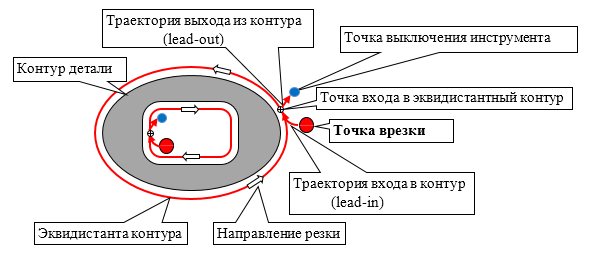
\includegraphics[width=0.9\textwidth]{cutting-path.png}
  \caption{Схема стандартной техники резки (резка по замкнутому контуру)}
  \label{standard-cutting}
  \end{center}
\end{figure}

Если используется стандартная техника резки,
то в этом случае каждый замкнутый контур вырезается целиком,
и после резки одного контура переход к следующей точке врезки
происходит с выключенным инструментом на холостом ходу.
При этом точка выключения инструмента
в общем случае
может не совпадать с точкой входа в эквидистантный контур заготовки,
по которому осуществляется резка, и также,
как и точка врезки,
может лежать вне заданного эквидистантного контура.
Во многих случаях допускается программирование точки выключения
инструмента непосредственно на эквидистантном контуре.

Стратегия минимизации тепловых деформаций при термической резке
и требования к качеству реза порождают необходимость управления
не только выбором точек врезки,
но и управлением траекторией подхода к контуру
(\textit{lead-in})
и способом выхода из контура
(\textit{lead-out}).
В зависимости от конкретных условий
(вида термической резки, марки и толщины материала,
скорости резки, геометрической формы контура и пр.)
подход к контуру может осуществляться по дуге окружности,
касательная к которой совпадает с касательной к контуру в точке входа,
либо производиться по прямой линии
(например, по наикратчайшему расстоянию до контура).
Соответственно и после завершения резки выход из контура
также может осуществляться с включенным инструментом
(либо по дуге, либо по прямой линии).
Необходимость выхода из контура с включенным
инструментом может быть вызвана тем,
что в точке выключения инструмента может возникнуть
<<вырыв>> или оплавление части материала,
что приводит к искажению геометрии заготовки.
Уменьшение эффекта деформации заготовок обеспечивает
также врезка в <<угловые>> точки заготовок
(рис.~\ref{corner}).

\begin{figure}[h]
  \begin{center}
  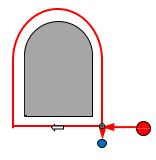
\includegraphics[width=0.3\textwidth]{corner.png}
  \caption{Пример врезки <<в угол>>}
  \label{corner}
  \end{center}
\end{figure}

Примером нестандартной техники
может служить <<цепная>> резка,
которая заключается в резке нескольких контуров с
использованием одной точки врезки.
При этом каждый контур,
как и в случае применения стандартной техники резки,
вырезается целиком.
На рис.~\ref{chain}
показан пример схемы резки двух заготовок,
в которой резка внешних контуров обеих заготовок
производится без выключения инструмента
с использованием только одной точки врезки.

Перемещение инструмента в точку врезки
в этом примере начинается из начальной точки на холостом ходу,
а после завершения резки последнего контура
предусмотрен возврат инструмента в начальную точку.

\begin{figure}[h]
  \begin{center}
  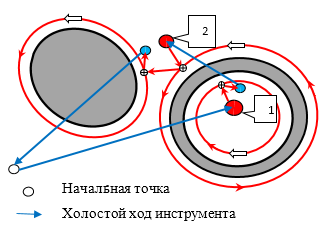
\includegraphics[width=0.5\textwidth]{chain.png}
  \caption{Пример схемы резки двух заготовок с использованием стандартной и <<цепной>> техники резки}
  \label{chain}
  \end{center}
\end{figure}

На практике применяется также техника резки
замкнутого контура заготовок по частям
с использованием нескольких точек врезки
с целью формирования т. н. <<перемычек>>
(рис.~\ref{jumper}),
а также используются другие специальные приемы,
целью которых является оптимизация различных параметров,
характеризующих процесс резки,
и соблюдение необходимых технологических требований резки.
Техника резки <<перемычка>> предусматривает
оставление невырезанной части контура заготовки,
обычно небольшого прямолинейного отрезка или нескольких отрезков
с резкой этих отрезков после завершения резки оставшейся части контура.
Этот прием применяется с целью уменьшения деформаций материала
при термической резке заготовок, склонных к термическим деформациям,
в частности, длинномерных заготовок.

\begin{figure}[h]
  \begin{center}
  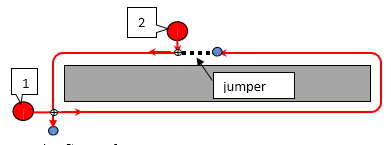
\includegraphics[width=0.5\textwidth]{jumper.png}
  \caption{Схема формирования перемычки на контуре при резке полосы}
  \label{jumper}
  \end{center}
\end{figure}

На рис.~\ref{saber} показан пример искажения геометрической формы
(получения т. н. формы <<сабли>>)
и~изменения размера длинномерной прямоугольной заготовки,
вырезаемой без использования техники <<перемычка>>.

\begin{figure}[h]
  \begin{center}
  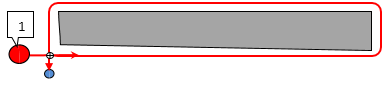
\includegraphics[width=0.5\textwidth]{saber.png}
  \caption{Результат изменнения формы и размера прямоугольной заготовки при термической резке}
  \label{saber}
  \end{center}
\end{figure}

На рис.~\ref{bridge}
приведен пример использования техники <<мост>>,
предполагающей  частичную резку замкнутого контура
заготовки с последующим завершением резки контура
после резки контура другой заготовки или
группы контуров других заготовок.
Эта техника используется при резке двух или
нескольких рядом расположенных заготовок и
предусматривает переход по короткой траектории (<<мосту>>)
к резке другой заготовки и возврат к первому контуру
по этой же траектории для завершения процесса резки.
Так же, как и <<перемычки>>,
мосты существенно уменьшают тепловые деформации материала,
особенно при резке длинномерных заготовок,
кроме того, сокращают число точек врезки.

\begin{figure}[h]
  \begin{center}
  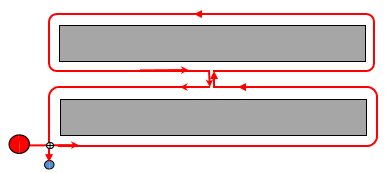
\includegraphics[width=0.5\textwidth]{bridge.png}
  \caption{Схема резки двух полос с использованием техники <<мост>>}
  \label{bridge}
  \end{center}
\end{figure}

Разновидностью техники <<мост>> можно считать технику <<змейка>>
(рис.~\ref{snake}),
в которой также используется прием
частичной резки контура и резки
нескольких заготовок без выключения инструмента.

\begin{figure}[h]
  \begin{center}
  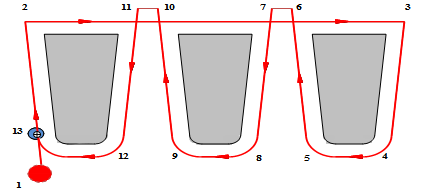
\includegraphics[width=0.7\textwidth]{snake.png}
  \caption{Схема резки <<змейка>>}
  \label{snake}
  \end{center}
\end{figure}

Для уменьшения длины рабочего хода инструмента
применяют т. н. <<совмещенный>> рез.
Он используется для вырезки заготовок,
которые содержат прямолинейные отрезки в контуре
и которые в процессе раскроя размещаются таким образом,
что имеют общую границу по одному из таких прямолинейных отрезков.
Общая прямолинейная граница позволяет размещать
заготовки с половинным припуском на рез
(т. е. на ширину реза),
поскольку режется только один раз,
что экономит материал и сокращает суммарную
длину резки на величину совмещенного реза.
Совмещенный рез реализован, в частности,
в технике резки <<восьмерка>>,
применяемой для резки двух одинаковых заготовок
(рис.~\ref{8}).
В этой технике используется также идея цепной резки.

\begin{figure}[h]
  \begin{center}
  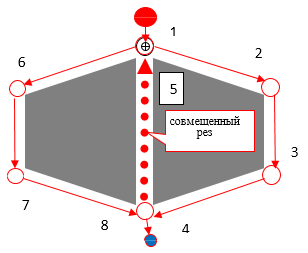
\includegraphics[width=0.6\textwidth]{8.png}
  \caption{Схема резки <<восьмеркой>> двух заготовок}
  \label{8}
  \end{center}
\end{figure}

Основные технологические требования
фигурной резки на машинах с ЧПУ обусловлены
необходимостью учета возникающих деформаций
материала и искажения геометрических размеров
вырезаемых заготовок при использовании
термических технологий резки.
Применение специальных техник позволяет
уменьшить эффект искажения геометрии,
который особенно значителен при
использовании газовой и плазменной технологий.

При использовании любой техники резки маршрут инструмента
машины с ЧПУ для фигурной листовой резки
включает в себя следующие компоненты:
\begin{itemize}
  \item точки врезки;
  \item рабочий ход инструмента;
  \item точки выключения инструмента;
  \item линейное перемещение инструмента на холостом ходу
  между точкой выключения инструмента и следующей точкой врезки.
\end{itemize}

При разработке управляющей программы
первое перемещение инструмента обычно
программируется, как на рис.~\ref{chain},
из начальной точки.

Отметим, что некоторые машины фигурной листовой
резки с ЧПУ могут быть укомплектованы
специальным видом инструмента,
т. н. трехрезаковым блоком для вырезания
из листа заготовок с одновременной разделкой
кромок поверхности реза для последующей сварки.
Врезка в материал для такого инструмента
программируется специальными способами.

Введем некоторые определения,
касающиеся понятия маршрута резки.
В дальнейшем при формальном обозначении
математических и геометрических категорий
мы будем использовать стандартную
теоретико-множественную символику.
Ее детальное описание дано в разделе 3.1.
%%% TODO! Fix reference ^^^^^^^^^^^^^^
Введем следующее определение.

\begin{opred}
\label{Opred1}
{\bf Сегментом резки}
$S=MM^*$
будем называть траекторию рабочего хода
инструмента между точкой врезки
$M$
и соответствующей ей точкой выключения инструмента
$M^*$.
Геометрически сегмент резки представляет собой
определенную на эвклидовой плоскости
$\mathbb R \times \mathbb R$
кривую.
$(S \subset \mathbb R \times \mathbb R;
M=(x,y) \in \mathbb R \times \mathbb R,
M^* =(x^*,y^*)\in \mathbb R \times \mathbb R)$.
Будем также полагать,
что в каждой точке траектории определено направление движения инструмента.
Заметим, что если сегмент резки не содержит замкнутых контуров,
то направление движения резки в каждой точке траектории
однозначно определяется начальной точкой сегмента
(точкой врезки).
Замкнутые контуры в траектории рабочего хода инструмента
могут появляться не только в результате резки контуров заготовок,
но и при программировании т. н. петель,
которые используются для повышения качества реза.
\end{opred}

Используя понятие сегмента резки,
все техники фигурной резки на машинах с ЧПУ
можно разделить на три класса.
\begin{enumerate}
  \item
  {\it Резка по замкнутому контуру (стандартная техника)}:
  в этом случае сегмент резки содержит
  ровно один замкнутый эквидистантный контур заготовки,
  который вырезается целиком.
  \item
  {\it Мультисегментная резка контура}:
  в этом случае для вырезки одного контура
  используются не менее двух сегментов резки.
  \item
  {\it Мультиконтурная резка}:
  резка предполагает вырезку нескольких
  контуров в одном сегменте.
\end{enumerate}

Примерами мультиконтурной резки являются,
в частности, приведенные выше техники резки:
<<цепная резка>>, <<мост>>, <<змейка>> и <<восьмерка>>,
а примером мультисегментной резки --
резка с перемычкой.
На практике используются и другие специальные техники резки,
но все они являются разновидностями техник,
относящихся к одному из определенных выше классов.

При разработке управляющих программ для
машин фигурной листовой резки с ЧПУ чаще всего
применяется стандартная техника резки.
Вместе с тем нередко используются и
комбинации различных техник резки.
Применение той или иной техники резки
при проектировании маршрута резки в
каждом конкретном случае, как правило,
обусловлено либо технологическими требованиями резки,
либо стремлением оптимизировать некоторые
параметры листовой резки.
Подробнее эти вопросы рассмотрены ниже.

\section{Маршрут резки и оптимизационные задачи маршрутизации инструмента машин листовой резки с ЧПУ}

Для формального определения маршрута резки
введем следующие обозначения.
Пусть
$A_1, A_2, \dots A_n$
– двумерные геометрические объекты (точечные замкнутые множества),
представляющие собой односвязные или
многосвязные области эвклидовой плоскости
$\mathbb R \times \mathbb R$,
ограниченные одной или несколькими замкнутыми кривыми
(граничными контурами)
$C_1, C_2, \dots C_N$
$(A_i, C_J \subset \mathbb R \times \mathbb R;
i \in \overline{1,n};
j \in \overline{1, N};
N \geqslant n)$.
Объекты
$A_1, A_2, \dots A_n$
являются геометрическими моделями плоских заготовок/деталей
({\it в дальнейшем в книге термин <<деталь>>,
которая вырезается из листового материала,
будет использоваться как синоним термина <<заготовка>>}).

Пусть также определена область размещения объектов
$B \subset \mathbb R \times \mathbb R$,
которая является геометрической моделью листового материала,
из которого вырезаются детали.
В общем случае область размещения
может содержать несколько кусков материала
(не обязательно прямоугольной формы),
но для решения оптимизационных задач
маршрутизации инструмента целесообразно рассматривать
в качестве области размещения одно замкнутое точечное множество,
ограниченное (как и деталь)
одним внешним контуром.
При этом допустимо наличие отверстий в материале
(внутренних контуров).
Будем полагать, что зафиксирован некоторый вариант размещения
объектов в области размещения,
при этом выполнены условия взаимного непересечения объектов.
Полагаем также, что выполнены другие дополнительные условия,
обусловленные технологические требованиями резки деталей
на конкретном технологическом оборудовании с ЧПУ,
в частности, условие соблюдения необходимой ширины реза.
Другими словами, фиксированный вариант размещения объектов
является допустимым вариантом раскроя листового материала
для заданного набора $n$ деталей.

Пример размещения в прямоугольной области 24 объектов
($n=24$),
описываемых 30 замкнутыми контурами
($N=30$)
с заданным минимальным расстоянием между объектами,
приведен на Рис. \ref{nesting}.
Раскройная карта получена с
помощью подсистемы автоматического раскроя CAD/CAM системы <<Сириус>>.

\begin{figure}
  \begin{center}
  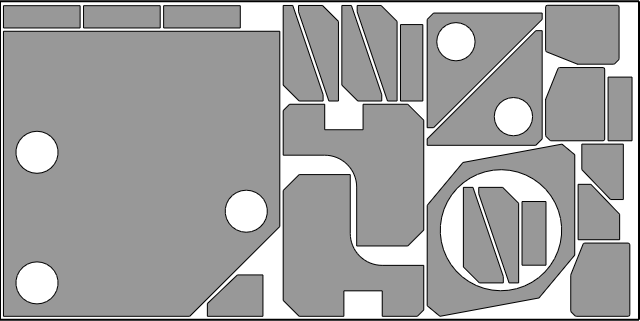
\includegraphics[width=0.9\textwidth]{nesting.png}
  \caption{Пример раскроя листа $2000 \times 1000$ мм с заданным минимальным расстоянием между деталями 10 мм}
  \label{nesting}
  \end{center}
\end{figure}

Предположим, что для вырезки деталей было использовано
$K$
сегментов резки
$S_k=M_kM^*_k; k \in \overline{1,K}$.
Тогда маршрут резки деталей можно определить
в терминах сегментов резки как кортеж

\begin{equation}
  ROUTE = (
    M_0, M_1, S_1, M_1^*, M_2, S_2, M_2^*, \dots M_K, S_K, M_K^*, i_1, i_2, \dots i_K
  )
  \label{tuple}
\end{equation}
где
$i_1, i_2, \dots i_K$
– последовательность, в которой вырезаются используемые сегменты резки
$S_1, S_2, \dots S_K$,
$M_0$
– начальная точка положения инструмента.
Линейное перемещение инструмента на холостом ходу
между точкой выключения инструмента и следующей точкой врезки
однозначно определяется этой последовательностью.
Если применить комбинаторную терминологию,
то последовательность однозначно задается перестановкой порядка
$K$,
т.е. упорядоченным набором натуральных чисел от $1$ до $K$
(биекцией на множестве $\overline{1,K}$),
которая числу
$k \in \overline{1,K}$
ставит в соответствие элемент
$i_k$ из набора.
Отметим, что термин <<маршрут резки>> является
общепринятым технологическим понятием.
В главах 3-5 при описании математических моделей оптимизации
маршрута резки мы будем использовать термин <<маршрут>>
применительно к перестановке
$i_1, i_2, \dots i_K$,
что, в свою очередь, соответствует устоявшейся
терминологии в задаче о последовательном обходе мегаполисов.

\begin{figure}
  \begin{center}
  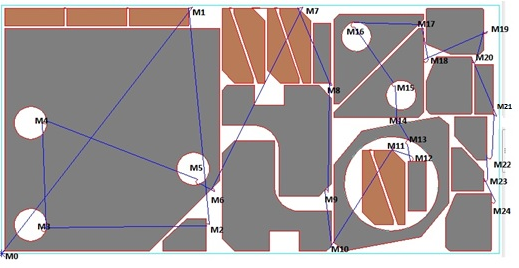
\includegraphics[width=0.9\textwidth]{cutting.png}
  \caption{Пример маршрута резки, содержащего 24 сегмента резки}
  \label{cutting}
  \end{center}
\end{figure}

На рис. \ref{cutting}
показана схема одного из возможных маршрутов резки для примера,
приведенного на Рис. \ref{nesting}.
Маршрут резки содержит 24 сегмента.
Для резки внешних контуров трех групп деталей
с точками врезки $M_1$
(три детали в группе),
$M_7$
(четыре детали в группе) и
$M_{11}$
была использована мультиконтурная резка
(указанные группы деталей выделены коричневым цветом).
Все остальные контуры вырезаны с применением стандартной техники резки.
Последовательность резки сегментов соответствует
номерам точек врезки $M_J$ ($J=1,2,\dots 24$).
После вырезки последнего сегмента
возврат инструмента в начальную точку $M_0$
не программировался.

На приведенном рисунке визуализация траектории инструмента
осуществляется точно по граничным контурам деталей,
а не по их эквидистантным контурам, хотя,
как отмечено выше,
траектория реза должна отстоять от
граничного контура на половину ширины реза.
Это связано с тем, что в большинстве CAM – систем
программирование движения инструмента первоначально
осуществляется по граничным контурам деталей,
а вычисление реальной траектории производится
либо непосредственно самой системой ЧПУ,
либо специальной программой-постпроцессором,
предназначенной для конвертирования информации о
маршруте резки из внутреннего формата системы в
формат команд конкретного технологического оборудования с ЧПУ.
В первом случае величину припуска на рез
устанавливает оператор на станке перед запуском
управляющей программы резки.

В дальнейшем без ограничения общности мы будем полагать,
что траектория инструмента в маршруте резки $ROUTE$
программируется по граничным контурам,
и сегменты резки
$S_k=M_kM^*_k; k \in \overline{1,K}$
содержат все граничные контуры деталей
$C_1, C_2, \dots C_N$,
т.е.
$$
\bigcup_{j=1}^N C_j \subset \bigcup_{k=1}^K S_k
$$
Соответственно, все точки входа в эквидистантный контур
(и выхода из эквидистантного контура)
(см. Рис. \ref{standard-cutting})
также лежат на граничных контурах.

На рис. \ref{control-program} показан фрагмент управляющей программы
(G-кода) для машины листовой газовой резки
типа <<Комета>> с системой ЧПУ 2Р32М.

\begin{figure}
\begin{multicols}{3}

  \%УП\_2Р32М\_01
  N1G91 \\
  N2G00X7662Y9909F6000 \\
  N3M70T1 \\
  N4M71T1 \\
  N5G01X-141Y-48F460 \\
  N6X-2400  \\
  N7X-40  \\
  N8X-67  \\
  N9X-2400  \\
  N10X-40 \\
  N11X-67 \\
  N12X-2400 \\
  N13Y-700  \\
  N14X2400  \\
  N15Y700 \\
  N16Y40  \\
  N17X107Y-40 \\
  N18Y-700  \\
  N19X2400  \\
  N20Y700 \\
  N21Y40  \\
  N22X107Y-40 \\
  N23Y-700  \\
  N24X2400  \\
  N25Y700 \\
  N26Y40  \\
  N27M74T1  \\
  N28G00X817Y-8745F6000 \\
  N29M71T1  \\
  N30G03X-108Y0I-54J0F460 \\
  N31G01Y-1048  \\
  N32X-1740 \\
  N33Y400 \\
  N34X940Y900 \\
  N35X800 \\
  N36Y-252  \\
  N37X20Y-30  \\
  … \\
  N314M71T1 \\
  N315G02X-130Y0I-65J0F460  \\
  N316G01Y267 \\
  N317G03X-50Y50I-50J0  \\
  N318G01X-1366 \\
  N319G03X-46Y-31I0J-50 \\
  N320G01X-384Y-960 \\
  N321G03X-4Y-19I46J-19 \\
  N322G01Y-1120 \\
  N323G03X14Y-35I50J0 \\
  N324G01X122Y-121  \\
  N325G03X37Y-14I35J35  \\
  N326G01X1627Y-1 \\
  N327G03X50Y50I0J50  \\
  N328G01Y1933  \\
  N329X20Y30  \\
  N330M74T1 \\
  N331M75T1 \\
  N332M02 \\
  M30
\end{multicols}
\caption{Фрагмент УП для машины листовой резки <<Комета>> с ЧПУ 2Р32М }
\label{control-program}
\end{figure}

Программа сгенерирована на основе маршрута резки
(спроектированного в интерактивном режиме в CAD/CAM системе <<Сириус>>
и показанного на Рис. \ref{cutting})
соответствующим постпроцессором со
следующими числовыми параметрами резки:
\begin{itemize}
  \item	Число строк в УП – 333;
  \item	Количество точек врезки (пробивки листа) – 24;
  \item	Путь инструмента на рабочей скорости – 27.36 метров;
  \item	Путь инструмента на быстром (холостом) ходу – 8.39 метров;
  \item	Время движения на рабочей скорости – 62.04 мин.;
  \item	Время движения на быстром (холостом) ходу – 1.64 мин.;
  \item	Общее время резки: 63.68 мин.
\end{itemize}

В зависимости от выбранного маршрута резки,
числовые параметры резки могут существенно различаться.
Таким образом, при разработке управляющих программ
для машин фигурной листовой резки с ЧПУ возникают
различные задачи оптимизации маршрута инструмента.
В качестве критерия оптимизации (целевой функции)
в этих задачах чаще всего рассматривается общее время резки.
При термической и гидроабразивной резке для сформированного
маршрута резки общее время резки
$T_{cut}$
рассчитывается по следующей формуле:
\begin{equation}
  T_{cut} = \frac{L_{on}}{V_{on}} + \frac{L_{off}}{V_{off}} +N_{pt} \cdot t_{pt}
  \label{cutting-time}
\end{equation}
где
$L_{off}$ – длина переходов с выключенным режущим инструментом (холостой ход);
$L_{on}$ – длина реза с включенным режущим инструментом;
$V_{off}$ – скорость холостого хода;
$V_{on}$ – скорость рабочего хода режущего инструмента;
$N_{pt}$ – количество точек врезки;
$t_{pt}$ – время, затрачиваемое на одну точку врезки.
При этом подразумевается,
что получаемое в результате врезки отверстие
расположено внутри материала листа.
Однако при резке заготовок, как отмечалось,
могут быть использованы и другие типы врезки,
что приводит к изменению времени врезки
$t_{pt}$
в этих случаях.
Если при резке деталей было использовано несколько типов врезки,
то формула (\ref{cutting-time}) запишется в более общем виде:
\begin{equation}
  T_{cut} = \frac{L_{on}}{V_{on}} + \frac{L_{off}}{V_{off}} +
  \sum_{j=1}^p N_{pt}^j \cdot t_{pt}^j
  \label{cutting-time-multi}
\end{equation}
где
$p$ - число использованных типов врезки,
$N_{pt}^j$ – количество точек врезки типа j;
$t_{pt}^j$ – время, затрачиваемое на одну точку врезки типа j.
И в (\ref{cutting-time}), и в (\ref{cutting-time-multi})
значение скорости холостого хода инструмента
$V_{off}$ – константа,
определяемая техническими характеристиками
используемого технологического оборудования.
Значение скорости рабочего хода инструмента
$V_{on}$
программируется при разработке управляющей программы
в соответствии с используемой технологией резки
и параметрами листового материала
(марка материала и толщина).
Предполагается, что заданная величина
$V_{on}$  в (\ref{cutting-time}) и в (\ref{cutting-time-multi})
также является константой,
однако на практике фактическая скорость резки
может меняться в зависимости от различных технологических факторов,
а также характеристик спроектированной управляющей программы.
Это диктует необходимость проведения исследований для
определения поправочного коэффициента для величины
$V_{on}$.
В \S 1.4
%%% TODO ^^^^^^^^^^^^^ fix reference
будут приведены результаты такого рода исследований
применительно к машине лазерной резки с ЧПУ
ByStar 3015 для листового материала АМг3М толщиной от 1,5 до 5 мм.

Важнейшей экономической характеристикой качества
разработанной управляющей программы является стоимость
(себестоимость) резки деталей на машине с ЧПУ.
Это сложный интегрированный показатель,
который включает в себя произведенные во время
резки затраты на электроэнергию и расходные материалы,
на обслуживание машины с ЧПУ,
а также другие эксплуатационные затраты.
Отметим, что стоимость резки не всегда
пропорциональна времени резки,
поскольку зависит еще и от различных режимов резки.
По аналогии с формулой времени резки (\ref{cutting-time})
показатель стоимости резки можно определить по следующей формуле:
\begin{equation}
  F_{cost}=
  L_{on} \cdot C_{on} +
  L_{off} \cdot C_{off} +
  N_{pt} \cdot C_{pt}
  \label{cutting-cost}
\end{equation}
где
$C_{on}$ – стоимость единицы пути с включенным режущим инструментом;
$C_{off}$ – стоимость единицы пути с выключенным режущим инструментом;
$C_{pt}$ – стоимость одной точки врезки,
а $L_{on}, L_{off}, N_{pt}$
имеют тот же смысл, что и в формуле (\ref{cutting-time}).
При этом $C_{on}, C_{off}, C_{pt}$
– величины, зависящие от типа машины с ЧПУ,
технологии резки, используемой скорости рабочего хода инструмента,
толщины и марки материала.
Функциональная зависимость
$C_{on}, C_{off}, C_{pt}$
от перечисленных параметров
может задаваться либо табличными функциями,
либо аналитически.
При этом абсолютные значения этих величин
на российских предприятиях, использующих машины с ЧПУ,
определяются экономическими службами с учетом многих факторов,
и могут существенно различаться на разных предприятиях.
Зачастую стоимость резки вообще не учитывается
в раскройно-заготовительном производстве,
либо рассчитывается на основании специальных нормативов,
не зависящих от величин
$L_{on}, L_{off}, N_{pt}$.

Очевидно, что необходимость расчета стоимости резки
для каждой управляющей программы резки возникает на предприятиях,
оказывающих услуги сторонним организациям по резке материала.
Однако и на многих таких предприятиях для определения
стоимости резки учитывается только длина рабочего хода инструмента
$L_{on}$,
которая принимается равной суммарному периметру граничных контуров вырезаемых деталей
$C_1, C_2, \dots c_N$,
что, естественно, приводит к неадекватной оценке эффективности процесса резки.
В дальнейшем при оптимизации стоимостных параметров резки
мы будем применять теоретически обоснованный способ определения
показателя стоимости резки, задаваемый формулой (\ref{cutting-cost}).
На рис. \ref{cost} представлен расчет стоимости резки
$F_{cost}$
для рассматриваемого примера при резке деталей на машине газовой резки.
Значения величин
$C_{on}, C_{off}, C_{pt}$
взяты из таблицы, используемой для расчета себестоимости фигурной
листовой резки на одном из предприятий Свердловской области.

\begin{figure}
  \begin{center}
  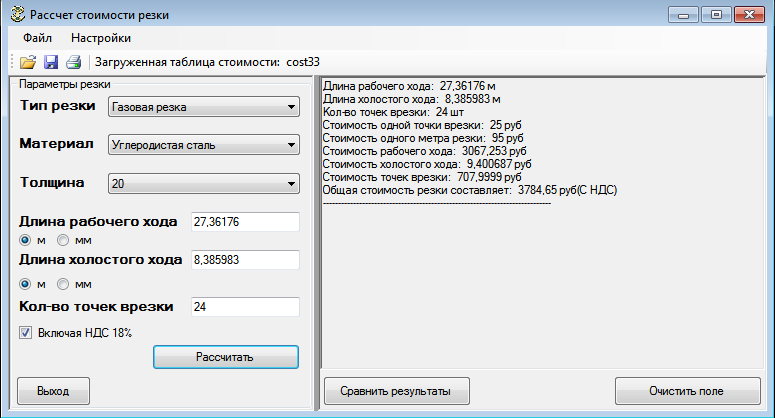
\includegraphics[width=0.9\textwidth]{cost.png}
  \caption{Пример расчета стоимости резки $F_{cost}$ при резке деталей из углеродистой стали толщины 20 мм на машине газовой резки}
  \label{cost}
  \end{center}
\end{figure}

Следует отметить,
что задача правильного определения величин
$C_{on}$, $C_{off}$, $C_{pt}$
для конкретного технологического оборудования
и конкретного материала сама по себе является малоисследованной проблемой.
В \S 1.4
%%% TODO ^^^^^^^^^^^^^ fix reference
будут приведены результаты исследования,
позволяющего точно вычислять себестоимость
лазерной резки применительно для машины с ЧПУ
ByStar3015 при резке углеродистой и нержавеющей
стали различных толщин
(на примере Ст10кп и 12Х18Н10Т),
а также при резке алюминия и его сплавов (на примере Амг3М).

В случае использования нескольких типов врезки формула (\ref{cutting-cost}) примет вид:
\begin{equation}
  F_{cost}=
  L_{on} \cdot C_{on} +
  L_{off} \cdot C_{off} +
  \sum_{j=1}^p N_{pt}^j \cdot C_{pt}^j
  \label{cutting-cost-multi}
\end{equation}
где $C_{pt}^j$ - стоимость одной точки врезки типа $j$.

Как легко заметить,
значения целевых функций (\ref{cutting-time}) – (\ref{cutting-cost-multi})
однозначно определяются маршрутом резки, задаваемым кортежем (\ref{tuple}),
поскольку геометрия сегментов резки
$S_1, S_2, \dots S_K$
позволяет вычислить длину рабочего хода инструмента  $L_{on}$,
а координаты точек
$M_0$, $M_1$, $M_1^*$, $M_2$, $M_2^*$ ... $M_K$, $M_K^*$
и перестановка
$i_1$, $i_2$, ... $i_K$
(последовательность, в которой вырезаются используемые сегменты резки),
задают набор холостых перемещений инструмента,
который определяет суммарную длину холостого хода  $L_{off}$.

Таким образом, сформулированные задачи оптимизации
маршрута инструмента для машин фигурной листовой резки с ЧПУ
можно представить в самом общем виде
как задачу минимизации некоторой числовой функции $F$,
заданной на множестве $G$ допустимых кортежей $ROUTE$, т.е.
\begin{equation}
  F(ROUTE) \to \min_{ROUTE \in G}
  \label{problem-statement}
\end{equation}

Поскольку элементы кортежа содержат
(помимо последовательности резки
$i_1, i_2, \dots i_K$,
выбираемой из дискретного множества перестановок)
точки врезки и точки выключения инструмента
$M_kM_k^*, k \in \overline{1,K}$,
которые, в свою очередь,
могут быть выбраны из континуальных подмножеств евклидовой плоскости
$\mathbb R \times \mathbb R$,
даже в случае наложения существенных ограничений
на возможность выбора допустимых сегментов
$S_k$
оптимизационная задача (\ref{problem-statement})
может быть отнесена к классу очень сложных задач
непрерывно-дискретной оптимизации.
Некоторые вопросы формирования допустимых сегментов резки мы рассмотрим в части 2
настоящей монографии при математической формализации задачи (\ref{problem-statement})
и ее сведении к задаче о последовательном обходе мегаполисов.
В следующем параграфе мы сформулируем основные ограничения
на допустимые значения элементов последовательности резки
$i_1, i_2, \dots i_K$
и на значения
$M_kM_k^*, k \in \overline{1,K}$,
вызванные особенностями технологии листовой резки на машинах с ЧПУ.

%!!! Проверить в финальном варианте !!!
%\newpage
\section{Технологические ограничения на параметры маршрута инструмента машин листовой резки с ЧПУ}
\subsection{Ограничения на координаты точек врезки и точек выключения инструмента, обусловленные деформацией материала при врезке}
Этот тип ограничений связан с тем,
что для соблюдения технологии врезки любая точка врезки
$M_k$
должна лежать (как отмечалось выше)
на некотором ненулевом расстоянии от контура детали,
по которому движется инструмент.
При этом координаты точки врезки должны,
естественно, находиться вне областей,
занимаемых геометрическими образами других деталей с учетом припуска на рез.
Величины необходимых минимально допустимых расстояний
от контуров детали до точек врезки и точек выключения
инструмента определяются различными технологическими параметрами.
Другими словами, этот тип ограничений носит геометрический характер
и определяет геометрические области на раскройной карте,
в которых допустимо задавать точки врезки для формирования сегментов резки.

Для общей формализации этих ограничений обозначим через
$E_j^d$ – эквидистанты замкнутых контуров $C_j$,
удаленные от них на величину $d$,
а через
$P_j^d$ – двумерные геометрические объекты (замкнутые точечные множества),
ограниченные этими эквидистантами
$E_j^d = \partial P_j^d$,
$P_j^d \subset \mathbb R \times \mathbb R$.
При этом будем полагать,
что для внешних контуров деталей
$E_j^d$
является внешней эквидистантой,
а для внутренних – внутренней.
Пусть $ОUT$ - конечное множество индексов внешних контуров деталей,
а $IN$ – соответственно множество индексов внутренних контуров.
Обозначим  размерность этих множеств соответственно $l$ и $s$,
т.е.
$OUT = \{j_1, j_2, \dots j_l\};
IN = \{q_1, q_2, \dots q_s\}$
$(OUT  \subseteq \overline{1,N};
IN  \subset \overline{1,N})$.
Заметим, что если $l=N$
(все контуры являются внешними), то
$IN = \varnothing$
$(s = 0)$.
Пусть $d1$ – минимально допустимое расстояние от контуров деталей до точек врезки,
тогда выбранные точки врезки для каждого сегмента резки должны удовлетворять следующим условиям:
\begin{equation}
  \forall k \in \overline{1,K}:
  M_k \in G_M,
  \text{где}\:
  G_M = \big(B \setminus \bigcup_{j\in OUT} P_j^{d1} \big)
  \cup
  \big( \bigcup_{q\in IN}P_q^{d1} \big)
  \label{pierce-constraint}
\end{equation}

Как мы уже отмечали,
минимально допустимое расстояние от граничных контуров деталей
до точек врезки,
задаваемых на границе листа,
или подготовленных предварительно механическим способом,
может быть несколько меньше,
чем до точек врезки, получаемым стандартным <<прожиганием>> (пробивкой) материала листа.
Для таких особых точек врезки область $G_M$,
задаваемая условием (\ref{pierce-constraint}),
может быть расширена.
Это условие являются необходимым, но не достаточным,
и для конкретных задач могут возникать дополнительные ограничения,
обусловленные технологическими особенностями резки,
о которых пойдет речь ниже.
В этих случаях, наоборот, область $G_M$
может быть существенно сокращена.

Аналогичное условию (\ref{pierce-constraint})
ограничение справедливо и для точек выключения инструмента:
\begin{equation}
  \forall k \in \overline{1,K}:
  M_k^* \in G_{M^*},
  \text{где}\:
  G_{M^*} = \big(B \setminus \bigcup_{j\in OUT} P_j^{d2} \big)
	\cup
  \big( \bigcup_{q\in IN}P_q^{d2} \big)
  \label{tool-off-constraint}
\end{equation}
где $d2$ – минимально допустимое расстояние
от контуров деталей до точек выключения инструмента,
которое, чаще всего, меньше $d1$
и может, как отмечалось, быть и нулевым.

На Рис. \ref{pierce-area} указаны геометрические области листа,
допустимые для определения точек врезки при программировании резки
внешних граничных контуров деталей,
обозначенных на рисунке 1,2 и 3 и внутреннего граничного контура 4.
При этом минимально допустимое расстояние $d1$ от граничных контуров 1-4 до возможных точек врезки,
установленное пользователем CAM – системы, равно 9,5 мм.

\begin{figure}
  \begin{center}
  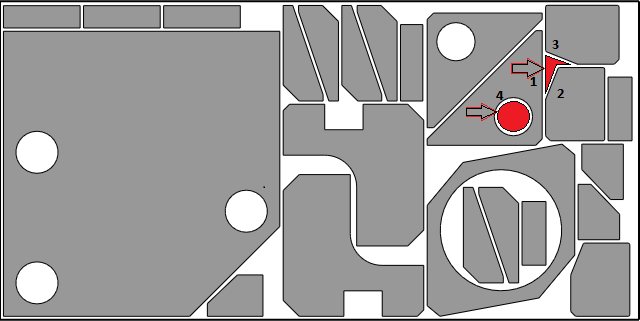
\includegraphics[width=0.9\textwidth]{pierce-area.png}
  \caption{Пример двух геометрических областей на раскройной карте (указаны стрелками),
допустимых для задания точек врезки }
  \label{pierce-area}
  \end{center}
\end{figure}

\subsection{Условия предшествования}

Это условие накладывает ограничения на порядок вырезки сегментов
$ I = (i_1, i_2, \dots i_K)$.
Ограничения на порядок их резки обусловлены особенностями
технологии и оборудования листовой резки с ЧПУ,
которые не позволяют после вырезки внешнего контура точно
позиционировать инструмент для вырезки внутренних контуров,
поскольку деталь после вырезки внешнего контура может
изменить свое положение на раскройном столе.
Это вызвано тем, что после вырезки внешнего контура
вырезанная деталь <<теряет>> связь с листом,
а для многих типов раскройных столов эта деталь
может даже изменить свое положение относительно плоскости листа
(упасть между статическими конструкциями раскройного стола).
При выборе последовательности контуров следует придерживаться следующих правил.

{\it Правило 1}.
Если внешний контур имеет один или более внутренних контуров,
которые представляют собой границы отверстий в деталях,
то прежде, чем будет начата вырезка внешнего контура,
должны быть вырезаны все внутренние контуры.

{\it Правило 2}.
Если внутренний контур детали на раскройной карте
содержит внешний контур/контуры другой детали,
то сначала должна быть вырезана эта другая деталь
с соблюдением {\it Правила 1}.

Перечисленные правила и называются условием предшествования для перестановки
$ I = (i_1, i_2, \dots i_K)$.
В терминах ее элементов условие означает следующее:
\begin{enumerate}
  \item
  если в перестановке
  $ I = (i_1, i_2, \dots i_K)$
  сегмент $i_k$
  содержит внешний контур,
  то все соответствующие внутренние контуры должны содержаться в сегментах,
  предшествующих сегменту $i_k$
  в перестановке;
  \item
  если в перестановке
  $ I = (i_1, i_2, \dots i_K)$
  сегмент $i_k$
  содержит  внутренний контур,
  который на раскройной карте содержит внутри внешний контур,
  соответствующий другому объекту
  $A_l$
  $(l=1,2, \dots n)$,
  то этот внешний контур должен быть вырезан в сегментах,
  предшествующих сегменту $i_k$ в перестановке $I$.
\end{enumerate}

Рис. \ref{precedence} иллюстрирует условие предшествования
при формировании маршрута резки для деталей,
содержащих внутренние контуры.

\begin{figure}
  \begin{center}
  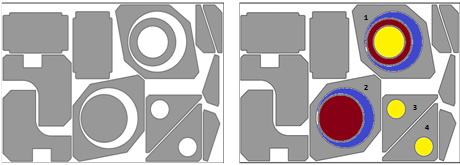
\includegraphics[width=0.9\textwidth]{precedence.png}
  \caption{Пример раскройной карты деталей, содержащих внутренние контуры}
  \label{precedence}
  \end{center}
\end{figure}

В соответствии с условиями предшествования резка контуров,
ограничивающих цветные области для 4-х деталей на Рис. \ref{precedence},
должна осуществляться в следующей последовательности:

\begin{enumerate}
  \item желтый, красный, синий, серый;
  \item	красный, синий, серый;
  \item	желтый, серый;
  \item желтый, серый.
\end{enumerate}

Условия предшествования и ограничения на координаты точек врезки
и точки выключения инструмента,
обусловленные деформацией материала при врезке,
имеют статический характер,
т.е. однозначно определяются спроектированной раскройной картой,
используемым для резки технологическим оборудованием
и свойством раскраиваемого материала.
В терминах маршрута резки $ROUTE$
и его параметров
$M_0$, $M_1$, $S_1$, $M_1^*$, $M_2$, $S_2$, $M_2^*$,... $M_K$, $S_K$, $M_K^*$,
$i_1$, $i_2$,... $i_K$
технологическое ограничение
1) однозначно определяет допустимые геометрические области
$G_M$
и
$G_{M^*}$
для выбора точек врезки и точек выключения инструмента,
а технологическое ограничение
2) накладывает запрет на некоторые значения перестановки
$ I = (i_1, i_2, \dots i_K)$
при формировании порядка резки сегментов. При
этом сформулированные требования не зависят от задаваемых параметров кортежа
$ROUTE$.

В отличие от этих двух технологических ограничений
следующий тип технологических требований устанавливает
дополнительные ограничения на выбор точки врезки и выбор
порядка резки сегментов на каждом шаге формирования маршрута резки
(т.е. при определении параметров очередного выбираемого сегмента)
в зависимости от того какие параметры маршрута резки были выбраны на предыдущих шагах.
Этот тип ограничений обусловлен геометрическими
искажениями материала при термической резке деталей.

\subsection{Эвристические правила термической резки заготовок из листовых материалов}
\label{Par133}

Термические воздействия на вырезаемые заготовки можно подразделить на два типа\footnote{
  Сформулированные в \ref{Par133})
  правила разработаны сотрудниками ОАО <<Уралхиммаш>>
  В.И.Кротовым и А.Д.Гуртовенко на основе опыта
  резки листовых материалов на машинах термической резки с ЧПУ
  в котельно-заготовительном комплексе предприятия в 1992г
}:

\begin{itemize}
\item общие изменения геометрических размеров заготовки (уменьшение)
вследствие ее вырезания из нагретой части материала;
\item	изменение геометрической формы заготовок
(изменение радиусов у секторов,
отклонения от прямолинейности у прямоугольных деталей) и др.
Чем больше геометрические размеры заготовки,
тем больше изменения.
Наиболее  подвержены данным изменениям узкие длинные заготовки.
\end{itemize}

В Таблице \ref{thermal-classification}
приведена типология некоторых видов заготовок
по признаку подверженности термическим деформациям.
В качестве основных геометрических характеристик
классификации заготовок использованы габаритные размеры заготовок
(A - габаритная длина, B - габаритная ширина).
Приведенные в таблице типы заготовок относятся,
в основном, к номенклатуре машиностроительных предприятий,
но широко используются также в раскройно-заготовительном производстве
других отраслей промышленности.

\begin{table}
  \caption{Классификация заготовок по признаку подверженности термических деформаций}
  \label{thermal-classification}
  \begin{tabular}{ p{0.3\textwidth} p{0.3\textwidth} p{0.3\textwidth} }
  \hline
  Термическая характеристика заготовки
    & Описание заготовки
    & Геометрические характеристики заготовки \\
  \hline
  Заготовки, подверженные термическим деформациям изгиба
    & Полосы, узкие обечайки, секторы
    &	$B<100 \text{мм}, A>5B$ $100<B<250, A>8B$ \\
  Заготовки, подверженные термическим деформациям изгиба и изменением длины
    & Длинномерные и узкие полосы и обечайки, длинномерные секторы больших радиусов ($R>200$ мм)
    & $B <100 \text{мм}, A>10B$ $100<B< 300, A>15B$ \\
  Заготовки, не подверженные термическим деформациям
    & Фланцы, заглушки, диски, косынки, ребра, стенки, широкие сегменты и обечайки
    & $A/B < 5$ \\
  Заготовки, подверженные оплавлению и загрязнению при резке
    & Малогабаритные косынки, планки, ребра
    & $ A, B <200 \text{мм}$ \\
  Заготовки, вырезаемые с большим удельным тепловыделением
    & Полосы, обечайки, секторы со скосами кромок под сварку
    & $ A>300 \text{мм}, B>150 \text{мм}$ \\
  \hline
  \end{tabular}
\end{table}

В зависимости от термических характеристик заготовок
и от требований к их точности выбирается оборудование,
способ и последовательность резки.
Например, величина удельного тепловыделения –
наибольшая при газокислородной резке,
поэтому имеет смысл тонкие листы из углеродистых и
низколегированных сталей резать плазменно-дуговым способом,
дающим попутно большой выигрыш в производительности.
Металлы, обладающие более высокой теплопроводностью
менее склонны к термическим деформациям.
Термообработка листового проката уменьшает
тепловые деформации материала и наоборот:
необработанный лист более склонен к термическим деформациям,
т.к. в нем присутствуют высокие внутренние  напряжения,
которые накладываются на усилия, возникающие от  нагрева при резке.

На величину термических деформаций оказывают влияние:
\begin{itemize}
\item	тип резки (газовая, плазменная, лазерная);
\item	марка материала (его теплопроводность);
\item	состояние поставки металла (наличие внутренних напряжений), его термообработка;
\item	толщина металла;
\item	выбор порядка резки заготовок;
\item	выбор точек врезки для каждого контура;
\item	направление обхода контура (по/против часовой стрелки).
\end{itemize}

При работе в интерактивном режиме в CAM системе
пользователь может сам определять контуры или их части
для формирования сегментов резки,
выбирать порядок резки сегментов и координаты точек врезки
в нужном месте посредством курсора <<мыши>>.
Автоматический режим предполагает наличие в CAM системе
соответствующего алгоритма определения маршрута резки $ROUTE$
с соблюдением необходимых технологических требований.
Сформулируем наиболее важные из технологических требований резки,
обусловленные наличием термических деформаций материала.
Прежде всего, введем понятия правил <<жесткости заготовки>> и <<жесткости материала>>.

{\bf Правило <<жесткости заготовки>> (<<жесткости детали>>).}
Правило <<жесткости заготовки/детали>> касается выбора точек врезки
$M_k, k \in \overline{1,K}$
в маршруте резки  $ROUTE$,
а также выбора направления резки контуров деталей.
Оно заключается в том, что при резке контура точка
врезки и направление резки контура выбираются таким образом,
чтобы сначала вырезались участки контура,
расположенные в непосредственной близости к границе материала,
либо к границе вырезанной области,
а завершение резки происходило по участку контура,
граничащего с <<жесткой>> (не вырезанной) частью области.

Поясним правило <<жесткости заготовки>> на примере.
На Рис. \ref{part-hardness}
показаны 3 заготовки и 9 выбранных возможных точек врезки.

Предположим, что мы начинаем резку с заготовки <<А>>
и выбираем одну из первых 4 точек врезки (1-4).
Точка 2 является недопустимой для врезки,
поскольку при завершении резки не остается
<<жесткого>> участка не вырезанной области в материале,
и заготовка (еще до завершения резки контура)
начнет перемещаться относительно материала.
Кроме этого, заготовка будет получать максимальное
нагревание из-за малой площади остатка в области завершения резки.
Все это, в конечном итоге,
приведет к искажению геометрических размеров заготовки.

\begin{figure}
  \begin{center}
  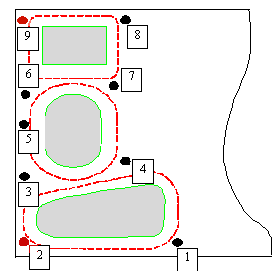
\includegraphics[width=0.5\textwidth]{part-hardness.png}
  \caption{Пример выбора точек врезки}
  \label{part-hardness}
  \end{center}
\end{figure}

Точки 1,3 и 4 являются допустимыми для врезки,
однако при выборе точки врезки 1 резка контура
должна производиться по часовой стрелке,
а при выборе точки 3 - против.
Для точки 4 – направление реза не является существенным.
При резке следующей заготовки (<<Б>>)
допустимы точки врезки 4,6 или 7.
Для точки 4 правило <<жесткости заготовки>>
предполагает движение резака по часовой стрелке,
а для точки 6 – против часовой стрелки.

И, наконец, при резке заготовки <<В>>
допустимы точки врезки 7 или 8.
Выбор точки врезки 7 диктует необходимость
движения резака по часовой стрелке,
а в случае выбора точки 8 – против часовой стрелки.

Таким образом, правило <<жесткости заготовок>>
существенно ограничивает свободу выбора точек
врезки и направлений обхода контура.
В частности, для данного примера,
если все контуры вырезаются по часовой стрелке,
то набор точек врезки 1, 4, 7
является наиболее предпочтительным,
а если против часовой стрелки, то – 4, 7, 8
(или 4,6,8).
Понятно, что строгая формализация процедуры
выбора представляется затруднительной,
и остальные допустимые варианты также не приведут
к критическим изменениям в геометрии заготовок,
но интуитивно ясно, что предлагаемые 3 варианта
несколько уменьшат тепловые деформации по сравнению
с другими допустимыми вариантами.

Важно отметить,
что при изменении порядка вырезки заготовок
(например, в последовательности <<В>>, <<Б>>, <<А>>)
изменится и набор допустимых точек врезки и направлений реза.

Функция определения допустимых
(как с точки зрения геометрических характеристик,
так и с точки зрения технологических требований резки)
точек врезки является важнейшей функцией CAM – системы
при автоматическом режиме формирования УП.

{\bf Правило <<жесткости материала>> (<<жесткости листа>>).}
Это правило определяет допустимый порядок
(последовательность)
$i_1, i_2, \dots i_k$,
в которой вырезаются используемые сегменты резки
$S_1, S_2, \dots S_K$.
Фактически это правило включает в себя несколько эвристических правил.
Рис. \ref{list-hardness}
иллюстрирует 4 правила выбора стороны материала,
с которой следует начинать процесс термической резки.
Правило а) рекомендует начинать процесс резки с узкой стороны листа (материала).
Правила б), в) и г) уточняют,
какую из узких сторон выбрать.
Алгоритм выбора заключается в следующем.

\begin{enumerate}
  \item
  Сначала определяем,
  есть ли среди заготовок длинномерные детали
  (длинномерной деталью в соответствии с Таблицей \ref{thermal-classification}
  будем называть заготовки, у которых один из габаритов больше другого не менее,
  чем в 10 раз).
  Если эти заготовки расположены вблизи
  узкой границы материала,
  то процесс резки следует начинать с них
  (правило б),
  так как именно такого рода заготовки
  подвержены максимальным тепловым деформациям.
  \item
  Затем определяем,
  есть ли на материале крупный отход.
  При наличии такого отхода с одной из сторон,
  процесс резки следует начать с противоположной стороны,
  поскольку аккумулирующееся в материале в процессе резки
  тепло в конечной стадии резки должно быть
  несколько скомпенсировано <<жестким>> остатком
  (правило в).
  \item
  И, наконец,
  если на материале нет крупного отхода,
  резку следует начинать с той стороны,
  где суммарные тепловыделения от резки больше
  (больше мелких деталей, либо больше суммарный периметр реза)
  (правило г).
\end{enumerate}

\begin{figure}
  \begin{center}
  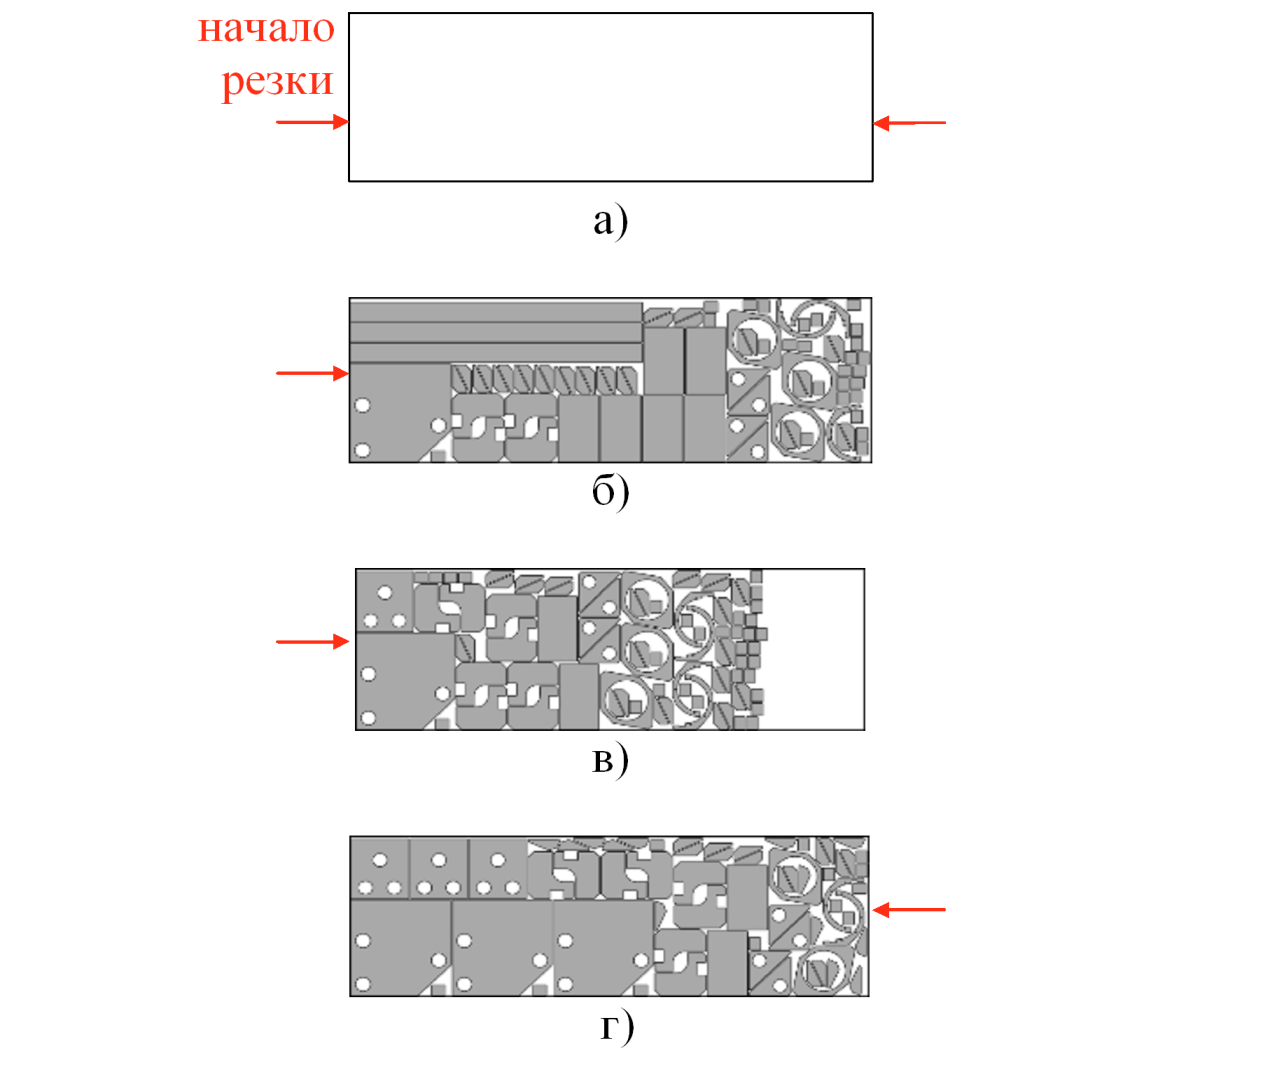
\includegraphics[width=0.9\textwidth]{list-hardness.png}
  \caption{Правила выбора начальной стороны материала }
  \label{list-hardness}
  \end{center}
\end{figure}

Еще два правила <<жесткости>> заключаются в том,
что при выборе последовательности вырезаемых заготовок
на материале не должно оставаться узких полос и <<островов>>,
содержащих не вырезанные заготовки
(см. Рис. \ref{island}).

\begin{figure}
  \begin{center}
  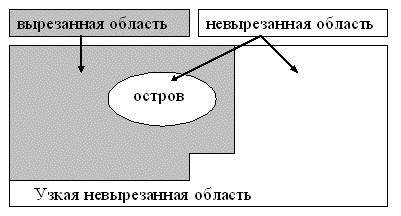
\includegraphics[width=0.6\textwidth]{island.png}
  \caption{Пример материала с недопустимыми не вырезанными областями}
  \label{island}
  \end{center}
\end{figure}

Для того чтобы обеспечить все правила <<жесткости материала>>,
следует предварительно разбить всю область резки на некоторые <<зоны>>
и затем процесс резки заготовок осуществлять
в этих зонах последовательно по возрастанию номеров зон,
т.е. область размещения $В$ разбивается на подобласти
\begin{equation}
  B_j = \bigcup_{r=1}^l \Omega_r
\end{equation}

где $l$
– количество выбранных зон для области $B$.
При этом формирование и нумерация зон
должна проводиться в соответствии со всеми правилами
<<жесткости материала>> и таким образом,
чтобы оставшаяся не вырезанная область
по своей геометрической форме приближалась к квадратной области.

Пример разбиения области термической резки на зоны
представлен на
Рис. \ref{zones}.
Зона 1 и зона 8,
выделенные на рисунке темно-серым цветом,
сформированы с учетом правила <<жесткости материала>> б).

\begin{figure}
  \begin{center}
  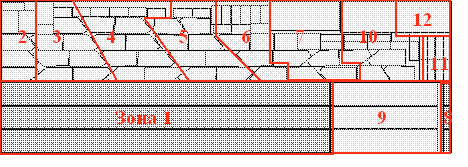
\includegraphics[width=0.9\textwidth]{zones.png}
  \caption{Пример формирования зон резки с учетом <<жесткости>> материала}
  \label{zones}
  \end{center}
\end{figure}

{\bf Заключительные замечания.}
В настоящее время в научных публикациях по теме настоящей монографии
наименее изученными остаются вопросы математической формализации ограничений,
связанных именно с технологическими требованиями термической резки.
Следует отметить, что правила <<жесткости заготовки>> и <<жесткости материала>>
целесообразно учитывать (как показала практика)
не только при разработке управляющих программ для машин газовой,
плазменной и лазерной резки с ЧПУ,
но и при применении машин гидроабразивной фигурной листовой резки.
Этот факт свидетельствует о том,
что изменения геометрических характеристик материала
связано не только с термическими деформациями,
но и с механическими трансформациями материала
при листовой резке заготовок на машинах с ЧПУ.
Рекламные заявления некоторых производителей
лазерных и гидроабразивных машин с ЧПУ о незначительных
деформациях вырезаемых заготовок при листовой фигурной
резке на данных типах технологического оборудования с ЧПУ
опровергаются практическими исследованиями.
Разумеется, лазерная и гидроабразивная технологии
порождают меньшие проблемы с тепловыми деформациями материала,
чем газовая и плазменная,
но не исключают полностью геометрические искажения формы заготовок при резке.

Если обозначить через
$ROUTE_\nu$
частичный маршрут резки первых $\nu$
сегментов
$\nu < K$
\begin{equation}
  ROUTE_\nu = (M_0, M_1, S_1, M_1^*, \dots M_\nu, S_\nu, M_\nu^*, i_1, i_2, \dots i_\nu)
\end{equation}
то правила <<жесткости заготовки>> и <<жесткости материала>>
при формировании допустимого маршрута
$ROUTE$
помимо соблюдения условий предшествования для перестановки
$i_1, i_2, \dots i_K$
и условий (\ref{pierce-constraint}) и (\ref{tool-off-constraint})
формирует следующее дополнительное условие:
если
$ROUTE_\nu$ - частичный маршрут,
допустимый с точки зрения всех технологических
требований листовой резки 1)-3),
сформулированных в этом параграфе,
то сегмент с номером $\nu+1$
и соответствующая точка врезки $M_{\nu+1}$
для него в маршруте
$ROUTE_{\nu+1}$
должны выбираться с учетом уже выбранного частичного маршрута
$ROUTE_\nu$,
что фактически означает либо запрет
на некоторые <<плохие>> номера сегментов
$i_{\nu+1}$
и <<плохие>> точки врезки
$M_{\nu+1}$
в области  $G_M$,
либо наложение <<штрафа>> на <<плохие>> значения
этих параметров кортежа
посредством включения наложенного штрафа в целевые функции
(\ref{cutting-time}) – (\ref{cutting-cost-multi})
при решении оптимизационной задачи (\ref{problem-statement}).

Таким образом,
условия <<жесткости заготовки>> и <<жесткости материала>>
порождают для задачи непрерывно-дискретной оптимизации (\ref{problem-statement})
своего рода динамические ограничения,
формируемые только в процессе вычисления допустимого решения задачи.
В параграфе 2.1
%%% TODO ^^^^^^^^^^^^^^^ fix reference
настоящей монографии будут изложены
некоторые способы математической формализации динамических ограничений,
и описаны алгоритмы оптимизации,
учитывающие эти ограничения.





\section{Классификация оптимизационных задач маршрутизации инструмента машин фигурной листовой резки с ЧПУ}

Существующая  классификация задач маршрутизации инструмента
машин фигурной листовой резки с ЧПУ определяется
типом использованной техники резки и способом задания
возможных точек входа инструмента в контур.
В \cite{intro13}
все задачи маршрутизации разбиты на пять (5) основных классов
(см. Рис. \ref{dewil}).

\begin{itemize}
\item Задача непрерывной резки (CCP, Continuous Cutting Problem):
каждый контур вырезается целиком,
и резка может начаться в любой точке контура (и в ней же завершиться).
Переход к следующему контуру осуществляется на холостом ходу инструмента машины с ЧПУ.

\item Задача коммивояжера  (TSP, Traveling Salesman Problem):
самый простой частный  случай задачи CCP –
каждый контур вырезается целиком,
и резка может начаться в только в одной заранее определенной точке контура
(и в ней же завершиться).

\item Обобщенная задача коммивояжера (GTSP, Generalized Traveling Salesman Problem):
также частный случай задачи CCP –
резка может начаться только в одной из заранее
заданных точек на контуре (их может быть несколько),
контур также должен быть вырезан целиком.

\item Задача резки с конечным набором точек (ECP, Endpoint Cutting Problem):
резка может начаться только в одной из
заранее заданных точек на контуре,
однако контур может быть вырезан за несколько подходов, по частям.

\item Задача произвольной резки (ICP, Intermittent Cutting Problem)
– наиболее общая формулировка задачи моделирования траектории резки,
когда не накладывается никаких ограничений на выбор точек начала и конца резки,
а также на последовательность резки контуров и их частей:
контуры могут резаться по частям,
за несколько подходов и резка может быть
начата и продолжена в любой точке контура.

\end{itemize}

\begin{figure}
  \begin{center}
  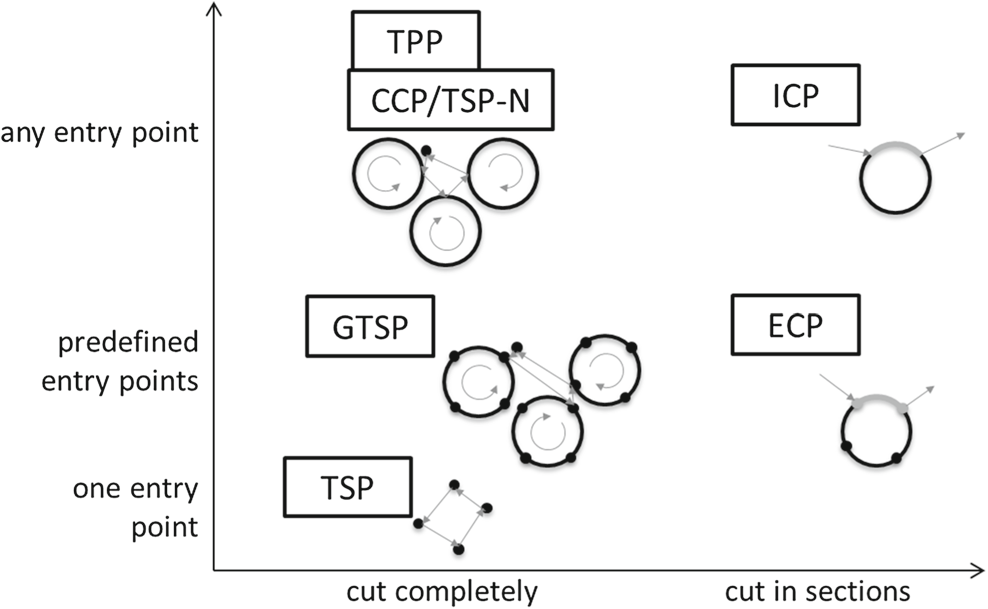
\includegraphics[width=0.9\textwidth]{dewil.png}
  \caption{Основные классы задач маршрутизации инструмента для машин фигурной листовой резки }
  \label{dewil}
  \end{center}
\end{figure}

Обычно предполагается также,
что точки врезки в материал,
которые из-за технологических требований резки
(\ref{pierce-constraint})
не совпадают с точками входа в контур,
однозначно определяются выбранными точками входа в контуры (и наооборот)
и находятся от контуров на фиксированном расстоянии.
Отметим, что число сегментов резки К в кортеже (\ref{tuple})
$ROUTE = (
  M_0, M_1, S_1, M_1^*, M_2, S_2, M_2^*, \dots M_K, S_K, M_K^*, i_1, i_2, \dots i_K
)$
для первых трех классов задач маршрутизации всегда равно количеству вырезаемых контуров $N$.

Введем следующее определение:



{\it Определение 2}:
{\bf Базовым сегментом резки}
$B^S$
для сегмента резки
$S=MM^*$
будем называть часть траектории сегмента
не содержающую траектории входа в контур
lead-in и выхода из контура lead-out, т.е.

\begin{equation}
S=MM^* = M lead_{in} B^S lead_{out} M^*
\label{base-segment}
\end{equation}

Будем полагать,
что базовый сегмент в отличие от сегмента резки
не имеет направления,
но тогда если базовый сегмент содержит
один или более замкнутых контуров,
то при определении сегмента резки $S$
нам необходимо для каждого контура задать направление резки
(<<+>> при резке <<по часовой стрелке>>, <<->> <<против часовой>>).

Таким образом,
каждый базовый сегмент резки
содержит список
$L(B^S)$
своих замкнутых контуров (может быть пустой).
Пусть
$|L(B^S)|$
длина этого списка, тогда кортеж $ROUTE$ (\ref{tuple})
в терминах базового сегмента резки запишется в следующем виде:

\begin{multline}
  ROUTE = (
    M_0, M_1 B^{S_1} M_1^* p_1^1 \dots p_1^{L(B^{S_1})|},
    M_2 B^{S_2} M_2^* p_2^1 \dots p_2^{L(B^{S_2})|},
    \dots, \\
    M_K B^{S_K} M_K^* p_K^1 \dots p_K^{L(B^{S_K})|},
    i_1, i_2, \dots i_K
  )
  \label{tuple-base-segments}
\end{multline}
где $p_t^r=\pm 1$
(направление резки в контуре с номером $r$ базового сегмента  $B^{S_t}$,
$r=\overline{1, |L(B^{S_t})|}$.

Формула (\ref{tuple-base-segments})
дает наиболее общее формальное описание маршрута резки (траектории интрумента)
машины листовой резки с ЧПУ.

В примере резки двух деталей
на рис. \ref{cut2-1}
два базовых сегмента выделены пунктирными
желтой и коричневой линиями
(использована мультиконтурная техника резки).
Пример сегмента резки, в котором использована техника совмещенного реза,
и  базовым сегментом, содержащим четыре контура,
приведен на рис. \ref{cut4-3}.
Черными стрелками отмечено направление резки контуров.

\begin{figure}
  \begin{center}
  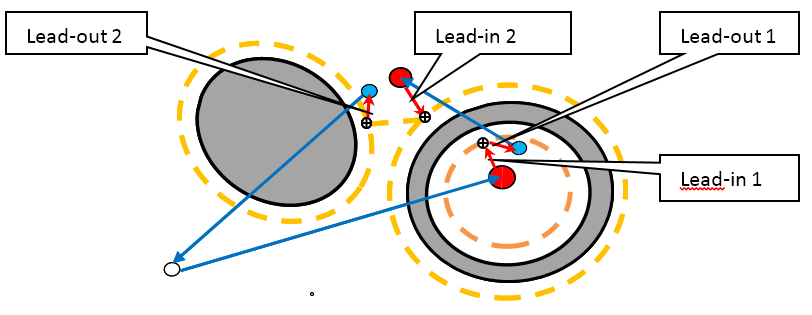
\includegraphics[width=0.9\textwidth]{cut2-1.png}
  \caption{Пример схемы резки трех замкнутых контуров с использованием двух сегментов резки}
  \label{cut2-1}
  \end{center}
\end{figure}

\begin{figure}
  \begin{center}
  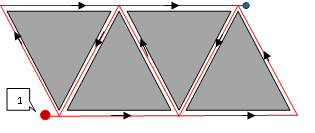
\includegraphics[width=0.7\textwidth]{cut4-3.png}
  \caption{Сегмент резки, включающий базовый сегмент с использованием техники резки <<совмещенный рез>>}
  \label{cut4-3}
  \end{center}
\end{figure}

На основе концепции базового сегмента введем еще
два класса задач маршрутизации инструмента машин
фигурной листовой резки с ЧПУ

{\it Определение 3}:
SCCP (Segment Continuous Cutting Problem)
задача с фиксированным числом $K$
сементов резки (и базовых сегментов резки
$B^{S_k}, k = \overline{1, K}$).

{\it Замечание}:
Если все граничные контуры деталей
$C_1, C_2 \dots C_N$
базовые сегменты $B^{S_k}, k = \overline{1,K}$,
и $N=K$
тогда SCCP эквивалентна CCP.

Предположим, что для исходной задачи маршрутизации
определен конечный набор (ансамбль)
базовых сегментов резки размерности $T$.
Этот ансамбль соответствует ансамблю задач
$\{SCCP_i, i =\overline{1,T}\}$.

{\it Определение 4}:
GSCCP (Generalized SCCP) -- есть
$\{SCCP_i, i =\overline{1,T}\}$

Как нетрудно видеть,
введя классы SCCP и  GSCCP,
мы значительно расширили существующую
классификацию задач маршрутизации инструмента
для машин листовой резки с ЧПУ.
Фактически SCCP и GSCCP являются подклассами ICP,
содержащими все задачи с конечным набором базовых сегментов резки,
т.е.
$CCP \subset SCCP \subset GSCCP \subset ICP$
Таким образом, в классе ICP выбран большой подкласс
задач маршрутизации,
для которых можно разработать эффективные алгоритмы оптимизации.

На рис. \ref{x-classify}
приведена расширенная классификация этих задач.
Как видно из данного  рисунка,
все классы сгруппированы в три группы
различающиеся мощностью множеств,
из которых выбираются точки входа в контуры
(точки врезки).

\begin{figure}
  \begin{center}
  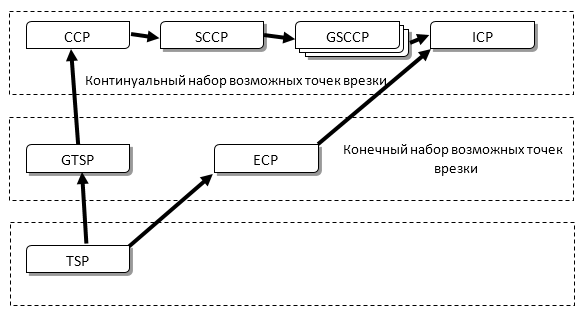
\includegraphics[width=0.9\textwidth]{x-classify.png}
  \caption{Расширенная классификация задач маршрутизации инструмента машин листовой резки }
  \label{x-classify}
  \end{center}
\end{figure}

Рассмотрим далее подход,
основанный на  дискретизации трех клаcсов задач маршрутизации
первой группы (CCP, SCCP, GSCCP)
и сведении их к задаче о последовательном обходе мегаполисов,
в которой  используется математическая модель А.Г.Ченцова,
описанная подробно во второй части настоящей монографии
(главы 3-5).

Эта модель может быть интерпретирована
как математическая модель обобщенной задачи коммивояжера (GTSP)
с дополнительными ограничениями.
(Следует различать модель GTSP и задачу маршрутизации GTSP из второй группы,
которая представляеи собой дискретный вариант задачи CCP).
В отличие от классического GTSP эта модель
предусматривает учет так называемой внутренней работы
(в данном случае, процесса резки).
Кроме того, модель мегаполисов с
использованием специальной схемы динамического программирования
учитывает сложные типы целевых функций и сложные ограничения,
в том числе динамические.
Наконец, принимая во внимание ограничения предшествования,
можно получить точные решения для дискретных вариантов SCCP
достаточно большой размерности.

В качестве примера рассмотрим задачу GSCCP,
которая содержит две (2)
задачи SCCP с разными наборами сегментов,
показанными на рисунке \ref{gsccp-both}
(21 базовый сегмент – \ref{gsccp-a}
и 18 – \ref{gsccp-b} соответственно).

\begin{figure}
  \centering
  \subfigure[21 базовый сегмент]{
    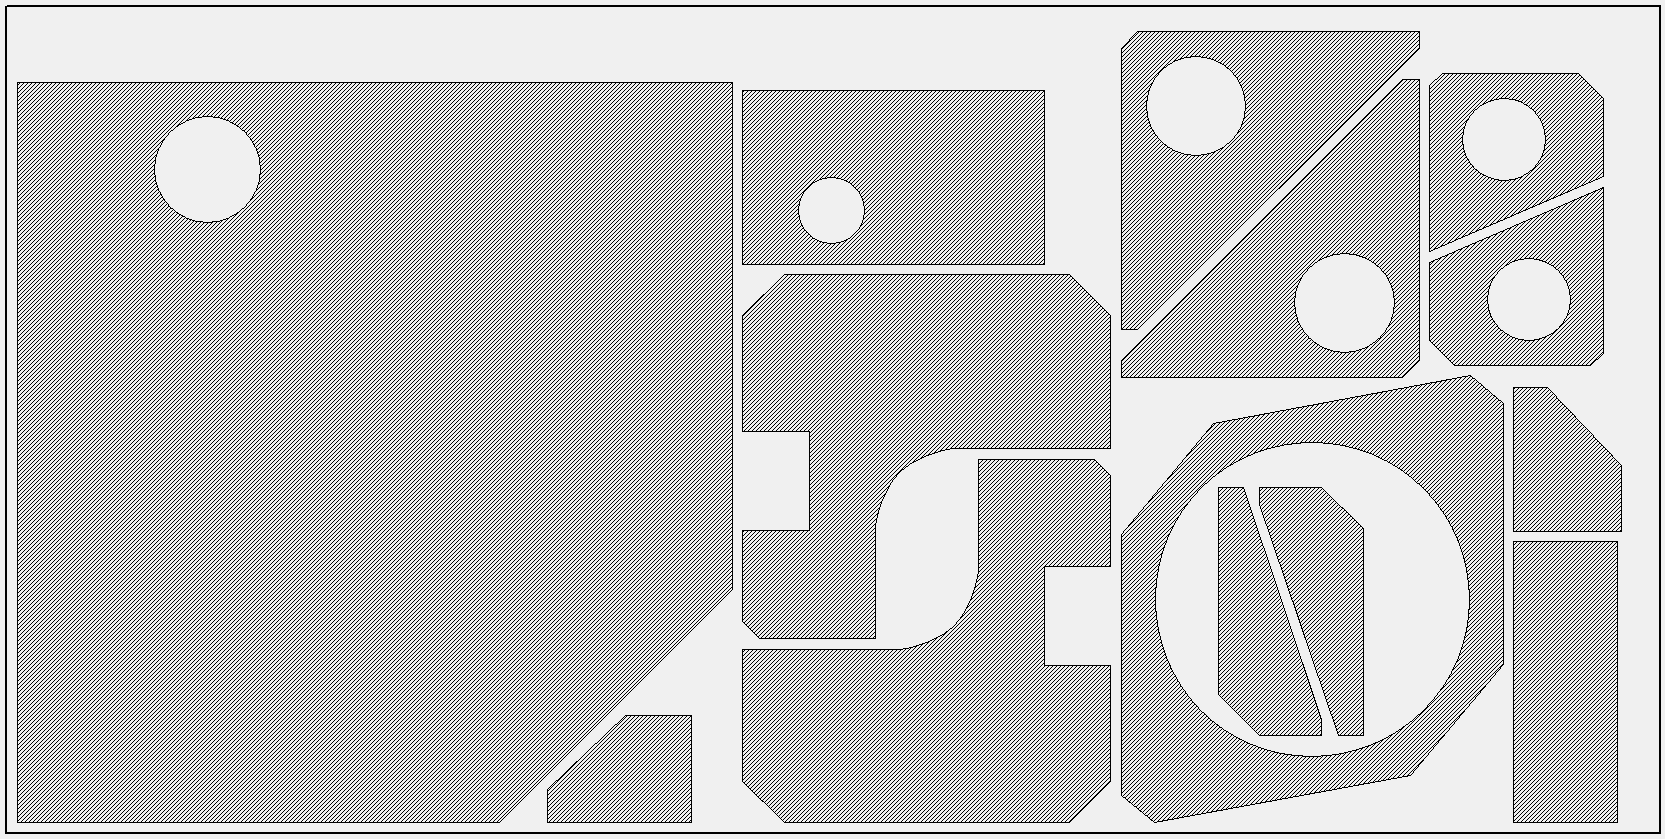
\includegraphics[width=0.4\textwidth]{gsccp-a.png}
    \label{gsccp-a}
  }
  \subfigure[18 базовых сегментов]{
    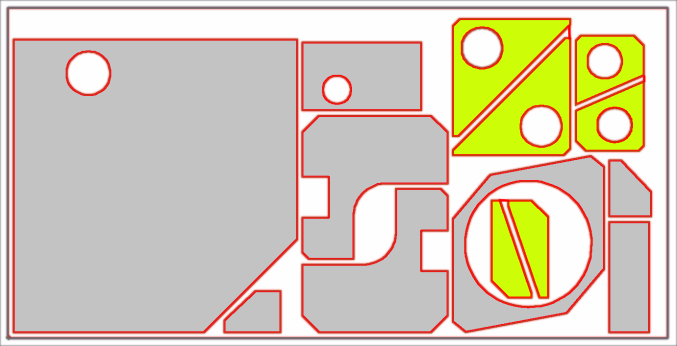
\includegraphics[width=0.4\textwidth]{gsccp-b.png}
    \label{gsccp-b}
  }
  \caption{Пример задачи GSCCP с набором из двух комплектов базовых сегментов}
  \label{gsccp-both}
\end{figure}

Первый набор базовых сегментов (Рис. \ref{gsccp-a})
задан всеми граничными контурами деталей, т.е.
$C_j = B^{S_j}, j=\overline{1,N}, N=K=21$.
В этом случае мы имеем классическую задачу CCP.
На рис. \ref{gsccp-b} восемь (8)
базовых сегментов заданы внешними граничными контурами <<серых>> деталей.
Три (3) дополнительных базовых сегмента заданы шестью (6)
внешними граничными контурами <<цветных>> деталей
(один базовый сегмент состоит из двух внешних контуров плюс перемычка между ними).
Эти контуры будут вырезаться <<цепной>> резкой попарно в одном базовом сегменте.
Наконец семь (7) базовых сегментов заданы внутренними
граничными контурами всех деталей,
в которых имеются отверстия.
В целом, в этом случае мы имеем набор из восемнадцати (18)
базовых сегментов.
Все они выделены красным цветом.
В качестве целевой функции для данного примера была выбрана функция - время процесса резки (\ref{cutting-time}):
$$
T_{cut} = \frac{L_{on}}{V_{on}} + \frac{L_{off}}{V_{off}} +N_{pt} \cdot t_{pt}
$$

Чтобы свести непрерывные задачи SCCP
к дискретной модели,
каждый базовый сегмент делится с определенным шагом по точкам,
которые будут претендентами на точку входа инструмента в контур.
Каждая такая точка входа однозначно определяет точку врезки.
В то же время каждая возможная точка врезки должна
удовлетворять технологическим ограничениям процесса резки
(\ref{pierce-constraint}),
то есть многие точки базовых сегментов будут удалены.
Напомню, что для каждого базового сегмента
такая точка может быть только одна.
На рис. \ref{discrete21}
показан конечное множество возможных точек врезки
(выделены зеленым цветом)
для первой задачи
(набор из двадцати одного базового сегмента).
Фактически мы свели первую задачу SCCP
(в данном конкретном случае эквивалентную CCP)
(Рис. \ref{gsccp-a})
к задаче о последовательном обходе мегаполисов (модели GTSP).
Обратите внимание,
что в этом случае число возможных маршрутов резки $ROUTE$
становится конечным.
Процесс дискретизации второй задачи SCCP \ref{gsccp-b}
производится аналогичным образом.
Для решения обеих задач применен метод динамического программирования,
использующий специальную схему Беллмана,
которая будет описана во второй части монографии.

\begin{figure}
  \begin{center}
  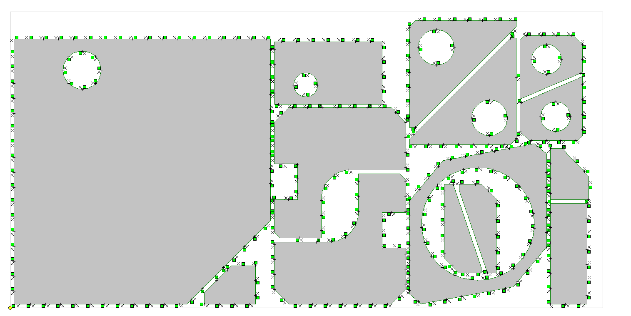
\includegraphics[width=0.9\textwidth]{discrete21.png}
  \caption{Дискретизация задачи CCP, приведенная на рисунке \ref{gsccp-a}}
  \label{discrete21}
  \end{center}
\end{figure}

На рисунках \ref{path21}
и \ref{path18}
показаны оптимальные маршруты резки для двух задач SCCP
с двацать одним (21) и восемнадцатью (18)
базовыми сегментами соответственно.

\begin{figure}
  \begin{center}
  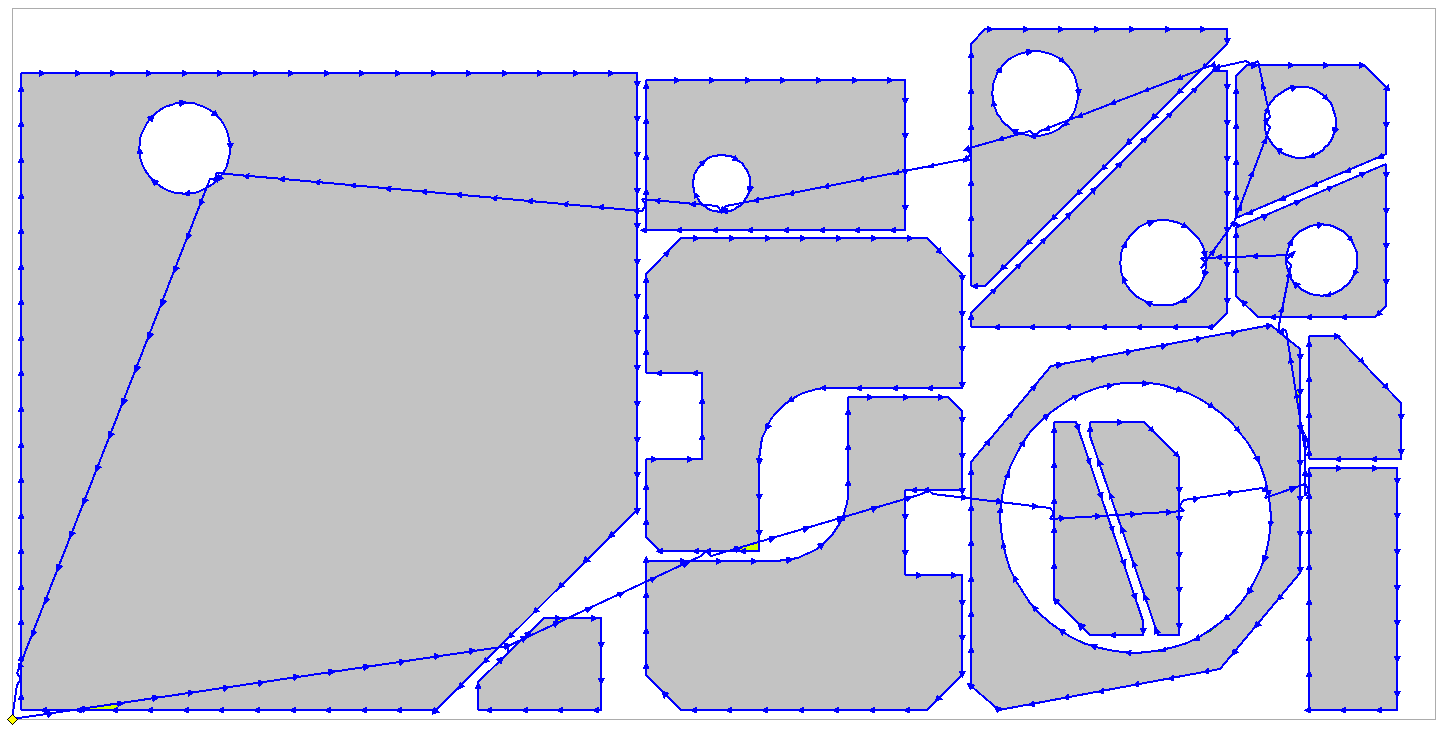
\includegraphics[width=0.9\textwidth]{path21.png}
  \caption{Схема оптимальной траектория инструмента для 21 базового сегмента}
  \label{path21}
  \end{center}
\end{figure}

\begin{figure}
  \begin{center}
  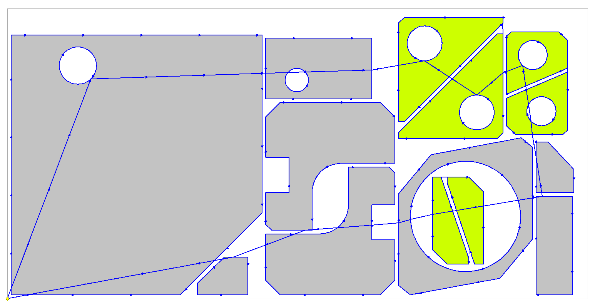
\includegraphics[width=0.9\textwidth]{path18.png}
  \caption{Схема оптимальной траектория инструмента для 18 базового сегмента}
  \label{path18}
  \end{center}
\end{figure}

В первом случае время процесса резки
$T_{cut}$
составляет 2255 секунд,
во втором - 2244 секунды.
Обратите внимание, что в первом случае длина рабочего хода инструмента
$L_{on}$
(20567 мм) меньше, чем во втором – (20727 мм),
но из-за уменьшения количества точек прокалывания
для 18 сегментов общее время резки также уменьшилось.
Еще раз отметим, что оба решения являются оптимальными
для выбранных наборов базовых сегментов.
Таким образом, оптимальное значение целевой
функции для выбранной задачи GSCCP составляет 2244 сек.

При решении задач были учтены необходимые <<статические>> ограничения:
условия предшествования и ограничения для координат
точек врезки (\ref{pierce-constraint}).
Динамические ограничения в этом модельном примере не рассматривались.

Описанный подход позволяет решать задачи из
наиболее сложного класса задач маршрутизации
траектории инструмента - ICP,
который не ограничивает выбор точки входа
инструмента в контур детали и использование
любой техники резки.
Наиболее важной особенностью подхода
является возможность для одной задачи оптимизации
формировать разные наборы базовых сегментов и
применять разные алгоритмы оптимизации,
используя как дискретные, так и,
в некоторых случаях, непрерывные модели.
















\chapter{ПРАКТИЧЕСКИЕ АСПЕКТЫ ОПТИМИЗАЦИИ ТРАЕКТОРИИ ИНСТРУМЕНТА ДЛЯ МАШИН ЛАЗЕРНОЙ РЕЗКИ С ЧПУ}
%\setcounter{section}{1}\setcounter{subsection}{1}
\setcounter{chapter}{2}
\setcounter{equation}{0}

\section{Точное вычисление целевых функций в задаче оптимизации маршрута резки на примере машины лазерной резки ByStar3015}

Как мы уже  отмечали в \S 1.2
%%% TODO fix reference  ^^^^^^^^^^^^^^^
для задачи оптимизации маршрута резки (\ref{problem-statement})
проблема точного вычисления целевых функций времени резки и стоимости резки,
определяемых, в частности, формулами (\ref{cutting-time}) и (\ref{cutting-cost}):
$$
T_{cut} = \frac{L_{on}}{V_{on}} + \frac{L_{off}}{V_{off}} +N_{pt} \cdot t_{pt}
$$
$$
F_{cost}=
L_{on} \cdot C_{on} +
L_{off} \cdot C_{off} +
N_{pt} \cdot C_{pt}
$$
является малоисследованной.
Ниже будут приведены результаты исследований,
проведенных А.Ф.Таваевой на предприятии
АО <<Производственное объединение <<Уральский оптико – механический завод>>
имени Э.С. Яламова>> (Екатеринбург)
на машине лазерной резки ByStar3015.
Более подробно результаты этих исследований изложены в
\cite{intro45,intro46,intro47}.

\subsection{Вычисление фактического времени лазерной резки машины с ЧПУ
в зависимости от параметров управляющей программы и технологических факторов процесса резки}

Неточность вычисления фактического времени резки
$T_{cut}$
связана с тем, что скорость рабочего хода машины с ЧПУ
$V_{on}$,
программируемая в управляющей программе как константа,
фактически таковой не является и может меняться
в зависимости от различных технологических факторов,
а также характеристик спроектированной управляющей программы.
В частности, было установлено,
что при увеличении числа кадров в управляющих программах
резки разных наборов заготовок,
имеющих один и тот же суммарный периметр контуров,
фактическая средняя скорость резки падает.
Причины, по которым УП могут содержать большое количество кадров,
в основном, связано с тем, что контуры со сложной геометрией
(например, сплайны) при конвертации из CAD системы в CAM
модуль из-за разницы в геометрических форматах файлов
разбиваются на большое число геометрических примитивов
(например, на отрезки прямых и дуги окружностей),
т.е. аппроксимируются более простыми геометрическими примитивами.
Разница в форматах, в свою очередь,
вызвана тем, что практически все системы ЧПУ
оснащаются только линейными и круговыми интерполяторами.
Как правило, аппроксимация сложной геометрии сводится
именно к линейной аппроксимации.
Иногда конвертеры CAD файлов аппроксимируют отрезками прямых
даже дуги окружностей, хотя в этом нет необходимости,
если система ЧПУ поддерживает круговую интерполяцию.

Ниже приведены некоторые практические результаты
по определению зависимости скорости рабочего хода
инструмента лазерного комплекса ByStar3015
от количества кадров управляющей программы.

Исследования были проведены для следующих материалов:
10кп ($\Delta$=1-10мм) и АМг3М ($\Delta$=1-5мм).
Для проведения вычислительных экспериментов были разработаны
150 тестовых УП для резки различных фигурных заготовок с числом кадров
$n \in \overline{10,5000}$
для материала 10кп и 150 УП – для материала АМг3М с числом кадров
$n \in \overline{10,2000}$.

Статистический материал был обработан в программе <<Mathcad>>
и с помощью метода наименьших квадратов были построены
аппроксимирующие функции для зависимости скорости
рабочего хода инструмента
$V_{on}$
от количества кадров в спроектированной УП.
По результатам эксперимента были сделаны следующие выводы:

\begin{enumerate}
\item Фактическая средняя скорость рабочего хода режущего инструмента
$V_{on}$
является монотонно убывающей функцией от числа кадров УП
(рис. \ref{amg3m}, \ref{10kp});

\item Заданная в УП скорость
$V_{on}$
совпадает с фактической средней скоростью
при достижении числом кадров некоторого порогового значения $N$.
Когда количество кадров в УП меньше порогового значения $n<N$,
то фактическая скорость выше заданной,
а при увеличении числа кадров больше порогового $n>N$
– может существенно снижаться
(в проведенных экспериментах снижение средней
фактической скорости режущего инструмента по сравнению
с заданным в УП значением доходило до 70\%);

\item Пороговое значение различно для разных марок материала и толщин.

\end{enumerate}

Для изложения результатов вычислительных экспериментов
введем следующие обозначения:
пусть
$n$  – число кадров в УП,
$V_\text{факт}$  – фактическая средняя скорость режущего инструмента при заданной скорости $V_{on}$,
$N$ - число кадров (пороговое значение), для которого $V_\text{факт}=V_{on}$;
$\sum \varepsilon_n^2$  - сумма квадратов отклонений исходных значений
скорости режущего инструмента и значений аппроксимирующей функции $V_{on}(n)$
в этих точках.

При аппроксимации точечных графиков
зависимости фактической скорости
$V_\text{факт}$
от числа кадров $n$
в УП аппроксимирующими кривыми в <<Mathcad>>
для всех значений исследуемых марок материала и толщин материала было установлено,
что сходимость
$\sum \varepsilon_n^2 \to 0$
достигается при аппроксимации экспериментальных данных логарифмической функцией.

Аналогичные результаты были получены для материала АМг3М $\Delta$=2-5мм и 10кп $\Delta$=1-10мм.
Обобщенные результаты для всех исследованных марок материала и толщин приведены в табл. \ref{v-formulae}.

При использовании материала других марок
необходимо проведение дополнительных исследований,
либо использование имеющихся данных по материалу
с близкими физическими свойствами.

\begin{figure}
  \begin{center}
  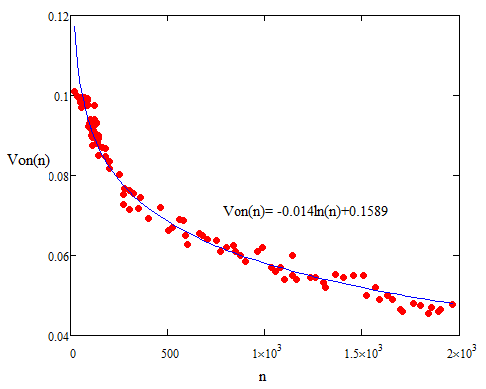
\includegraphics[width=0.7\textwidth]{amg3m.png}
  \caption{Изменение скорости режущего инструмента на рабочем ходу для АМг3М, $\Delta$=1мм
($n \in \overline{10,2000}$)}
  \label{amg3m}
  \end{center}
\end{figure}


\begin{figure}
  \begin{center}
  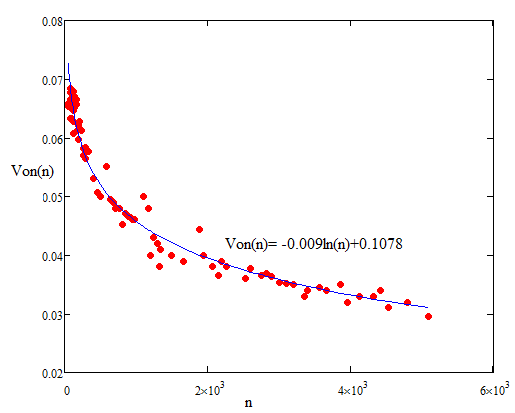
\includegraphics[width=0.7\textwidth]{10kp.png}
  \caption{Изменение скорости режущего инструмента на рабочем ходу для 10кп, $\Delta$=3мм
($n \in \overline{10,5000}$)}
  \label{10kp}
  \end{center}
\end{figure}

\begin{table}
  \caption{Обобщенная таблица формул для вычисления рабочей скорости инструмента
  на лазерном комплексе ByStar3015}
  \label{v-formulae}
  \centering
  \begin{tabular}{lll}
    \hline
    Материал & Толщина, мм & Формула расчета $V_{on}$ \\
    \hline
    \multicolumn{3}{c}{$n=\overline{10,5000}$} \\
    10кп & 1 & $V_{on} = -0.024 \ln n+0.245$ \\
    10кп & 2 & $V_{on} = -0.015 \ln n+0.1686$ \\
    10кп & 3 & $V_{on} = -0.009 \ln n+0.1078$ \\
    10кп & 3.5 & $V_{on} = -0.006 \ln n+0.0756$ \\
    10кп & 4 & $V_{on} = -0.006 \ln n+0.0709$ \\
    10кп & 8 & $V_{on} = -0.003 \ln n+0.0442$ \\
    10кп & 10 & $V_{on} = -0.002 \ln n+0.0365$ \\
    \multicolumn{3}{c}{$n=\overline{10,2000}$} \\
    АМг3М & 1 & $V_{on} = -0.014 \ln n+0.1589$ \\
    АМг3М & 1.5 & $V_{on} = -0.001 \ln n+0.011$ \\
    АМг3М & 3 & $V_{on} = -0.004 \ln n+0.0672$ \\
    АМг3М & 4 & $V_{on} = -0.001 \ln n+0.0301$ \\
    АМг3М & 5 & $V_{on} = -6\cdot 10^{-4} \ln n+0.0177$ \\
  \end{tabular}
\end{table}

Рассмотрим пример оптимизации времени резки
$T_{cut}$
(\ref{cutting-time})
при резке 15 фигурных заготовок
(материал АМг3М, $\Delta$=1мм).
Раскройная карта (рис. \ref{amg-cutting})
содержит 15 заготовки двух типоразмеров,
при этом количество граничных контуров заготовок равно 19.
Каждый контур вырезается с помощью резки
<<по замкнутому контуру>>.
С целью сокращения множества допустимых решений
задачи множество возможных точек врезки было
ограничено конечным множеством (задача GTSP),
состоящим из 55 точек
(обозначены маленькими квадратиками;
соответствующие точки выключения инструмента обозначены крестиками).
Для решения задачи использован точный алгоритм на основе ДП.
УП резки для данного примера содержат 120 команд или кадров
(т.е. $n=120$),
которые включают команды перемещения инструмента
для резки контуров
(с учетом разбиения каждого контура на несколько геометрических примитивов)
на рабочем ходу,
команды перемещения инструмента на холостом ходу
и ряд технологических команд.
Скорость рабочего хода инструмента, заданная в УП,
$V_{on}=0.1$ м/с.

\begin{figure}
  \begin{center}
  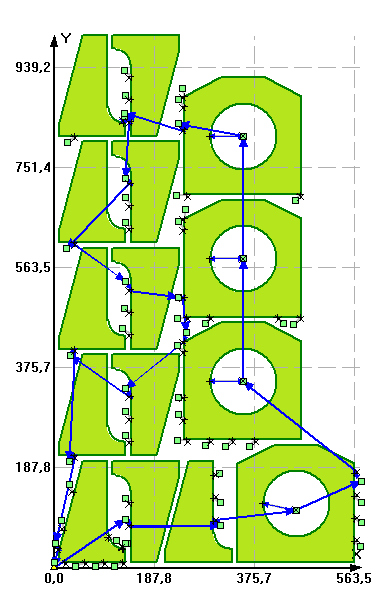
\includegraphics[width=0.5\textwidth]{amg-cutting.png}
  \caption{Раскройная карта и оптимальный по времени маршрут
  перемещения режущего инструмента для 15 заготовок (материал АМг3М, $\Delta$=1мм) при условии, что
  $V_{on}=const=0.1$м/с}
  \label{amg-cutting}
  \end{center}
\end{figure}

На рис. \ref{amg-cutting}
показан маршрут резки
(перемещение инструмента на холостом ходу показаны стрелками),
для которого значение целевой функции
$T_{cut}$ (\ref{cutting-time})
при
$V_{on}=0.1$ м/с
составляет
$T_{cut}=126.27$ сек.
Однако фактическое время резки по управляющей программе,
составленной для этого маршрута, оказалось (как и ожидалось)
значительно больше,
поскольку число кадров в программе ($n=120$)
значительно больше порогового значения $N=70$
для материала АМг3М $\Delta$=1мм.

При использовании значения
$V_{on}=-0.014 \ln n + 0.1589$
(табл.6) в целевой функции (\ref{cutting-time})
оптимизационная процедура ДП
дает другое оптимальное решение задачи,
которое показано на рис. \ref{amg-optimal}.
Тогда среднее фактическое значение рабочей скорости инструмента при $n=120$
составило
$V_{on}=0.0919$ м/с.
В свою очередь для оптимального маршрута резки значение времени резки составило
$T_{cut}=141.38$ сек.

Таким образом,
точное вычисление целевой функции для
данного примера обеспечило не только
точное вычисления значения экстремума
целевой функции, но и другой (правильный)
результат поиска оптимального маршрута резки,
полученный  с учетом числа кадров УП.


\begin{figure}
  \begin{center}
  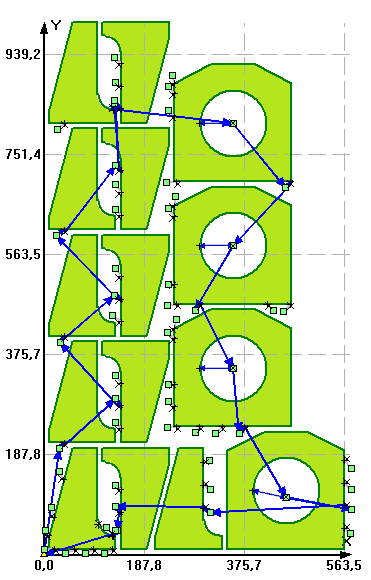
\includegraphics[width=0.5\textwidth]{amg-optimal.png}
  \caption{Оптимальный по времени маршрут перемещения режущего инструмента при условии, что
  $V_{on}=-0.014 \ln n + 0.1589$
  $(n=120)$}
  \label{amg-optimal}
  \end{center}
\end{figure}

Данный пример иллюстрирует необходимость
получения таблиц типа Таблицы \ref{v-formulae}
при решении конкретных оптимизационных задач
маршрутизации инструмента машин листовой резки с ЧПУ.

\subsection{Вычисление стоимости резки заготовок на машине с ЧПУ в режиме моделирования процесса резки}

Другая проблема точного вычисления целевой функции
при оптимизации маршрута резки связано
с поиском адекватных значений стоимости в формуле (\ref{cutting-cost}):
$$
F_{cost}=
L_{on} \cdot C_{on} +
L_{off} \cdot C_{off} +
N_{pt} \cdot C_{pt}
$$

Напомним:
$C_{on}$ – стоимость единицы пути с включенным режущим инструментом;
$C_{off}$ – стоимость единицы пути с выключенным режущим инструментом;
$C_{pt}$ – стоимость одной точки врезки,
$L_{off}$ – длина переходов с выключенным режущим инструментом (холостой ход);
$L_{on}$ – длина реза с включенным режущим инструментом;
$N_{pt}$ – количество точек врезки.

Рассмотрим вопрос точного вычисления
стоимости лазерной резки в задаче
оптимизации маршрута режущего инструмента
применительно к машине лазерной резки (тип лазера: СО$_2$)
с ЧПУ на примере машины ByStar3015.

Проблема точного вычисления целевой функции
при оптимизации маршрута резки связана с
поиском адекватных значений стоимости
$F_{cost}$,
вычисление которой зависит от параметров
$C_{on}, C_{off}, C_{pt}$.

Для расчета
$C_{on}$
введем следующие обозначения для стоимостных параметров,
вычисляемых на 1 м рабочего хода инструмента:
$C_\text{расх}$   - стоимость расходных материалов (например, сопло, защитное стекло, газовые трубки);
$C_\text{тех}$   - стоимость технологического газа (азот или кислород в зависимости от типа обрабатываемого материала);
$C_\text{лаз}$ - стоимость лазерного газа (при работе на машине с ЧПУ на проточном газовом лазере),
$C_\text{э/э}^{on}$ - стоимость электроэнергии;
$C_\text{зп}^{on}$ - затраты, связанные с заработной платой сопровождающего персонала;
$C_\text{А}^{on}$ - амортизация оборудования.
Тогда в общем виде
$C_{on}$
будем вычислять по следующей формуле:

\begin{equation}
  C_{on} =
  C_\text{э/э}^{on} +
  C_\text{тех} +
  C_\text{лаз} +
  C_\text{расх} +
  C_\text{зп}^{on} +
  C_\text{А}^{on}
  \label{c-on}
\end{equation}

Для вычисления значений
$C_{on}, C_\text{э/э}^{on}, C_\text{тех}, C_\text{лаз}, C_\text{расх}, C_\text{зп}^{on}, C_\text{А}^{on}$
введем дополнительные обозначения:
$t_{on}$ – время, затрачиваемое на один метр рабочего хода инструмента, час;
$P_{on}$ – затраты электроэнергии за один час работы лазерного комплекса на рабочем ходу, кВт/ч;
$V_\text{тех}$ – расход технологического газа, м$^3$/ч;
$V_\text{лаз}$ – расход лазерного газа, м$^3$/ч;
$C_\text{э/э}$ - стоимость электроэнергии за 1 кВт;
$C_{\text{лазМ}^3}$- стоимость 1м$^3$ лазерного газа;
$C_{\text{техМ}^3}$ - стоимость 1м$^3$ технологического газа;
$C_\text{расхЕд}$- стоимость единицы расходных материалов;
$t_\text{расхСрок}$- срок службы расходных материалов;
$C_\text{зп}$ - стоимость 1ч работы обслуживающего персонала;
$A$ – амортизация за 1 час работы лазерного комплекса, руб;
$N$ – срок полезного использования оборудования, год;
$C_\text{оборуд}$- первоначальная стоимость лазерного комплекса. Тогда
$C_{on}, C_\text{э/э}^{on}, C_\text{тех}, C_\text{лаз}, C_\text{расх}, C_\text{зп}^{on}, C_\text{А}^{on}$
вычислим по следующим формулам:

\begin{equation}
  C_\text{э/э}^{on} =
  P_{on} t_{on}   C_\text{э/э}
  \label{c-on-ee}
\end{equation}

\begin{equation}
  C_\text{тех} =
  V_\text{тех} C_{\text{техМ}^3} t_{on}
  \label{c-on-teh}
\end{equation}

\begin{equation}
  C_\text{лаз} =
  V_\text{лаз} C_{\text{лазМ}^3} t_{on}
  \label{c-on-laz}
\end{equation}

\begin{equation}
  C_\text{расх} =
  \frac{C_\text{расхЕд}}{t_\text{расхСрок}}
  \label{c-on-rasx}
\end{equation}

\begin{equation}
  C_\text{зп}^{on} =
  C_\text{зп} t_{on}
  \label{c-on-zp}
\end{equation}

\begin{equation}
  C_\text{А}^{on} =
  \frac{1}N \frac{C_\text{оборуд}}{1920} t_{on}
  \label{c-on-A}
\end{equation}

Параметр
$C_\text{тех}$
необходимо учитывать при расчете стоимости резки
только в тех случаях,
когда применяется вспомогательный рабочий газ
(кислород, азот в зависимости от типа обрабатываемого материала)
для увеличения скорости резки,
возможности обработки материалов более высоких толщин
и для сокращения затрат электроэнергии.
Расход газа зависит от диаметра используемого сопла и давления газа.

Для расчета
$C_{off}$
введем следующие обозначения параметров,
вычисляемых на 1 м холостого хода режущего инструмента:
$P_{off}$ – затраты электроэнергии за один час работы лазерного комплекса на холостом ходу, кВт/ч;
$t_{off}$ – время, затрачиваемое на один метр холостого хода инструмента, час.
Тогда

\begin{equation}
  C_{off} =
  P_{off} t_{off} C_\text{э/э}
  + C_\text{зп} t_{off}
  + \frac{1}N \frac{C_\text{оборуд}}{1920} t_{off}
  \label{c-off}
\end{equation}

Аналогично для расчета
$C_{pt}$
введем следующие обозначения для стоимостных параметров,
вычисляемых на одну точку врезки:
$C_\text{э/э}^{pt}$ - стоимость электроэнергии;
$C_\text{расх}^{pt}$ - стоимость расходных материалов;
$C_\text{лаз}^{pt}$– стоимость лазерного газа;
$C_\text{тех}^{pt}$- стоимость технологического газа,
$C_\text{зп}^{pt}$- затраты, связанные с заработной платой сопровождающего персонала;
$C_\text{А}^{pt}$- амортизация оборудования.
Тогда

\begin{equation}
  C_{pt} =
  C_\text{э/э}^{pt} +
  C_\text{расх}^{pt} +
  C_\text{лаз}^{pt} +
  C_\text{тех}^{pt} +
  C_\text{зп}^{pt} +
  C_\text{А}^{pt}
  \label{c-pt}
\end{equation}

Для вычисления значений  ,  ,
$C_\text{э/э}^{pt}, C_\text{расх}^{pt}, C_\text{лаз}^{pt}, C_\text{тех}^{pt}$
введем дополнительные параметры:
$P_{pt}$ - затраты электроэнергии на одну точку врезки, кВт/ч;
$t_{pt}$ – время, затрачиваемое на одну точку врезки, час. Тогда

\begin{equation}
  C_\text{э/э}^{pt} =
  P_{pt} t_{pt}   C_\text{э/э}
  \label{c-pt-ee}
\end{equation}

\begin{equation}
  C_\text{тех}^{pt} =
  V_\text{тех} C_{\text{техМ}^3} t_{pt}
  \label{c-pt-teh}
\end{equation}

\begin{equation}
  C_\text{лаз}^{pt} =
  V_\text{лаз} C_{\text{лазМ}^3} t_{pt}
  \label{c-pt-laz}
\end{equation}

\begin{equation}
  C_\text{расх}^{pt} =
  \frac{C_\text{расхЕд}}{t_\text{расхСрок}}
  \label{c-pt-rasx}
\end{equation}

\begin{equation}
  C_\text{зп}^{pt} =
  C_\text{зп} t_{pt}
  \label{c-pt-zp}
\end{equation}

\begin{equation}
  C_\text{А}^{pt} =
  \frac{1}N \frac{C_\text{оборуд}}{1920} t_{pt}
  \label{c-pt-A}
\end{equation}

При расчете стоимости одной точки врезки параметр
$C_\text{лаз}^{pt}$
необходимо учитывать только при обработке материала
на проточном газовом лазере.
Параметр
$C_\text{тех}^{pt}$
необходимо учитывать при расчете себестоимости резки только в тех случаях,
когда применяется вспомогательный рабочий газ.

Тогда целевую функцию стоимости резки (\ref{cutting-cost})
можно записать в следующем виде:
\begin{multline}
  F_{cost} =
  L_{on} \Big(
    C_\text{э/э}^{on} +
    C_\text{тех} +
    C_\text{лаз} +
    C_\text{расх} +
    C_\text{зп}^{on} +
    C_\text{А}^{on}
      \Big)
  +L_{off} C_{off} +
  \\
+ N_{pt} \Big(
    C_\text{э/э}^{pt} +
    C_\text{расх}^{pt} +
    C_\text{лаз}^{pt} +
    C_\text{тех}^{pt} +
    C_\text{зп}^{pt} +
    C_\text{А}^{pt}
      \Big)
  \label{c-full}
\end{multline}

К основным расходным материалам и запчастям
для газового лазера можно отнести:
поворотные зеркала, фокусирующие линзы,
защитные стекла, сопла, юстировочные узлы,
газовые трубки.
К основным расходным материалам для
волоконного лазера можно отнести:
сопла, защитные стекла, фокусирующие линзы.
А для случая применения твердотельных лазеров
выделяют следующие основные расходные материалы и запчасти:
лампы оптической накачки, защитные стекла, зеркала,
квантрон, активный элемент.
Следует отметить, что стоимость расходных материалов
может изменяться в зависимости от фактических сроков
службы расходных материалов,
которые зависят от качества используемого газа,
опыта персонала, эксплуатирующего лазерный станок.
Следует отметить, что
$C_\text{расхЕд}$
зависит от ценообразования, курса доллара (USD) и евро (EUR),
а параметры
$C_\text{э/э}$,
$C_{\text{лазМ}^3}$ и
$C_{\text{техМ}^3}$
зависят от цен, которые устанавливает поставщик услуг,
поэтому при расчете
$F_{cost}$
для конкретных производственных задач,
изменения цен целесообразно учитывать,
используя изменяющиеся в зависимости от перечисленных
факторов таблицы стоимостных параметров в MS Excel.
В частности, была создана сводная таблица в MS Excel
для расчета себестоимости лазерной резки по разработанной
выше методике для газового СО$_2$
лазерного комплекса ByStar 3015 для следующих материалов:

\begin{itemize}
\item нержавеющая сталь (на примере 12Х18Н10Т) толщиной $\Delta$=1-10мм;

\item углеродистая сталь (на примере 10кп) толщиной $\Delta$=1-15мм;

\item алюминий и его сплавы (на примере АМг3М) толщиной $\Delta$=1-5мм.
\end{itemize}

Были определены значения основных стоимостных характеристик
$C_{on}$, $C_{off}$, $C_{pt}$
с учетом всех перечисленных параметров, приведенных в
(\ref{c-on})-(\ref{c-pt-A}).
В табл. \ref{c-table} приведены значения стоимости
одного погонного метра лазерного реза при максимальной
$C_{on}^{max}$
и минимальной
$C_{on}^{min}$
возможной рабочей скорости перемещения режущего инструмента
$V_{on}$
в зависимости от требуемого качества изготовления деталей.

\begin{table}
  \caption{Значения основных стоимостных параметров при вычислении целевой функции для CO$_2$ лазерного комплекса ByStar3015}
  \label{c-table}
  \centering
  \begin{tabular}{c*{5}{r}}
    \hline
    Материал & Толщина, мм & $C_{on}^{max}$, руб & $C_{on}^{min}$, руб & $C_{off}$, руб & $C_{pt}$, руб \\
    \hline
    10кп	& 1	& 5,3	& 7,5	& 0,42	& 0,7 \\
    10кп	& 1,2	& 6,6	& 9,5	& 0,42	& 1,0 \\
    10кп	& 1,5	&  6,6	& 9,5	& 0,42	& 1,1 \\
    10кп	& 2	& 8,1	& 11,7	& 0,42	& 1,3 \\
    10кп	& 2,5	&	9,7	& 14,0	& 0,42	& 1,5 \\
    10кп	& 3	& 12,0	& 17,4	& 0,42	& 1,6 \\
    10кп	& 3.5	&	13,3	& 19,0	& 0,42	& 1,6 \\
    10кп	& 3.9	&	13,3	& 19,0	& 0,42	& 1,9 \\
    10кп	& 4	&	14,8	& 21,0	& 0,42	& 2,2 \\
    10кп	& 5	&	17,9	& 26,1	& 0,42	& 2,7 \\
    10кп	& 8	&	26,1	& 38,2	& 0,42	& 3,4 \\
    10кп	& 10	&	31,8	& 44,1	& 0,42	& 5,1 \\
    10кп	& 15	&	52,1	& 71,7	& 0,42	& 6,0 \\
    АМг3М	& 1	& 11,1	& 18,6	& 0,42	& 3,7 \\
    АМг3М	& 2	& 18,0	& 30,0	& 0,42	& 5,6 \\
    АМг3М	& 3	& 56,8	& 92,8	& 0,42	& 14,2 \\
    АМг3М	& 5	& 193,0	& 328,2	& 0,42	& 32,2 \\
    12Х18Н10Т	& 1	& 14,9	& 24,9	& 0,42	& 2,5 \\
    12Х18Н10Т	& 1,5	& 18,7	& 31,4	& 0,42	& 3,8 \\
    12Х18Н10Т	& 2	& 25,3	& 42,4	& 0,42	& 4,5 \\
    12Х18Н10Т	& 2,5	& 38,1	& 63,5	& 0,42	& 6,8 \\
    12Х18Н10Т	& 3	& 46,4	& 76,1	& 0,42	& 8,6 \\
    12Х18Н10Т	& 4	& 87,2	& 143,7	& 0,42	& 13,1 \\
    12Х18Н10Т	& 5	& 122,6	& 198,1	& 0,42	& 18,9 \\
    12Х18Н10Т	& 6	& 241,5	& 386,5	& 0,42	& 31,7 \\
    12Х18Н10Т	& 8	& 475,5	& 856,0	& 0,42	& 42,2 \\
    12Х18Н10Т	& 10	& 1038,7	& 2077,3	& 0,42	& 72,0 \\
  \end{tabular}
\end{table}

Изложенная выше методика является универсальной
для такого класса лазерного оборудования с ЧПУ и,
следовательно, может применяться для вычисления значений
целевой функции стоимости резки
$F_{cost}$,
а также для создания таблиц стоимостных параметров в формуле (\ref{cutting-cost})
для других марок стали и толщин материала.
Аналогичный подход следует использовать и при создания
стоимостных парметров целевой функции стоимости резки
для другого технологического оборудования термической
резки листового материала с ЧПУ.

\section{Стратегии формирования маршрута режущего инструмента для типовых заготовок на машиностроительном производстве}

Стратегия проектирование УП в случае,
когда приоритетными критериями оптимизации УП являются стоимость,
время резки и коэффициент использования материала (КИМ),
значительно отличается по сравнению с оптимизацией
только перемещений инструмента на холостом ходу.
Как отмечалось в первой главе применение специальных техник резки
(совмещенный рез, <<цепная>> резка, резка змейкой)
позволяет при проектировании УП сокращать время и стоимость резки.
Ниже описаны специальные методы резки,
которые являются комбинациями вышеописанных специальных способов резки
и позволяют значительно улучшить стоимостные характеристики резки.
Предлагаемые методы резки применимы для типовых
(часто встречающихся геометрических типов)
заготовок на машиностроительных предприятиях.
Эти методы целесообразно реализовать в
виде специализированной подсистемы,
расширяющей штатные возможности САПР (функций САМ модуля)
в автоматическом режиме проектирования УП при построении
маршрута режущего инструмента.
Вместе с тем, при использовании специальных техник
резки необходимо одновременно учитывать соотношения
основных параметров стоимости и времени резки,
к которым относятся
$L_{on}, L_{off}, N_{pt}$.
Например, при использовании <<цепной>> резки
за счет перехода режущего инструмента от одного
контура к другому на рабочем ходу сокращается
количество точек врезок и длина холостого хода,
однако увеличивается значение параметра
$L_{on}$.

При использовании специальных способов резки
с дополнительным резом на рабочем ходу режущего инструмента
для определения эффективности применения специальных
метехни резки введем дополнительный параметр
$L_\text{доп}$ - допустимую длину дополнительного реза
при переходе от одного контура к другому
без выключения режущего инструмента,
который должен удовлетворять следующему соотшению:

\begin{equation}
  L_\text{доп} \leqslant \frac{C_{pt}}{C_{on}}
  \label{l-dop}
\end{equation}

Уменьшение стоимости
$F_{cost}$
от применения специальных способов резки
(например, <<цепная>> резка)
будет происходить только при условии,
когда фактическая длина дополнительного реза
такова, что
\begin{equation}
  L_\text{доп}^\text{факт} < L_\text{доп}
  \label{l-fact-dop}
\end{equation}

При решении задач нерегулярного фигурного раскроя
на практике часто используется прием объединения
фигурных объектов (заготовок)
в группу или <<блок>>.
Под <<блоком>> в этом случае понимается набор заготовок,
положения которых зафиксированы относительно друг друга.
При размещении такой <<блок>> ведет себя как одна заготовка,
то есть все преобразования по перемещению/вращению производятся
одновременно со всеми деталями, входящими в <<блок>>.
Например, все одинаковые прямоугольные треугольники
целесообразно объединять парами в группу, имеющую форму прямоугольника,
с размерами, равными катетам треугольника.
<<Блоки>>, в основном, составляются из однотипных заготовок,
но могут содержать и заготовки различной конфигурации.
Объединение в <<блоки>> актуально в нашем случае.
Ниже будет предложен метод резки для круглых и многоугольных заготовок.

\subsection{Стратегии проектирования маршрута режущего инструмента для круглых заготовок}

Среди часто встречающихся геометрических типов деталей
на машиностроительном производстве можно выделить заготовки,
имеющие внешний контур круглой формы.
Требуемые заготовки можно вырезать с
помощью уже известных способов резки,
например <<цепная>> резка, резка <<по замкнутому контуру>>,
однако применение рассмотренных способов резки не всегда
дает результаты, отвечающие требованиям сокращения стоимости резки.
На основании стратегии объединения однотипных заготовок
в группы разработан специальный способ резки круглых
заготовок с сокращением значений
$L_{off}, N_{pt}$
и в случае без дополнительного реза сокращении значения
$L_{on}$
при одновременном снижении
$F_{cost}$.

На рис. \ref{3-3}
приведена схема резки трех круглых заготовок
с помощью резки <<по замкнутому контуру>>,
на рис. \ref{3-1}
– с помощью предложенного метода резки
с одной точкой врезки без дополнительного реза.

\begin{figure}
  \begin{center}
  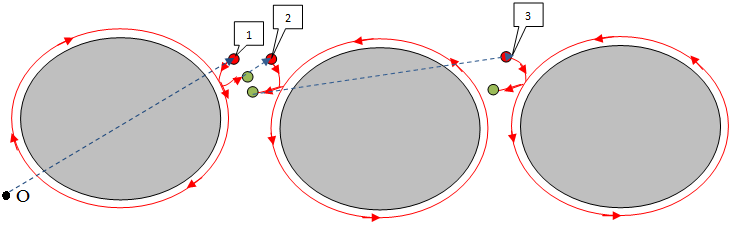
\includegraphics[width=0.9\textwidth]{3-3.png}
  \caption{Пример схемы резки трех круглых заготовок <<по замкнутому>> контуру}
  \label{3-3}
  \end{center}
\end{figure}

\begin{figure}
  \begin{center}
  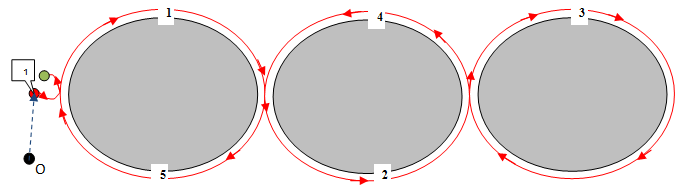
\includegraphics[width=0.9\textwidth]{3-1.png}
  \caption{Пример схемы резки трех круглых заготовок с применением специальной техники резки без дополнительного реза}
  \label{3-1}
  \end{center}
\end{figure}

На Рис. \ref{3-1}
цифрами от 1 до 5 показана последовательность
резки контуров за один сегмент,
т.е. после врезания в материал режущий инструмент
на рабочем ходу переходит к вырезке участка
под номером 1 первого контура,
затем без дополнительного реза режущая головка
переходит ко второму контуру и вырезает участок
контура под номером 2 и т.д.
В конце режущий инструмент завершает
вырезку трех контуров с одной точкой
врезки по пятому участку первого контура и
переходит к точке выключения.
Следует обратить внимание, что в рассматриваемом
способе резки инструмент переходит от одного контура к
другому на рабочем ходу без дополнительных резов,
за счет чего сокращаются значения основных параметров резки
$L_{on}, L_{off}, N_{pt}$.
Однако в результате применения предложенного метода
резки при обработке круглых заготовок в месте <<стыковки>>
контуров возможно образование <<ступеньки>>
(см. Рис. \ref{hiccup}),
что в некоторых случаях может привести к
искажению конечной геометрии и требуемых размеров заготовки.
Как показывает практика при обработке круглых заготовок на
машине лазерной листовой резки с ЧПУ размеры <<ступеньки>> незначительны
(достигают десятых-сотых долей мм)
и ее размеры либо попадают в требуемое поле допуска
для соответствующего размера, либо ее можно <<зачистить>>
с помощью дополнительной обработки без искажения геометрии и требуемых размеров.
Также следует отметить, что часто детали,
получаемые после лазерной обработки,
являются заготовками для дальнейших переделов с
припусками на требуемые размеры чертежа,
поэтому допускаются незначительные дефекты,
обработка которых в дальнейшем не приведет к
искажению требуемых размеров и форм конечной детали.

При размещении круглых заготовок в один ряд
либо вдоль оси Х, либо вдоль Y
возможно сокращение количества точек врезки до
$N_{pt}=1$
и сведение
$L_{off}$
к величине, равной нулю, если не считать перемещения
режущего инструмента на холостом ходу до точки врезки
для текущего ряда круглых заготовок и от точки выключения
режущего инструмента до следующей точки врезки или нулевой точки
($L_{off} \approx 0$).
В случае размещения круглых заготовок в $n$
рядов при использовании предложенного способа резки
$N_{pt}=n$.

\begin{figure}
  \begin{center}
  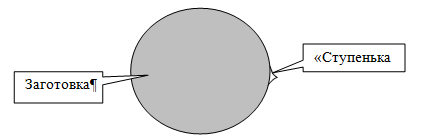
\includegraphics[width=0.7\textwidth]{hiccup.png}
  \caption{Возможная <<ступенька>> при обработке круглых заготовок с помощью специального метода резки}
  \label{hiccup}
  \end{center}
\end{figure}

Предложенный на рис. \ref{3-1}
метод резки круглых заготовок в основном применим для заготовок,
которые можно объединить в один блок и применить
данную специальную технику резки без дополнительного реза.
Однако на практике возникают случаи вырезки круглых заготовок
специальным способом с дополнительным резом
(рис. \ref{3-extra}).
Например, на производстве возникает задача
вырезки круглых заготовок разного габаритного размера,
а
также при построении маршрута перемещения режущего инструмента
на машинах термической резки с ЧПУ необходимо выполнение
технологических ограничений термической резки.
В частности, в случае необходимости выполнения условий
сокращения термических деформаций вырезку заготовок с
применением разработанной специальной техники резки
для круглых заготовок необходимо выполнять без изменения обхода контуров.
С этой целью может быть применим способ с дополнительным резом
(рис. \ref{3-extra})
во избежание повышения температуры в процессе резки контуров
в месте стыка деталей из-за острого угла
при переходе от одного контура к другому без изменения
направления обхода и во избежание образования <<ступеньки>>.
Вырезка контуров осуществляется аналогично способу,
приведенному выше (рис. \ref{3-3}),
однако при переходе от одного контура к другому
при необходимости возможен дополнительный рез
(при наличии деталей значительно отличающихся по размерам и смещении друг относительно друга).
В свою очередь это может привести к увеличению
$L_{on}$
на величину фактической длины дополнительных резов
$L_\text{доп}^\text{факт}$.
Поэтому в данном способе необходимо вычислять максимально допустимую длину дополнительного реза
$L_\text{доп}$
и
$L_\text{доп}^\text{факт} \leqslant L_\text{доп}$.
На рис. \ref{3-extra}
красными стрелками показан спроектированный путь
перемещения инструмента на рабочем ходу при прямом обходе контуров,
фиолетовым – обратный ход режущего инструмента
при завершении вырезки трех деталей с
применением специальной техники резки.

\begin{figure}
  \begin{center}
  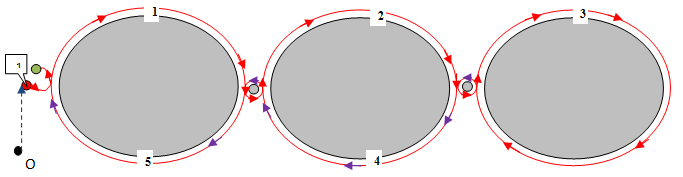
\includegraphics[width=0.9\textwidth]{3-extra.png}
  \caption{Пример схемы резки трех круглых заготовок с применением специальной техники резки с дополнительным резом}
  \label{3-extra}
  \end{center}
\end{figure}

Согласно предложенному методу режущая головка
после врезания в материал обходит по часовой
стрелки первый участок контура под номером 1,
после чего меняя направление обхода против
часовой стрелки совершает дополнительный рез и
переходит к вырезке участка под номером 2 второго
контура по часовой стрелке и т.д.
Пока режущий инструмент не завершит
вырезку полного контура с номером 3,
после чего режущая головка совершает обратный обход
оставшихся не вырезанных частей контуров под номерами 4 и 5.
Таким образом, можно вырезать заготовки разных размеров,
объединенных в блоки и внутри каждого блока реализовать
вырезку нескольких контуров с помощью одной точки врезки.
При этом дополнительный рез может быть выполнен по дуге,
либо по прямой в зависимости от размера внешнего контура заготовок.

С целью оценки эффективности в результате применения
разработанных специальных способов резки рассмотрим
пример резки круглых заготовок двумя вышеописанными
методами на машине лазерной листовой резки ByStar3015 с ЧПУ.
Для этого были разработаны две раскройные карты,
на которых были размещены 69 и 58 заготовок,
имеющих круглый наружный контур.

На рис. \ref{circles-a} и \ref{circles-b}
приведен маршрут резки
круглых заготовок одного размера без дополнительного реза,
на рис. \ref{circles-c} и \ref{circles-d} – с дополнительным резом.
Полученные результаты сравнивались с результатами
резки <<по замкнутому контуру>> и приведены в табл. 2.4.
Расчет был произведен для листового материала 12Х18Н10Т $\Delta$=1 и 5 мм.

\begin{figure}
  \begin{center}
  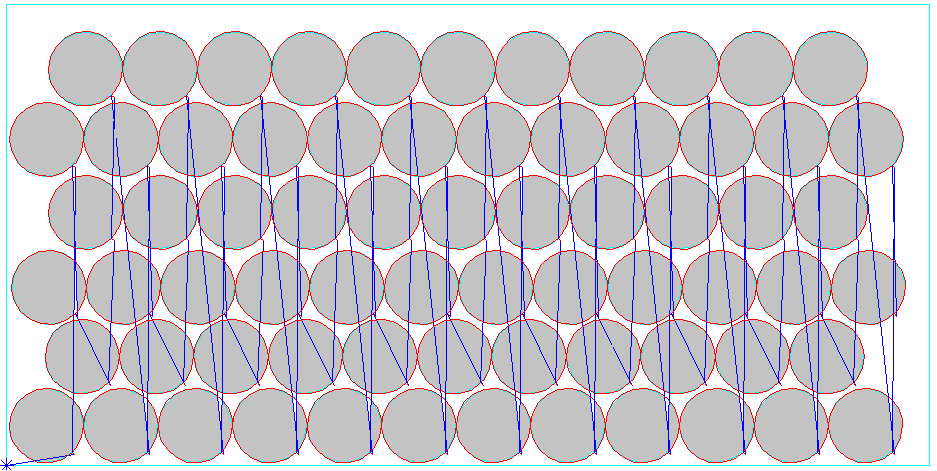
\includegraphics[width=0.9\textwidth]{circles-a.png}
  \caption{Пример маршрута резки круглых заготовок c применением резки <<по замкнутому контуру>>}
  \label{circles-a}
  \end{center}
\end{figure}

\begin{figure}
  \begin{center}
  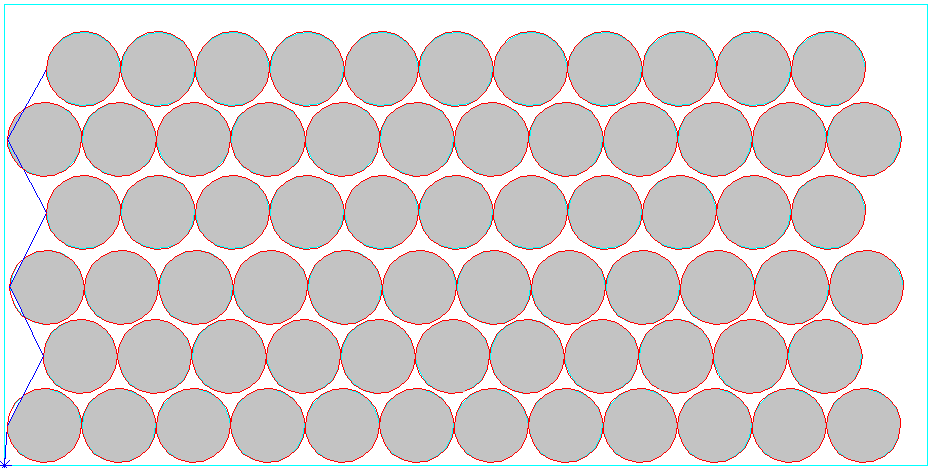
\includegraphics[width=0.9\textwidth]{circles-b.png}
  \caption{Пример маршрута резки круглых заготовок c применением метода резки без дополнительного реза}
  \label{circles-b}
  \end{center}
\end{figure}

На рис. \ref{circles-d}
разными цветами обозначены блоки деталей,
для которых реализована резка без дополнительного реза.
В частности, в нижней  части раскройной карты
может быть выделена
группа из 10 круглых заготовок и одного кольца.
Размеры заготовок отличаются незначительно,
поэтому есть возможность реализовать резку блока из 11 деталей с
помощью одной точки врезки и без дополнительного реза.
В  верхней части той же раскройной карте выделен блок из шести деталей,
вырезаемых с одной точкой врезки, при этом заготовки,
выделенные фиолетовым цветом, вырезаются без дополнительного реза,
но при переходе к серым заготовкам меньшего размера необходимо
вырезку осуществить с дополнительным резом.
При этом дальнейшая вырезка трех серых заготовок
осуществляется без дополнительного реза.

\begin{figure}
  \begin{center}
  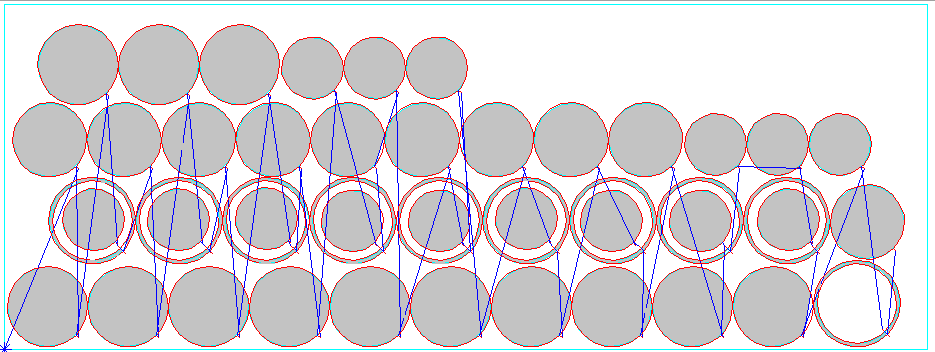
\includegraphics[width=0.9\textwidth]{circles-c.png}
  \caption{Пример маршрута резки круглых заготовок разного размера c применением резки <<по замкнутому контуру>>}
  \label{circles-c}
  \end{center}
\end{figure}

\begin{figure}
  \begin{center}
  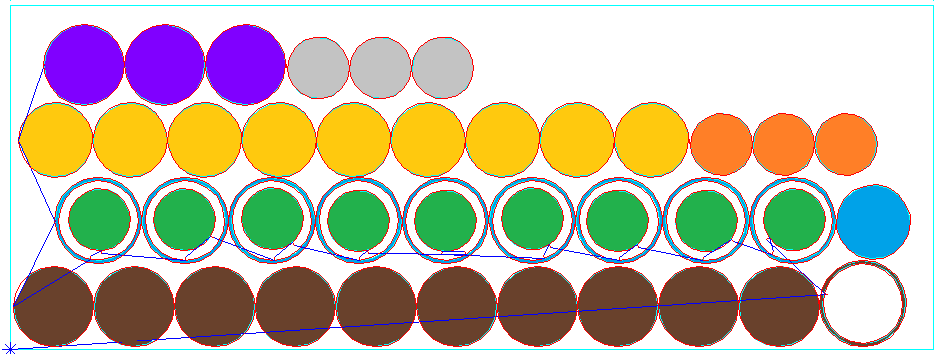
\includegraphics[width=0.9\textwidth]{circles-d.png}
  \caption{Пример маршрута резки круглых заготовок разного размера c применением специальной техники резки}
  \label{circles-d}
  \end{center}
\end{figure}

\begin{table}
  \caption{Результаты расчета стоимость резки раскройного плана для круглых заготовок с применением специальных способов резки}
  \label{circles}
  \centering
  \small
  \begin{tabular}{*{10}{c}}
    \hline
    Марка & $\Delta$ & Резка
      & \shortstack{$L_{on}$, \\ м}
      & \shortstack{$L_{off}$, \\ м}
      & $N_{pt}$
      & \shortstack{$F_{cost}$,\\ руб}
      & \%
      & \shortstack{$L_\text{доп}^\text{факт}$,\\ м} \\
    \hline
    \multirow{8}{*}{\rotatebox{90}{12Х18Н10Т}} & \multirow{4}{*}{1 мм} & Стандартная & 54,7 &	43,07	& 69 & 1552,92 & \multirow{2}{*}{15,6} &	\multirow{2}{*}{-} \\
    & & Без доп. реза & 52,02 &	0,7 & 6 & 1310,05 \\
    & & Стандартная   & 46,14 & 18,78 & 58 & 1302,08 & \multirow{2}{*}{6,88} & \multirow{2}{*}{0,16} \\
    & & С доп. резом  & 46,3  & 5,43  & 23 & 1212,43 \\
    & \multirow{4}{*}{5 мм} & Стандартная & 54,7 &	43,07	& 69 & 12154,8 & \multirow{2}{*}{14,3} &	\multirow{2}{*}{-} \\
    & & Без доп. реза & 52,02 &	0,7 & 6 & 10417,2 \\
    & & Стандартная   & 46,14 & 18,78 & 58 & 10241,6 & \multirow{2}{*}{6,2} & \multirow{2}{*}{0,16} \\
    & & С доп. резом  & 46,3  & 5,43  & 23 & 9607,08 \\
    \hline
  \end{tabular}
\end{table}

По результатам анализа приведенных в Табл. \ref{circles}
данных, можно сделать следующие выводы:

\begin{enumerate}
\item Применение специального метода резки круглых заготовок
без дополнительного реза (рис. \ref{circles-b})
приводит к сокращению количества точек врезок до 90\%
 и длины перемещений инструмента на холостом ходу до 98\%
 по сравнению с резкой по <<замкнутому контуру>>.
 При проведении ряда экспериментов в среднем значение $N_{pt}$
 сокращается на 60\%, значение $L_{off}$ на – 65\%.
 При этом стоимость обработки раскройной карты в среднем сокращается на 15\%;

\item Применение резки с дополнительным резом (рис. \ref{circles-d})
приводит в среднем к сокращению количества точек врезок на 60\%,
а длины перемещений инструмента на холостом ходу сокращается на 70\%
по сравнению с резкой <<по замкнутому контуру>>.
В свою очередь стоимость обработки сокращается на 7\%.
При этом следует отметить,
что по причине наличия внутренних контуров
наблюдается снижение эффективности применения
предложенных технологий;

\item В случае применения резки с дополнительным резом необходимо рассчитать
$L_\text{доп}^\text{факт}$.
и
$L_\text{доп}$
согласно (\ref{l-dop}) и (\ref{l-fact-dop}).
\end{enumerate}

\subsection{Стратегии проектирования маршрута режущего инструмента для многоугольных заготовок}

В машиностроительном производстве
при раскрое листового материала с помощью машин лазерной резки с ЧПУ
к наиболее часто встречающимся геометрическим
типам заготовок помимо круглых внешних контуров
относят также многоугольные заготовки,
часто выпуклые симметричные многоугольники с отверстиями различной формы.
В отдельную группу можно отнести треугольные и прямоугольные заготовки.
Следует отметить, что прямоугольные заготовки целесообразно обрабатывать
с помощью совмещенного реза.
Касательно остальных многоугольных (в т.ч. треугольных)
заготовок применение совмещенного реза не эффективно,
т.к. обычно с помощью одной точки врезки удается вырезать обычно две заготовки.
Также не эффективны другие специальные способы резки
(например, <<цепная>> резка или резка змейкой),
т.к. применение выделенных способов приводит к
сокращению количества точек врезок,
но
$L_{on}=const$
в лучшем случае или его увеличении,
что в свою очередь повышает время
$T_{cut}$
и стоимость раскроя
$F_{cost}$.
Поэтому возникает необходимость в разработке
новых специальных способов резки для выделенной группы заготовок.

В отдельную группу выделим треугольные заготовки,
для листовой резки которых на машине лазерной резки с ЧПУ
применим мультиконтурную резку,
совмещающую совмещенный рез и резку змейкой (рис.39).
На рис. \ref{6-6} приведена схема резки шести треугольных заготовок
одного размера с помощью резки <<по замкнутому>> контуру при этом
$N_{pt}=6$,
цифрами 1-6 обозначена последовательность резки.
На рис. \ref{6-1} приведена схема резки тех же шести
треугольных заготовок, при этом
$N_{pt}=1$.

\begin{figure}
  \begin{center}
  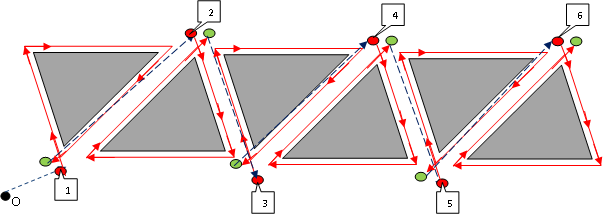
\includegraphics[width=0.9\textwidth]{6-6.png}
  \caption{Схема резки шести треугольных заготовок с помощью резки <<по замкнутому контуру>>}
  \label{6-6}
  \end{center}
\end{figure}

\begin{figure}
  \begin{center}
  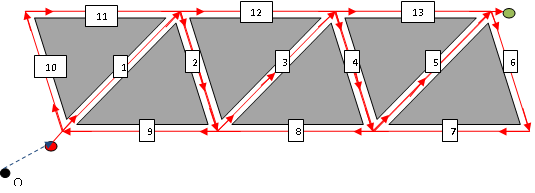
\includegraphics[width=0.9\textwidth]{6-1.png}
  \caption{Схема резки шести треугольных заготовок с помощью специального способа резки}
  \label{6-1}
  \end{center}
\end{figure}

Здесь цифрами 1-13 обозначена последовательность
резки контуров в одном сегменте,
т.е. после врезания в материал режущий инструмент
на рабочем ходу переходит к вырезке участка под номером 1
первого контура,
затем без дополнительного реза режущая головка
переходит ко второму контуру и вырезает участок под номером 2 и т.д.
В конце режущий инструмент завершает вырезку шести контуров
с одной точкой врезки по 13 участку и переходит к
точке выключения инструмента.
Следует обратить внимание, что в рассматриваемом способе
резки инструмент переходит от одного контура к другому
на рабочем ходу с совмещенным резом,
за счет чего сокращается количество точек врезок $N_{pt}$,
расстояние перемещений инструмента на рабочем $L_{on}$
и холостом  $L_{off}$ ходах.

Способ резки, предложенный на рис. \ref{6-1},
применим для групп треугольных заготовок одного типоразмера,
расположенных в два ряда.
При этом если количество рядов больше двух,
то создаются еще блоки заготовок,
каждый из которых включает в себя по 2 ряда треугольных заготовок.
Переход режущего инструмента от одного блока к другому
осуществляется с помощью холостого хода.
Внутри каждого блока реализована резка заготовок с одной точкой врезки.

В случае раскроя листового материала треугольными
заготовками можно спроектировать маршрут режущего
инструмента без холостого хода,
для этого треугольные заготовки необходимо
размещать согласно рис. \ref{3-10}.
Основное условие непрерывной резки нескольких
заготовок заключается в том,
что общее количество пересекающихся ребер у
любой вершины треугольника должно быть четным.
Или, с точки зрения теории графов,
у каждой вершины
должно быть четное количество ребер.
В обратном случае непрерывную резку заготовок
с помощью одной точки врезки не осуществить
без дополнительных резов.
Например, как видно из рис. \ref{3-10}
общее количество обозначенных цифрами 1,2,4,5,7 и 8 ребер равно 6.

Цифрами 1-18 обозначена последовательность
резки контуров за один сегмент,
т.е. после врезания в материал режущий инструмент
на рабочем ходу переходит к вырезке участка
под номером 1 первого контура,
затем без дополнительного реза режущая
головка переходит ко второму контуру и
вырезает участок под номером 2 и т.д.
В конце режущий инструмент завершает
вырезку девяти контуров с одной точкой врезки
по 18 участку и переходит к точке выключения инструмента.
Следует обратить внимание, что в рассматриваемом способе
резки инструмент переходит от одного контура к
другому на рабочем ходу с совмещенным резом,
за счет чего сокращается количество точек врезки $N_{pt}$,
расстояние перемещений инструмента на рабочем ходу  $L_{on}$,
при этом
$L_{off} \approx 0$.
Холостой переход осуществляется
только при переходе режущего инструмента
от нулевой точки до точки врезки и от
точки выключения инструмента до нулевой точки.
Способом, приведенным на рис. \ref{3-10},
можно размещать большое количество
треугольных заготовок, при этом всегда $N_{pt}=1$
и $L_{off} \approx 0$.

\begin{figure}
  \begin{center}
  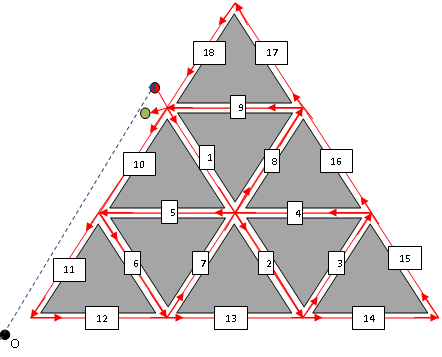
\includegraphics[width=0.8\textwidth]{3-10.png}
  \caption{Схема резки девяти треугольных заготовок с помощью мультиконтурной резки}
  \label{3-10}
  \end{center}
\end{figure}

Предложенные выше методы резки  применимы для любых треугольников.

Обработку пятиугольных заготовок из листового материала
на машине лазерной резки с ЧПУ также можно осуществить
предложенным методом, приведенным на рис. \ref{6-1}
с помощью мультиконтурной резки,
объединяющей совмещенный рез и резку змейкой.
На рис. \ref{5-6}
приведена схема резки <<по замкнутому>> контуру
шести пятиугольных заготовок;
при этом $N_{pt}=6$.

\begin{figure}
  \begin{center}
  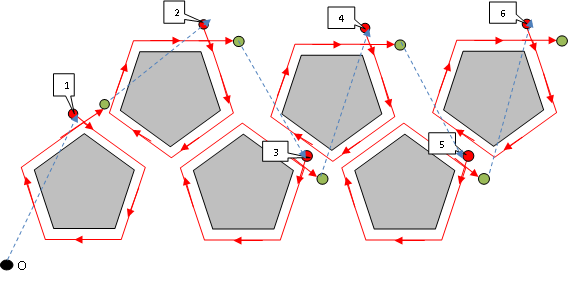
\includegraphics[width=0.9\textwidth]{5-6.png}
  \caption{Схема резки <<по замкнутому контуру>> шести пятиугольных заготовок}
  \label{5-6}
  \end{center}
\end{figure}

На рис.\ref{5-1}
предложена схема резки тех же шести
пятиугольных заготовок за один сегмент, при этом  $N_{pt}=1$
и $L_{off} \approx 0$.

\begin{figure}
  \begin{center}
  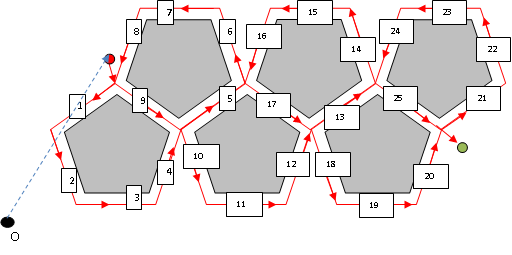
\includegraphics[width=0.9\textwidth]{5-1.png}
  \caption{Схема резки шести пятиугольных заготовок
  с применением мультиконтурной резки}
  \label{5-1}
  \end{center}
\end{figure}

С помощью схемы, приведенной на рис. \ref{5-1},
можно осуществлять резку по ребрам многоугольников,
соблюдая последовательность и направление резки каждого ребра.
Инструмент перемещается на холостом ходу от
начальной точки положения инструмента
(точки О)
до точки врезки, после чего осуществляется непрерывная резка всех ребер,
начиная с 1, без дополнительных резов за один сегмент.
После того как режущий инструмент частично вырежет
первый контур по 4 ребрам (с 1 по 4)
переходит к 5 ребру и начинает вырезать
второй контур последовательно вырезая с 6 по 9 ребра.
При вырезке 9 ребра будут окончательно
вырезаны первый и второй контура.
Аналогично можно вырезать оставшиеся контура,
после чего инструмент переходит в точку выключения инструмента.
Как видно из рис. \ref{5-1},
за счет применения совмещенного реза сокращается $L_{on}$,
за счет отсутствия холостых переходов
$L_{off} \approx 0$
и $N_{pt}=1$
при одновременном сокращении общего времени
и стоимости резки заготовок из листового
материала на машинах лазерной резки с ЧПУ.
Предложенный способ резки применим для любых выпуклых пятиугольников.

В случае обработки четырехугольных заготовок
целесообразно применять совмещенный рез,
либо технологию, предложенную на рис. \ref{5-1},
при условии, что общее количество ребер,
пересекающихся в любой внутренней вершине, будет четным.
В последнем случае по сравнению с совмещенным резом значения
$N_{pt}$
и $L_{off}$
при использовании разработанного способа резки будут,
как правило, ниже, чем при совмещенном резе.
Но данный способ резки не всегда применим
с точки зрения снижения КИМ.

В общем случае при резке любых многоугольных
заготовок для случая,
когда количество пересекающихся ребер у вершин
(в частности внутренних) нечетно,
то предложенный способ резки реализуем с
дополнительным резом, либо с добавлением точек врезки.
Следует обратить внимание на то,
что при мультиконтурной резке многоугольников с
дополнительным резом, значение
$L_\text{доп}^\text{факт}$.
также как и для треугольников должно удовлетворять условию
$L_\text{доп}^\text{факт} \leqslant L_\text{доп}$,
рассчитанному по (\ref{l-fact-dop}),
а иначе значения целевых функций (\ref{cutting-time})
и (\ref{cutting-cost})
окажутся больше значений,
получаемых  при резке <<по замкнутому контуру>>.
На рис. \ref{5-extra}
для любой вершины количество пересекающихся ребер нечетно,
поэтому резка контуров возможна только с дополнительным резом.
Цифрами 1-19 обозначена последовательность обхода ребер
пяти заготовок.
Режущий инструмент на холостом ходу переходит
из начальной точки в точку врезки,
после чего по эквидистантому контуру
осуществляется частичная вырезка первого
контура по ребрам 1-4,
затем вырезается ребро 5 второй заготовки и т.д.
пока окончательно не будут вырезаны пять заготовок по ребрам 6-19.
По причине наличия дополнительных резов рабочая
длина перемещения режущего инструмента может увеличиться по сравнению с $L_{on}$,
полученной в результате применения резки <<по замкнутому контуру>>,
поэтому актуален вопрос проверки неравенства
$L_\text{доп}^\text{факт} \leqslant L_\text{доп}$.
В результате применения предложенного на рис. \ref{5-extra}
специального метода резки
$N_{pt}=1$
и $L_{off} \approx 0$.

\begin{figure}
  \begin{center}
  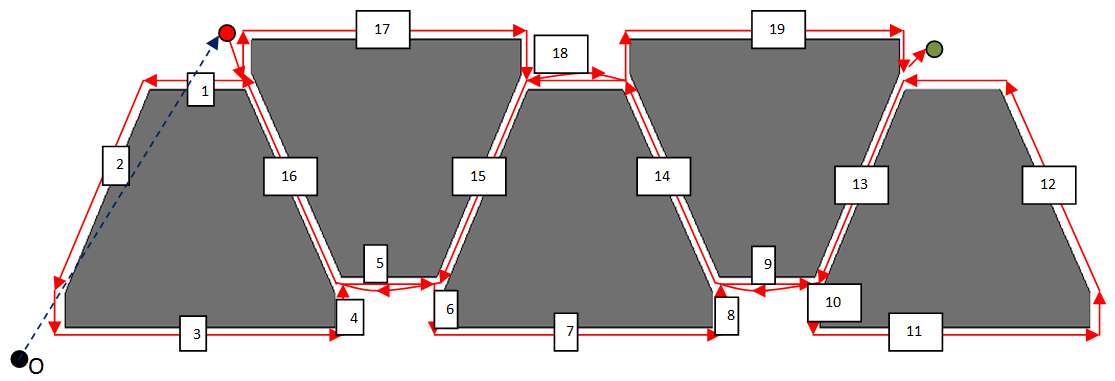
\includegraphics[width=0.9\textwidth]{5-extra.png}
  \caption{Схема резки пяти заготовок с помощью мультиконтурной резки с дополнительным резом}
  \label{5-extra}
  \end{center}
\end{figure}

Рассмотрим пример раскроя листового материала
12Х18Н10Т ($\Delta$=1-8мм)
многоугольными заготовками на машине лазерной резки с ЧПУ.
Для этого разработаны две раскройные карты с одинаковым количеством,
видом и размерами деталей,
для которых спроектирован маршрут перемещения
режущего инструмента в САПР <<СИРИУС>> с
применением резки <<по замкнутому контуру>> (рис. \ref{multi-a})
и специальной техники резки для многоугольных заготовок (рис.45).
Полученные результаты, которые содержат значения
$L_{on}$, $N_{pt}$, $L_{off}$, $T_{cut}$ и $F_{cost}$
для каждой раскройной карты, приведены в Таблице 5.

\begin{figure}
  \begin{center}
  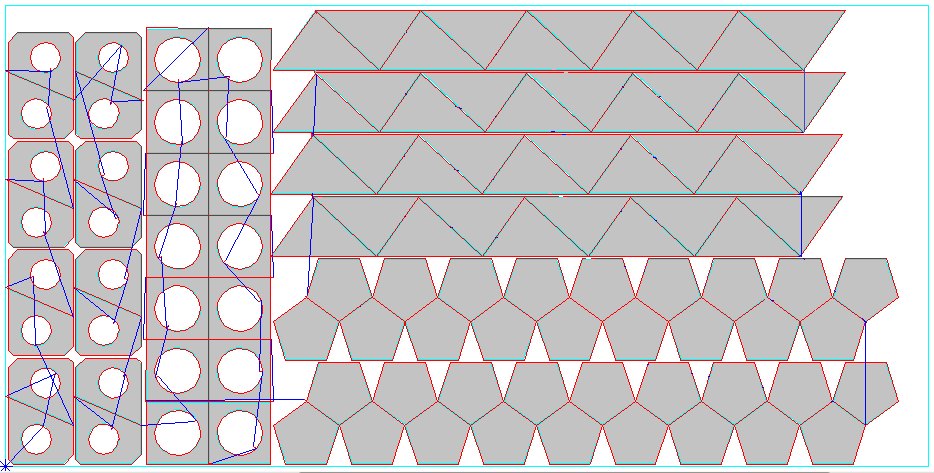
\includegraphics[width=0.9\textwidth]{multi-a.png}
  \caption{Схема раскройной карты с применением мультиконтурной резки для многоугольных заготовок}
  \label{multi-a}
  \end{center}
\end{figure}

\begin{figure}
  \begin{center}
  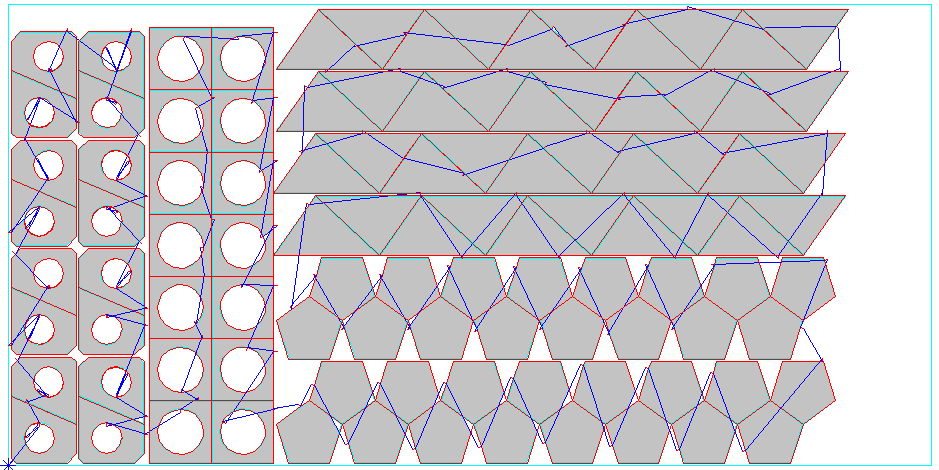
\includegraphics[width=0.9\textwidth]{multi-b.png}
  \caption{Схема раскройной карты с применением резки <<по замкнутому контуру>>}
  \label{multi-b}
  \end{center}
\end{figure}

Применение предложенных специальных методов резки
приводит к значительному сокращению значений
$N_{pt}$, $L_{on}$ и $L_{off}$
в сравнении со стандартной техникой резки
соответственно до 70\%, 27\% и 67\%
при одновременном сокращении времени
$T_{cut}$
и стоимости лазерной резки
$F_{cost}$ до 36\%.
Как показывает практика применения
предложенных методов резки при проектировании
УП в реальном производственном процессе,
в среднем значения параметров
$L_{on}$, $N_{pt}$  и $L_{off}$
сокращаются на 3\%, 60\% и 65\%
соответственно при одновременном снижении
$F_{cost}$
на 10-20\%
по сравнению с резкой <<по замкнутому контуру>>.
Как видно из табл. \ref{polygons},
с увеличением толщины обрабатываемого материала
сокращается эффективность предложенных специальных способов резки.

\begin{table}
  \caption{Результаты расчета стоимости резки раскройного плана
    для многоугольных заготовок}
  \label{polygons}
  \centering
  \begin{tabular}{*{8}{c}}
    \hline
    Марка & $\Delta$ & Резка &
      \shortstack{$L_{on}$, \\ м} &
      \shortstack{$L_{off}$, \\ м} &
      $N_{pt}$ &
      \shortstack{$F_{cost}$, \\ руб} &
      \% \\
    \hline
    \multirow{2}{*}{12Х18Н10Т} & \multirow{2}{*}{1 мм} & Стандартная & 101,85 & 26,92 & 163 & 2956,14 & \multirow{2}{*}{36} \\
    & & Специальная & 74,73 & 8,9 & 51 & 1901,4 \\
    \multirow{2}{*}{12Х18Н10Т} & \multirow{2}{*}{3 мм} & Стандартная & 101,85 &	26,92 & 163 & 9170,09 & \multirow{2}{*}{36.5} \\
    & & Специальная & 74,73 & 8,9 & 51 & 5823,10 \\
    \multirow{2}{*}{12Х18Н10Т} & \multirow{2}{*}{5 мм} & Стандартная & 101,85 & 26,92 & 163 & 23262,44 & \multirow{2}{*}{32.2} \\
    & & Специальная & 74,73 & 8,9 & 51 & 15768,17 \\
    \multirow{2}{*}{12Х18Н10Т} & \multirow{2}{*}{8 мм} & Стандартная & 101,85 & 26,92 & 163 & 94070,86 & \multirow{2}{*}{29.7} \\
    & & Специальная & 74,73 & 8,9 & 51 & 66121,93 \\
  \end{tabular}
\end{table}

Выводы:

\begin{enumerate}
\item Применение специальных методов резки
для различных многоугольных заготовок возможно
без дополнительных резов между заготовками при условии,
что количество пересекающихся ребер у вершин
(в частности внутренних) четно.
В остальных случаях резка разработанным
способом резки возможна с дополнительным резом,
либо с увеличением числа точек врезок.
Предложенные методы базируются на известных методах резки
(змейкой и совмещенный рез),
за счет этого значительно сокращаются
значения основных параметры
$L_{on}$, $N_{pt}$  и $L_{off}$
и   при одновременном снижении
$T_{cut}$
и
$F_{cost}$;

\item В зависимости от типа заготовок,
наличия или отсутствия отверстий в деталях
количество точек врезки может снизиться до
$N_{pt}=1$,
при этом
$L_{off} \approx 0$.
В рассмотренных примерах значения
$N_{pt}$, $L_{off}$ и $L_{on}$
иаксимально сокращаются соответственно до 70\%, 67\% и до 27\%
при одновременном сокращении
$T_{cut}$
и
$F_{cost}$
до 36\%.
В среднем значение $F_{cost}$ снижается на 10-20\%;

\item При применении предложенных специального способа резки
для многоугольных деталей с дополнительным резом
необходимо вычислять значение
$L_\text{доп}^\text{факт}$:
$L_\text{доп}^\text{факт} \leqslant L_\text{доп}$.
В противном случае значение
$L_\text{доп}$.
может оказаться больше значения
$L_{on}$,
полученное при резке <<по замкнутому контуру>>,
что в свою очередь может привести к увеличению значений целевых функций
$T_{cut}$
и
$F_{cost}$.

\item Эффективность от применения предложенных способов резки
сокращается при увеличении толщины обрабатываемого материала.
\end{enumerate}

{\bf Заключительные замечания}

Предложенные способы применения специальных техник резки и
формирование групп однотипных заготовок на этапе
проектирования раскроя листовых материалов на фигурные заготовки,
среди которых присутствуют круглые и многоугольные,
можно интерпретировать как методы формирования наборов базовых сегментов
(а в дискретном случае – мегаполисов)
для последующего решения задач оптимизации класса GSCCP
средней и большой размерности.
Это создает, в свою очередь,
предпосылки  для разработки эффективных методов
решения интегрированной задачи раскроя и мсаршрутизации,
для которой целевая функция стоимости складывается
из стоимости использованного материала для раскроя
и стомости процесса резки
$
F_{cost}=
L_{on} \cdot C_{on} +
L_{off} \cdot C_{off} +
N_{pt} \cdot C_{pt}
$.

\section{Разработка методов учета динамических ограничений
  в оптимизационных алгоритмах маршрутизации инструмента машин для термической резки листовых заготовок}

Как отмечалось в параграе 1.3.
%%% TODO fix reference ^^^^^^^^^^^^^
наиболее сложной проблемой при разработке методов оптимизации
траектории инструмента машин листовой резки с ЧПУ
является математическая формализация и
разработка вычислительных алгоритмов учета
технологических эвристических требований термической резки,
т.н. правил <<жесткости детали>>и <<жесткости листа>>.
<<Динамический>> характер этих условий, заключающийся в том,
что сами ограничения формируются только в процессе вычисления
допустимого решения задачи, по сути порождает
новый не исследованный ранее класс маршрутных задач
с крайне сложными видами ограничений типа (1.3.5).

Ниже приведен способ формализациии правила <<жесткости детали>>,
основанный на введении понятия <<зона жесткости>>.

{\it Определение 5}.
Зоной жесткости называется область,
ограниченная следующими четырьмя геометрическими кривыми:
1)траекторией инструмента;
2)эквидистантной этой траектории кривой, отстоящей на величину $R$;
3)прямой, проходящей через точку выключения инструмента $M^*$
перпендикулярно траектории инструмента в этой точке;
4) прямой, проходящей через точку,
отстоящую от точки выключения инструмента $M^*$ на некоторую величину $L$,
перпендикулярно траектории инструмента в этой точке.

Параметры этой зоны для двух точек
(длина $L$ и радиус $R$)
определяются в каждом конкретном случае
на основании эксперной оценки,
зависящей, в частности, от марки и толщины материала,
а также технологии термической резки.
На Рис. \ref{hardness-area}
эти зоны выделены желтым цветом.

\begin{figure}
 \begin{center}
  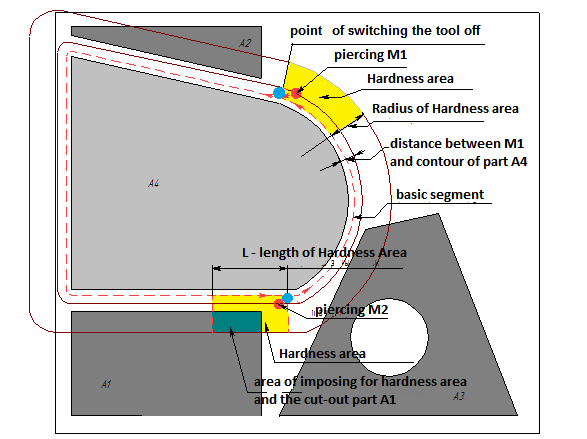
\includegraphics[width=0.9\textwidth]{hardness-area.png}
  \caption{Формализация правила <<жесткости детали>> на основе понятия <<зоны жесткости>>}
  \label{hardness-area}
  \end{center}
\end{figure}

Тогда в оптимизационных процедурах машрутизации
для задачи GTSP  и дискретных моделей задач CCP, SCCP, GSCCP
выбор точки врезки M и точки выключения инструмента $M^*$
(сегмента резки) определяется простым условием:
{\bf зона жесткости} должна лежать в еще невырезанной
<<жесткой>> части листового материала.
Для тех точек врезки, для которых это условие не выполнено,
значение целевых функций  увеличивается на некоторую величину <<штрафа>>.

Как нетрудно видеть,
сформулированное правило выбора <<хороших>> точек врезки
и точек выключения инструмента носит геометрический характер.
Поскольку технологическое правило <<жесткости>> детали
связано с тепловыми деформациями материала,
то естественно предположить,
что температура в <<хороших>> зонах <<жесткости>> будет меньше,
чем в <<плохих>>.
В случае справедливости этой гипотезы,
адекватная оценка тепловых деформаций материала
при термической резке заготовок на машинах с ЧПУ
может иметь важное значение как инструмент
обеспечения необходимых технологических требований.
Для проверки гипотезы необходимо иметь инструментарий
моделирования и вычисления температуры тепловых полей в
каждый момент времени процесса резки.
Для разработки необходимого программного
обеспечения рассмотрим следующую задачу.

{\bf Постановка задачи}

Имеется металлическая пластина.
Заданы контуры, последовательность их резки,
точки врезки и направления обходов.
Для режущего инструмента заданы <<радиус теплового луча>>,
мощность, скорость перемещения и скорость холостого хода.
Требуется рассчитать тепловые поля при
последовательной резке контуров.

{\bf Расчет процесса резки контуров}

Последовательно для каждого контура рассматривается задача нахождения
$\theta(t, x)$ - температуры
($t$ -момент времени,
$x$ - точка области), удовлетворяющей уравнению теплопроводности
\begin{equation}
c \rho \frac{\partial \theta}{\partial t}=k \Delta \theta +N, x \in \Omega
\end{equation}
начальному условию
\begin{equation}
  \theta(t_0, x)=\theta_0(x), x \in \Omega
\end{equation}
граничному условию
\begin{equation}
  -k \frac{\partial \theta}{\partial n}=M(\theta - \theta_*), x \in \partial \Omega
\end{equation}
$t$ из промежутка $[t_0, t_1]$,
$x$ - точка области
$\Omega \subset \mathbb R^3$.

Здесь
$t_0$ - время начала и
$t_1$  - время окончания резки текущего контура,
$\Omega$ - часть пластины, которая осталась после удаления областей,
ограниченных предыдущими контурами,
$\partial \Omega$ - граница области $\Omega$.
$c$ – удельная массовая теплоемкость,
$\rho$ – плотность,
$k$ – коэффициент теплопроводности,
$N(t,x)$ – плотность тепловых источников,
$M$ - коэффициент теплопередачи,
$\theta_0(x)$ - текущее температурное поле перед началом резки данного контура,
$\theta_*$ -температура воздуха.

Функция $N$ плотности тепловых источников имеет следующий вид.
Пусть толщина листа  $h$,
<<радиус теплового луча>> $r$,
его мощность w и скорость перемещения $v$.
Пусть  $m(t)$ – положение оси теплового <<луча>> в момент $t$.
Тогда
$p=w/(\pi r^2 h)$
есть
плотность мощности теплового <<луча>> и
$N(t,x)=p$
в точках, находящихся от прямой $m(t)$
на расстоянии меньше $r$  и
$0$ в остальных точках.

{\bf Аппроксимация задачи}

Процесс пересчета температурного поля
$\theta(t, x)$
во время резки контура
разбивается на малые промежутки времени
$[t_{r-1}, t_r]$
длины  $\Delta t$
и для расчета
$\theta(x)=\theta(t_r, x)$
рассматривается задача

\begin{equation}
c \rho \frac{\theta(x)-\theta_0(x)}{\Delta t}=k \Delta \theta(x) + N(X)
\end{equation}
\begin{equation}
  -k \frac{\partial \theta}{\partial n}=M(\theta - \theta_*)
\end{equation}
где
$\theta_0=\theta(t_{r-1}, x)$
и
$N(x)=N(t_{r-1},x)$.

Область
$\Omega$
разбивается на тетраэдры,
функции
$\theta(x), \theta_0(x), N(x)$ - кусочно-линейные,
определяемые значениями в узлах – вершинах тетраэдров.
Решение данной задачи является точкой минимума следующего функционала

\begin{multline}
  I(\theta) =
  \frac{1}{2 \Delta t} \int\displaylimits_\Omega c \rho (\theta - \theta_0)^2 dx
  + \frac12 \int\displaylimits_\Omega k |\nabla \theta|^2 dx \\
  - \int\displaylimits_\Omega N \theta dx
  + \frac12 \int\displaylimits_{\partial \Omega} M(\theta - \theta_*)^2 dS
\end{multline}

Нахождение точки минимума данного квадратичного фунционала
проводится методом релаксации.
Выбор метода основан на следующих соображениях.

Так как радиус  $r$
<<теплового луча>> мал,
то тетраэдры разбиения области должны иметь малый размер
(в расчетах длина сторона была  2 мм)
и поэтому их много.
В узлах, далеких от точек где уже был <<тепловой луч>>
и куда еще не могло дойти изменение тепла к данному моменту времени,
температура остается первоначальной.
Метод релаксации позволяет пропустить такие узлы,
что позволяет уменьшить время счета.

{\bf Замечание}.
Для уменьшения числа тетраэдров (узлов)
при расчете резки очередного контура
$K_i$
рассматривается не вся оставшаяся пластина, а кусок
$\Omega_i \supset \Omega_{i-1}$.
Кусок  достаточно большой,
чтобы к моменту завершения резки контура
$K_i$
температура вне
$\Omega_i$
не могла измениться.
После завершения резки контура
тетраэдры внутри контура удаляются и их число уменьшается.
Дальше производится расширение СКЭ до следующего куска
$\Omega_{i+1}$.

{\bf Просмотр результатов}

Разработанное программное обеспечени
позволяет просматривать изменение температурных полей
в процессе резки.
На рис. \ref{thermal-plan}
показан пример задания порядка резки
6-ти заготовок (8 контуров),
точек врезки и направление обхода
(минус означает обход по часовой стрелке).
Материал пластины -  сталь 12Х2Н4А,
толщина $h$ = 2 мм, размеры 1000 $\times$ 1000 мм.
Радиус <<теплового луча>> $r$ = 2 мм,
мощность $w$ = 1000 вт,
скорость $v$ = 10 м/с.

На рис. \ref{thermal-5} показано температурное поле
на одной из стадий процесса резки 5-го контура.

{\bf Замечание}.
Рисунки \ref{thrm-high} и \ref{thrm-low}  иллюстрирую справедливость гипотезы.
Эти процессы отличаются только выбором точкой врезки.
На рис. \ref{thrm-high} точка врезки вблизи кромки пластины.
Средняя температура в выделенном окне
вокруг точки завершения резки контура 480$^o$С.
На рис. \ref{thrm-low} точка врезки далеко от кромки.
Средняя температура в выделенном окне  362$^o$С.

\begin{figure}
  \centering
  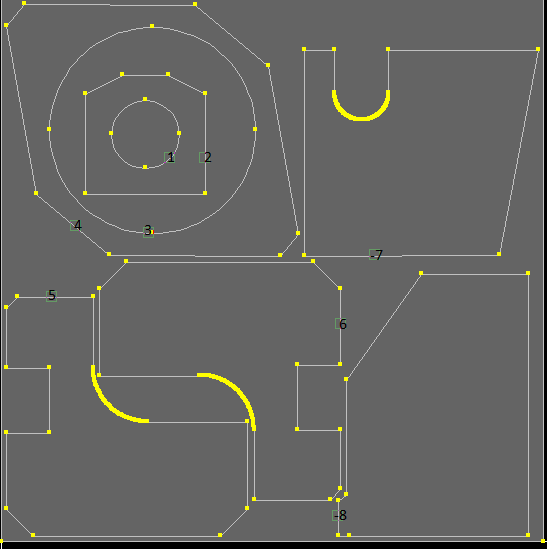
\includegraphics[width=0.6\textwidth]{thermal-plan.png}
  \caption{Места точек врезки и порядок резки для 8-ми контуров}
  \label{thermal-plan}
\end{figure}

\begin{figure}
  \centering
  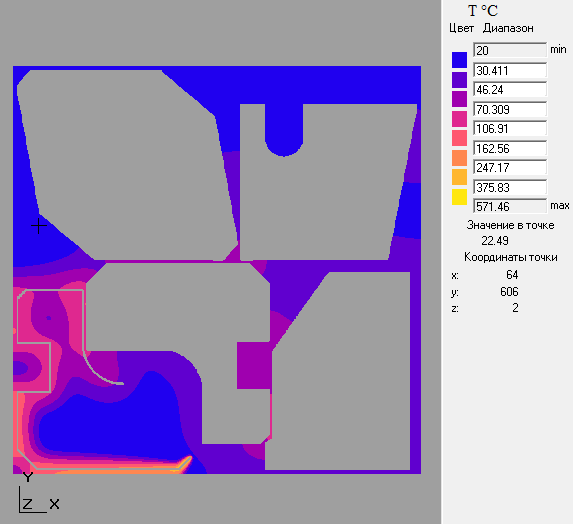
\includegraphics[width=0.7\textwidth]{thermal-5.png}
  \caption{Пример распределения тепловых полей в процессе резки 5-го контура}
  \label{thermal-5}
\end{figure}

\begin{figure}
  \centering
  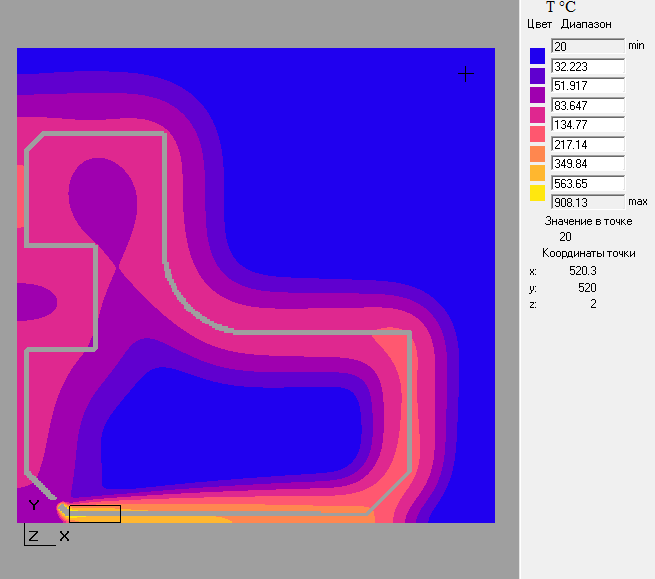
\includegraphics[width=0.6\textwidth]{thermal-high.png}
  \caption{Температурное поле при выборе точки врезки вблизи края пластины}
  \label{thrm-high}
\end{figure}

\begin{figure}
  \centering
  \includegraphics[width=0.6\textwidth]{thermal-low.png}
  \caption{Температурное поле при выборе точки врезки вдали от края пластины и границ вырезанных заготовок}
  \label{thrm-low}
\end{figure}

Другие проведенные вычислительные эксперименты
также показали уменьшение температуры материала
в <<хороших>> зонах в среднем на 63\%.
Ниже приведены еще два примера расчета температурных полей.

\begin{figure}
  \centering
  \subfigure[309 градусов Цельсия (точка выключения инструмента не удовлетворят правилу <<жесткости детали>>) ]{
    \includegraphics[width=0.9\textwidth]{thermal-309.png}
    \label{thermal-309}
  }
  \subfigure[120 градусов (точка выключения удовлетворят данному правилу)]{
    \includegraphics[width=0.9\textwidth]{thermal-120.png}
    \label{thermal-120}
  }
  \caption{Уменьшение температуры металла в зоне жесткости }
  \label{thermal-309-120}
\end{figure}

Таким образом,
анализ температурных полей подтверждает
геометрические правила выбора точек врезки
и точек выключения инструмента машин термической
резки материала и в будущем
(при условии разработки быстродействующих систем температурного анализа)
может сам служить средством для выбора точек начала и конца сегментов резки.

\begin{figure}
  \centering
  \subfigure[550 градусов]{
    \includegraphics[width=0.9\textwidth]{thermal-550.png}
    \label{thermal-550}
  }
  \subfigure[130 градусов]{
    \includegraphics[width=0.9\textwidth]{thermal-130.png}
    \label{thermal-130}
  }
  \caption{Уменьшение температуры металла в зоне жесткости }
  \label{thermal-550-130}
\end{figure}



Рассмотрим далее один из простых способ учета правила жесткости листа,
описанного в параграфе 1.3,
основанный на делении области листа на
последовательный набор подобластей (зон) (1.3.3):
$$
B_j =
\bigcup_{r=1}^l \Omega_r
$$

Способ заключается в том,
что после определения направления вырезки деталей на листе
(например, слева направо),
область листа разбивается вертикальными линиями
на прямоугольники одинакового размера.
Количество прямоугольников $l$
варьируется от 4 до 10 в зависимости от
геометрических размеров деталей
(чем крупнее размеры прямоугольников,
тем меньше формируется число зон).
Затем в каждой зоне решается основная задача (\ref{problem-statement})
уже без учета требований жесткости листа,
но с учетом правила <<жесткости детали>>
с помощью  алгоритма, описанного выше в этом параграфе.

На Рис.\ref{zones-a}
приведен пример оптимизации траектории
инструмента для задачи GTSP с учетом
формирования подобластей  (1.3.3).
Число подобластей в данном примере – 5.

\begin{figure}
  \begin{center}
  \includegraphics[width=0.9\textwidth]{zones-a.png}
  \caption{Пример моделирования траектории инструмента машины листовой резки с ЧПУ
    с учетом правила <<жесткости листа>> и с использованием зон (20 контуров, задача GTSP)}
  \label{zones-a}
  \end{center}
\end{figure}

На Рис. \ref{zones-b}
эта же задача решена без учета
<<динамических>> ограничений
(и правила жесткости детали и правила жесткости листа).
Ограничения на координаты точек врезки и
точки выключения инструмента,
обусловленные деформацией материала при врезке и
условия предшествования были соблюдены.
В качестве оптимизационного алгоритма
использован метод динамического программирования,
т.е. решение является глобальным экстремумом.
При этом для этого решения в маршруте резки
длина холостого хода инструмента уменьшилась на 26\%.

\begin{figure}
  \begin{center}
  \includegraphics[width=0.9\textwidth]{zones-b.png}
  \caption{Схема оптимального маршрута резки для примера на Рис. \ref{zones-a}}
  \label{zones-b}
  \end{center}
\end{figure}


{\bf Заключительные замечания}

Описанные в данном параграфе практические методы учета
правил жесткости детали и жесткости листа позволяют
имплементировать их в существующие оптимизационные
алгоритмы решения задачи (\ref{problem-statement})
с целевыми функциями \ref{cutting-time} - \ref{cutting-cost}
и получать рациональные варианты маршрута резки,
уменьшающие геометрические искажения деталей
при термической резке для большинства практических задач.
Вместе с тем, следует отметить,
что описанные способы в некоторых случаях не гарантируют 100\%
соблюдения технологических требований и
приводят к существенным тепловым деформациям материала.
Помимо этого остается открытым вопрос о разработке
эффективных алгоритмов получения глобальных экстремумов или
близких к ним для решения задач большой размерности с
одновременным учетом всех технологических требований
термической резки, включая динамические ограничения.
Этот вопрос  пока еще ждет своего решения.













%Part2
\part{Математические модели и методы решения задач маршрутизации, связанных с листовой резкой на машинах с ЧПУ.}
%Часть II. Математические модели и методы решения задач %маршрутизации, связанных с листовой резкой на машинах с ЧПУ.

\section*{Предварительные замечания по математическим методам маршрутизации инструмента машин листовой резки с ЧПУ}

Как видно из построений двух предыдущих глав, образующих первую часть монографии, инженерные задачи, связанные с управлением инструментом при листовой резке на машинах с ЧПУ, являются очень сложными и, в ряде случаев, плохо формализуемыми. С точки зрения идей, используемых в дискретной оптимизации, они существенно отличаются не только в количественном, но и в качественном отношениях от своего естественного прототипа – задачи коммивояжера (ЗК) или TSP (в англоязычной литературе). Прежде всего эти отличия связаны с наличием большого числа разнообразных ограничений, обусловленных технологическими требованиями. Исследование вышеупомянутых инженерных задач требует построения специализированной математической теории. Данная теория, как представляется, может рассматриваться как ветвь теории управления с дискретным временем. Вполне естественным представляется поэтому широкое использование аппарата динамического программирования (ДП) при должной формализации основных элементов содержательной постановки первой части.

Отметим прежде всего, что в процессе последовательного управления режущим инструментом объектами посещения являются не <<города>> (как в ЗК), а мегаполисы, получающиеся в свою очередь дискретизацией эквидистант контуров, подлежащих резке. Сама эта дискретизация нужна для последующего использования компьютеров и соответствующих вычислительных методов решения <<больших>> переборных задач. В принципе следовало бы исследовать дискретно-непрерывную экстремальную задачу о последовательном посещении эквидистант. В связи с подменой упомянутой дискретно-непрерывной задачи маршрутизации дискретной задачей о последовательном обходе мегаполисов отметим работу \cite{intro01}, в которой обосновывается свойство, имеющее смысл устойчивости по результату.

Итак, мы можем рассматривать некоторый усложненный аналог обобщенной задачи коммивояжера (GTSP в англоязычной литературе), а, точнее, задачу о последовательном посещении непустых конечных множеств — мегаполисов. Точками последних, т. е. <<городами>>, логично полагать возможные точки врезки и выключения инструмента, разукрупняя таким образом соответствующие точки начала реза, лежащие на эквидистантах. Эта процедура связана со следующей естественной возможностью переформулировки исходной задачи. А именно: из математической постановки можно исключить сами процессы резки по эквидистантам, поскольку для всех допустимых решений эти процессы вносят один и тот же вклад в критерий в виде соответствующего слагаемого.

В таком случае можно считать, что (при резке по замкнутому контуру, рассмотрением которой мы здесь и ограничимся) этап перехода от внешних перемещений к внутренним работам, связанным с посещением мегаполиса, имеет следующую структуру: инструмент прибывает в одну из точек врезки в режиме холостого хода, осуществляет врезку, перемещается в режиме рабочего хода (в металле) к точке начала реза, а от нее – также в режиме рабочего хода перемещается к точке выключения инструмента, связанной с исходной точкой врезки. Мы можем поэтому в математической модели говорить о перемещениях упорядоченных пар, у каждой из которых первый элемент (точка прибытия в мегаполис) есть точка врезки, а второй элемент – отвечающая этой точке врезки точка выключения инструмента. Сама же очередность посещения мегаполисов также выбирается исследователем в виде перестановки индексов, что соответствует традиции ЗК. Всюду в дальнейшем маршрут понимается только в этом смысле, т.е. как перестановка индексов. Варианты движения по занумерованным мегаполисам, а, точнее, по подмножествам их декартовых квадратов (т. е. по отношениям, связанным с мегаполисами), образуют траектории или трассы. Само же решение, выбираемое исследователем, является парой маршрут-трасса (трасса не является, вообще говоря, перестановкой) и имеет иерархическую структуру: трасса проходит по занумерованным (с помощью маршрута) мегаполисам и, таким образом, подчинена маршруту.

В итоге, каждому маршруту (перестановке индексов) сопоставляется непустой пучок трасс (траекторий); точки на трассах определяются в виде упорядоченных пар, составленных из точек врезки и выключения инструмента. По сути мы имеем задачу управления с дискретным временем и применение ДП для построения решения представляется поэтому вполне обоснованным. Одним словом, представление задач первой части (имеется в виду стандартная резка по замкнутому контуру) на этапе их решения существенно меняется. Это обстоятельство вполне естественно и соответствует применению математической модели, которую условимся именовать моделью мегаполисов.

Отметим одно важное обстоятельство. Применяемая ниже модель мегаполисов излагается в весьма общей форме и может быть использована для решения других содержательных задач. Так, в частности, вариант этой модели был использован в \cite{Cha2`} для исследования задачи о демонтаже энергоблока АЭС, выведенного из эксплуатации. Итак, рассматриваемая ниже математическая модель применима к исследованию многих прикладных задач, включающих элементы маршрутизации. В частности, эта модель применима для задачи управления инструментом при листовой резке в случае использования специальных техник резки (см. главы 1,2). При этом, конечно, надо должным образом определить мегаполисы и функции стоимости, т. е. переопределив параметры решаемой задачи.










\chapter{ЗАДАЧА ПОСЛЕДОВАТЕЛЬНОГО ОБХОДА МЕГАПОЛИСОВ \\С УСЛОВИЯМИ ПРЕДШЕСТВОВАНИЯ}
%\setcounter{section}{1}\setcounter{subsection}{1}
\setcounter{chapter}{3}
\setcounter{equation}{0}

\section{Введение и сводка общих обозначений.}

В двух последующих главах излагается общий подход к решению задач маршрутизации,
возникающих при построении математических моделей для инженерных задач, рассматриваемых
в первой части монографии. В основе данного подхода находится широко понимаемый вариант
динамического программирования (ДП). Конструкции на основе ДП широко используются в самых
различных математических дисциплинах, включая теорию оптимального управления и теорию
дифференциальных игр. Мы ограничиваемся применением ДП для решения задач маршрутизации,
которые составляют важный раздел дискретной оптимизации. Здесь прежде всего следует отметить
использование аппарата ДП  для решения задачи коммивояжера (ЗК); см. в этой связи
\cite{Cha4`,Cha16`}. Разумеется, учитывая известную труднорешаемость ЗК, отметим, что
метод ДП является в большей степени теоретическим инструментом, нежели эффективным
алгоритмом (отметим в этой связи метод ветвей и границ \cite{Cha17`}, применение
методов решения на основе линейного программирования, многочисленные эвристические
методы и алгоритмы). Однако определенная <<всеядность>> ДП делает полезным его применение
хотя бы на идейном уровне в задачах типа коммивояжера, содержащих различные  осложняющие
элементы (в первую очередь --- ограничения). Говоря о самой ЗК, можно отметить серьезные
трудности, возникающие в <<неметрических>> вариантах этой задачи, где наибольшее
распространение имеют на сегодняшний день эвристические методы и алгоритмы.

Полезно иметь в виду, что мы при построении решения задачи по методу ДП вообще не
рассматриваем на ключевых этапах маршруты, то есть перестановки  индексов. Это очень
упрощает локальные экстремальные задачи, используемые при построении функции Беллмана;
к сожалению самих этих задач возникает достаточно много, что приводит к трудностям
вычислительной реализации, особенно в части использования ресурсов памяти.

Тем не менее с теоретической точки зрения широко понимаемое ДП важно для изучения
структуры и свойств оптимальных решений. В рассматриваемом круге задач имеется, однако,
много осложняющих факторов (ограничения, достаточно сложные функциональные зависимости
и т.п.), а потому построение надлежащих вариантов ДП (включая вывод уравнения Беллмана)
представляет и самостоятельный интерес. Получается, что ограничения и условия прикладного
характера при их отображении на математическую постановку делают последнюю более интересной
для качественного исследования. Сам же круг возможных приложений может быть, на наш взгляд,
существенно расширен, как это обычно и бывает при построении достаточно мотивированной
математической теории.

В настоящей главе основное внимание уделяется как раз теоретическим вопросам, так или
иначе связанным с ДП, включая формализацию задачи, построение расширения последней,
вывод уравнения Беллмана, разработку экономичных вариантов реализации процедуры на
основе ДП (вопросам сочетания ДП с эвристическими алгоритмами посвящена следующая глава).
Конечно, при этом в математической постановке удалось отразить далеко не все ограничения
и условия, реально присутствующие в исходных инженерных задачах; учет целого ряда таких
ограничений --- дело будущего. Тем не менее, ряд важных обстоятельств, отмеченных ранее
(в предыдущих главах) удалось все же учесть в рамках соответствующей  формализации и, на
этой основе, построить, как представляется, весьма содержательную теорию.

{\bf Обозначения и определения общего характера.}
Применяемые ниже методы решения требуют основательной формализации; в  этой связи
рассмотрим в пределах настоящей сводки нужные общематематические понятия и введем
необходимые обозначения.

Ниже используется стандартная теоретико-множественная символика (кванторы, связки и
др.);  через $\df$ обозначается равенство по определению; семейством называем множество,
все элементы которого сами являются множествами. Итак, семейства --- суть множества,
составленные из множеств. Через $\emp$ обозначаем пустое множество.

Как обычно, множество $B$ называем подмножеством (п/м) множества $A,$ если каждый
элемент $b\in B$ содержится в $A,$ то есть $b\in A;$ при этом $B\su A.$

Если $x$ и $y$ --- объекты, то через $\{x;y\}$ обозначаем единственное множество,
содержащее (в качестве своих элементов) $x,\,y$  и не содержащее никаких других
элементов. Иными словами, $\{x;y\}$ есть неупорядоченная пара объектов $x, y.$ Если
$z$ --- какой-либо объект, то $\{z\} \df \{z;z\}$ есть одноэлементное множество,
содержащее $z$ в качестве своего элемента; будем говорить также, что $\{z\}$ ---
синглетон, содержащий $z.$
%\end{document}
Для любых двух объектов $\al$ и $\beta$ полагаем, что $(\al,\beta) \df
\bigl\{\{\al\};\{\al;\beta\}\bigl\}$ (см. \cite[c. 67]{Cha6`}), получая
упорядоченную пару с первым элементом $\al$ и вторым элементом $\beta.$
Отметим известное свойство упорядоченных пар: если $x, y, u$ и $v$ ---
объекты, то \cite[c. 67]{Cha6`}
\bfn\label{3.1.1}\bigl((x,y) = (u,v)\bigl) \Longleftrightarrow
\bigl((x = u)\,\&\,(y = v)\bigl).
\efn
С учетом (\ref{3.1.1}) легко проверяется корректность следующего определения:
если $z$ есть упорядоченная пара, то единственным образом  определяются объекты
$\mathrm{pr}_1(z)$ и $\mathrm{pr}_2(z),$ для которых
\bfn\label{3.1.2}z = \bigl(\mathrm{pr}_1(z),\mathrm{pr}_2(z)\bigl),
\efn
$\mathrm{pr}_1(z)$ есть первый элемент $z,$ а $\mathrm{pr}_2(z)$ --- второй элемент
$z.$ Заметим, что, строго говоря, упорядоченная пара является семейством; однако,
при практическом применении данного понятия указанное обстоятельство не используется;
существенно лишь свойство (\ref{3.1.1}) и следующее из него представление (\ref{3.1.2}).

Всюду в дальнейшем используем соглашение: если $S$ --- множество, то через $\cp(S)$
(через $\cp^\prime(S))$ обозначаем семейство всех (всех непустых) п/м $S;$ через
$\mathrm{Fin}(S)$ обозначаем семейство всех конечных множеств из $\cp^\prime(S).$
Итак, $\cp^\prime(S) = \cp(S) \sm \{\emp\},$ а $\mathrm{Fin}(S)$ есть семейство всех
непустых конечных п/м $S.$ Если само $S$ --- непустое конечное множество, то
$\mathrm{Fin}(S) = \cp^\prime(S).$ В этой связи условимся, что $\bbn  \df \{1;2;\ldots\}$
и $\bbn_o \df \{0\} \cup \bbn = \{0;1;2;\ldots\} \in \cp^\prime(\bbr),$ где $\bbr$ ---
вещественная прямая; если $p\in \bbn_o$ и $q\in \bbn_o,$ то
$$\ov{p,q} \df \{j\in \bbn_o |\,(p\leqslant j)\,\&\,(j\leqslant q)\}
$$
(при $q < p$ имеем равенство $\ov{p,q} = \emp;$ при $p\in \bbn$ и $q\in \bbn$ непременно
$\ov{p,q}\subset \bbn);$ если $n\in \bbn,$ то
$$\ov{1,n} = \{j\in \bbn |\,j\leqslant n\}\in \cp^\prime(\bbn).
$$
Для всякого непустого множества $S$ через $\car_+[S]$ обозначаем множество всех функций,
действующих из $S$ в полупрямую
$$[0,\infty[ \df \{\xi\in\bbr |\,0\leqslant \xi\}\in \cp^\prime(\bbr),
$$
то есть множество всех функций $\vp:\,S \rightarrow [0,\infty[.$

Среди всевозможных отображений одного множество в другое для нас особенно важны биекции,
то есть взаимно однозначные отображения первого множества на второе. Итак, если $P$ и
$Q$ --- непустые множества, то через $(\mathrm{Bi})[P;Q]$ обозначаем множество всех
биекций множества $P$ на множество $Q:\,(\mathrm{Bi})[P;Q]$ есть множество всех отображений
\bfn\label{3.1.3}\vp:\ P{\stackrel{\mbox{\footnotesize{на}}}{\longrightarrow}}\,Q,
\efn
для каждого из которых $\fa p_1\in P\ \ \fa p_2\in P$
  \bfn\label{3.1.3`}\bigl(\vp(p_1) = \vp(p_2)\bigl) \Longrightarrow (p_1 =  p_2).
  \efn
  Напомним в этой связи, что (\ref{3.1.3}) включает требование $Q = \{\vp(p):\,p\in P\}.$
Напомним также, что \cite[c. 67]{Cha7`}  перестановка непустого множества $A$ есть биекция
$A$ на себя; поэтому $(\mathrm{Bi})[A;A]$ есть множество всех перестановок $A.$

Для произвольных непустых множеств $P$ и $Q,$ а также биекции $\vp\in (\mathrm{Bi})[P;Q]$
определена биекция $\vp^{-1}\in (\mathrm{Bi})[Q;P],$ обратная по отношению к $\vp,$ для которой
\bfn\label{3.1.4}\Bigl(\vp\bigl(\vp^{-1}(q)\bigl) = q\ \ \fa q\in Q\Bigl)\,\&\,
\Bigl(\vp^{-1}\bigl(\vp(p)\bigl) = p\ \ \fa p\in P\Bigl).
\efn
Заметим, что (\ref{3.1.4}) применимо к перестановкам.

Каждому непустому конечному множеству $K$ сопоставляется его мощность $|K|\in \bbn$
(количество элементов), причем \bfn\label{3.1.5}(\mathrm{bi})[K] \df (\mathrm{Bi})
[\ov{1,|K|};K]\neq \emp.
\efn
В этой связи отметим, что $(\mathrm{bi})[\ov{1,n}] = (\mathrm{Bi})[\ov{1,n};
\ov{1,n}]\ \ \fa n\in \bbn.$ Полагаем в дальнейшем, что $|\emp| \df 0.$ Теперь
каждому конечному множеству $K$ сопоставлена его мощность $|K| \in \bbn_o.$

Отметим здесь же, что для всякого множества $S$ имеем, что $|K|\in \bbn\ \ \fa
K\in \mathrm{Fin}(S).$ Если $S$ --- непустое конечное множество, то $|T|\in
\bbn\ \ \fa T\in \cp^\prime(S).$

Мы используем (\ref{3.1.5}) при определении так называемых частичных маршрутов,
а биекции из $(\mathrm{bi})[\ov{1,n}],$ где $n\in \bbn,$ --- при определении полных
маршрутов. Разумеется, $(\mathrm{bi})[\ov{1,n}] \neq \emp$ (см. (\ref{3.1.5})).

\section{Общая постановка задачи, 1 (обсуждение \\на содержательном уровне).}

Инженерная задача, связанная с маршрутизацией движения инструмента при листовой
резке на машинах с ЧПУ, требует для своего исследования привлечения достаточно
развитых и разнообразных математических конструкций, относящихся объективно к
теории экстремальных задач и, в частности, к дискретной оптимизации. Данные
конструкции ранее разрабатывались в абстрактной постановке \cite{Cha1`}, либо
применительно к другим инженерным задачам \cite{Cha2`}. В содержательных постановках
первой части имеется целый ряд особенностей, которые требуют отдельного рассмотрения,
но есть и достаточно основательная общая (c \cite{Cha1`,Cha2`}) часть,  что позволяет
говорить о применении методов  \cite{Cha1`,Cha2`} (и целого ряда других  работ) для
решения задач, сформулированных на инженерном уровне в первой части книги при
соответствующей модификации этих методов. В настоящем разделе мы, не вникая в
подробности математического характера, обсудим элементы постановки и наметим
некоторые идеи в части построения решений.

Итак, мы обсуждаем сейчас плоскую маршрутную задачу, что отвечает специфике
листовой резки: в конкретной нашей постановке будут рассматриваться перемещения
на плоскости $\bbr \times \bbr,$ что, правда, во многих отношениях не будет
существенно и мы иногда будем прибегать к обобщениям. Будем считать, что в
ограниченной области упомянутой плоскости <<размещены>> детали, подлежащие вырезке
(конечно, речь идет не о готовых деталях, а лишь о заготовках, из которых должны
получиться нужные детали); каждая из упомянутых деталей представляет для нас
плоскую фигуру, имеющую один внешний и, возможно, один или несколько внутренних
контуров, которые в своей совокупности образуют границу соответствующей фигуры.
Возле каждого из контуров с внешней стороны намечена эквидистанта, по которой и
будет всякий раз осуществляться резка. Возле эквидистанты намечаются, как указано
в первой части, точки врезки и точки выключения инструмента, объединяемые в
соответствующие пары. Предполагается, что у каждой эквидистанты могут располагаться
несколько упомянутых пар, что порождает явление многовариантности процесса
последовательного перемещения инструмента. Упомянутая многовариантность делает
естественной модель с использованием мегаполисов, располагаемых возле эквидистант
и представляющих из себя непустые конечные множества, мощность которых определяется
возможностями последующей вычислительной реализации алгоритмов. В состав мегаполисов
<<попадают>> пары, первые элементы которых --- суть точки врезки, а вторые --- точки
выключения инструмента. Это обстоятельство мотивирует введение для каждого мегаполиса
соответствующего отношения в виде непустого подмножества декартова <<квадрата>> данного
мегаполиса; элементами отношения будут вышеупомянутые (упорядоченные) пары. Впрочем
применяемая ниже модель будет допускать и более общие варианты реализации, но сейчас
мы на этом останавливаться не будем.

Как уже отмечалось, детали, подлежащие резке, имеют каждая внешний и, возможно,
несколько внутренних контуров. По соображениям технологического характера резка
внутренних контуров должна осуществляться раньше, чем резка внешнего. Это
обстоятельство порождает условия предшествования, которые при формализации
будут учитываться посредством задания соответствующих адресных пар, элементами
которых являются индексы --- номера заданий.

Подобная ситуация возникает в случае, когда одна деталь располагается внутри
другой (реализация <<матрешки>>). В этом случае резка внешнего контура внутренней
детали безусловно должна предшествовать резке внешнего контура объемлющей детали.

Помимо вышеупомянутых условий предшествования потенциально возможными следует
признать и целый ряд других ограничений, являющихся зачастую плохо формализуемыми.
Эти ограничения могут учитывать требования к обеспечению жесткости листа в точках
врезки, влияние тепловых факторов и т. п.

Упомянутые обстоятельства следует учитывать при построении математической модели,
хотя в ряде случаев это приводит к существенному усложнению (математической)
постановки. В своих последующих построениях мы не рассматриваем сразу самый общий
случай, а показываем варианты усложнения модели по мере учета все большего числа
ограничений. В то же время некоторые типы условий будут все же учтены не в полной
мере.

\section{Общая постановка задачи, 2 (объект исследования и некоторые характерные
ограничения).}
%3.3
\setcounter{equation}{0}

Рассматриваем непустое множество $X,$ которое в конкретной постановке будет обычно
отождествляться с плоскостью, либо с прямоугольником на плоскости. Фиксируем
натуральное  число $N\in \bbn, N \geqslant 2,$ а также $N$ (непустых конечных)
множеств
\bfn\label{3.3.1}M_1\in \mathrm{Fin}(X),\ldots,M_N\in \mathrm{Fin}(X),
\efn
именуемых в дальнейшем мегаполисами. Кроме того, фиксируем (непустые ) отношения
\bfn\label{3.3.2}\bbm_1\in \cp^\prime(M_1 \times M_1),\ldots,\bbm_N\in
\cp^\prime(M_N\times M_N),
\efn
характеризующие возможности исполнителя в части выполнения работ в каждом
из упомянутых мегаполисов. Итак, $\bbm_1,\ldots,\bbm_N$ --- непустые множества
и при этом
$$\bbm_1\subset M_1\times M_1,\ldots,\bbm_N\subset M_N\times M_N.
$$
С каждым из отношений (\ref{3.3.2}) связываем множество вторых компонент
упорядоченных пар --- элементов данного отношения:
\bfn\label{3.3.3}\mathbf{M}_j \df \{\mathrm{pr}_2(z):\, z\in \bbm_j\}\in
\cp^\prime(M_j)\ \ \fa j\in \ov{1,N}.
\efn
Пусть, наконец, $x^o\in X$ есть точка, именуемая базой и определяющая
начало процесса маршрутизации. Будем предполагать, что
\bfn\label{3.3.4}(x^o\notin M_j\ \ \fa j\in \ov{1,N})\,\&\,(M_p \cap\,M_q =
\emp\ \ \fa p\in \ov{1,N}\ \ \fa q\in \ov{1,N}\setminus \{p\})
\efn
(в (\ref{3.3.4}) имеем условия, типичные для задач маршрутизации).
Введем также
\bfn\label{3.3.5}\mathbb{X} \df \{x^o\} \cup \Bigl(\bigcup\limits_{i=1}^N
M_i\Bigl)\in \mathrm{Fin}(X), \ \mathbf{X}\df \{x^o\} \cup
\Bigl(\bigcup\limits_{i=1}^N \mathbf{M}_i\Bigl)\in \mathrm{Fin}(\bbx).
\efn

\begin{zam}\label{z3.3.1}{\TL}
Обсудим нужный в дальнейшем вариант $(\ref{3.3.1})$---$(\ref{3.3.5})$,
полагая $X = \bbr \times \bbr$ (плоскость). Полагаем, что в $X$ размещены
заготовки деталей (для краткости будем называть их деталями) $\mathbf{D}_1,
\ldots,\mathbf{D}_n,$ где $n\in \mathbb{N}, 2\leqslant n.$ При этом, конечно,
$$\mathbf{D}_1\su \bbr \times \bbr,\ldots,\mathbf{D}_n\su \bbr \times \bbr.
$$
Каждое из множеств $\mathbf{D}_1,\ldots,\mathbf{D}_n$ полагаем непустым,
ограниченным, замкнутым и телесным (имеющим внутренние точки). Если $j\in
\ov{1,n},$ то сопоставляем детали $\mathbf{D}_j$ ее границу $\Gamma_j,$
полагая, что она получается объединением непересекающихся непустых,
ограниченных и замкнутых множеств $\Gamma_{j,1},\ldots,\Gamma_{j,\bmn_j},$
где $\bmn_j\in \bbn;$ каждое из множеств $\Gamma_{j,k}, k\in \ov{1,\bmn_j},$
является в данном построении замкнутой кривой, соответствующей либо внешнему,
либо одному из внутренних контуров, ограничивающих деталь $\mathbf{D}_j.$ Итак,
$$
\Gamma_j = \bigcup\limits_{k=1}^{\bmn_j} \Gamma_{j,k}\ \ \fa j\in \ov{1,n}.
$$
Внешний контур каждой детали полагаем выделенным; он соответствует завершению
резки детали.

Условимся, что возле каждого контура $\Gamma_{j,k}, j\in \ov{1,n},\ k\in \ov{1,\bmn_j},$
имеется замкнутая кривая --- эквидистанта $\Om_{j,k},$ расположенная с внешней (по
отношению к контуру) стороны и не пересекающаяся с $\mathbf{D}_j;$  полагаем, что
$\Gamma_{j,k}$ и $\Om_{j,k}$ близки. Эквидистанта (по большому счету) копирует контур
и создается (см. первую часть) для осуществления определенного  запаса на резку по
данному контуру. Разумеется,
$$
\Om_{j,k} \cap \mathbf{D}_j = \emp\ \ \fa j\in \ov{1,n}\ \ \fa k\in \ov{1,\bmn_j}.
$$
Полагаем, конечно, что каждое из множеств $\Om_{j,k}, j\in\ov{1,n},\ k\in\ov{1,\bmn_j},$
непусто, ограничено и замкнуто. Пусть (в данном рассуждении)
\bfn\label{3.3.6}N \df \sum\limits_{j=1}^n\bmn_j.
\efn
Теперь мы нумеруем все эквидистанты подряд, используя в качестве индексов числа из
$\ov{1,N}$ (более подробно это излагается ниже). Тогда $N\in \bbn, N \geqslant 2;$
число $N$ определяет фактическую размерность задачи. С каждым значением $j\in \ov{1,N}$
у нас теперь связана эквидистанта контура некоторой детали. Мы рассматриваем далее всю
совокупность эквидистант
\bfn\label{3.3.7}\Om_{1,1},\ldots,\Om_{1,\bmn_1},\Om_{2,1},\ldots,\Om_{2,\bmn_2},\ldots,
\Om_{n,1},\ldots,\Om_{n,\bmn_n};
\efn
их теперь целесообразно, как уже отмечалось, занумеровать подряд, получая систему
\bfn\label{3.3.8}\Om^{(1)},\ldots,\Om^{(N)};
\efn
учитываем $(\ref{3.3.6})$ и $(\ref{3.3.7})$. Теперь возле каждого из множеств
(замкнутых кривых) $\Om^{(j)}$ в $(\ref{3.3.8})$ размещаем мегаполис $M_j,$ точки
которого --- точки врезки и выключения инструмента --- сгруппированы в пары (при этом,
конечно, точки врезки и выключения инструмента в совокупности, составляющие $M_j,$
располагаются с внешней по отношению к $\Om^{(j)}$ стороны в следующем смысле: для
индексов $s\in \ov{1,n}$ и $t\in \ov{1,\bmn_s}$ со свойством $\Om^{(j)} = \Om_{s,t}$
упомянутые точки располагаются с внешней в смысле детали $\mathbf{D}_s$ стороны по
отношению к $\Om_{s,t}).$ С этих пор мы, в принципе, можем <<забыть>> о самих деталях
и рассматривать эквидистанты и <<привязанные>> к ним мегаполисы (последние также играют
роль (дискретизированных) эквидистант, а, точнее, эквидистант второго уровня).

Следует, однако, иметь в виду, что при любом варианте маршрутизации длины проходимых
инструментом эквидистант $(\ref{3.3.8})$ не изменяются, остаются одними и теми же.
Если иметь в виду оптимизацию времени исполнения всех операций, то суммарное время
резки эквидистант является общей константой, а потому может не учитываться  при
построении (аддитивного) критерия задачи на быстродействие.

Стоимости внешних перемещений составляют в сумме время холостого хода; оно
пропорционально пройденному расстоянию. По этой причине мы можем рассматривать
здесь метрический (точнее, евклидов) вариант задачи.

В то же время продвижение от точки врезки к эквидистанте и, по окончанию резки
по данной эквидистанте, к точке выключения инструмента, осуществляемые в металле,
могут вносить ощутимый вклад в значение совокупного критерия, так как они
осуществляются <<в медленном времени>>.

Заметим, что замена (при $j\in \ov{1,N})$ эквидистант $\Om^{(j)}$ мегаполисами
$M_j$ мотивируется как соображениями, связанными с <<безопасным>> осуществлением
врезки, так и соображениями, касающимися вычислительной реализации (имеется в виду
построение локальных задач переборного типа). Разделяя эти два обстоятельства, можно
было бы на идейном уровне говорить и о второй, более удаленной от контура, эквидистанте,
дискредитацию которой реализует соответствующий мегаполис.\hfill $\Box$
\end{zam}

Возвращаясь к общим построениям, связанным с (\ref{3.3.5}), будем полагать, что (вообще
говоря) у нас имеются и ограничения, связанные с вопросом о достижимости извне городов
мегаполиса (городами в нашей интерпретации являются точки множеств (\ref{3.3.1})).

Конечно,  на макроуровне нашей постановки речь идет о перемещениях вида
\bfn\label{3.3.8`}
\begin{array}{c}
(x_o = x^o) \rightarrow (x_{1,1}\in M_{\al(1)} \rightsquigarrow
x_{1,2}\in M_{\al(1)})\rightarrow \ldots \\  \rightarrow(x_{N,1}\in M_{\al(N)}
\rightsquigarrow x_{N,2}\in M_{\al(N)})
\end{array}
\efn
при условиях
\bfn\label{3.3.8``}(x_{1,1},x_{1,2})\in \bbm_{\al(1)},\ldots,(x_{N,1},x_{N,2})\in \bbm_{\al(N)},
\efn
где $\al$ --- перестановка  индексов из $\ov{1,N},$ выбор которой может быть стеснен
условиями предшествования. Перестановка $\al,$ а также <<города>> $x_{1,1}$, $x_{1,2}$,
\ldots,$x_{N,1}$,$x_{N,2}$ выбираются исследователем с целью оптимизации критерия качества,
который будет определен ниже. Схема (\ref{3.3.8`}), (\ref{3.3.8``}) дополняется и некоторыми
другими ограничениями, связанными, в частности, с внешними перемещениями
$$
x^o\longrightarrow x_{1,1},\, x_{1,2} \longrightarrow x_{2,1},\ldots,x_{N-1,2}
\longrightarrow x_{N,1}
$$
(имеется в виду случай $N> 3).$ В этой связи, следуя \cite{Cha3`},
 фиксируем отображения
\bfn\label{3.3.9}A_1:\,\mathbf{X}\longrightarrow \cp^\prime(M_1),\ldots,A_N:\,
\mathbf{X}\longrightarrow \cp^\prime(M_N)
\efn
именуемые далее мультифункциями. Согласно (\ref{3.3.9})
при $x\in \mathbf{X}$ и $t\in \ov{1,N}$ в виде $A_t(x)$ имеем непустое п/м $M_t$
(то есть $A_t(x)\su M_t),$ интерпретируемое как своеобразная область достижимости
точек $M_t$ (то есть городов в $M_t),$ из состояния $x.$ Полагаем при этом, что точки
множества $A_t(x)$ и только они достижимы в мегаполисе $M_t$ из состояния $x.$

\begin{zam}\label{z3.3.2}{\TL}
 Обсудим одну естественную конкретизацию $(\ref{3.3.9})$: будем рассматривать
требование, состоящее в том, чтобы новая точка врезки отстояла <<достаточно далеко>>
от предыдущей. Сделаем это сначала на идейном уровне, полагая в условиях
замечания~$\ref{z3.3.1}$, что при $s\in \ov{1,N}$ и $x\in \mathbf{X}\sm M_s$
множество $A_s(x)$ определяется правилом
\bfn\label{3.3.10}A_s(x) \df \{\mathrm{pr}_1(z):\,z\in \bbm_s\
d_s -\eps_s\leqslant\rho\bigl(x,\mathrm{pr}_1(z)\bigl)\},
\efn
где $\eps_s\in [0,\infty[$ --- параметр точности, а
$$d_s = \max\limits_{h\in \bbm_s}\rho\bigl(x,\mathrm{pr}_1(h)\bigl).
$$
Здесь $\rho= \rho(\cdot,\cdot)$ --- обычное евклидово расстояние на
плоскости. Заметим, что с практической точки зрения $(\ref{3.3.10})$ представляет
интерес в случае, когда $x = \mathrm{pr}_2(z),$ где $z\in \bbm_j$ при $j\in
\ov{1,N}\sm \{s\}.$ Поскольку в этом случае $\mathrm{pr}_1(z)\approx \mathrm{pr}_2(z),$
конструкция $(\ref{3.3.10})$  реализует (в некоторой степени) идею достаточного
<<удаления>> новой точки врезки от предыдущей, поскольку по самому смыслу задачи
рассматриваемый случай $j$ отвечает той ситуации, когда на соответствующем маршруте
индекс $j$ непосредственно предшествует $s.$

При практической реализации возможны различные модификации правила $(\ref{3.3.10}).$
Эти модификации будут использоваться и отдельно оговариваться при компьютерном
моделировании. В общих построениях каких-либо дополнительных существенных ограничений
на $(\ref{3.3.9})$ накладываться не будет, что собственно и позволяет конструировать
данные мультифункции <<под задачу>>. \hfill $\Box$
\end{zam}

Мы полагаем, однако, в дальнейшем выполненными некоторые естественные условия,
позволяющие <<встраивать>> множества --- значения отображений (\ref{3.3.9}) ---
в схемы перемещений между: 1) базой и мегаполисами, 2) между самими мегаполисами.
Итак, мы полагаем далее, что
%\end{document}
\bfn\label{3.3.11}\fa j\in\ov{1,N}\ \ \fa x \in \mathbf{X}\ \exists\, z\in
\bbm_j:\,\mathrm{pr}_1(z)\in A_j(x).
\efn
В (\ref{3.3.11}) на первый взгляд имеется некоторая избыточность: при $j\in\ov{1,N}$
допускается рассмотрение перемещений из $x\in \mathbf{M}_j$ в точки (то есть в
<<города>>) из множества $\{\mathrm{pr}_1(z);\, z\in \bbm_j\},$  что никогда не
будет возникать при реализации процесса последовательного обхода мегаполисов. Мы,
однако, полагаем, что значения операторов $(\ref{3.3.9})$ содержательны лишь в
ситуациях, отвечающих перемещению из $x^o$ в какой-либо мегаполис и перемещениям
из одного мегаполиса в другой. Нереализуемым в <<маршрутных>> решениях ситуациям,
когда при $j\in \ov{1,N}$ и $x\in \mathbf{M}_j$ рассматривается перемещение снова
в точки мегаполиса $M_j,$ можно сопоставить в качестве значения $A_j(x)$ оператора
$A_j$ все множество $M_j$ с тем, чтобы формально удовлетворить условию (\ref{3.3.11}).

Таким образом, определяя значения операторов (\ref{3.3.9}) <<по настоящему>> для
ситуации перемещения из $x^o$ в мегаполисы и при перемещении из одного мегаполиса
в другой, во всех прочих (нереализуемых) случаях можно просто отождествить значение
соответствующего оператора с мегаполисом, имеющим тот же номер. В итоге, если условия
(\ref{3.3.11}) будут выполнены в случае потенциально возможных перемещений, то (при
упомянутом способе доопределения) они будут выполняться и для всевозможных
$j\in \ov{1,N}$ и $x\in \mathbf{X}.$

Всюду в дальнейшем полагаем (\ref{3.3.11}) выполненным, имея в виду, что для
содержательных ситуаций, отвечающих $j\in \ov{1,N}$ и $x\in \mathbf{X},$ значения
$A_j(x)$ <<правильно>> определены, а для всех прочих ситуаций соответствующие
значения <<достроены>> (доопределены) вышеупомянутым способом: имеется в виду
вариант $A_j(x) = M_j$ при $x\in \mathbf{M}_j.$


Используя (\ref{3.3.11}), можно теперь ввести модификации мультифункций
(\ref{3.3.9}), отвечающие перемещениям из $\mathbf{X}$ в множества
$\bbm_1,\ldots,\bbm_N$ (\ref{3.3.2}). Итак, введем в рассмотрение
мультифункции
\bfn\label{3.3.12}\bba_1:\,\mathbf{X}\longrightarrow \cp^\prime(\bbm_1),
\ldots,\bba_N:\,\mathbf{X}\longrightarrow \cp^\prime(\bbm_N),
\efn
а именно: при $j\in \ov{1,N}$ полагаем, что отображение
$$
\bba_j:\,\mathbf{X}\longrightarrow \cp^\prime(\bbm_j)
$$
определяется условиями
\bfn\label{3.3.13}\bba_j(x) \df \{z\in \bbm_j |\,\mathrm{pr}_1(z) \in
A_j(x)\}\ \ \fa x\in \mathbf{X}.
\efn
Из (\ref{3.3.11}) следует, что определение (\ref{3.3.12}), (\ref{3.3.13})
корректно: мы действительно получаем отображения, значениями которых
являются непустые множества.

Условимся через $\bbp$ обозначать множество всех перестановок индексов
из $\ov{1,N}:\,\bbp \df (\mathrm{bi})[\ov{1,N}],\, \bbp \neq \emp.$
Элементы множества $\bbp$ именуем (полными) маршрутами. В частности,
при $\al\in \bbp$ имеем
$$
\al(1)\in \ov{1,N},\ldots,\al(N) \in \ov{1,N}.
$$

{\bf Трассы, согласованные с маршрутами.} С учетом (\ref{3.3.8`}) и
(\ref{3.3.8``}) логично связывать с каждым маршрутом из $\bbp$ соответствующий
кортеж упорядоченных пар, имеющий <<длину>> $N.$  Сделать это можно неединственным
способом, а потому будем говорить о множестве таких кортежей. Более того, в
определении данного множества будут учтены дополнительные ограничения, связанные
с мультифункциями (\ref{3.3.12}), (\ref{3.3.13}).

Условимся сначала о следующем соглашении: через $\bbz$ обозначаем в дальнейшем
множество всех кортежей \bfn\label{3.3.14}(z_i)_{i\in\ov{0,N}}:\,\ov{0,N}
\longrightarrow \bbx\times \mathbf{X};
\efn
кортежи (\ref{3.3.14}) являются, строго   говоря, отображениями из $\ov{0,N} =
\{l\in \bbn_o |\,l\leqslant N\}$ в декартово произведение $\bbx\times \mathbf{X}$
множеств $\bbx$ и $\mathbf{X};$ при $j\in \ov{0,N}$ упорядоченная пара $z_j\in
\bbx\times \mathbf{X}$ есть всякий раз значение соответствующего отображения в
точке $j.$

Если $\al\in \bbp,$ то полагаем в дальнейшем, что
\bfn\label{3.3.15}\mathbf{Z}_\al \df \{(z_i)_{i\in\ov{0,N}}\in \bbz |\,\bigl(z_o =
(x^o,x^o)\bigl)\,\&\,(z_t\in \bbm_{\al(t)}\ \ \fa t\in \ov{1,N})\},
\efn
получая некоторое предваряющее определение (впрочем, в целом ряде частных случаев
оно будет достаточным для наших построений). Заметим в связи с (\ref{3.3.15}), что
при $\al\in \bbp, (z_i)_{i\in\ov{0,N}}\in \mathbf{Z}_\al$ и $j\in \ov{1,N}$ имеем,
в частности, согласно (\ref{3.3.3}) и (\ref{3.3.5}), что $\mathrm{pr}_2(z_{j-1})\in
\mathbf{X},$ а потому (см. (\ref{3.3.9})) определено непустое множество $A_{\al(j)}
\bigl(\mathrm{pr}_2(z_{j-1})\bigl),$
$$A_{\al(j)}\bigl(\mathrm{pr}_2(z_{j-1})\bigl)\su M_{\al(j)}.
$$
С учетом этого полагаем теперь, что
\bfn\label{3.3.16}\cz_\al \df \{(z_i)_{i\in\ov{0,N}}\in \mathbf{Z}_\al |\,
\mathrm{pr}_1(z_s)\in  A_{\al(s)}\bigl(\mathrm{pr}_2(z_{s-1})\bigl)\ \ \fa
s\in \ov{1,N}\}\ \ \fa \al\in \bbp.
\efn
Заметим, что из \cite[(3.21)]{Cha3`} легко извлекается свойство
\bfn\label{3.3.17}\cz_\al\neq \emp\ \ \fa \al\in \bbp
\efn
(заметим в этой связи, что в силу \cite[(3.5)--(3.7)]{Cha3`} определение
$\cz_\al,$ где $\al\in \bbp,$ данное в \cite[c.~64]{Cha3`}, сводится к
(\ref{3.3.16}), а тогда (\ref{3.3.17}) извлекается из \cite[(3.21)]{Cha3`}).
С учетом (\ref{3.3.5}) имеем, что множество $\bbx \times \mathbf{X}$ конечно,
а тогда конечно и множество $\bbz$ (декартова степень непустого конечного
множества). Стало быть (см. (\ref{3.3.15})), при $\al\in \bbp$ множество
(\ref{3.3.15}) также конечно, что приводит в силу (\ref{3.3.16}) к конечности
каждого из множеств $\cz_\al, \al\in \bbp.$ С учетом (\ref{3.3.17}) имеем, что
\bfn\label{3.3.18}\cz_\al\in \mathrm{Fin}(\mathbf{Z}_\al)\ \ \fa \al\in \bbp.
\efn
Из (\ref{3.3.15}) и (\ref{3.3.18}) вытекает в свою очередь, что
\bfn\label{3.3.19}\cz_\al\in \mathrm{Fin}(\bbz)\ \ \fa \al\in \bbp.
\efn
В силу (\ref{3.3.15}) и (\ref{3.3.17}) имеем свойство $\mathbf{Z}_\al\neq
\emp\ \ \fa \al\in \bbp.$ Это означает, что
\bfn\label{3.3.20}
\mathbf{Z}_\al\in \mathrm{Fin}(\bbz)\ \ \fa \al\in \bbp
\efn
(конечность множеств (\ref{3.3.15}) уже отмечалась ранее). Свойства
(\ref{3.3.19}) и (\ref{3.3.20}) следуют на самом деле из \cite[(3.21)]{Cha3`}.
Итак, с каждым маршрутом $\al\in\bbp$ связывается непустое конечное множество
кортежей, определяемое в (\ref{3.3.16}); упомянутые кортежи называем трассами
или траекториями, согласованными с маршрутом $\al.$

{\bf Условия предшествования.} В настоящем пункте мы подробно рассмотрим вопрос,
связанный с формализацией условий предшествования. Речь идет об очень важном
варианте ограничений, который в задачах, обсуждаемых в первой части, связан с
обеспечением следующих технологических условий: для каждой детали резка внутренних
контуров должна предшествовать резке внешнего контура. Аналогичное требование
предъявляется к резке <<вложенных>> деталей.

Заметим, что в других прикладных задачах условия предшествования могут иметь
иной содержательный смысл. Так, в задачах о морских и авиационных перевозках
могут задаваться директивные условия перемещения грузов из одного пункта
(отправителя) в другой (получатель). Соответственно такие упорядоченные пары
пунктов иногда называют адресными. У каждой такой пары выделяют первый элемент
в качестве отправителя (груза, сообщения) и второй элемент в качестве получателя.
Таким образом, в упомянутых задачах о перевозках речь идет о перемещении грузов в
направлении от отправителя к получателю, причем допускаются и промежуточные пункты
(мы не ограничиваемся случаем немедленного перемещения в упомянутом направлении).

Поскольку в нашей общей постановке мегаполисы занумерованы биективно, мы можем
отождествлять отправителей и получателей с индексами из <<промежутка>> $\ov{1,N}.$
Тогда адресные пары оказываются представимыми в виде $(i,j),$ где $i\in \ov{1,N}$
и $j\in \ov{1,N}.$ В данной редакции условий предшествования должно быть введено
множество всех таких упорядоченных адресных пар $(i,j).$

Итак, фиксируем множество $\mathbf{K}\in \cp(\ov{1,N}\times  \ov{1,N}),$ (иными
словами, $\mathbf{K}$ есть множество, для которого $\mathbf{K}\su \ov{1,N} \times
\ov{1,N},$ то есть $\mathbf{K}$ состоит из упорядоченных пар вышеупомянутого типа).
Будем предполагать в дальнейшем, что
\bfn\label{3.3.21}
\fa \mathbf{K}_o\in \cp^\prime(\mathbf{K})\ \ \exists\, z_o\in \mathbf{K}_o:\,
\mathrm{pr}_1(z_o)\neq \mathrm{pr}_2(z)\ \ \fa z\in \mathbf{K}_o.
\efn
Свойство (\ref{3.3.21}) означает, что при всяком выборе непустого множества
$\mathbf{K}_o,\, \mathbf{K}_o\su \mathbf{K},$ в этом множестве всегда найдется
упорядоченная пара $z_o = (i_o,j_o),$ для которой при любом выборе упорядоченной
пары $z = (i,j)\in \mathbf{K}_o$ непременно $i_o \neq j.$ Условие (\ref{3.3.21})
(подобное обсуждение см. в \cite[часть~2]{Cha1`}) исключает зацикливание
$\mathbf{K}$-допустимых (по предшествованию) маршрутов. При этом сама
$\mathbf{K}$-допустимость маршрута $\al\in \bbp$ состоит в следующем:
$\fa z\in \mathbf{K}\ \ \fa t_1\in \ov{1,N}\ \ \fa t_2\in \ov{1,N}$
\bfn\label{3.3.22}\Bigl(\bigl(\al(t_1) = \mathrm{pr}_1(z)\bigl)\,\&\,
\bigl(\al(t_2) = \mathrm{pr}_2(z)\bigl)\Bigl) \Longrightarrow (t_1 < t_2).
\efn
В \cite[часть~2]{Cha1`} указано эквивалентное представление свойства
(\ref{3.3.22}), использующее понятие обратной перестановки. Итак, маршрут
$\al\in\bbp$ $\mathbf{K}$-допустим тогда и только тогда, когда
\bfn\label{3.3.23}
\al^{-1}\bigl(\mathrm{pr}_1(z)\bigl) < \al^{-1}\bigl(\mathrm{pr}_2(z)\bigl)\ \
\fa z\in \mathbf{K}.
\efn
В связи с (\ref{3.3.23}) отметим, что при $\al\in \bbp$ и $z\in \mathbf{K}$
индексы $t_1= \al^{-1}\bigl(\mathrm{pr}_1(z)\bigl)\in \ov{1,N}$ и $t_2=
\al^{-1}\bigl(\mathrm{pr}_2(z)\bigl)\in \ov{1,N}$
играют роль моментов времени, соответствующих посещению мегаполисов
$M_{\mathrm{pr}_1(z)}$ и $M_{\mathrm{pr}_2(z)}$ соответственно. С учетом
упомянутой отождествимости условий, связанных с (\ref{3.3.22}) и (\ref{3.3.23})
имеем, что
\bfn\label{3.3.24}
\mathbf{A} \df \{\al\in \bbp|\,\al^{-1}\bigl(\mathrm{pr}_1(z)\bigl) <
\al^{-1}\bigl(\mathrm{pr}_2(z)\bigl)\ \ \fa z\in \mathbf{K}\}
\efn
есть множество всех $\mathbf{K}$-допустимых маршрутов. В \cite[часть~2]{Cha1`}
показано, что (при условии (\ref{3.3.21})) $\mathbf{A}\neq \emp.$ Поэтому
\bfn\label{3.3.25}\mathbf{A}\in \cp^\prime(\bbp),
\efn
то есть $\mathbf{A}$ есть непустое п/м $\bbp;$ элементами $\mathbf{A}$ являются
$\mathbf{K}$-допустимые (по предшествованию)  маршруты и только они.

{\bf Допустимые решения.} Упорядоченные пары
$$\bigl(\al,(z_i)_{i\in\ov{0,N}}\bigl), \al\in \mathbf{A},\,
(z_i)_{i\in\ov{0,N}}\in \cz_\al,
$$
рассматриваем в дальнейшем в качестве допустимых решений (ДР) задачи о
построении системы перемещений (\ref{3.3.8`}), (\ref{3.3.8``}) с нужными
свойствами. С учетом (\ref{3.3.19}) и (\ref{3.3.25}) имеем важное свойство
непустоты множества всех ДР. Итак, получили, что
\bfn\label{3.3.26}\mathbf{D}\df \{\bigl(\al,(z_i)_{i\in\ov{0,N}}\bigl)\in
\mathbf{A}\times \bbz\,\bigl| \,(z_i)_{i\in\ov{0,N}}\in \cz_\al\}\in
\cp^\prime(\mathbf{A}\times \bbz).
\efn
В связи с (\ref{3.3.26}) полезно отметить, что
\bfn\label{3.3.27}\widetilde{\mathbf{D}} \df \{\bigl(\al,(z_i)_{i\in\ov{0,N}}
\bigl)\in \mathbf{A}\times \bbz\,\bigl|\,(z_i)_{i\in\ov{0,N}}\in
\mathbf{Z}_\al\}\in \cp^\prime(\mathbf{A}\times \bbz).
\efn
В (\ref{3.3.26}) мы имеем <<настоящее>> множество всех ДР, причем здесь в
понятие допустимости включается набор условий, определяемых посредством
мультифункций (\ref{3.3.9}) (в конкретизированной постановке (см.
замечание~\ref{z3.3.2}) это соответствует технологическому требованию,
связанному с достаточным удалением <<новой>> точки врезки от предыдущей).
В (\ref{3.3.27}) мы отказываемся от условий, связанных с (\ref{3.3.9}),
и создаем возможности для <<более свободного>> режима. Сравнение результатов,
достигаемых в классах ДР из множеств (\ref{3.3.26}), (\ref{3.3.27}) может
оказаться полезным с точки зрения оценки влияния условий, касающихся
(\ref{3.3.9}), на окончательный результат.

{\bf Функции стоимости, агрегирование затрат.} Мы полагаем, что внешние
перемещения и работы, связанные с посещением мегаполисов, сопровождаются
потерями, которые затем агрегируются. В настоящей книге рассматривается
только аддитивный вариант агрегирования: затраты суммируются. В конкретной
постановке, связанной с листовой резкой на машинах с ЧПУ оценивается общее
время холостого хода и некоторые операции, связанные с началом и
завершением резки.

Однако сейчас мы рассмотрим абстрактный вариант постановки, а, стало быть,
и функции стоимости здесь могут быть достаточно произвольными.

По соображениям вычислительного характера мы <<сократим>> исходное множество
состояний $X$ до конечного, но достаточного для всех наших построений его п/м:
введем в рассмотрение (см. (\ref{3.3.5}))
\bfn\label{3.3.28}
\bbx \df \{x^o\} \cup\Bigl(\bigcup\limits_{i=1}^NM_i\Bigl) \in \mathrm{Fin}(X).
\efn
Из (\ref{3.3.8`}) и (\ref{3.3.28}) видно, что все состояния (определяемые
как элементы $X),$ которые могут быть получены на реализациях исследуемого
процесса <<укладываются>> в $\bbx$ (\ref{3.3.28}). С этих пор мы просто
<<заменяем>> $X$ на $\bbx,$ что будет учитываться и при определении функций
стоимости.

Итак, на уровне общей постановки мы фиксируем (произвольные) функции
\bfn\label{3.3.29}\mathbf{c}\in \mathcal{R}_+[\bbx\times \bbx],\ c_1\in
\mathcal{R}_+[\bbx\times \bbx],\ldots,c_N\in \mathcal{R}_+[\bbx\times
\bbx],\ f\in \mathcal{R}_+[\bbx].
\efn
Мы допускаем, что значения этих функций содержательны на соответствующих п/м
областей определения, а для прочих аргументов они доопределяются тем или иным
способом. Это особенно важно сделать в конкретной постановке. В общем же случае
(\ref{3.3.29})  полагаем только, что функция $\mathbf{c}$ используется для оценивания
внешних перемещений, функции $c_1,\ldots,c_N$ --- для оценивания работ, связанных с
посещением мегаполисов, а $f$ --- для оценивания терминального состояния (элемент
$x_{N,2}$  в (\ref{3.3.8`}), (\ref{3.3.8``})).

\begin{zam}\label{z3.3.3}{\TL} Из общих соображений, связанных с $(\ref{3.3.8`})$ и
$(\ref{3.3.8``})$ вытекает, что значения $\mathbf{c}(x,y)$ функции $\mathbf{c}$
содержательны (и, по сути дела, достаточны для оценивания перемещений в
$(\ref{3.3.8`}), (\ref{3.3.8``})$) в следующих двух случаях:

$1)\ x = x^o$ и $y\in A_j(x^o),$ где $j\in \ov{1,N};$

$2)\ x\in \mathbf{M}_k,$ где $k\in \ov{1,N},$ и $y\in A_l(x),$ где
$l\in \ov{1,N}\sm\{k\}.$

Для всех упорядоченных пар $(x,y), x\in \bbx, y\in \bbx,$ не удовлетворяющих
ни $1)$, ни $2)$, значения $\mathbf{c}(x,y)$ могут задаваться произвольно и,
в частности, могут полагаться нулевыми.

Если $j\in\ov{1,N},$ то значения $c_j(x,y)$  функции $c_j$ содержательны (и
существенны с точки зрения $(\ref{3.3.8`}), (\ref{3.3.8``})$) только при $(x,y)
\in \bbm_j;$ для $(x,y)\in (\bbx\times \bbx)\sm \bbm_j$ можно определять
$c_j(x,y)$ произвольным образом и, в частности, можно полагать (для таких
$(x,y))$ эти значения нулевыми.

Наконец, $f(x)$ содержательно при $x\neq x^o,$ а, точнее, при $x\in \bbx\sm
\{x^o\};$ значение$f(x^o)$  может быть произвольным и, в частности, нулевым.
\hfill $\Box$
\end{zam}
В связи с естественным вопросом о том, а нужно ли вообще определять
$\mathbf{c},c_1,\ldots,c_N$ на всем $\bbx \times \bbx$ и $f$ --- на $\bbx,$
заметим только, что это связано всего лишь с некоторыми соображениями методического
характера, касающимися известной <<логической однородности>> используемых конструкций.
Это доставляет и некоторые удобства в вопросах введения последующих определений.
Отметим, в частности, что при $(z_i)_{i\in\ov{0,N}}\in \bbz$ и $t\in \ov{1,N}$
определены значения
$$
\mathbf{c}\bigl(\mathrm{pr}_2(z_{t-1}),\mathrm{pr}_1(z_t)\bigl)\in
[0,\infty[, \ c_1(z_t)\in [0,\infty[,\ldots,c_N(z_t)\in [0,\infty[;
$$
если при этом $t = N,$ то имеем $f\bigl(\mathrm{pr}_2(z_t)\bigl) =
f\bigl(\mathrm{pr}_2(z_N)\bigl)\in [0,\infty[.$ С учетом этого получаем,
что при $\al\in \bbp$ и $(z_i)_{i\in\ov{0,N}}\in \bbz$
\bfn\label{3.3.30}\mathfrak{C}_\al[(z_i)_{i\in\ov{0,N}}] \df
\sum\limits_{t=1}^N\bigl[\mathbf{c}\bigl(\mathrm{pr}_2(z_{t-1}),
\mathrm{pr}_1(z_t)\bigl) + c_{\al(t)}(z_t)\bigl] + f\bigl(\mathrm{pr}_2(z_N)
\bigl) \in [0,\infty[.
\efn
Для наших последующих целей $(\ref{3.3.30})$ важно в случаях, когда $\al\in
\mathbf{A}$ (маршрут $\al$ допустим по предшествованию), а $(z_i)_{i\in\ov{0,N}}
\in \cz_\al;$ полезно также рассмотреть случай $(z_i)_{i\in\ov{0,N}}\in
\mathbf{Z}_\al.$

{\bf Основная задача} формулируется следующим образом:
\bfn\label{3.3.31}\mathfrak{C}_\al[(z_i)_{i\in\ov{0,N}}]\longrightarrow
\min,\ \al\in \mathbf{A}, (z_i)_{i\in\ov{0,N}}\in \cz_\al.
\efn
С учетом (\ref{3.3.26}) получаем, что  в задаче (\ref{3.3.31}) существуют ДР,
составляющие непустое конечное множество. Поэтому определено значение задачи
(экстремум)
\bfn\label{3.3.32} V \df \min\limits_{\al\in\mathbf{A}}\
\min\limits_{(z_i)_{i\in\ov{0,N}}\in \cz_\al} \mathfrak{C}_\al[(z_i)_{i\in\ov{0,N}}]
\in [0,\infty[;
\efn
минимумы в $(\ref{3.3.32})$ действительно  достигаются.  С учетом этого называем
ДР \\ $\bigl(\al^o,(z_i^o)_{i\in\ov{0,N}}\bigl)\in \mathbf{D},$ где
$\al^o\in \mathbf{A}$ и $(z_i^o)_{i\in\ov{0,N}} \in \cz_{\al^o},$ оптимальным, если
\bfn\label{3.3.33}
\mathfrak{C}_{\al^o}[(z_i^o)_{i\in\ov{0,N}}] = V.
\efn
Такие ДР (то есть ДР со свойством (\ref{3.3.33})) существуют. Решение
задачи (\ref{3.3.32}) состоит в определении $V$ (\ref{3.3.32}) и какого-либо
ДР $\bigl(\al^o,(z_i^o)_{i\in\ov{0,N}}\bigl)\in \mathbf{D}$ со свойством (\ref{3.3.33}).

Наряду с (\ref{3.3.31}) отметим следующую задачу:
\bfn\label{3.3.34}\mathfrak{C}_\al[(z_i)_{i\in\ov{0,N}}]\longrightarrow \min,\
\al\in \mathbf{A}, (z_i)_{i\in\ov{0,N}}\in \mathbf{Z}_\al.
\efn
С учетом (\ref{3.3.27}) имеем, что в задаче (\ref{3.3.34}) существуют ДР; они
составляют непустое конечное множество, а тогда определено значение
\bfn\label{3.3.35}\widetilde{V} \df \min\limits_{\al\in\mathbf{A}}\
\min\limits_{(z_i)_{i\in\ov{0,N}}\in \mathbf{Z}_\al} \mathfrak{C}_\al[
(z_i)_{i\in\ov{0,N}}];
\efn
при этом существуют ДР $\bigl(\tilde{\al}^o,(\tilde{z}_i^o)_{i\in\ov{0,N}}
\bigl)\in \widetilde{\mathbf{D}}$ со свойством
\bfn\label{3.3.36}\mathfrak{C}_{\tilde{\al}^o}
[(\tilde{z}_i^o)_{i\in\ov{0,N}}] = \widetilde{V}.
\efn
Напомним, что (см. (\ref{3.3.18})) $\cz_\al \su \mathbf{Z}_\al$ при $\al\in
\mathbf{A}.$ Поэтому согласно (\ref{3.3.26}) и (\ref{3.3.27})
\bfn\label{3.3.37}\mathbf{D}\su \widetilde{\mathbf{D}}.
\efn
Из $(\ref{3.3.26}), (\ref{3.3.27}), (\ref{3.3.32})$ и $(\ref{3.3.35})$
вытекает неравенство
\bfn\label{3.3.38} \widetilde{V} \leqslant V.
\efn
Разность $V -\widetilde{V}\in [0,\infty[$ характеризует плату (по результату)
за соблюдение ограничений, определяемых посредством мультифункций (\ref{3.3.9});
в этой связи см. (\ref{3.3.16}).

Возвращаясь к (\ref{3.3.31}), отметим, что данная задача является сложной
оптимизационной задачей с зависимыми (связанными) переменными: имеются в виду
маршрут и трасса (траектория). Для ее решения будем использовать метод ДП, что
в свою очередь, потребует построения специального расширения задачи (\ref{3.3.31}).
При этом сама эта задача будет погружаться в семейство специальным образом
построенных частичных или укороченных задач.

\section{Расширение основной маршрутной задачи.}
%3.4
\setcounter{equation}{0}

Отметим, что сама по себе задача (\ref{3.3.31}) является <<неудобной>> с точки
зрения непосредственного использования аппарата ДП, поскольку условия предшествования
являются ограничениями на маршрут <<в целом>>. По этой причине, следуя \cite{Cha1`,Cha2`,Cha3`}
будем предварительно осуществлять подходящую редукцию условий предшествования, что приведет
к изменению самого понятия допустимости маршрутов: допустимость по предшествованию будет
заменена более <<удобной>> допустимостью по вычеркиванию (заданий из списка). Этот прием
будет широко использоваться в дальнейшем и мы воспроизведем его достаточно подробно.

Через $\mathfrak{N}$ обозначаем семейство всех непустых п/м $\ov{1,N};\,\mathfrak{N}\df
\cp^\prime(\ov{1,N}).$ Множества --- элементы семейства $\mathfrak{N}$ --- называем далее
списками (заданий). При этом,  конечно, $\ov{1,N}\in \mathfrak{N}$ и $\{k\}\in
\mathfrak{N}\ \ \fa k\in \ov{1,N}.$ В частности, $\mathfrak{N}\neq \emp.$ Следуя
\cite[ч.~2]{Cha11`},  введем отображение
\bfn\label{3.4.1}\mathbf{I}:\, \mathfrak{N}\longrightarrow\mathfrak{N}
\efn
посредством следующего правила: если $K\in \mathfrak{N},$ то
\bfn\label{3.4.2}\mathbf{I}(K) \df K\sm\{\mathrm{pr}_2(z):\,z\in \Xi[K]\},
\efn
где $\Xi[K] \df \{z\in \mathbf{K}|\,\bigl(\mathrm{pr}_1(z)\in K\bigl)\,\&\,
\bigl(\mathrm{pr}_2(z)\in K\bigl)\};$ корректность определения (\ref{3.4.1}),
(\ref{3.4.2}) обоснована в \cite[ч.~2]{Cha1`}. Заметим, в частности, что
$\Xi[\ov{1,N}] = \mathbf{K}$ и
\bfn\label{3.4.3}
\mathbf{I}(\ov{1,N}) = \ov{1,N}\sm \{\mathrm{pr}_2(z):\,z\in \mathbf{K}\}
\efn
(проверку (\ref{3.4.3}) предоставляем читателю). Далее, отметим, что при
$t\in \ov{1,N}$ имеем $\{t\}\in \mathfrak{N}$ и определено (см. (\ref{3.4.2}))
множество $\mathbf{I}(\{t\})\in \cp^\prime(\{t\});$ поскольку
$\cp^\prime(\{t\}) = \bigl\{\{t\}\bigl\},$ то $\mathbf{I}(\{t\}) = \{t\}$
(в этой связи полезно отметить, что при $z\in \mathbf{K}$ в силу (\ref{3.3.21})
$\mathrm{pr}_1(z) \neq \mathrm{pr}_2(z),$ а тогда имеем для $t\in \ov{1,N},$ что
$\Xi[\{t\}] = \emp).$ Итак, одноэлементные списки --- суть неподвижные точки
$\mathbf{I}$ (\ref{3.4.1}), (\ref{3.4.2}):
\bfn\label{3.4.4}
\mathbf{I}(\{s\}) = \{s\}\ \ \fa s\in \ov{1,N}.
\efn
В (\ref{3.4.3}), (\ref{3.4.4}) указаны простейшие варианты действия  $\mathbf{I}.$
В терминах отображения $\mathbf{I}$ мы определяем (см. \cite[ч.~2]{Cha1`}) новое
понятие допустимости маршрутов, причем  делаем это сразу для маршрутов частичных
(разумеется, полные маршруты рассматриваются при этом как варианты частичных): если
$K\in \mathfrak{N},$ то среди элементов множества $(\mathrm{bi})[K]$ выделяем
маршруты, допустимые по вычеркиванию  (заданий из списка). Итак, при $K\in
\mathfrak{N}$ полагаем, что
\bfn\label{3.4.5}(\mathbf{I}- \mathrm{bi})[K] \df \bigl\{\al\in (\mathrm{bi})[K]
\bigl|\,\al(m) \in \mathbf{I}\bigl(\{\al(i):\,i\in \ov{m,|K|}\}\bigl)\ \ \fa m\in
\ov{1,|K|}\bigl\};
\efn
элементы множества (\ref{3.4.5}) называем (частичными) маршрутами посещения
мегаполисов $M_k,\ k\in K,$ допустимыми по вычеркиванию. В \cite[ч.~2]{Cha1`}
установлено, что множества (\ref{3.4.5}) непусты. Итак,
\bfn\label{3.4.6}(\mathbf{I}- \mathrm{bi})[K] \in \cp^\prime\bigl((\mathrm{bi})
[K]\bigl)\ \ \fa K\in  \mathfrak{N}.
\efn
В связи с (\ref{3.4.6}) см. \cite[предложения~2.2.2, 2.2.3]{Cha1`}. Заметим
теперь, что \cite[теорема~2.2.1]{Cha1`}
\bfn\label{3.4.7}
\mathbf{A}= (\mathbf{I}-\mathrm{bi})[\ov{1,N}];
\efn
итак, в случае $K = \ov{1,N}$ допустимость маршрутов по предшествованию и
допустимость по вычеркиванию  тождественны, так как реализуется один и тот
же <<запас>> допустимых маршрутов. Из (\ref{3.4.5}) и (\ref{3.4.7})  следует,
что
\begin{eqnarray}
&\mathbf{A}= \bigl\{\al\in \bbp\bigl|\,\al(m) \in \mathbf{I}\bigl(\{\al(t):\,
t\in \ov{m,N}\}\bigl)\ \ \fa m\in \ov{1,N}\bigl\} =
&\nonumber\\
&=\Bigl\{\al\in \bbp\bigl|\,
\bigl(\al(1) \in \mathbf{I}(\ov{1,N})\bigl)\,\&
&\nonumber\\
&\&\, \Bigl(\al(s)\in \mathbf{I}\bigl(\ov{1,N}\sm \{\al(t):\,t\in \ov{1,s-1}\}
\bigl)\ \ \fa s\in \ov{2,N}\Bigl)\Bigl\}\in \cp^\prime(\bbp).
&\label{3.4.8}
\end{eqnarray}
Итак, мы получили представление всех допустимых по предшествованию маршрутов
исходной задачи в терминах оператора вычеркивания, то есть в терминах допустимости
по вычеркиванию.

Рассмотрим теперь построение частичных трасс, имея в виду выполнение не всех,
вообще говоря, заданий. В этой связи при $K\in\mathfrak{N}$ условимся через $\bbz_K$
обозначать множество всех кортежей
\bfn\label{3.4.8`}
(z_i)_{i\in \ov{0,|K|}}:\,\ov{0,|K|} \longrightarrow \bbx \times \mathbf{X}.
\efn
Если $x\in \mathbf{X}, K\in \mathfrak{N}$ и $\al\in (\mathrm{bi})[K],$ то
полагаем, что
\bfn\label{3.4.9}
\mathbf{Z}(x,K,\al) \df \{(z_i)_{i\in \ov{0,|K|}}\in \bbz_K\,|\,\bigl(z_o=
(x,x)\bigl)\,\&\,(z_t\in \bbm_{\al(t)}\ \ \fa t\in \ov{1,|K|})\}.
\efn
Ясно, что (см. (\ref{3.3.1}), (\ref{3.3.2}), (\ref{3.4.9})) $\mathbf{Z}(x,K,\al)
\in \mathrm{Fin}(\bbz_K)\  \fa x\in \mathbf{X}\  \fa K\in \mathfrak{N}\  \fa
\al\in (\mathrm{bi})[K].$ В (\ref{3.4.9}) мы имеем <<укороченный>> вариант
(\ref{3.3.15}). Теперь попытаемся учесть действие мультифункций (\ref{3.3.9}).
Здесь мы будем действовать подобно (\ref{3.3.16}): если $x\in \mathbf{X},\, K\in
\mathfrak{N}$ и $\al\in (\mathrm{bi})[K],$ то
%\end{document}
\bfn\label{3.4.10}\cz(x,K,\al) \df \bigl\{(z_i)_{i\in\ov{0,|K|}}\in \mathbf{Z}
(x,K,\al) \bigl|\,\mathrm{pr}_1(z_s)\in A_{\al(s)}\bigl(\mathrm{pr}_2(z_{s-1})
\bigl)\ \ \fa s\in \ov{1,|K|}\bigl\}.
\efn
Из (\ref{3.4.10}) и \cite[(3.21)]{Cha3`} легко следует, что
\bfn\label{3.4.11}\cz(x,K,\al) \in \mathrm{Fin}(\bbz_K)\ \ \fa x\in
\mathbf{X}\ \ \fa K\in \mathfrak{N}\ \ \fa \al\in (\mathrm{bi})[K].
\efn
В связи с (\ref{3.4.9}) -- (\ref{3.4.11}) отметим очевидный частный случай,
соответствующий ситуации $x = x^o, K = \ov{1,N}$ и $\al\in \bbp.$ Для этого
прежде всего отметим, что (см. (\ref{3.3.14}), (\ref{3.4.8`}))
\bfn\label{3.4.12}\bbz = \bbz_{\ov{1,N}}\,.
\efn
Далее, из (\ref{3.3.15}), (\ref{3.4.9}) и (\ref{3.4.12}) вытекает следующая
система равенств:
\bfn\label{3.4.13}
\mathbf{Z}_\al = \mathbf{Z}(x^o,\ov{1,N},\al) \ \ \fa \al\in \bbp.
\efn
Наконец, из (\ref{3.3.16}), (\ref{3.4.10}) и (\ref{3.4.13})  получаем, что
\bfn\label{3.4.14}\cz_\al = \cz(x^o,\ov{1,N},\al) \ \ \fa \al\in \bbp.
\efn
Разумеется, из (\ref{3.4.8}) и (\ref{3.4.13}) следует, в частности, что
\bfn\label{3.4.15}
\mathbf{Z}_\al = \mathbf{Z}(x^o,\ov{1,N},\al) \ \ \fa \al\in \mathbf{A}.
\efn
Аналогичным образом из (\ref{3.4.8}) и (\ref{3.4.14}) вытекает следующее
свойство:
\bfn\label{3.4.16}\cz_\al = \cz(x^o,\ov{1,N},\al) \ \ \fa \al\in \mathbf{A}.
\efn
Возвращаясь к (\ref{3.4.9}), заметим также, что из (\ref{3.4.6}) и (\ref{3.4.9})
следует, в свою очередь, что
\begin{eqnarray}
&\mathbf{Z}(x,K,\al) = \bigl\{(z_i)_{i\in \ov{0,|K|}} \in \bbz_K\bigl|\,\bigl(z_o =
(x,x)\bigl)\,\&\,
&\nonumber\\
&\&\,(z_t\in \bbm_{\al(t)}\ \ \fa t\in \ov{1,|K|})\bigl\}\in \mathrm{Fin}
(\bbz_K)
&\nonumber\\
&\ \ \fa x\in \mathbf{X}\ \ \fa K\in \mathfrak{N}\ \ \fa \al\in (\mathbf{I}-\mathrm{bi})[K].
&\label{3.4.17}
\end{eqnarray}
 Наконец, из (\ref{3.4.6}) и (\ref{3.4.11}) извлекается следующее (основное) свойство:
 \begin{eqnarray}
&\cz(x,K,\al) = \bigl\{(z_i)_{i\in \ov{0,|K|}} \in \mathbf{Z}(x,K,\al)\bigl|\,\mathrm{pr}_1(z_s)
\in A_{\al(s)}\bigl(\mathrm{pr}_2(z_{s-1})\bigl)\ \
&\nonumber\\
&\fa s\in \ov{1,|K|}\bigl\}\in \mathrm{Fin}(\bbz_K)\ \ \fa x\in \mathbf{X}\ \ \fa K\in
\mathfrak{N}\ \ \fa \al\in (\mathbf{I}-\mathrm{bi})[K].
&\label{3.4.18}
\end{eqnarray}
 Для наших целей существенны при $x\in \mathbf{X}$ и $K\in \mathfrak{N}$ упорядоченные пары
\bfn\label{3.4.19}\bigl(\al,(z_i)_{i\in\ov{0,|K|}}\bigl),\ \ \al\in
(\mathbf{I}-\mathrm{bi})[K], \ \ (z_i)_{i\in\ov{0,|K|}}\in \cz(x,K,\al),
\efn
 рассматриваемые как ДР частичной задачи, соответствующей позиции (в дальнейшем будем
употреблять  этот термин) $(x,K) \in \mathbf{X}\times \mathfrak{N}.$ Такое толкование
упорядоченных пар (см. (\ref{3.4.19})) будет соответствовать расширению основной задачи
(\ref{3.3.31}).

В связи с задачей (\ref{3.3.34}) логично отождествлять <<частичные>> упорядоченные пары
$$\bigl(\al,(z_i)_{i\in\ov{0,|K|}}\bigl),\ \ \al\in (\mathbf{I}-\mathrm{bi})[K], \ \
(z_i)_{i\in\ov{0,|K|}}\in \mathbf{Z}(x,K,\al)
$$
с соответствующими ДР (здесь, конечно, $x\in \mathbf{X}$  и $K\in \mathfrak{N}).$

Условимся о следующем соглашении: если $K\in \mathfrak{N}, \al\in (\mathrm{bi})[K]$ и
$(z_i)_{i\in\ov{0,|K|}}\in \bbz_K,$ то полагаем, что
\bfn\label{3.4.20}\widehat{\mathfrak{C}}_\al[(z_i)_{i\in\ov{0,|K|}}\,|\,K] \df
\sum\limits_{t=1}^{|K|}[\mathbf{c}\bigl(\mathrm{pr}_2(z_{t-1}),\mathrm{pr}_1(z_t)\bigl)+
c_{\al(t)}(z_t)] + f\bigl(\mathrm{pr}_2(z_{|K|})\bigl).
\efn
Разумеется, определение (\ref{3.4.20}) наиболее существенно для нас в случае, когда
$\al\in (\mathbf{I}-\mathrm{bi})[K]$ и $(z_i)_{i\in\ov{0,|K|}}\in \cz(x,K,\al),$ где
$x\in \mathbf{X}$ (имеет смысл отметить также вариант $(z_i)_{i\in\ov{0,|K|}}\in
\mathbf{Z}(x,K,\al)).$ Отметим, что (\ref{3.4.20}) подобно определению (\ref{3.3.30}).
В этой связи подчеркнем, что согласно (\ref{3.4.12}) определены значения
$$\widehat{\mathfrak{C}}_\al[(z_i)_{i\in\ov{0,N}}\,|\,\ov{1,N}],\ \al\in \bbp,\
(z_i)_{i\in\ov{0,N}}\in \bbz.
$$
Более того, из (\ref{3.3.30}) и (\ref{3.4.20}) легко следует, что
\bfn\label{3.4.21}\widehat{\mathfrak{C}}_\al[(z_i)_{i\in\ov{0,N}}\,|\,\ov{1,N}] =
\mathfrak{C}_\al[(z_i)_{i\in\ov{0,N}}]\ \ \fa \al\in \bbp\ \ \fa (z_i)_{i\in\ov{0,N}}
\in \bbz.
\efn
В свою очередь, из (\ref{3.4.21}) получаем полезное следствие в виде системы равенств
\bfn\label{3.4.22}\widehat{\mathfrak{C}}_\al[(z_i)_{i\in\ov{0,N}}\,|\,\ov{1,N}] =
\mathfrak{C}_\al[(z_i)_{i\in\ov{0,N}}]\ \ \fa \al\in \mathbf{A}\ \ \fa (z_i)_{i\in\ov{0,N}}
\in \cz_\al.
\efn
Введем теперь в рассмотрение частичные (укороченные) задачи: при $x\in \mathbf{X}$ и
$K\in \mathfrak{N}$ рассматриваем задачу
\bfn\label{3.4.23}
\widehat{\mathfrak{C}}_\al[(z_i)_{i\in\ov{0,|K|}}\,\bigl|\,K] \longrightarrow \min,\
\al\in (\mathbf{I} - \mathrm{bi})[K],\  (z_i)_{i\in\ov{0,|K|}}\in\cz(x,K,\al).
\efn
С учетом уже упоминавшегося свойства непустоты и конечности множества всех ДР вида
(\ref{3.4.19}) (см. (\ref{3.4.6}), (\ref{3.4.18})) имеем, что ограничения каждой задачи
(\ref{3.4.23}) совместны, а оптимальные ДР непременно существуют. С учетом этого
полагаем, что
\begin{eqnarray}
&v(x,K) \df \min\limits_{\al\in (\mathbf{I} - \mathrm{bi})[K]}\
\min\limits_{(z_i)_{i\in\ov{0,|K|}}\in\cz(x,K,\al)}
\widehat{\mathfrak{C}}_\al[(z_i)_{i\in\ov{0,|K|}}\,|\,K]\in
[0,\infty[\ \
&\nonumber\\
&\fa x\in \mathbf{X}\ \
\fa K\in \mathfrak{N}.
\label{3.4.24}
\end{eqnarray}
Мы дополняем (\ref{3.4.24}) естественными соотношениями
\bfn\label{3.4.25}v(x,\emp) \df f(x)\ \ \fa x\in \mathbf{X}.
\efn
Тем самым (см. (\ref{3.4.24}), (\ref{3.4.25})) определена функция
\bfn\label{3.4.26}v\in \car_+[\mathbf{X}\times \cp(\ov{1,N})]
\efn
(при $x\in \mathbf{X}$ значение $v(x,K)$ функции $v$ (\ref{3.4.26}) определяется
посредством (\ref{3.4.24}), если $K\in \mathfrak{N},$ а при $K= \emp$ ---
посредством (\ref{3.4.25}); напомним, что $\cp(\ov{1,N}) = \mathfrak{N}\,\cup\,\{\emp\}).$
Значение $v(x,K)$ для каждой позиции $(x,K)\in \mathbf{X}\times \mathfrak{N}$ определяет
стоимость данной позиции в смысле возможностей оптимизации в соответствующей частичной
задаче типа (\ref{3.4.23}). По самому смыслу упомянутых задач (\ref{3.4.23}) логично
рассматривать (\ref{3.4.26}) как функцию Беллмана
$$v:\,\mathbf{X}\times \cp(\ov{1,N}) \longrightarrow [0,\infty[.
$$
С учетом (\ref{3.3.32}), (\ref{3.4.7}), (\ref{3.4.14}) и (\ref{3.4.22}) получаем важное
равенство
\bfn\label{3.4.27}V = v(x^o,\ov{1,N}),
\efn
дополняющее сделанное ранее заключение: система частичных задач (\ref{3.4.23}) является
расширением основной задачи (\ref{3.3.31}). В \cite{Cha3`} установлена следующая
(использующая представление (\ref{3.3.13}))
\begin{theo}\label{t3.4.1}{\TL} Функция $v$ удовлетворяет уравнению
\bfn\label{3.4.28}v(x,K) = \min\limits_{j\in \mathbf{I}(K)}\, \min\limits_{z\in \bba_j(x)}
[\mathbf{c}\bigl(x,\mathrm{pr}_1(z)\bigl) + c_j(z) + v\bigl(\mathrm{pr}_2(z),
K\sm\{j\}\bigl)]\ \ \fa x\in \mathbf{X}\ \ \fa K\in \mathfrak{N}.
\efn
\end{theo}

В связи с (\ref{3.4.28}) отметим, что операция минимизации в правой части данного
соотношения определена корректно: при $x\in \mathbf{X}$ и $K\in \mathfrak{N}$ имеем,
с одной стороны (см. (\ref{3.4.1})), в виде $\mathbf{I}(K)$ непустое п/м $\ov{1,N},$
а,  с другой, --- согласно  (\ref{3.3.12}) множество $\bba_j(x)$ непусто и конечно при
каждом $j\in \mathbf{I}(K).$ Каждая отдельно взятая задача минимизации в (\ref{3.4.28})
является, таким образом, достаточно простой (напомним, что доказательство
теоремы~\ref{t3.4.1} приведено в \cite[теорема~5.1]{Cha3`}, где следует рассматривать
тот частный случай, когда функции в \cite[(4.1)]{Cha3`} не зависят от списка заданий).

Из (\ref{3.4.27}) и теоремы~{\ref{t3.4.1} вытекает, в частности, что
\bfn\label{3.4.29}V = \min\limits_{j\in \mathbf{I}(\ov{1,N})}\ \min\limits_{z\in
\bba_j(x^o)}[\mathbf{c}\bigl(x^o,\mathrm{pr}_1(z)\bigl) + c_j(z) +
v\bigl(\mathrm{pr}_2(z),\ov{1,N}\sm\{j\}\bigl)].
\efn

Для непосредственного использования (\ref{3.4.29}) и теоремы~\ref{t3.4.1} нам
надлежит каким-то образом построить функцию (\ref{3.4.26}), что составляет
исключительно трудную в вычислительном отношении задачу. В этой связи, следуя
\cite[\S\,4.9]{Cha1`} и \cite{Cha3`}, мы будем (при наличии условий предшествования)
использовать не весь массив значений функции $v,$ а только систему слоев данной функции,
что приводит к определенной экономии вычислений. Эти построения приведены в следующем
разделе.


\section{Экономичная версия метода динамического программирования.}
%3.5
\setcounter{equation}{0}

В настоящем разделе мы стремимся к организации вычислений значений функции $v$
(\ref{3.4.26}) на меньшем, в сравнении с $\mathbf{X}\times \cp(\ov{1,N}),$ множестве
позиций (напомним, что позицией мы называем всякую упорядоченную пару $(x,K),$ где
$x\in \mathbf{X}$ и $K$ --- список заданий). Итак, напомним схему \cite[\S\,4.9]{Cha1`},
полагая, что
\bfn\label{3.5.1}
\cg\df \{K\in \mathfrak{N} |\,\fa z\in \mathbf{K}\ \ \bigl(\mathrm{pr}_1(z)\in K\bigl)
\Longrightarrow \bigl(\mathrm{pr}_2(z) \in K\bigl)\}.
\efn
В (\ref{3.5.1}) определено семейство непустых п/м $\ov{1,N},$ обладающих одним
специальным свойством. Данное свойство на содержательном уровне имеет следующий
смысл: если $K\in \mathfrak{N},$ то (в соответствии с (\ref{3.5.1})) имеем, что
$K\in \cg$ тогда и только  тогда, когда при всяком выборе адресной пары $(m,n)\in
\mathbf{K}$ из того, что $m\in K,$ следует включение $n\in K$ (если отправитель
адресной пары содержится в списке $K,$ то и получатель также <<обязан>> быть
элементом $K).$

{\bf Пример.} Пусть $N=3,\, \mathbf{K}= \{(1,3)\}$ (имеется единственная адресная
пара с отправителем 1 и получателем 3). Тогда (см. (\ref{3.5.1})) $\{1;3\}\in \cg,$
а $\{1;2\}\notin \cg.$\hfill $\Box$

Множества --- элементы семейства $\cg$ --- ранжируем по мощности. В этой связи
полагаем, что
\bfn\label{3.5.2}
\cg_s \df \{K\in \cg |\,s= |K|\}\ \ \fa s\in \ov{1,N}.
\efn
При этом согласно (\ref{3.5.1}) $|K| \in \ov{1,N}\ \ \fa K\in \cg.$
Поэтому (см. (\ref{3.5.1}), (\ref{3.5.2})) \bfn\label{3.5.3}\cg =
\bigcup\limits_{s=1}^N\cg_s.
\efn
Кроме того, из (\ref{3.5.2}) имеем, что $\cg_{s_1}\cap\,\cg_{s_2} =
\emp\ \ \fa s_1\in\ov{1,N}\ \ \fa s_2\in \ov{1,N}\sm \{s_1\}.$ Поэтому (см.
(\ref{3.5.3})) в виде
$$
(\cg_s)_{s\in\ov{1,N}}:\ \ov{1,N} \longrightarrow \cp(\cg)
$$
мы имеем разбиение $\cg$ в сумму $N$ п/м.

Элементы $\cg$ называем в дальнейшем существенными списками (заданий).
Соответственно, при $s\in \ov{1,N}$ элементы $\cg_s$ --- суть $s$-элементные
существенные списки. Отметим, что (см. \cite[\S\,4.9]{Cha1`}) каждое из семейств
(\ref{3.5.2}) непусто. Ясно, что
\bfn\label{3.5.4}
\cg_N = \{\ov{1,N}\}
\efn
($N$-элементный существенный список является единственным и совпадает с $\ov{1,N}).$
Так же просто определяются одноэлементные существенные списки: при
\bfn\label{3.5.5}
\mathbf{K}_1\df \{\mathrm{pr}_1(z):\,z\in \mathbf{K}\}
\efn
имеем с очевидностью, что
\bfn\label{3.5.6}\cg_1 = \bigl\{\{t\}:\,t\in \ov{1,N}\sm \mathbf{K}_1\bigl\}
\efn
(в связи с (\ref{3.5.6}) см. (\ref{3.3.21})). Наконец, легко видеть, что (см. \cite{Cha3`})
\bfn\label{3.5.7}\cg_{s-1} = \{K\sm\{t\}:\,K\in \cg_s,\ t\in \mathbf{I}(K)\}\ \ \fa s\in \ov{2,N}.
\efn
Итак, семейства (\ref{3.5.2}) реализуются посредством рекуррентной процедуры
\bfn\label{3.5.8}\cg_N \longrightarrow\cg_{N-1}\longrightarrow \ldots \longrightarrow\cg_1
\efn
(в (\ref{3.5.8}) подразумевается, что $N >2),$ использующей (\ref{3.5.7}): $\cg_N$ известно,
а далее <<включается>> рекуррентная процедура на основе (\ref{3.5.7}); финалом является семейство
$\cg_1,$ определяемое посредством (\ref{3.5.6}).

С каждым из семейств $\cg_s, s\in\ov{1,N},$ связывается множество в пространстве позиций,
называемое далее слоем; кроме того, определяется особый нулевой слой
\bfn\label{3.5.9}
D_o \df \bigl\{(x,\emp):\,x\in \bigcup\limits_{i\in \ov{1,N}\sm\mathbf{K}_1}\mathbf{M}_i\bigl\}.
\efn
Очень просто определяется слой $D_N \df \{(x^o,\ov{1,N})\},$ содержащий ровно одну позицию
$(x^o,\ov{1,N}).$ Тем самым (см. (\ref{3.5.9})) определены два крайних слоя пространства позиций.

Для определения промежуточных слоев введем сначала при $s\in \ov{1,N-1}$ и $K\in \cg_s$ множество
\bfn\label{3.5.10}J_s(K) \df \{t\in \ov{1,N}\sm K\,|\,\{t\} \cup\,K\in \cg_{s+1}\};
\efn
в \cite[предложение~2]{Cha5`} установлено, что $J_s(K) \neq \emp,$ а тогда
\bfn\label{3.5.11}\clm_s[K] \df \bigcup\limits_{j\in J_s(K)}\mathbf{M}_j\in \cp^\prime(\mathbf{X})
\efn
и, как следствие, получаем, что
\bfn\label{3.5.12}\bbd_s[K] \df \{(x,K):\,x\in \clm_s[K]\}\in \cp^\prime(\mathbf{X}\times \mathfrak{N}).
\efn
Заметим, что (\ref{3.5.12}) получается несущественным преобразованием множества (\ref{3.5.11}):
данное преобразование, однако, весьма полезно, поскольку посредством (\ref{3.5.12}) реализуется
соответствующая клетка пространства позиций (это обстоятельство поясняется ниже). Теперь при $s
\in\ov{1,N-1}$ слой $D_s$  определяем следующим правилом:
\bfn\label{3.5.13}D_s \df \bigcup\limits_{K\in \cg_s}\bbd_s[K]\in \cp^\prime(\mathbf{X}\times \mathfrak{N});
\efn
в связи с (\ref{3.5.13}) отметим, что семейство
\bfn\label{3.5.14}\mathfrak{D}_s \df \{\bbd_s[K]:\,K\in \cg_s\}\in
\cp^\prime\bigl(\cp^\prime(\mathbf{X}\times \mathfrak{N})\bigl)
\efn
является в силу (\ref{3.5.13}) разбиением слоя $D_s:$
\bfn\label{3.5.14}\bigl(D_s = \bigcup\limits_{H\in \mathfrak{D}_s}H\bigl)\,\&\,
\bigl(\fa H_1\in \mathfrak{D}_s\ \ \fa H_2\in \mathfrak{D}_s\ \ (H_1 \cap H_2\neq \emp)
\Longrightarrow (H_1 = H_2)\bigl).
\efn
Посредством (\ref{3.5.14}) реализуется клеточная структура промежуточных слоев: каждый такой слой
разбивается в сумму клеток  вида (\ref{3.5.12}). В свою очередь, сами слои $D_o, D_1,\ldots,D_N$
являются в силу (\ref{3.5.13}) непустыми множествами в пространстве позиций. Отметим одно важное
свойство \cite[(6.9)]{Cha3`}:
\bfn\label{3.5.15}
(y,K\sm\{k\})\in D_{s-1}\ \ \fa s\in \ov{1,N}\ \ \fa K\in \cg_s\ \ \fa k\in \mathbf{I}(K)\ \
\fa y\in \mathbf{M}_k.
\efn
Свойство (\ref{3.5.15}) дополняется следующим простым фактом, непосредственно вытекающим из
(\ref{3.5.12}): если $s\in \ov{1,N}$ и $(x,K) \in D_s,$ то непременно $K\in \cg_s.$ Поэтому из
(\ref{3.5.15}) получаем, что
\bfn\label{3.5.16}
\bigl(\mathrm{pr}_2(z),K\sm\{j\}\bigl)\in D_{s-1}\ \ \fa s\in \ov{1,N}\ \ \fa (x,K)\in D_s\ \
\fa j\in \mathbf{I}(K)\ \ \fa z\in \bba_j(x);
\efn
см. \cite[(6.11)]{Cha3`}. Свойство (\ref{3.5.16}) означает, что, придерживаясь правила
вычеркивания, при произвольном выборе элементов множеств (\ref{3.3.13}) мы можем сохраняться
в системе слоев, вплоть до исчерпывания всех индексов из $\ov{1,N}.$

Используя (\ref{3.5.13}), легкопроверяемое свойство $D_o\neq \emp$ и (\ref{3.4.26}), введем
в рассмотрение слои функции Беллмана: если $s\in \ov{0,N},$ то полагаем, что функция
\bfn\label{3.5.17}v_s\in \clr_+[D_s]
\efn
определяется следующими условиями:
\bfn\label{3.5.18}v_s(x,K) \df v(x,K)\ \ \fa (x,K)\in D_s.
\efn
Иными словами, слои (\ref{3.5.17}), (\ref{3.5.18}) отождествляются с сужениями  функции
Беллмана на соответствующие слои пространства позиций. В итоге мы получим следующие функции:
\bfn\label{3.5.19}v_o\in \clr_+[D_o], v_1\in \clr_+[D_1],\ldots,v_N\in \clr_+[D_N]
\efn
(каждая из функций в (\ref{3.5.19}) неотрицательна и определена на непустом множестве).
В связи с (\ref{3.5.19}) сразу отметим, что функция $v_N$ определена на одноточечном множестве,
а потому полностью определяется одним своим значением
$$
v_N(x^o,\ov{1,N})= v(x^o,\ov{1,N}) = V\in [0,\infty[.
$$
С учетом (\ref{3.5.9}) и (\ref{3.5.18}) определяем значения функции $v_o$:
$$
v_o(x,\emp) = v(x,\emp)\ \ \fa x\in \bigcup\limits_{i\in \ov{1,N}\sm \mathbf{K}_1}\mathbf{M}_i.
$$
Поэтому согласно (\ref{3.4.25}) получаем, что
\bfn\label{3.5.20}v_o(x,\emp) = f(x)\ \ \fa x\in \bigcup\limits_{i\in \ov{1,N}\sm
\mathbf{K}_1}\mathbf{M}_i.
\efn
Итак (см. (\ref{3.5.20})), $v_o$ является  по сути дела <<частью>> терминальной функции $f.$

Возвращаясь к (\ref{3.5.16}), отметим, что определены значения
$$v_{s-1}\bigl(\mathrm{pr}_2(z),K\sm\{j\}\bigl)\in [0,\infty[\ \ \fa s \in \ov{1,N}\ \ \fa
(x,K)\in D_s\ \ \fa j\in \mathbf{I}(K)\ \ \fa z\in \bba_j(x).$$
Как следствие, при $s\in \ov{1,N}$ и $(x,K)\in D_s$ определено значение
$$\min\limits_{j\in\mathbf{I}(K)}\ \min\limits_{z\in \bba_j(x)}\bigl[\mathbf{c}\bigl(x,
\mathrm{pr}_1(z)\bigl) + c_j(z) + v_{s-1}\bigl(\mathrm{pr}_2(z),K\sm\{j\}\bigl)\bigl]\in [0,\infty[.
$$
\begin{pred}\label{p3.5.1}{\TL} Если $s\in \ov{1,N},$ то преобразование функции
$v_{s-1}$ в $v_s$ имеет следующий вид:
\bfn\label{3.5.21}v_s(x,K) = \min\limits_{j\in \mathbf{I}(K)}\ \min\limits_{z\in \bba_j(x)}
\bigl[\mathbf{c}\bigl(x,\mathrm{pr}_1(z)\bigl) + c_j(z) + v_{s-1}\bigl(\mathrm{pr}_2(z),
K\sm\{j\}\bigl)\bigl]\ \ \fa (x,K) \in D_s.
\efn
\end{pred}

Д о к а з а т е л ь с т в о\, очевидным образом следует из теоремы~\ref{t3.4.1} с учетом
(\ref{3.5.16}) и (\ref{3.5.18}).

Таким образом, мы располагаем рекуррентной процедурой
\bfn\label{3.5.22}v_o \longrightarrow v_1 \longrightarrow \ldots \longrightarrow v_N;
\efn
здесь функция $v_o$ определена в (\ref{3.5.20}) и преобразование $v_{s-1}$ в $v_s,$
где $s\in \ov{1,N},$ указано в предложении~\ref{p3.5.1} (см. (\ref{3.5.21})). После
выполнения всех преобразований (\ref{3.5.22}) мы получим, в частности, что (см. (\ref{3.4.27}))
 \begin{eqnarray}
&V = v_N(x^o,\ov{1,N}) = v(x^o,\ov{1,N}) =
\min\limits_{j\in \mathbf{I}(\overline{1,N})}\
\min\limits_{z\in \bba_j(x^o)} \bigl[\mathbf{c}\bigl(x^o,\mathrm{pr}_1(z)\bigl) +
&\nonumber\\
&+c_j(z) +
v_{N-1}\bigl(\mathrm{pr}_2(z),\ov{1,N}\sm\{j\}\bigl)\bigl].
\label{3.5.23}
\end{eqnarray}

\begin{zam}\label{z3.5.1}{\TL} Располагая значением $V,$ определяемым в $(\ref{3.5.23}),$
мы можем оценить свои возможности в части затрат на реализацию процедур $(\ref{3.3.8`}),
(\ref{3.3.8``}),$ не занимаясь еще непосредственным построением маршрута и трассы. Если при
этом мы располагаем некоторым допуском $\mathbf{d}, \mathbf{d}\geqslant 0,$ на величину
совокупных затрат, то после построения функций-слоев $(\ref{3.5.22})$ мы можем сравнить $V$
с упомянутым допуском. Если
\bfn\label{3.5.24}V \leqslant \mathbf{d},
\efn
то имеет смысл приступать к построению маршрута и трассы (см. (\ref{3.3.8`}),
(\ref{3.3.8``})). Если же $V > \mathbf{d},$ то, по всей вероятности, такое построение
окажется бессмысленным и следует изменить что-то в условиях задачи с целью последующего
осуществления соотношения, подобного $(\ref{3.5.24}).$
\hfill $\Box$ \end{zam}

{\bf Построение оптимального решения.} Рассмотрим теперь процедуру построения оптимального
ДР, используя для этого слои функции Беллмана, конструируемые посредством (\ref{3.5.21}),
(\ref{3.5.22}).

Полагаем при этом $\mathbf{z}^{(o)} \df (x^o,x^o).$ Учитываем, что согласно (\ref{3.5.16})
и определению $D_N$ при $j\in \mathbf{I}(\ov{1,N})$ и $z\in \bba_j(x^o)$
$$
\bigl(\mathrm{pr}_2(z),\ov{1,N}\sm \{j\}\bigl) \in D_{N-1},
$$
что позволяет определять значение
$$
v_{N-1}\bigl(\mathrm{pr}_2(z),\ov{1,N}\sm \{j\}\bigl)\in [0,\infty[.
$$
Используя теперь (\ref{3.5.23}), мы выбираем $\mathbf{j}_1\in
\mathbf{I}(\ov{1,N})$ и $\mathbf{z}^{(1)}\in \bba_{\mathbf{j}_1}(x^o)$  так, что при этом
\bfn\label{3.5.25}
V = \mathbf{c}\bigl(x^o,\mathrm{pr}_1(\mathbf{z}^{(1)})\bigl) +
c_{\mathbf{j}_1}(\mathbf{z}^{(1)}) + v_{N-1}\bigl(\mathrm{pr}_2(\mathbf{z}^{(1)}),
\ov{1,N}\sm \{\mathbf{j}_1\}\bigl)
\efn
(иными словами, мы решаем задачу
$$
\mathbf{c}\bigl(x^o,\mathrm{pr}_1(z)\bigl) + c_j(z) + v_{N-1}\bigl(\mathrm{pr}_2(z),
\ov{1,N}\sm\{j\}\bigl) \longrightarrow \min, j\in \mathbf{I}(\ov{1,N}), z\in \bba_j(x^o);
$$
оптимальное решение данной задачи соответствует (\ref{3.5.25})). Тогда
\bfn\label{3.5.26}
\bigl(\mathrm{pr}_2(\mathbf{z}^{(1)}),\ov{1,N}\sm \{\mathbf{j}_1\}\bigl) \in D_{N-1}
\efn
и мы располагаем величиной $v_{N-1}\bigl(\mathrm{pr}_2(\mathbf{z}^{(1)}),\ov{1,N}\sm
\{\mathbf{j}_1\}\bigl) \in [0,\infty[,$ для представления которой можно воспользоваться
соответствующим вариантом (\ref{3.5.21}). Действительно, из (\ref{3.5.16}) и (\ref{3.5.26})
имеем при $j\in \mathbf{I}(\ov{1,N}\sm \{\mathbf{j}_1\})$ и $z\in \bba_j\bigl(\mathrm{pr}_2
(\mathbf{z}^{(1)})\bigl),$ что \bfn\label{3.5.26`}\bigl(\mathrm{pr}_2(z),\ov{1,N}\sm
\{\mathbf{j}_1;j\}\bigl) = \bigl(\mathrm{pr}_2(z),(\ov{1,N}\sm\{\mathbf{j}_1\})\sm\{j\}
\bigl)\in D_{N-2},
\efn
а потому определена величина
$$
v_{N-2}\bigl(\mathrm{pr}_2(z),\ov{1,N}\sm\{\mathbf{j}_1;j\}\bigl)\in [0,\infty[.
$$
Более того, из предложения~\ref{p3.5.1} следует (см. (\ref{3.5.21}), (\ref{3.5.26})), что
\begin{eqnarray}
&v_{N-1}\bigl(\mathrm{pr}_2(\mathbf{z}^{(1)}),\ov{1,N}\sm\{\mathbf{j}_1\}\bigl) =
\min\limits_{j\in \mathbf{I}(\ov{1,N}\sm\{\mathbf{j}_1\})}\ \min\limits_{z\in
\bba_j\bigl(\mathrm{pr}_2(\mathbf{z}^{(1)})\bigl)}\bigl[\mathbf{c}
\bigl(\mathrm{pr}_2(\mathbf{z}^{(1)}),
\mathrm{pr}_1(z)\bigl) +
&\nonumber\\
&+ c_j(z) + v_{N-2}\bigl(\mathrm{pr}_2(z),\ov{1,N}\sm\{\mathbf{j}_1;j\}\bigl)\bigl].
&\label{3.5.27}
\end{eqnarray}
С учетом (\ref{3.5.27})  выбираем $\mathbf{j}_2\in \mathbf{I}(\ov{1,N}\sm\{\mathbf{j}_1\})$
и $\mathbf{z}^{(2)}\in \bba_{\mathbf{j}_2}\bigl(\mathrm{pr}_2(\mathbf{z}^{(1)})\bigl)$
так, что при этом
\begin{eqnarray}
&v_{N-1}\bigl(\mathrm{pr}_2(\mathbf{z}^{(1)}),\ov{1,N}\sm\{\mathbf{j}_1\}\bigl) =
\mathbf{c}\bigl(\mathrm{pr}_2(\mathbf{z}^{(1)}),\mathrm{pr}_1(\mathbf{z}^{(2)})) +
&\nonumber\\
&+c_{\mathbf{j}_2}(\mathbf{z}^{(2)}) + v_{N-2}\bigl(\mathrm{pr}_2(\mathbf{z}^{(2)}),
\ov{1,N}\sm\{\mathbf{j}_1;\mathbf{j}_2\}\bigl).
\label{3.5.28}
\end{eqnarray}
При этом согласно (\ref{3.5.26`}) получаем включение
\bfn\label{3.5.28}
\bigl(\mathrm{pr}_2(\mathbf{z}^{(2)}),\ov{1,N}\sm\{\mathbf{j}_1;\mathbf{j}_2\}\bigl)\in D_{N-2}.
\efn
С другой стороны, подставляя  (\ref{3.5.28}) в (\ref{3.5.25}), получаем равенство
\begin{eqnarray}
&V = \mathbf{c}\bigl(x^o,\mathrm{pr}_1(\mathbf{z}^{(1)})\bigl) +
c_{\mathbf{j}_1}(\mathbf{z}^{(1)}) + \mathbf{c}\bigl(\mathrm{pr}_2(\mathbf{z}^{(1)}),
\mathrm{pr}_1(\mathbf{z}^{(2)})\bigl) + c_{\mathbf{j}_2}(\mathbf{z}^{(2)}) +
&\nonumber\\
&+v_{N-2}\bigl(\mathrm{pr}_2(\mathbf{z}^{(2)},\ov{1,N}\sm\{\mathbf{j}_1;\mathbf{j}_2\}\bigl) =
\mathbf{c}\bigl(\mathrm{pr}_2(\mathbf{z}^{(o)}),\mathrm{pr}_1(\mathbf{z}^{(1)})\bigl) +
&\nonumber\\
&+ \mathbf{c}\bigl(\mathrm{pr}_2(\mathbf{z}^{(1)}),\mathrm{pr}_1(\mathbf{z}^{(2)})\bigl) +
c_{\mathbf{j}_1}(\mathbf{z}^{(1)}) + c_{\mathbf{j}_2}(\mathbf{z}^{(2)}) +
v_{N-2}\bigl(\mathrm{pr}_2(\mathbf{z}^{(2)}),\ov{1,N}\sm\{\mathbf{j}_1;\mathbf{j}_2\}\bigl) =
&\nonumber\\
&= \sum\limits_{t=1}^2 \bigl[\mathbf{c}\bigl(\mathrm{pr}_2(\mathbf{z}^{(t-1)}),
\mathrm{pr}_1(\mathbf{z}^{(t)})\bigl) + c_{\mathbf{j}_t}(\mathbf{z}^{(t)})\bigl] +
&\nonumber\\
&+v_{N-2}\bigl(\mathrm{pr}_2(\mathbf{z}^{(2)}),\ov{1,N}\sm\{\mathbf{j}_1;\mathbf{j}_2\}\bigl).
&\label{3.5.30}
\end{eqnarray}
По выбору $\mathbf{j}_2$ имеем, конечно, что (см. (\ref{3.4.2}))
\bfn\label{3.5.31`}\mathbf{j}_2 \in \ov{1,N}\sm\{\mathbf{j}_1\},
\efn
то есть $\mathbf{j}_1\in \ov{1,N}, \mathbf{j}_2\in \ov{1,N}$ и $\mathbf{j}_1 \neq
\mathbf{j}_2.$ В связи с (\ref{3.5.30}) полезно сделать следующее

\begin{zam}\label{z3.5.2}{\TL} Допустим (в пределах настоящего замечания), что $N = 2.$
Тогда согласно $(\ref{3.5.31`})$ мы в виде
$$(\mathbf{j}_s)_{s\in\ov{1,2}} = (\mathbf{j}_s)_{s\in\ov{1,N}}
$$
имеем маршрут: $(\mathbf{j}_s)_{s\in\ov{1,2}} \in \bbp.$  При этом, как уже отмечалось,
$\mathbf{j}_1\in \mathbf{I}(\ov{1,N}),$ где $\mathbf{I}(\ov{1,N}) = \mathbf{I}(\ov{1,2});\,
\mathbf{j}_2\in \mathbf{I}(\ov{1,N}\sm\{\mathbf{j}_1\}),$  где $\ov{1,N} \sm\{\mathbf{j}_1\} =
\ov{1,N}\sm\{\mathbf{j}_t:\,t\in \ov{1,1}\}.$ Поскольку $\ov{2,N} = \ov{2,2} = \{2\},$ получаем
также, что $$\mathbf{j}_s \in \mathbf{I}(\ov{1,N}\sm\{\mathbf{j}_t:\,t\in \ov{1,s-1}\})\ \ \fa
s\in \ov{2,N}.
$$
Из $(\ref{3.4.8})$ получаем теперь следующее свойство допустимости:
\bfn\label{3.5.31}\cj \df (\mathbf{j}_s)_{s\in \ov{1,2}} = (\mathbf{j}_s)_{s\in \ov{1,N}}\in
\mathbf{A}.
\efn
Далее, отметим, что $\bba_{\mathbf{j}_1}(x^o) = \bba_{\mathbf{j}_1}\bigl(\mathrm{pr}_2(
\mathbf{z}^{(o)})\bigl) \subset \bbm_{\mathbf{j}_1}$ (учитываем, что $x^o\in \mathbf{X}),$ а потому
\bfn\label{3.5.32}
\mathbf{z}^{(1)} \in \bbm_{\mathbf{j}_1}.
\efn
Тогда (см. $(\ref{3.3.3})$), в частности, $\mathrm{pr}_2(\mathbf{z}^{(1)})\in \mathbf{X}$
(см. $(\ref{3.3.5})$). Поэтому согласно $(\ref{3.3.12})$
\bfn\label{3.5.33}\bba_{\mathbf{j}_2}\bigl(\mathrm{pr}_2(\mathbf{z}^{(1)})\bigl)\subset
\bbm_{\mathbf{j}_2}.
\efn
Из $(\ref{3.5.33})$ имеем по выбору $\mathbf{z}^{(2)},$ что
\bfn\label{3.5.34}\mathbf{z}^{(2)} \in \bbm_{\mathbf{j}_2},
\efn
а тогда, в частности, $\mathrm{pr}_2(\mathbf{z}^{(2)})\in \mathbf{M}_{\mathbf{j}_2}$ и,
как следствие, $\mathrm{pr}_2(\mathbf{z}^{(2)})\in \mathbf{X}.$

Теперь с учетом $(\ref{3.3.2}), (\ref{3.3.3}), (\ref{3.5.32}), (\ref{3.5.34})$ и
определения $\mathbf{z}^{(o)}$ получаем, что (см. $(\ref{3.3.14})$)
\bfn\label{3.5.35}(\mathbf{z}^{(s)})_{s\in\ov{0,2}} =
(\mathbf{z}^{(s)})_{s\in\ov{0,N}}\in \bbz.
\efn
Из $(\ref{3.3.15}), (\ref{3.5.32}), (\ref{3.5.34})$ и $(\ref{3.5.35})$ следует, что
\bfn\label{3.5.36}(\mathbf{z}^{(s)})_{s\in\ov{0,2}} = (\mathbf{z}^{(s)})_{s\in\ov{0,N}}
\in \mathbf{Z}_\cj.
\efn
Далее, из $(\ref{3.5.31})$ имеем, что $\cj(1) = \mathbf{j}_1$ и $\cj(2) = \mathbf{j}_2,$
а потому по выбору $\mathbf{z}^{(1)}$ и $\mathbf{z}^{(2)}$ имеем, что
\bfn\label{3.5.37}\mathbf{z}^{(1)} \in \bba_{\cj(1)} \bigl(\mathrm{pr}_2(\mathbf{z}^{(o)})\bigl),
\ \mathbf{z}^{(2)} \in \bba_{\cj(2)} \bigl(\mathrm{pr}_2(\mathbf{z}^{(1)})\bigl).
\efn
С учетом $(\ref{3.3.16}), (\ref{3.5.36})$ и $(\ref{3.5.37})$ получаем (в рассматриваемом
случае $N = 2$), что
$$
(\mathbf{z}^{(s)})_{s\in\ov{0,2}} = (\mathbf{z}^{(s)})_{s\in\ov{0,N}} \in \cz_\cj,
$$
а тогда согласно $(\ref{3.3.26})$  и $(\ref{3.5.31})$
\bfn\label{3.5.38}\bigl(\cj,(\mathbf{z}^{(s)})_{s\in\ov{0,2}} \bigl) =
\bigl((\mathbf{j}_s)_{s\in\ov{1,2}},(\mathbf{z}^{(s)})_{s\in\ov{0,2}} \bigl) \in \mathbf{D};
\efn
итак, в $(\ref{3.5.38})$ имеем упорядоченную пару, являющуюся ДР основной задачи. При этом
согласно $(\ref{3.3.30})$ и $(\ref{3.5.30})$ получаем, что в нашем случае
\begin{eqnarray}
&V = \mathfrak{C}_\cj[(\mathbf{z}^{(s)})_{s\in\ov{0,N}}] +
v_{N-2}\bigl(\mathrm{pr}_2(\mathbf{z}^{(2)}),\ov{1,N}\sm\{\mathbf{j}_1;\mathbf{j}_2\}\bigl) -
f\bigl(\mathrm{pr}_2(\mathbf{z}^{(N)})\bigl) =
&\nonumber\\
&= \mathfrak{C}_\cj[(\mathbf{z}^{(s)})_{s\in\ov{0,2}}] + v_o\bigl(\mathrm{pr}_2(\mathbf{z}^{(2)}),
\ov{1,2}\sm \{\mathbf{j}_1;\mathbf{j}_2\}\bigl) - f\bigl(\mathrm{pr}_2(\mathbf{z}^{(2)})\bigl),
&\label{3.5.39}
\end{eqnarray}
где (см. $(\ref{3.5.9})$) имеет место включение
\bfn\label{3.5.40}\bigl(\mathrm{pr}_2(\mathbf{z}^{(2)}),\ov{1,N}\sm\{\mathbf{j}_1;\mathbf{j}_2\}\bigl) =
\bigl(\mathrm{pr}_2(\mathbf{z}^{(2)}),\emp\bigl) \in D_o
\efn
(напомним, что $\mathbf{j}_1\neq \mathbf{j}_2).$ Из $(\ref{3.5.9})$ и $(\ref{3.5.40})$ вытекает, что
$$\mathrm{pr}_2(\mathbf{z}^{(2)})\in \bigcup\limits_{i\in\ov{1,N}\sm \mathbf{K}_1}\mathbf{M}_i,$$
а тогда из $(\ref{3.5.20})$ получаем, что
$$
v_o\bigl(\mathrm{pr}_2(\mathbf{z}^{(2)}),\ov{1,2}\sm\{\mathbf{j}_1;\mathbf{j}_2\}\bigl) =
f\bigl(\mathrm{pr}_2(\mathbf{z}^{(2)})\bigl)
$$
(см. $(\ref{3.5.40})$). В итоге из $(\ref{3.5.39})$ получаем, что
\bfn\label{3.5.40`}
\mathfrak{C}_\cj[(\mathbf{z}^{(s)})_{s\in\ov{0,2}}]=
\mathfrak{C}_\cj[(\mathbf{z}^{(s)})_{s\in\ov{0,N}}] = V.
\efn
Итак, ДР $(\ref{3.5.38})$ оптимально в основной задаче маршрутизации перемещений.
\hfill $\Box$ \end{zam}

Возвращаясь к общему случаю $N\geqslant 2,$  отметим, что процедуру, намеченную
в (\ref{3.5.25})--\ref{3.5.30}) следует (при $N \neq 2)$ продолжать далее, вплоть
до исчерпывания всего индексного множества $\ov{1,N}$ (см. в этой связи
\cite[раздел~7]{Cha3`}).  В итоге будет построено оптимальное ДР
\bfn\label{3.5.41}\bigl(\eta,(\mathbf{z}^{(k)})_{k\in\ov{0,N}}\bigl)\in \mathbf{D},
\efn
где $\eta= (\mathbf{j}_k)_{k\in\ov{1,N}}\in \mathbf{A}$ и
$(\mathbf{z}^{(k)})_{k\in\ov{0,N}}\in \cz_\eta;\
\mathfrak{C}_\eta[(\mathbf{z}^{(k)})_{k\in\ov{0,N}}] = V.$
Данное построение, приводящее к ДР (\ref{3.5.41}) со свойством
оптимальности, на идейном уровне соответствует рассуждению в
замечании~\ref{z3.5.2},  где рассмотрен случай $N = 2.$

\section{Некоторые замечания.}
%3.6 %б$\acute{o}$льшую
\setcounter{equation}{0}

Оптимальная процедура, изложенная в разделе 3.5 для решения основной
задачи (\ref{3.3.31}), сопряжена с серьезными  трудностями вычислительного
характера и в своем  непосредственном виде может быть применена только для
решения конкретных задач умеренной размерности. Если же говорить о решении
<<больших>> задач, то такое (непосредственное) применение вышеупомянутой схемы
на основе ДП, как правило, невозможно (по соображениям вычислительной сложности).
Можно наметить все же несколько вариантов использования ДП для построения
эвристических алгоритмов.

1. Рассмотрим совсем кратко подход, связанный со своеобразной <<дрессировкой>>
эвристик. Итак, пусть мы располагаем набором
$\widetilde{\ca}_1,\ldots ,\widetilde{\ca}_n$ эффективных эвристических
алгоритмов, позволяющих каждый раз находить ДР основной задачи за приемлемое
время. Тогда на  вариантах задачи умеренной размерности, позволяющих определять
оптимальное ДР по методу ДП (по весьма грубым оценкам это соответствует ситуации,
когда $N \approx 30$ и $|\mathbf{K}|\approx 27),$ предлагается сравнить каждый из
алгоритмов $\widetilde{\ca}_1,\ldots ,\widetilde{\ca}_n$ с оптимальным
(конструируемым на основе ДП) и на основе данного сравнения (при достаточно
представительной статистике) выбрать алгоритм $\widetilde{\ca}_k,$ где $k\in
\ov{1,n},$ который бы меньше всего проигрывал в качестве оптимальному.

Вполне возможно, что такого универсального алгоритма $\widetilde{\ca}_k$
не найдется. Тогда имеет смысл осуществлять сравнение для того или иного
типа задач, используя обширный вычислительный эксперимент.

Так или иначе можно надеяться, что удастся (на пробных задачах умеренной
размерности) отобрать один или несколько эффективных алгоритмов, которые
затем будут годиться (по нашим представлениям) для целей решения маршрутных
задач большой размерности. При данном подходе аппарату на основе ДП отводятся
по сути дела контрольные функции.

2. Другой подход к применению ДП можно связать с построением вставок, улучшающих
качество эвристических решений. Обсудим сейчас данный подход на идейном уровне.

Предположим, что мы располагаем задачей маршрутизации раздела 3, размерность
которой не позволяет использовать в непосредственном виде аппарат ДП. Тем не
менее, имеются эвристические  алгоритмы, которые (при безусловном соблюдении
ограничений) позволяют находить ДР за приемлемое время. Таким, в частности,
является жадный алгоритм, подобный по своей структуре рассмотренному в
\cite{Cha8`}. С помощью такого алгоритма может быть сформировано начальное
решение в виде пары маршрут-трасса (имеется в виду решение исходной <<большой>>
задачи). По мере реализации данного решения возникают фрагменты, неудачные с
точки зрения <<глобального>> качества. Тогда предлагается выбрать фрагмент
умеренной (с точки зрения возможности применения ДП) размерности и <<заменить>>
его локальным решением, конструируемым посредством применения специального
оптимизационного блока. Данная операция выполняется так, чтобы при этом не было
нарушено свойство допустимости исходного решения в смысле ограничений <<большой>>
задачи и, прежде всего, в смысле <<глобальных>> условий предшествования. Кроме
того, следует позаботиться о том, чтобы вклеиваемое локальное решение не ухудшало
качества тех <<частей>> исходного решения, которые лежат за пределами
оптимизируемого фрагмента.

Конечно, скорее всего однократное вмешательство упомянутого типа обеспечит лишь
незначительное улучшение, но такое вмешательство можно применять в режиме
улучшающих, а , точнее, неухудшающих итераций. Такое многократное воздействие в
виде последовательно конструируемых вставок может, как показывает вычислительный
эксперимент, улучшать качество решения задачи уже ощутимым образом.

В этой связи отметим, что в задачах, подобных (\ref{3.3.31}) и (\ref{3.3.34}),
обеспечение вышеупомянутых свойств, касающихся реализации улучшающей (неухудшающей)
вставки, требует теоретического исследования, касающегося сохранения допустимости
решения, неухудшения качества на внешних (по отношению к оптимизируемому) его
фрагментах. В частности, ограничения, порождаемые отображениями (\ref{3.3.9}),
приводят при построении беллмановских вставок к затруднениям в части упомянутого
сохранения допустимости и, по этой причине, мы ограничимся, при рассмотрении
конструкции на основе вставок, случаем задачи (\ref{3.3.34}), которую, впрочем,
усложним, допуская далее к рассмотрению функции стоимости, зависящие от списка
заданий (имеется в виду усложнение первых $N+1$ функций в (\ref{3.3.29})).

Полезно, однако, иметь в виду, что (\ref{3.3.34}) может рассматриваться как частный
случай задачи (\ref{3.3.31}), отвечающий ситуации, когда
\bfn\label{3.6.1}A_j(x) = M_j\ \ \fa j\in \ov{1,N}\ \ \fa x\in \mathbf{X}.
\efn
Рассмотрим данный вопрос подробнее, полагая до конца настоящего раздела выполненным
(\ref{3.6.1}). Тогда, поскольку согласно (\ref{3.3.2})
\bfn\label{3.6.1`}\mathrm{pr}_1(z) \in M_j\ \ \fa j\in\ov{1,N}\ \ \fa z\in \bbm_j,
\efn
имеем из (\ref{3.3.13}) и (\ref{3.6.1}) следующее свойство:
\bfn\label{3.6.2}\bba_j(x) = \bbm_j\ \ \fa j\in \ov{1,N}\ \ \fa x\in \mathbf{X}.
\efn
Теперь отметим, что $\mathbf{Z}_\al\su \bbz$ при $\al\in\bbp.$ Тогда при $\al\in
\bbp,\, (z_i)_{i\in\ov{0,N}}\in \mathbf{Z}_\al$ и $s\in \ov{0,N}$  имеем
$\mathrm{pr}_2(z_s)\in \mathbf{X}.$ Как следствие при упомянутых условиях на
$\al$ и $(z_i)_{i\in\ov{0,N}}$
\bfn\label{3.6.3}A_{\al(t)}\bigl(\mathrm{pr}_2(z_{t-1})\bigl) = M_{\al(t)}\ \
\fa t\in \ov{1,N}.
\efn
Фиксируем в целях большей краткости в обозначениях
$\al\in \bbp$ и $(z_i)_{i\in\ov{0,N}}\in \mathbf{Z}_\al.$ Тогда при
$s\in \ov{1,N}$ в силу (\ref{3.3.15}) и (\ref{3.6.3}) мы имеем, что
\bfn\label{3.6.4}
\mathrm{pr}_1(z_s) \in A_{\al(s)}\bigl(\mathrm{pr}_2(z_{s-1})\bigl),
\efn
где учтено (\ref{3.6.1}) и (\ref{3.6.3}). Поскольку выбор $s$ был произвольным,
имеем в силу (\ref{3.3.16}) и (\ref{3.6.4}), что
\bfn\label{3.6.5}(z_i)_{i\in\ov{0,N}}\in \cz_\al.
\efn
Однако и выбор $(z_i)_{i\in\ov{0,N}}$  был произвольным, а потому из
(\ref{3.6.5}) следует вложение
\bfn\label{3.6.6}\mathbf{Z}_\al\su \cz_\al.
\efn
Из (\ref{3.3.16}) и (\ref{3.6.6}) получаем равенство
$\mathbf{Z}_\al = \cz_\al$ (в рассматриваемом случае (\ref{3.6.1})). Коль
скоро и выбор $\al$ был произвольным, мы получили  важное свойство совпадения
<<одноименных>> пучков траекторий (трасс). Точнее
\bfn\label{3.6.7}\cz_\al = \mathbf{Z}_\al\ \ \fa \al\in \bbp.
\efn
В частности, $\cz_\al = \mathbf{Z}_\al$ при $\al\in \mathbf{A}$ (см.
(\ref{3.3.24}), (\ref{3.3.25})). Но в этом случае задачи (\ref{3.3.31}) и
(\ref{3.3.34}) отождествимы. При этом, конечно,
\bfn\label{3.6.8}V = \widetilde{V},
\efn
а свойства оптимальности ДР задач (\ref{3.3.31}) и (\ref{3.3.34}) совпадают
(см. (\ref{3.3.33}), (\ref{3.3.36}), (\ref{3.6.7})). Итак, мы (при условии
(\ref{3.6.1}) действительно свели задачу (\ref{3.3.34}) к варианту задачи
(\ref{3.3.31}).

Используя данное сведение, мы рассмотрим нужную конкретизацию метода ДП,
отвечающую соглашению (\ref{3.6.1}). Итак, в нашем случае (\ref{3.6.1})
согласно (\ref{3.3.35}) и (\ref{3.6.8})
\bfn\label{3.6.9}V = \min\limits_{\al\in \mathbf{A}}\
\min\limits_{(z_i)_{i\in\ov{0,N}}\in \mathbf{Z}_\al} \mathfrak{C}_\al[(z_i)_{i\in\ov{0,N}}]
\efn
есть глобальный экстремум. Далее, заметим, что подобно (\ref{3.6.7}) можно
ввести надлежащую конкретизацию пучков траекторий, определяемых в (\ref{3.4.10}).
Для этого учтем, что согласно (\ref{3.4.8`}), (\ref{3.4.9}) и (\ref{3.6.1}) при
$x\in \mathbf{X}, K\in \mathfrak{N}, \al\in (\mathrm{bi})[K],
(z_i)_{i\in\ov{0,|K|}}\in \mathbf{Z}(x,K,\al)$  и $t\in \ov{1,|K|}$
$$
A_{\al(t)}\bigl(\mathrm{pr}_2(z_{t-1})\bigl) = M_{\al(t)},
$$
как следствие, $\mathrm{pr}_1(z_t)\in A_{\al(t)}\bigl(\mathrm{pr}_2(z_{t-1})\bigl);$
см. (\ref{3.3.2}). В этом случае согласно (\ref{3.4.10})
\bfn\label{3.6.10}\mathbf{Z}(x,K,\al) = \cz(x,K,\al)\in \mathrm{Fin}(\bbz_K)\ \
\fa x\in \mathbf{X}\ \ \fa K\in \mathfrak{N}\ \ \fa \al\in (\mathrm{bi})[K].
\efn
Данное свойство (\ref{3.6.10}) подобно (\ref{3.6.7}). Из (\ref{3.4.24}) и
(\ref{3.6.10}) получаем в рассматриваемом случае, что при $x\in \mathbf{X}$ и
$K\in \mathfrak{N}$
\bfn\label{3.6.11}v(x,K) = \min\limits_{\al\in (\mathbf{I}-\mathrm{bi})[K]}\ \
\min\limits_{(z_i)_{i\in\ov{0,|K|}}\in \mathbf{Z}(x,K,\al)}
\widehat{\mathfrak{C}}_\al[(z_i)_{i\in\ov{0,|K|}}|\,K]\in [0,\infty[
\efn
(учитываем наряду с (\ref{3.6.10}) также и (\ref{3.4.6})). Сохраняя
(\ref{3.4.25}), получаем в (\ref{3.6.11}) нужную конкретизацию функции
(\ref{3.4.26}) со свойством (\ref{3.4.27}). При этом, конечно, в (\ref{3.6.11})
можно рассматривать случай $x=x^o$ и $K = \ov{1,N}.$ Теперь с учетом (\ref{3.4.7})
и (\ref{3.4.15}) имеем совпадение $\widetilde{V}$ и $v(x^o,\ov{1,N}):\, V=
\widetilde{V}= v(x^o,\ov{1,N}).$ Далее, из предложения~\ref{p3.5.1}  и
(\ref{3.6.2}) получаем при $s\in \ov{1,N}$  требуемый вариант  трансформации
функции $v_{s-1}$ в $v_s:$
\bfn\label{3.6.12}v_s(x,K) = \min\limits_{j\in \mathbf{I}(K)}\
\min\limits_{z\in \bbm_j}\bigl[\mathbf{c}\bigl(x,\mathrm{pr}_1(z)\bigl) +
c_j(z) + v_{s-1}\bigl(\mathrm{pr}_2(z),K\sm\{j\}\bigl)]\bigl]\ \ \fa (x,K)
\in D_s.
\efn
В (\ref{3.6.12}) следует, конечно, учитывать вытекающую из (\ref{3.6.2})
конкретизацию  (\ref{3.5.16}):
\bfn\label{3.6.13}\bigl(\mathrm{pr}_2(z), K\sm\{j\}\bigl)\in D_{s-1}\ \
\fa s\in \ov{1,N}\ \ \fa (x,K)\in D_s\ \ \fa j\in \mathbf{I}(K)\ \ \fa z\in
\bbm_j.
\efn
С использованием (\ref{3.6.12}) и (\ref{3.6.13}) получаем частный случай
процедуры (\ref{3.5.22}), отвечающий варианту (\ref{3.6.1}). Отметим
дополнительно, что для этого варианта
$$V = v_N(x^o,\ov{1,N}) = \min\limits_{j\in \mathbf{I}(\ov{1,N})}\
\min\limits_{z\in \bbm_j}\bigl[\mathbf{c}(x^o,\mathrm{pr}_1(z)\bigl) +
c_j(z) + v_{N-1}\bigl(\mathrm{pr}_2(z),\ov{1,N}\sm\{j\}\bigl)\bigl].
$$






































\chapter{ЗАДАЧИ МАРШРУТИЗАЦИИ\\ С ОГРАНИЧЕНИЯМИ И УСЛОЖНЕННЫМИ
ФУНКЦИЯМИ СТОИМОСТИ }
%\setcounter{section}{1}\setcounter{subsection}{1}
\setcounter{chapter}{4}
\setcounter{equation}{0}



\section{Введение.}
%4.1
\setcounter{equation}{0}

В предыдущих главах в достаточной степени были прояснены особенности задач
маршрутизации, связанных с ЧПУ; в какой-то мере обсуждались и некоторые
обстоятельства, касающиеся применения математических методов к решению других
прикладных задач (в частности, это касается задачи о демонтаже энергоблока
АЭС, выведенного из эксплуатации). Упомянутые особенности связаны, конечно,
с определенной спецификой соответствующих прикладных задач; они вполне
заслуживают специального теоретического исследования, что в достаточной
мере отражено в конструкциях предыдущей главы. Есть, однако, также
известные трудности вычислительного характера, которые, по-видимому,
являются общими для всех задач  маршрутизации, включая хорошо известную
ЗК. Данные переборные задачи являются труднорешаемыми в традиционном
понимании (упомянутая ЗК является одной из классических NP-полных задач).
Эта сторона дела конечно же в полной мере проявляется и в вышеупомянутых
прикладных задачах при соответствующей  их формализации. По этой причине
(и это вполне естественно) основные усилия специалистов направлены здесь
на построение эффективных приближенных алгоритмов. Конструкции на основе
ДП (даже с учетом применения экономии вычислений за счет <<неполного>>
построения массива значений функции Беллмана) не могут быть применены для
непосредственного решения маршрутных задач большой размерности, хотя и
доставляют полезные представления, связанные с глобальной оптимальностью.
Эти представления, в частности, могут помочь в некоторых вопросах,
связанных с локальным улучшением эвристических решений. Данные улучшения
имеет смысл реализовывать в итерационном режиме, то есть неоднократно,
что в ряде случаев приводит, как показывает вычислительный эксперимент,
уже к ощутимым результатам.

Для определенности будем рассматривать сейчас проблему, связанную с
листовой резкой на машинах с ЧПУ (см. раздел~3.3). При использовании
математической модели на основе построения мегаполисов приходится учитывать,
что последние связываются не столько с самими деталями, сколько с контурами,
подлежащими резке. Этих контуров у одной детали может быть несколько.
Общее же количество таких контуров может быть достаточно большим
(см. (\ref{3.3.6})). Таким образом, приходится обращаться к эвристическим
алгоритам; их изучение важно прежде всего с практической точки зрения.
Вместе с тем учет ограничений в классе таких алгоритмов представляется
затруднительным; в особенности это касается требований к жесткости листа
и деталей, выбора направления резки и т.п. На этапе применения ДП некоторые
из этих ограничений удается учитывать (см. задачу (\ref{3.3.31})).  Уже это
соображение делает полезным осуществление <<вмешательств>>, использующих ДП
с целью коррекции эвристических решений. Для последних могут быть при этом
выделены (после их построения) <<неудачные>> фрагменты; на замену этих
фрагментов можно направить соответствующие  усилия, задействуя, в частности,
аппарат ДП. Именно такая стратегия будет использоваться ниже. Отметим,
однако, что в рассматриваемом здесь весьма общем случае задачи с ограничениями
потребуется специальное теоретическое исследование ряда вопросов, касающихся
самой организации вставок.

Один из таких вопросов  связан с условиями предшествования: оптимизирующая
вставка должна иметь (локальные) условия предшествования, согласованные
определенным образом с глобальными (данный вопрос подробно рассматривался
в \cite{Cha14`}). Иными словами, возникает проблема локализации глобальных
условий предшествования.

Второй весьма важный вопрос касается проблемы согласования глобальных и
локальных зависимостей от списка заданий. Данные зависимости естественным
образом возникают в задаче о демонтаже оборудования энергоблока АЭС,
выведенного из эксплуатации (см. \cite{Cha2`}): исполнитель подвергается
радиационному воздействию источников излучения, которые еще не демонтированы
на текущий момент. В задаче, связанной с планированием процедуры листовой
резки на машинах с ЧПУ, таких зависимостей в непосредственном виде нет;
однако, их оказывается полезным ввести с целью учета технологических
ограничений, связанными с обеспечением жесткости листа. Опуская сейчас
обсуждение данного приема, подобного введению штрафов в задачах оптимизации,
отметим, что данная особенность также осложняет изучение конструкций,
связанных со вставками. Следуем здесь процедуре, предложенной и обоснованной
в \cite{Cha13`}. Достаточно подробное ее рассмотрение здесь целесообразно
еще и потому, что упомянутая процедура будет встраиваться в итерационные
алгоритмы с целью реализации более ощутимого влияния на результат,
достигаемый посредством эвристических методов.


\section{Постановка задачи.}
%4.2
\setcounter{equation}{0}

Мы будем использовать обозначения и определения, относящиеся к варианту
(\ref{3.6.1}); учитываем (\ref{3.6.7}), (\ref{3.6.10}). Однако сначала введем
новый кортеж функций стоимости: полагаем в дальнейшем, что вместо (\ref{3.3.29})
фиксированы функции
\bfn\label{4.2.1}
\mathbf{c}\in \car_+[\bbx\times \bbx\times \mathfrak{N}], c_1\in \car_+
[\bbx\times \bbx\times \mathfrak{N}],\ldots,c_N\in \car_+[\bbx\times
\bbx\times \mathfrak{N}], f\in \car_+[\bbx]
\efn
(функция $f$ сохранена). Как и в предыдущей главе, функции (\ref{4.2.1})
предполагаются <<максимально>> продолженными, что, впрочем, не представляет
каких-либо затруднений (см. замечание~\ref{z3.3.3}). Отметим только, что по
своему смыслу третий аргумент у функций $\mathbf{c}, c_1,\ldots,c_N$ будет
играть в дальнейшем роль списка заданий, которые  не выполнены на текущий
момент времени. Впрочем, возможна ситуация, когда реально функции стоимости,
подобные (\ref{4.2.1}), зависят  от списка уже выполненных заданий. Однако
этот последний список определяется посредством дополнения того списка, о
котором шла речь ранее, и мы можем использовать схему, излагаемую ниже для
варианта со списком невыполненных заданий.

Отметим сейчас, что значения $\mathbf{c}(x,y,K)$ функции $\mathbf{c}$ будут
существенны для нас при оценивании перемещений $x\rightarrow y,$ где $y$ ---
точка мегаполиса, в одном из следующих двух случаев: 1) $x= x^o$ и $K =
\ov{1,N};$ 2) $x\in M_j$ при $j\in \ov{1,N}\sm K,\, K\neq \emp,$ а индекс
мегаполиса, содержащего $y,$ включается в список $K$ (списки для нас ---
непустые п/м $\ov{1,N}).$

Если же $s\in \ov{1,N},$ то значения $c_s(x,y,K)$ функции $c_s$ будут
использоваться в случаях, когда $(x,y)\in \bbm_s,\, K$ --- непустое п/м
$\ov{1,N},$ для которого $s\in K.$ Таким образом, как и в разделе 3.3,
значения $c_s$ существенны в вопросах, связанных с оценкой (внутренних)
работ, отвечающих посещению мегаполиса $M_s.$

Полезно иметь в виду, что в целом ряде прикладных задач зависимость
величин $\mathbf{c}(x,y,K), c_1(x,y,K),\ldots,c_N(x,y,K)$ от списка $K$
может быть связана с реальными вредными воздействиями, отвечающими заданиям
с индексами из $K.$ Это, в частности, касается задач, связанных с выполнением
работ по демонтажу радиоактивного оборудования, изучаемых в \cite{Cha2`}:
речь идет о дозах радиации, создаваемых недемонтированными на данный момент
излучающими элементами упомянутого оборудования.

В других случаях (они для нас далее существенны) использование зависимости
от списка заданий в (\ref{4.2.1}) может отвечать естественному желанию учесть
ограничения некоторых типов. Здесь упомянутое использование подобно известному
(см., например, \cite[c.~202--205]{Cha9`}) приему, связанному с введением
штрафных функций: посредством упомянутой зависимости мы стремимся сделать
крайне невыгодными  (по результату) перемещения, приводящие к нарушению
ограничений.

Обсудим последнее обстоятельство на примере ограничения, связанного с
жесткостью листа в задаче предыдущей главы в том ее варианте, который можно
связать с листовой резкой на машинах с ЧПУ (см. \cite{Cha10`}). Итак, пусть
(в данном рассуждении) мегаполисы $M_1,\ldots,M_N$ --- суть конечные
множества на плоскости, содержащиеся в прямоугольнике $[0,a] \times
[0,b],$ где $a > 0$ и $b> 0$ --- два достаточно больших числа. Учитываем
(см. раздел 3.3), что   каждый мегаполис $M_j$ связан с контуром
(внутренним или внешним) некоторой детали $\mathbf{D}_l,$ где $l\in
\ov{1,n}.$ Если уже произведена резка данного контура по соответствующей
ему эквидистанте, то в результате (данной резки) образовалась пустота.

Если теперь (так или иначе) уже проделана работа по резке контуров,
связанных с мегаполисами, имеющими индексы из непустого множества
$\widetilde{K},\, \widetilde{K}\su \ov{1,N},$ и на очереди находится
врезка в соответствующую точку мегаполиса $M_j,$ где $j\in \ov{1,N}\sm
\widetilde{K},$ то новую точку врезки надо выбрать  в отдалении от
<<суммы пустот>>, возникших в связи с уже произведенными операциями
резки, характеризуемыми индексами $k\in \widetilde{K}$ (упомянутые
операции были связаны с посещением мегаполисов $M_k, k\in \widetilde{K}).$

В рамках предлагаемого подхода мы, однако, отказываемся от того, чтобы
налагать жесткий запрет на выбор точки врезки вблизи пустот; такой выбор
допускается. Однако стоимость перемещения в соответствующую непригодную
(на самом деле) точку назначается очень большой, а потому такое перемещение
становится крайне невыгодным.  Аналогичные соглашения принимаются в отношении
стоимостей (внутренних) работ, связанных в данной конкретной задаче  с
перемещениями от точки врезки к эквидистанте и от эквидистанты к точке
выключения инструмента (имеются в виду перемещения в режиме рабочего хода).

Заметим, что по ряду причин, связанных с последующим применением ДП,
оказывается более  удобным определять на формальном уровне для функций
стоимости не зависимость от списка $\widetilde{K}$ уже выполненных на
данный момент заданий, а от списка $K$ еще не выполненных заданий (как
в случае вышеупомянутой задачи о демонтаже), что, однако, является
несущественной редакцией, поскольку
\bfn\label{4.2.2}
\widetilde{K} = \ov{1,N}\sm K.
\efn
Это соображение как раз и было учтено выше (см. (\ref{4.2.1})), где третий
аргумент функций $\mathbf{c},c_1,\ldots,c_N$ соответствовал $K$ в (\ref{4.2.2}).
Всюду в дальнейшем мы следуем данной интерпретации функций в (\ref{4.2.1}).
Если теперь (см. (\ref{3.3.15}))
у нас выбраны маршрут $\al\in \bbp$ и трасса $(z_i)_{i\in\ov{0,N}}\in
\mathbf{Z}_\al,$ то при $s\in \ov{1,N}$
в виде
\bfn\label{4.2.3}
\mathbf{c}\bigl(\mathrm{pr}_2(z_{s-1}),\mathrm{pr}_1(z_s),\{\al(t):\,t\in \ov{s,N}\}\bigl)
\in [0,\infty[, c_{\al(s)}\bigl(z_s, \{\al(t):\,t\in \ov{s,N}\}\bigl)\in [0,\infty[
\efn
реализуются конкретные  оценки затрат (потерь), связанных с перемещением
$$ \mathrm{pr}_2(z_{s-1}) \longrightarrow \mathrm{pr}_1(z_s)
$$
и работами, определяемыми упорядоченной парой
$$z_s = \bigl(\mathrm{pr}_1(z_s),\mathrm{pr}_2(z_s)\bigl)$$
и связанными с посещением мегаполиса $M_{\al(s)}.$ Величины (\ref{4.2.3})
суммируются  и, с добавлением
слагаемого
$$
f\bigl(\mathrm{pr}_2(z_N)\bigl)\in [0,\infty[,
$$
определяют стоимость решения $\bigl(\al,(z_i)_{i\in\ov{0,N}}\bigl).$
Напомним, что всюду в дальнейшем множество ДР отождествляется с
$\widetilde{\mathbf{D}}$ (\ref{3.3.27}), которое непусто и конечно.

Если $\al\in \bbp$ и $(z_i)_{i\in\ov{0,N}}\in \bbz,$ то полагаем, что
\begin{eqnarray}
&\mathfrak{B}_\al [(z_i)_{i\in\ov{0,N}}] \df \sum\limits_{s=1}^N
\bigl[\mathbf{c}\bigl(\mathrm{pr}_2(z_{s-1}),\mathrm{pr}_1(z_s),\{\al(t):\,
t\in \ov{s,N}\}\bigl) +
&\nonumber\\
&+  c_{\al(s)}\bigl(z_s,\{\al(t):\,t\in \ov{s,N}\}\bigl)\bigl)\bigl] +
f\bigl(\mathrm{pr}_2(z_N)\bigl),
&\label{4.2.4}
\end{eqnarray}
получая неотрицательное число. Значение (\ref{4.2.4}) существенно в
последующих построениях при
$$
\al\in \mathbf{A},\, (z_i)_{i\in\ov{0,N}}\in \mathbf{Z}_\al,
$$
то есть при $\bigl(\al,(z_i)_{i\in\ov{0,N}}\bigl)\in \widetilde{\mathbf{D}}.$
В качестве обобщенного аналога (\ref{3.3.34}) рассматриваем задачу
\bfn\label{4.2.5}
\mathfrak{B}_\al[(z_i)_{i\in\ov{0,N}}]\longrightarrow \min,\,\al\in \mathbf{A},\,
(z_i)_{i\in\ov{0,N}}\in \mathbf{Z}_\al.
\efn
Ограничения задачи (\ref{4.2.5}) совместны, а потому определены значение
(экстремум)
\bfn\label{4.2.6}
\mathbb{V} \df \min\limits_{\al\in \mathbf{A}}\
\min\limits_{(z_i)_{i\in\ov{0,N}}\in \mathbf{Z}_\al}
\mathfrak{B}_\al[(z_i)_{i\in\ov{0,N}}]\in [0,\infty[
\efn
и непустое множество оптимальных ДР; заметим, что ДР
\bfn\label{4.2.7}
\bigl(\al^o,(z_i^o)_{i\in\ov{0,N}}\bigl)\in \widetilde{\mathbf{D}}
\efn
оптимально тогда и только тогда, когда
\bfn\label{4.2.8}
\mathfrak{B}_{\al^o}[(z_i^o)_{i\in\ov{0,N}}]\leqslant \mathfrak{B}_\al
[(z_i)_{i\in\ov{0,N}}]\ \ \fa \al\in \mathbf{A}\ \ \fa
(z_i)_{i\in\ov{0,N}}\in \mathbf{Z}_\al.
\efn
Мы ставим своей целью нахождение значения $\mathbb{V}$ и какого-либо
оптимального ДР. Разумеется, для каждого ДР (\ref{4.2.7}) со свойством
(\ref{4.2.8}) справедливо равенство
$$
\mathfrak{B}_{\al^o}[(z_i^o)_{i\in\ov{0,N}}]  = \mathbb{V}.
$$
Отметим, что в (\ref{4.2.5}) мы имеем очень сложную задачу, для
эффективного решения которой следует разрабатывать эвристические методы,
учитывая проблемы, связанные с размерностью. Тем не менее важно также
иметь представление о структуре оптимальных решений, в связи с чем в
следующем разделе будет рассмотрена схема широко понимаемого ДП (подробнее
см. в \cite{Cha3`,Cha11`,Cha12`}).

\section{Динамическое программирование при усложненных функциях стоимости.}
%4.3
\setcounter{equation}{0}

Мы без  дополнительных пояснений используем построения главы 3, касающиеся
маршрутов и трасс (траекторий). В частности, используем конструкции
раздела 3.4, связанные с редукцией системы ограничений (замена допустимости
по предшествованию допустимостью по вычеркиванию). В этой связи, действуя
в духе (\ref{3.4.20}),
полагаем при $x\in \bx,\,K\in \mathfrak{N},\,\al\in (\mathrm{bi})[K]$ и
$(z_i)_{i\in\ov{0,|K|}} \in \mathbf{Z}(x,K,\al),$ что
\begin{eqnarray}
&\widehat{\mathfrak{B}}_\al[(z_i)_{i\in\ov{0,|K|}}\,\bigl|\,K]  \df
\sum\limits_{t=1}^{|K|}\bigl[\mathbf{c}\bigl(\mathrm{pr}_2(z_{t-1}),\mathrm{pr}_1(z_t),\{\al(j):\,
j\in \ov{t,|K|}\}\bigl) +
&\nonumber\\
&+ c_{\al(t)}\bigl(z_t, \{\al(j):\, j\in \ov{t,|K|}\}\bigl)\bigl] +
f\bigl(\mathrm{pr}_2(z_{|K|})\bigl).
&\label{4.3.1}
\end{eqnarray}
Разумеется, (\ref{4.3.1}) можно, в частности, рассматривать при
$x=x^o,\,K= \ov{1,N},\,\al\in \bbp$ и
$(z_i)_{i\in\ov{0,N}}\in \mathbf{Z}_\al$ (учитываем (\ref{3.4.15})).
Легко видеть, что в этом случае
мы приходим к (\ref{4.2.4}):
\bfn\label{4.3.2}
\widehat{\mathfrak{B}}_\al[(z_i)_{i\in\ov{0,N}}|\,\ov{1,N}] = \mathfrak{B}_\al
[(z_i)_{i\in\ov{0,N}}]
\ \ \fa\al\in \bbp\ \ \fa (z_i)_{i\in\ov{0,N}}\in \mathbf{Z}_\al.
\efn
Учитывая свойства, отмеченные в разделе 3.4   (см., в частности,
(\ref{3.4.6})), при $x\in \bx$ и $K\in \mathfrak{N}$ мы в виде
\bfn\label{4.3.3} \widehat{\mathfrak{B}}_\al[(z_i)_{i\in\ov{0,|K|}}|\,K]
\longrightarrow \min,\ \al\in (\mathbf{I}-\mathrm{bi})[K],\,
(z_i)_{i\in\ov{0,|K|}}\in \mathbf{Z}(x,K,\al)
\efn
имеем экстремальную задачу, у которой ограничения совместны, а
пространство решений составляет непустое конечное множество; поэтому
определено значение (экстремум)
\bfn\label{4.3.4}\mathbf{v}(x,K) \df \min\limits_{\al\in (\mathbf{I}-
\mathrm{bi})[K]}\ \min\limits_{(z_i)_{i\in\ov{0,|K|}}\in
\mathbf{Z}(x,K,\al)}\widehat{\mathfrak{B}}_\al[(z_i)_{i\in\ov{0,|K|}}|\,K]
\in [0,\infty[
\efn
и непустое (конечное) множество оптимальных решений данной задачи
(\ref{4.3.3}). В частности, задачу (\ref{4.3.3}) можно рассматривать
при $x=x^o$ и $K=\ov{1,N};$ соответственно, для этого случая определено
значение (\ref{4.3.4}), то есть величина $\mathbf{v}(x^o,\ov{1,N}).$ С
учетом (\ref{3.4.8}), (\ref{3.4.13}), (\ref{4.2.6}) и (\ref{4.3.4}) имеем
равенство
\bfn\label{4.3.5}
\mathbb{V} = \mathbf{v}(x^o,\ov{1,N}),
\efn
показывающее по сути дела, что задачи (\ref{4.3.3}) в своей совокупности
образуют расширение базовой задачи (\ref{4.2.5}). Полагаем, наконец, что
\bfn\label{4.3.6}\mathbf{v}(x,\emp) \df f(x)\ \ \fa x\in \mathbf{X},
\efn
определяя тем самым краевое условие в схеме  построения функции Беллмана
(с учетом (\ref{3.4.25}) и (\ref{4.3.6}) имеем, в частности, что $v(x,\emp) =
\mathbf{v}(x,\emp)$ при $x\in \mathbf{X}).$ Таким образом,  в новых (усложненных)
условиях определена функция
$$
\mathbf{v}:\ \bx \times \cp(\ov{1,N}) \longrightarrow [0,\infty[;
$$
иными словами, имеем в силу (\ref{4.3.4}) и (\ref{4.3.6}), что
$\mathbf{v}\in \car_+[\bx \times \cp(\ov{1,N})].$ Из
\cite[теорема~5.1]{Cha3`} вытекает, в частности, следующее
\begin{pred}\label{p4.3.1}{\TL} Если $x\in \bx$ и $K\in \mathfrak{N},$ то
$$
\mathbf{v}(x,K) = \min\limits_{j\in\mathbf{I}(K)}\ \min\limits_{z\in
\bbm_j}\bigl[\mathbf{c}\bigl(x,\mathrm{pr}_1(z),K\bigl) + c_j(z,K) +
\mathbf{v}\bigl(\mathrm{pr}_2(z),K\sm\{j\}\bigl)\bigl].
$$
\end{pred}

С учетом (\ref{4.3.5}) и предложения~\ref{p4.3.1} получаем (см.
\cite[следствие~5.1]{Cha3`}) очевидное

\begin{cor}\label{p4.3.1}{\TL} Справедливо равенство
$$\mathbb{V} = \min\limits_{j\in\mathbf{I}(\ov{1,N})}\ \min\limits_{z\in
\bbm_j}\bigl[\mathbf{c}\bigl(x^o,\mathrm{pr}_1(z),\ov{1,N}\bigl) +
c_j(z,\ov{1,N}) + \mathbf{v}\bigl(\mathrm{pr}_2(z),\ov{1,N}\sm\{j\}\bigl)\bigl].
$$
\end{cor}

Теперь, как и в более простой идейно задаче раздела~3.5, мы рассмотрим
слои функции Беллмана, следуя в части определения слоев пространства
позиций обозначениям упомянутого  раздела. В этой связи полезно иметь
в виду также пояснения раздела~3.6.

Итак, учитывая (\ref{3.5.13}), мы полагаем, что, как и в \cite[(6.12)]{Cha3`}, при
$s\in \ov{0,N}$ функция
\bfn\label{4.3.6`}\mathbf{v}_s\in \car_+ [D_s]
\efn
определяется следующим условием:
\bfn\label{4.3.7}\mathbf{v}_s(x,K) \df \mathbf{v}(x,K)\ \ \fa (x,K)\in D_s.
\efn
Таким образом, определены (см. (\ref{4.3.6}), (\ref{4.3.7})) следующие функции
$$
\mathbf{v}_o\in \car_+[D_o],\,\mathbf{v}_1\in \car_+[D_1],\cdots,
\mathbf{v}_N\in \car_+[D_N],
$$
роль которых подобна той роли, которую играли функции (\ref{3.5.19}) в
построениях предыдущей главы. Отметим, что из (\ref{4.3.6}) и (\ref{4.3.7})
следует, в частности, что функция
\bfn\label{4.3.8}
\mathbf{v}_o\in \car_+[D_o],
\efn
однозначно определяется правилом
\bfn\label{4.3.9}\mathbf{v}_o(x,\emp) = f(x)\ \ \fa x\in
\bigcup\limits_{i\in\ov{1,N}\sm \mathbf{K}_1}\mathbf{M}_i
\efn
(мы используем здесь (\ref{3.5.9})). Из (\ref{3.5.20}) и (\ref{4.3.9})
имеем равенство $v_o = \mathbf{v}_o,$ что и следовало ожидать, поскольку
<<терминальная>> функция $f$ не изменялась
(см. (\ref{4.2.1})). Далее, из определений раздела 3.5 и (\ref{4.3.7})
следует, что
$$
\mathbf{v}_N(x^o,\ov{1,N}) = \mathbf{v}(x^o,\ov{1,N}).
$$
С учетом (\ref{4.3.5}) получаем важное равенство
\bfn\label{4.3.10}\mathbf{v}_N(x^o,\ov{1,N})= \mathbb{V}.
\efn
Посредством (\ref{4.3.9}) и (\ref{4.3.10}) определены крайние слои
функции Беллмана. При построении
промежуточных слоев следует учитывать (\ref{3.6.13}):  если $s\in\ov{1,N},\,
(x,K)\in D_s,\,j\in \mathbf{I}(K)$ и $z\in \bbm_j,$ то определено значение
$$
\mathbf{v}_{s-1}\bigl(\mathrm{pr}_2(z),K\sm\{j\}\bigl)\in [0,\infty[.
$$
Поэтому при $s\in\ov{1,N}$ и $(x,K)\in D_s$ у нас определены значения
$\mathbf{v}_s(x,K)\in [0,\infty[$ и
$$
\min\limits_{j\in \mathbf{I}(K)}\ \min\limits_{z\in\bbm_j}
\bigl[\mathbf{c}\bigl(x,\mathrm{pr}_1(z),K\bigl) +
c_j(z,K) + \mathbf{v}_{s-1}\bigl(\mathrm{pr}_2(z),K\sm\{j\}\bigl)
\bigl]\in [0,\infty[.
$$
С учетом предложения~\ref{p4.3.1}  получаем теперь частный
случай \cite[предложение~6.1]{Cha3`}:
если $s\in\ov{1,N},$ то преобразование
\bfn\label{4.3.11}
\mathbf{v}_{s-1}\longrightarrow \mathbf{v}_s
\efn
определяется правилом
\begin{eqnarray}
&\mathbf{v}_s(x,K) =  \min\limits_{j\in \mathbf{I}(K)}\
\min\limits_{z\in\bbm_j}\bigl[\mathbf{c}\bigl(x,\mathrm{pr}_1(z),K\bigl) +
 c_j(z,K) +
&\nonumber\\
&+\mathbf{v}_{s-1}\bigl(\mathrm{pr}_2(z),K\sm\{j\}\bigl)\bigl]\ \
\fa (x,K)\in  D_s.
\label{4.3.12}
\end{eqnarray}
Итак, мы получаем рекуррентную процедуру построения функций (\ref{4.3.8}):
\bfn\label{4.3.13}
\mathbf{v}_o\longrightarrow  \mathbf{v}_1\longrightarrow\cdots
\longrightarrow \mathbf{v}_{N-1}\longrightarrow \mathbf{v}_N;
\efn
при этом функция $\mathbf{v}_o$ в (\ref{4.3.13}) известна
(см. (\ref{4.3.9})), а каждый регулярный
шаг данной процедуры реализуется посредством  (\ref{4.3.12}).

В заключении раздела совсем кратко рассмотрим построение оптимального
решения в виде соответствующей пары маршрут-трасса. Однако сначала
отметим, что согласно (\ref{4.3.10}) и (\ref{4.3.12})
\bfn\label{4.3.14}
\mathbb{V} = \min\limits_{j\in \mathbf{I}(\ov{1,N})}\
\min\limits_{z\in\bbm_j}\bigl[\mathbf{c}\bigl(x^o,\mathrm{pr}_1(z),\ov{1,N}\bigl) +
 c_j(z,\ov{1,N}) + \mathbf{v}_{N-1}\bigl(\mathrm{pr}_2(z),\ov{1,N}\sm\{j\}\bigl)\bigl]
\efn
(полезно напомнить, что согласно (\ref{3.6.13})
$$
\bigl(\mathrm{pr}_2(z),\ov{1,N}\sm\{j\}\bigl)\in D_{N-1}
$$
при $j\in\mathbf{I}(\ov{1,N})$ и $z\in\bbm_j,$ что позволяет в силу
(\ref{4.3.6`}) определять и использовать
$$
\mathbf{v}_{N-1}\bigl(\mathrm{pr}_2(z),\ov{1,N}\sm\{j\}\bigl)\in[0,\infty[;
$$
это и было сделано в (\ref{4.3.14})). Полагаем, как и в разделе~3.5,
$\mathbf{z}^{(o)}\df (x^o,x^o),$ получая, в частности, что
$\mathbf{z}^{(0)}\in \bbx\times \mathbf{X}.$

С учетом (\ref{4.3.14}) выбираем $\mathbf{j}_1\in \mathbf{I}(\ov{1,N})$ и
$\mathbf{z}^{(1)}\in \bbm_{\mathbf{j}_1}$ из условия
\bfn\label{4.3.15}
\mathbb{V}= \mathbf{c}\bigl(x^o,\mathrm{pr}_1(\mathbf{z}^{(1)}),\ov{1,N}\bigl) +
c_{\mathbf{j}_1}(\mathbf{z}^{(1)},\ov{1,N}) + \mathbf{v}_{N-1}
\bigl(\mathrm{pr}_2(\mathbf{z}^{(1)}),\ov{1,N}\sm\{\mathbf{j}_1\}\bigl)
\efn
(решаем локальную экстремальную задачу, связанную с (\ref{4.3.14})),
получая, кроме того, включение
\bfn\label{4.3.16}
\bigl(\mathrm{pr}_2(\mathbf{z}^{(1)}),\ov{1,N}\sm\{\mathbf{j}_1\}\bigl)\in D_{N-1}.
\efn
Из (\ref{3.6.13}) и (\ref{4.3.16}) имеем, конечно, свойство
\begin{eqnarray}
&\bigl(\mathrm{pr}_2(z),\ov{1,N}\sm\{\mathbf{j}_1;j\}\bigl) =
\bigl(\mathrm{pr}_2(z),(\ov{1,N}\sm
\{\mathbf{j}_1\})\sm\{j\}\bigl)\in D_{N-2}\ \
&\nonumber\\
&\fa j\in
\mathbf{I}(\ov{1,N}\sm\{\mathbf{j}_1\})\
\ \fa z\in \bbm_j.
\end{eqnarray}
%\end{document}
Согласно (\ref{4.3.12}) и (\ref{4.3.16}) получаем теперь следующее равенство:
\begin{eqnarray}
&\mathbf{v}_{N-1}\bigl(\mathrm{pr}_2(\mathbf{z}^{(1)}),\ov{1,N}\sm\{\mathbf{j}_1\}
\bigl)=
&\nonumber\\
&=\min\limits_{j\in\mathbf{I}(\ov{1,N}\sm\{\mathbf{j}_1\})}\
\min\limits_{z\in\bbm_j}\bigl[\mathbf{c}\bigl(\mathrm{pr}_2(\mathbf{z}^{(1)}),\mathrm{pr}_1(z),
\ov{1,N}\sm \{\mathbf{j}_1\}\bigl) +
&\nonumber\\
&+ c_j(z,\ov{1,N}\sm\{\mathbf{j}_1\}) +
\mathbf{v}_{N-2}\bigl(\mathrm{pr}_2(z),\ov{1,N}\sm\{\mathbf{j}_1;j\}\bigl)\bigl].
&\label{4.3.17}
\end{eqnarray}
С учетом (\ref{4.3.17}) выбираем $\mathbf{j}_2\in \mathbf{I}(\ov{1,N}\sm
\{\mathbf{j}_1\})$ и $\mathbf{z}^{(2)}\in \bbm_{\mathbf{j}_2}$ из условия
\begin{eqnarray}
&\mathbf{v}_{N-1}\bigl(\mathrm{pr}_2(\mathbf{z}^{(1)}),\ov{1,N}\sm\{\mathbf{j}_1\}
\bigl) = \mathbf{c}\bigl(\mathrm{pr}_2(\mathbf{z}^{(1)}, \mathrm{pr}_1(\mathbf{z}^{(2)},\ov{1,N}\sm
\{\mathbf{j}_1\}\bigl) +
&\nonumber\\
&+ c_{\mathbf{j}_2}(\mathbf{z}^{(2)}, \ov{1,N}\sm\{\mathbf{j}_1\}) +
\mathbf{v}_{N-2}\bigl(\mathrm{pr}_2(\mathbf{z}^{(2)}),\ov{1,N}\sm\{\mathbf{j}_1;\mathbf{j}_2\}\bigl);
&\label{4.3.18}
\end{eqnarray}
отметим в этой связи, что согласно (\ref{3.6.13})
$$\bigl(\mathrm{pr}_2(\mathbf{z}^{(2)}),\ov{1,N}\sm\{\mathbf{j}_1;\mathbf{j}_2\}\bigl)\in D_{N-2}.
$$
Данное построение следует продолжать вплоть до исчерпывания $\ov{1,N}.$ При этом должны
последовательно выбираться упорядоченные пары $(\mathbf{j}_t,\mathbf{z}^{(t)}), t\in \ov{1,N},$
в соответствии с требованиями, подобными (\ref{4.3.15}) и (\ref{4.3.18}). В результате будут
сформированы кортежи
$$\eta\df (\mathbf{j}_t)_{t\in\ov{1,N}}\in \mathbf{A},\ \ (\mathbf{z}^{(t)})_{t\in \ov{0,N}}\in \mathbf{Z}_\eta,
$$
образующие в совокупности ДР
$$\bigl(\eta, (\mathbf{z}^{(t)})_{t\in \ov{0,N}}\bigl)\in \widetilde{\mathbf{D}},
$$
для которого
\bfn\label{4.3.19} \mathbb{V}= \mathfrak{B}_\eta[(\mathbf{z}^{(t)})_{t\in \ov{0,N}}].
\efn
\begin{zam}\label{z4.3.1}{\TL}
 В связи с $(\ref{4.3.19})$ отметим, что из $(\ref{4.3.15})$ и $(\ref{4.3.18})$ вытекает, что
\begin{eqnarray}
& \mathbb{V}=\mathbf{c}\bigl(x^o,\mathrm{pr}_1(\mathbf{z}^{(1)}),\ov{1,N}\bigl) +
\mathbf{c}\bigl(\mathrm{pr}_2(\mathbf{z}^{(1)}), \mathrm{pr}_1(\mathbf{z}^{(2)}),\ov{1,N}\sm
\{\mathbf{j}_1\}) +
&\nonumber\\
&+  c_{\mathbf{j}_1}(\mathbf{z}^{(1)},\ov{1,N}) +
c_{\mathbf{j}_2}(\mathbf{z}^{(2)},
\ov{1,N}\sm\{\mathbf{j}_1 \}) +
\mathbf{v}_{N-2}\bigl(\mathrm{pr}_2(\mathbf{z}^{(2)}),\ov{1,N}\sm\{\mathbf{j}_1;\mathbf{j}_2\}\bigl).
&\label{4.3.20}
\end{eqnarray}
 Из $(\ref{4.3.20})$ при $N=2$ равенство $(\ref{4.3.19})$ следует непосредственно (см.
определение $\mathbf{v}_o$ и $(\ref{4.3.9})).$
 \hfill $\Box$
 \end{zam}

Таким образом, оптимальное ДР задачи (\ref{4.2.5}) построено. Характерной его особенностью является
<<синхронное>> построение элементов маршрута и трассы (см. (\ref{4.3.15}), (\ref{4.3.18})) при
последовательном решении локальных задач на основе ДП.


\section{Локальное улучшение допустимых решений.}
%4.4
\setcounter{equation}{0}

В настоящем разделе рассматривается конструкция, связанная с применением вставок,
организованных на основе ДП (в принципе можно было бы задействовать при построении
вставок тот или иной вариант метода ветвей и границ; возникают, однако, затруднения,
связанные с учетом ограничений и использованием функций стоимости, включающих
зависимость от списка заданий). Упомянутая конструкция соответствует  \cite{Cha13`},
где рассматривается общий случай, соответствующий постановке задачи (\ref{4.2.5});
в этой связи отметим также работы   \cite{Cha14`,Cha15`}.

Итак, мы рассматриваем ниже случай, когда размерность исходной маршрутной задачи (\ref{4.2.5})
оказывается достаточно большой, что не позволяет организовать вычисления на основе ДП.
В то же время, располагая эффективными эвристическими алгоритмами, мы можем задействовать
схему на основе ДП для целей локального улучшения ДР; данное улучшение достигается
посредством  вставок. Следует, однако, иметь в виду условия предшествования и то,
что (см. (\ref{4.2.1})) функции стоимости, определяющие критерий задачи (\ref{4.2.5}),
допускают зависимость от списка заданий, не выполненных на момент перемещения.
Последние два обстоятельства требуют учета при соответствующем построении вставок
(в полной мере это и было сделано в \cite{Cha13`, 15`}). В настоящем разделе мы рассмотрим
вопрос об <<однократном>> построении соответствующей (беллмановской) вставки, опуская,
как правило, соответствующие доказательства, которые приведены в \cite{Cha13`, 15`}.
При этом нам потребуются новые обозначения (символику, используемую в разделах~4.2 и 4.3,
будем применять при построении вставки).

Мы продолжаем рассматривать в своих общих построениях непустое множество $X$
произвольной природы (впрочем, в конкретных построениях, связанных с задачей
управления инструментом при листовой резке на станках с ЧПУ,
в качестве $X$ естественно использовать прямоугольник на плоскости).

Фиксируем (в качестве базы процесса) точку $\mathbf{x}_o\in X$ и число
$\mathbf{n}\in \bbn, \mathbf{n}\geqslant 2,$
определяющее количество мегаполисов. По самому смыслу
предлагаемой ниже конструкции логично полагать $\mathbf{n}$ достаточно
большим; во всяком случае естественно ориентироваться на такой случай.
Фиксируем $\mathbf{n}$ непустых конечных множеств  $\mathbf{L}_1,\cdots,\mathbf{L}_\mathbf{n}:$
\bfn\label{4.4.1}\mathbf{L}_1\in \mathrm{Fin}(X),\cdots,\mathbf{L}_\mathbf{n}\in \mathrm{Fin}(X),
\efn
множества (\ref{4.4.1}) именуем далее мегаполисами, а, точнее,
мегаполисами <<большой>> задачи. Кроме того, фиксируем отношения
\bfn\label{4.4.2}\bbl_1\in \cp^\prime(\mathbf{L}_1 \times \mathbf{L}_1).\cdots,
\bbl_\mathbf{n}\in \cp^\prime(\mathbf{L}_\mathbf{n}\times \mathbf{L}_\mathbf{n}).
\efn
Если $j\in \ov{1,\mathbf{n}},$ то отношение $\bbl_j,$
$$ \bbl_j\subset \mathbf{L}_j \times \mathbf{L}_j,
$$
характеризует возможности исполнителя в части выполнения работ, связанных с
посещением $\mathbf{L}_j$ (в случае листовой резки $\bbl_j$ является множеством
всех упорядоченных пар, у каждой из которых первый элемент является точкой врезки,
а второй --- точкой выключения инструмента). По аналогии с (\ref{3.3.4}) полагаем, что
\bfn\label{4.4.3}
(\mathbf{x}_o\notin \mathbf{L}_j\ \fa j\in \ov{1,\mathbf{n}})\,\&\,(\mathbf{L}_p
\cap \mathbf{L}_q = \emp\ \ \fa p\in \ov{1,\mathbf{n}}\ \ \fa q\in \ov{1,\mathbf{n}}\sm \{p\}).
\efn

 Мы занимаемся далее организацией перемещений следующего вида:
\bfn\label{4.4.4}\mathbf{x}_o\longrightarrow (z_1\in \bbl_{\beta(1)}) \longrightarrow\ldots
\longrightarrow (z_\mathbf{n}\in \bbl_{\beta(\mathbf{n})});
\efn
здесь $\beta\in \mathbf{P},$ где (здесь и ниже) $\mathbf{P}\df (\mathrm{bi})[\ov{1,\mathbf{n}}].$
Выбор  $\beta,z_1,\ldots,z_\mathbf{n}$
находится в нашем распоряжении;    правда, на выбор $\beta$ могут накладываться
условия предшествования, подобные рассматриваемым в предыдущей главе. Итак,
$\mathbf{P}$ --- множество всех полных маршрутов исходной <<большой>> задачи.

Введем в рассмотрение множество $\mathfrak{K}\in \cp(\ov{1,\mathbf{n}}\times
\ov{1,\mathbf{n}}),$ элементами которого являются упорядоченные пары индексов, выбираемых из
$\ov{1,\mathbf{n}}$ (случай $\mathfrak{K}= \emp$ из рассмотрения не исключается и отвечает случаю
отсутствия условий предшествования).
Как и в предыдущей главе, именуем элементы $\mathfrak{K}$ адресными парами; при
$z\in \mathfrak{K}$ индекс $\mathrm{pr}_1(z)\in \ov{1,\mathbf{n}}$  играет роль отправителя
(сообщения, груза т. д.),  а индекс $\mathrm{pr}_2(z)\in \ov{1,\mathbf{n}}$ ---
роль соответствующего получателя. Разумеется, в задаче,
связанной с листовой резкой на машинах с ЧПУ, содержательный смысл
$\mathrm{pr}_1(z)$ и $\mathrm{pr}_2(z)$ будет иным, но мы иногда будем все же
использовать вышеупомянутую общую
интерпретацию, поскольку это позволяет в ряде случаев
сокращать рассуждения, сохраняя требуемый смысл. Мы постулируем, что
\bfn\label{4.4.5}
\fa  \mathfrak{K}_o
\in \cp^\prime(\mathfrak{K})\ \exists\,z_o\in \mathfrak{K}_o:\,\mathrm{pr}_1(z_o)
\neq \mathrm{pr}_2(z)\ \ \fa z\in \mathfrak{K}_o
\efn
((\ref{4.4.5}) --- аналог (\ref{3.3.21}) --- условие, исключающее
зацикливание маршрутов). Тогда (при условии (\ref{4.4.5})) имеем в виде
\bfn\label{4.4.6}\ca \df \{\al\in \mathbf{P}|\,\al^{-1}\bigl(\mathrm{pr}_1(z)\bigl) <
\al^{-1}\bigl(\mathrm{pr}_2(z)\bigl) \ \ \fa z\in \mathfrak{K}\}\in \cp^\prime(\mathbf{P})
\efn
множество всех $\mathfrak{K}$-допустимых (по предшествованию) маршрутов
формулируемой ниже <<большой>> задачи. В дальнейшем предполагаем, что в (\ref{4.4.4})
допустимо использовать только маршруты из $\ca$ (\ref{4.4.6}).

Мы <<сокращаем>> $X$  до естественного и достаточного для всех наших целей
конечного п/м, полагая
\bfn\label{4.4.7}
\mathfrak{X}\df \{\mathbf{x}_o\} \cup \Bigl(\bigcup\limits_{i=1}^\mathbf{n}
\mathbf{L}_i\Bigl) \in \mathrm{Fin}(X);
\efn
легко видеть, что $\mathbf{x}_o$ и элементы упорядоченных пар $z_1,
\ldots,z_\mathbf{n}$ в (\ref{4.4.4}) --- суть точки $\mathfrak{X}$ (\ref{4.4.7}).
Иными словами, (\ref{4.4.7}) можно рассматривать как фазовое
пространство процессов типа (\ref{4.4.4}), которые пока были введены нестрого.
Сейчас мы уточним соответствующие понятия.

Полагаем в дальнейшем, что $\widetilde{\mathfrak{Z}}$ есть def множество
всех кортежей
$$
(z_i)_{i\in\ov{0,\mathbf{n}}}:\,\ov{0,\mathbf{n}} \longrightarrow \mathfrak{X}\times \mathfrak{X}.
$$
Среди таких кортежей выделяем трассы (траектории),
согласованные с тем или иным маршрутом. Итак, если $\beta\in \mathbf{P},$ то полагаем, что
\bfn\label{4.4.8}
\mathfrak{Z}_\beta \df \{(z_i)_{i\in\ov{0,\mathbf{n}}}\in
\widetilde{\mathfrak{Z}}\bigl|\,\bigl(z_o = (\mathbf{x}_o,\mathbf{x}_o)\bigl)
\&\,(z_t\in \bbl_{\beta(t)}\ \ \fa t \in \ov{1,\mathbf{n}})\}\in \mathrm{Fin}
(\widetilde{\mathfrak{Z}}),
\efn
получая множество всех трасс, согласованных  с маршрутом $\beta;$ разумеется,
имеются в виду маршруты и трассы <<большой>> задачи. Каждую упорядоченную пару
$$
\bigl(\beta,(z_i)_{i\in\ov{0,\mathbf{n}}}\bigl),\beta\in \ca,
(z_i)_{i\in\ov{0,\mathbf{n}}}\in \mathfrak{Z}_\beta,
$$
рассматриваем как ДР <<большой>> задачи. Тогда
\bfn\label{4.4.9}\mathrm{SOL}\df \{(\beta,\mathbf{z})\in \ca \times
\widetilde{\mathfrak{Z}}|\,\mathbf{z}\in \mathfrak{Z}_\beta\}\in
\mathrm{Fin}(\ca \times \widetilde{\mathfrak{Z}})
\efn
есть (непустое конечное) множество всех ДР
<<большой>> задачи. Как и в $\S$~4.2, для формулировки последней потребуется
ввести соответствующие функции стоимости, роль которых вполне аналогична
функциям  (\ref{4.2.1}). Итак, полагаем далее, что
$$
\mathbf{N}\df \cp^\prime(\ov{1,\mathbf{n}})
$$
(семейство всех непустых
(и неупорядоченных) списков заданий), после чего введем
\bfn\label{4.4.10}
\mathbf{c}^\natural\in \car_+[\mathfrak{X}\times \mathfrak{X}\times \mathbf{N}],
c_1^\natural\in \car_+[\mathfrak{X}\times \mathfrak{X}\times \mathbf{N}],\ldots,c_\mathbf{n}
^\natural\in \car_+[\mathfrak{X}\times \mathfrak{X}\times \mathbf{N}],
f^\natural\in \car_+[\mathfrak{X}];
\efn
как и в (\ref{4.2.1}), мы полагаем функции стоимости <<максимально>> продолженными.
Отметим только, что значения $\mathbf{c}^\natural$ будут использоваться для оценивания
внешних перемещений;  итак, $\mathbf{c}^\natural$ играет ту же роль, что и $\mathbf{c}$
в $\S$~4.2. Аналогичным образом, при $j\in \ov{1,\mathbf{n}}$ значения $c_j^\natural$
будут использоваться при оценивании работ,
связанных с посещением мегаполиса $\mathbf{L}_j.$ Наконец, значения $f^\natural$
используются для оценивания терминального состояния (точка $\mathrm{pr}_2(z_\mathbf{n})$
в (\ref{4.4.4})). В связи с существенностью тех или иных значений функций (\ref{4.4.10})
можно практически полностью повторить рассуждения в связи с (\ref{4.2.1}) при
очевидных изменениях  обозначений.

\begin{zam}\label{z4.4.1} Поясним, каким именно образом функции $(\ref{4.4.10})$
будут участвовать в формировании аддитивного критерия. Пусть $\beta\in \mathbf{P},\,
(z_i)_{i\in\ov{0,\mathbf{n}}} \in \mathfrak{Z}_\beta$ и $t\in \ov{1,\mathbf{n}}.$ Тогда перемещение
$$
\mathrm{pr}_2(z_{t-1}) \longrightarrow \mathrm{pr}_1(z_t),
$$
где $\mathrm{pr}_2(z_{t-1}) = \mathbf{x}_o$ при $t=1$ и
$\mathrm{pr}_2(z_{t-1})\in \mathbf{L}_{\beta(t-1)}$
в случае $t> 1,$ оценивается следующим значением потерь (затрат)
$$
\mathbf{c}^\natural\bigl(\mathrm{pr}_2(z_{t-1}),\mathrm{pr}_1(z_t),
\{\beta(l):\,l\in \ov{t,\mathbf{n}} \}\bigl)\in [0,\infty[.
$$
Соответственно, проведение работ, связанных  с посещением мегаполиса $\mathbf{L}_{\beta(t)},$
оценивается значением потерь
$$
c_{\beta(t)}^\natural\bigl(z_t,\{\beta(l):\,l\in \ov{t,\mathbf{n}}\}\bigl)\in [0,\infty[.
$$
Наконец, при $t = \mathbf{n}$ определено значение $f^\natural\bigl(\mathrm{pr}_2(z_t)\bigl)\in
[0,\infty[,$ характеризующее  терминальное состояние с точки
зрения качества последнего. \hfill $\Box$
\end{zam}

С учетом замечания~4.4.1 естественным представляется следующее определение критерия:
если $\beta\in \mathbf{P}$ и $(z_i)_{i\in\ov{0,\mathbf{n}}}\in \mathfrak{Z}_\beta,$
то полагаем
\begin{eqnarray}
&\widehat{\mathfrak{C}}_\beta[(z_i)_{i\in\ov{0,\mathbf{n}}}]\df
\sum\limits_{t=1}^\mathbf{n}
\bigl[\mathbf{c}^\natural\bigl(\mathrm{pr}_2(z_{t-1}),\mathrm{pr}_1(z_t),\{\beta(l):\,l\in
\ov{t,\mathbf{n}}\}\bigl) +
&\nonumber\\
&+ c_{\beta(t)}^\natural\bigl(z_t, \{\beta(l):\,l\in
\ov{t,\mathbf{n}}\}\bigl)\bigl] + f^\natural\bigl(\mathrm{pr}_2(z_\mathbf{n})\bigl),
&\label{4.4.11}
\end{eqnarray}
получая неотрицательную величину. Разумеется, (\ref{4.4.11}) нас будет интересовать в случае
\bfn\label{4.4.11`}\bigl(\beta,(z_i)_{i\in\ov{0,\mathbf{n}}}\bigl)\in \mathrm{SOL},
\efn
то есть в ситуации, когда оценивается ДР <<большой>> задачи. Последняя с учетом
(\ref{4.4.11}) имеет следующий вид:
\bfn\label{4.4.12}
\widehat{\mathfrak{C}}_\beta [(z_i)_{i\in \ov{0,\mathbf{n}}}] \longrightarrow
\min,\ \beta \in \mathcal{A},\ (z_i)_{i\in \ov{0,\mathbf{n}}}\in \mathfrak{Z}_\beta.
\efn
Мы полагаем, однако, что по соображениям сложности вычислений (число $\mathbf{n}$
достаточно велико) решить задачу (\ref{4.4.12}) точно не удается: мы не можем указать
явно оптимальное (в смысле (\ref{4.4.12})) ДР, хотя структура его нам известна
(имеется в виду представление в терминах соответствующего варианта ДП; см. раздел~4.3).
Однако с использованием эвристических алгоритмов мы можем за приемлемое время определить
некоторое ДР (\ref{4.4.11`}) нашей <<большой>> задачи (\ref{4.4.12}). Будем в настоящем
разделе полагать некоторое такое ДР уже найденным; рассмотрим вариант его улучшения на
основе оптимизирующей вставки.

Итак, пусть $\bigl(\la, (\mathbf{h}_i)_{i\in\ov{0,\mathbf{n}}}\bigl)\in \mathrm{SOL};$ тогда
\bfn\label{4.4.13}\la\in \ca
\efn
$(\la$ --- допустимый по предшествованию маршрут в <<большой>> задаче) и
\bfn\label{4.4.14}(\mathbf{h}_i)_{i\in\ov{0,\mathbf{n}}}\in \mathfrak{Z}_\la
\efn
$((\mathbf{h}_i)_{i\in\ov{0,\mathbf{n}}}$ --- трасса, согласованная с маршрутом
$\la$ (\ref{4.4.13})). Отметим, что из (\ref{4.4.13}) следует, в частности, свойство
$$
\la \in \mathbf{P},
$$
означающее, что $\la:\,\ov{1,\mathbf{n}}{\stackrel{\mbox{\footnotesize{на}}}{\longrightarrow}}\,
\ov{1,\mathbf{n}}$ и при этом $\fa i_1\in \ov{1,\mathbf{n}}\ \ \fa i_2\in \ov{1,\mathbf{n}}$
$$
\bigl(\la(i_1) = \la(i_2)\bigl) \Longrightarrow (i_1 = i_2).
$$
Кроме того, из (\ref{4.4.13}) имеем (см. (\ref{4.4.6})), что
\bfn\label{4.4.15}
\la^{-1}\bigl(\mathrm{pr}_1(z)\bigl) < \la^{-1}\bigl(\mathrm{pr}_2(z)\bigl)\ \
\fa z\in \mathfrak{K}.
\efn
Здесь $\la^{-1}\in \mathbf{P}$ есть перестановка, обратная к $\la;$ в частности,
$$
\la^{-1}:\ \ov{1,\mathbf{n}} {\stackrel{\mbox{\footnotesize{на}}}{\longrightarrow}}\,
\ov{1,\mathbf{n}}
$$
и при этом $\fa k\in\ov{1,\mathbf{n}}$
\bfn\label{4.4.16} \la\bigl(\la^{-1}(k)\bigl) = \la^{-1}\bigl(\la(k)\bigl) = k
\efn
(свойство (\ref{4.4.16}) легко извлекается из (\ref{3.1.4})). Свойство (\ref{4.4.15})
характеризует соблюдение условий предшествования.

В отношении кортежа (\ref{4.4.14}) заметим, что
$$
\mathbf{h}_o\in \mathfrak{X}\times \mathfrak{X}, \mathbf{h}_1\in \mathfrak{X}\times
\mathfrak{X}, \ldots,\mathbf{h}_\mathbf{n}\in \mathfrak{X}\times \mathfrak{X}
$$
(в виде (\ref{4.4.14}) имеем кортеж упорядоченных пар). При этом (см. (\ref{4.4.8}))
\bfn\label{4.4.17} \mathbf{h}_o = (\mathbf{x}_o,\mathbf{x}_o)
\efn
и, кроме того, справедливо свойство
\bfn\label{4.4.18}\mathbf{h}_t \in \bbl_{\la(t)}\ \ \fa t\in \ov{1,\mathbf{n}}.
\efn
Свойства (\ref{4.4.17}), (\ref{4.4.18}) характеризуют (\ref{4.4.14}) в терминах (\ref{4.4.8})
исчерпывающим образом. При этом согласно (\ref{4.4.11}), (\ref{4.4.13}) и (\ref{4.4.14})
\begin{eqnarray}
&\widehat{\mathfrak{C}}_\la[(\mathbf{h}_i)_{i\in \ov{o,\mathbf{n}}}] =
\sum\limits_{t=1}^\mathbf{n} \bigl[\mathbf{c}^\natural\bigl(\mathrm{pr}_2(\mathbf{h}_{t-1}),
\mathrm{pr}_1(\mathbf{h}_t),\{\la(l):\,l\in\ov{t,\mathbf{n}}\}\bigl) +
&\nonumber\\
&+c_{\la(t)}^\natural\bigl(\mathbf{h}_t, \{\la(l):\,l\in\ov{t,\mathbf{n}}\}\bigl)\bigl] + f^\natural
\bigl(\mathrm{pr}_2(\mathbf{h}_\mathbf{n})\bigl);
&\label{4.4.19}
\end{eqnarray}
разумеется, (\ref{4.4.19}) определяет стоимость ДР
$\bigl(\la,(\mathbf{h}_i)_{i\in\ov{0,\mathbf{n}}}\bigl)$ <<большой>> задачи  (\ref{4.4.12}).

В связи с (\ref{4.4.19}) условимся о следующем соглашении: если $X$ и $Y$ --- непустые множества,
$$g: X \longrightarrow Y$$
и $A\in \cp(X),$ то через $g^1(A)$ обозначаем образ множества $A$ при действии отображения $g:$
$$ g^1(A) \df \{g(a):\,a\in A\}\in \cp(Y);
$$
если $A \neq \emp,$ то и $g^1(A) \neq \emp.$ Среди прочих свойств операции
\bfn\label{4.4.20}A \longmapsto g^1(A):\,\cp(X) \longrightarrow\cp(Y)
\efn
(взятия образа) отметим следующее
\bfn\label{4.4.21}g^1(A_1 \cup A_2) = g^1(A_1) \cup g^1(A_2)\ \ \fa A_1\in \cp(X)\ \ \fa A_2\in \cp(X)
\efn
(полезно также напомнить, что
$$g^1(B_1 \cap B_2) \subset g^1(B_1) \cap g^1(B_2),
$$
где $B_1\in \cp(X)$  и $B_2\in \cp(X),$ причем возможен случай, когда
$$g^1(B_1 \cap B_2) \neq g^1(B_1) \cap g^1(B_2);
$$
в этой части операция (\ref{4.4.20}) отличается от операции взятия прообраза). Поскольку $\mathbf{P}$
содержится в множестве всех отображений, действующих в $\ov{1,\mathbf{n}},$ то (\ref{4.4.20}) можно
использовать при $g=\lambda\in \mathbf{P},\ X= Y = \ov{1,\mathbf{n}},$ а потому из
(\ref{4.4.19}) имеем, что
\begin{eqnarray}
&\widehat{\mathfrak{C}}_\la[(\mathbf{h}_i)_{i\in \ov{o,\mathbf{n}}}] =
\sum\limits_{t=1}^\mathbf{n} \bigl[\mathbf{c}^\natural\bigl(\mathrm{pr}_2(\mathbf{h}_{t-1}),
\mathrm{pr}_1(\mathbf{h}_t),\la^1(\ov{t,\mathbf{n}})\bigl) +
&\nonumber\\
&+ c_{\la(t)}^\natural\bigl(\mathbf{h}_t, \la^1(\ov{t,\mathbf{n}})\bigl)\bigl] + f^\natural
\bigl(\mathrm{pr}_2(\mathbf{h}_\mathbf{n})\bigl).
&\label{4.4.22}
\end{eqnarray}
В дальнейшем выражения типа (\ref{4.4.22}) будут, в частности, использоваться в связи со свойством
(\ref{4.4.21}).

Приступим к изложению конструкции оптимизирующей вставки, для чего вначале обсудим одну схему
\cite{Cha12`,Cha13`,Cha14`}, связанную с преобразованием условий предшествования. Фиксируем
\bfn\label{4.4.23}
N \in\ov{2,\mathbf{n}};
\efn
число $N$ определяет <<размер окна>> вставки; пусть, кроме того,
\bfn\label{4.4.24}
\nu\in \ov{0,\mathbf{n}-N}
\efn
есть <<момент>> начала вставки. Тогда
$$
\La \df \bigl(\la(\nu + s)\bigl)_{s\in\ov{1,N}}
$$
есть отображение из $\ov{1,N}$ в $\ov{1,\mathbf{n}},$ то есть
$$\La:\,\ov{1,N} \longrightarrow \ov{1,\mathbf{n}}.
$$
Полагая $\Gamma \df \La^1(\ov{1,N}),$ получаем непустое п/м $\ov{1,\mathbf{n}},$ то есть
$$
\Gamma\in \cp^\prime(\ov{1,\mathbf{n}}),
$$
для которого определена мощность $|\Gamma|\in \bbn$ (действительно, $\Gamma$ --- непустое конечное
множество). Более того, из определения $\Gamma$ следует, что
$$
|\Gamma| = N
$$
и, кроме того, $\La\in (\mathrm{bi})[\Gamma].$ Итак,
$$
\Gamma = \{\La(s):\,s\in\ov{1,N}\} = \{\la(\nu+ s):\,s\in \ov{1,N}\} = \la^1(\ov{\nu+1,\nu+N})
$$
играет далее роль <<окна>> в маршруте  $\la.$
В этой связи полагаем, что
\bfn\label{4.4.25}Q \df \{z\in \mathfrak{K}|\,\bigl(\mathrm{pr}_1(z)\in \Gamma\bigl)\,\&\,
\bigl(\mathrm{pr}_2(z)\in \Gamma\bigl)\},
\efn
получая соответствующее <<окно>> в множестве адресных пар.

Теперь мы конструируем нужный вариант множества $\mathbf{K}$ раздела~3.3.
Учитываем при этом тот очевидный факт, что при $z\in Q$ в виде $\mathrm{pr}_1(z)$
и $\mathrm{pr}_2(z)$ имеем  элементы $\Gamma,$ а потому для биекции $\La^{-1},$
обратной к $\La,$ получаем, что
$$
\Bigl(\La^{-1}\bigl(\mathrm{pr}_1(z)\bigl)\in \ov{1,N}\Bigl)\,\&\,
\Bigl(\La^{-1}\bigl(\mathrm{pr}_2(z)\bigl)\in \ov{1,N}\Bigl).
$$
С учетом этого полагаем далее, что
\bfn\label{4.4.26}
\mathbf{K}\df \Bigl\{\Bigl(\La^{-1}\bigl(\mathrm{pr}_1(z)\bigl),\La^{-1}
\bigl(\mathrm{pr}_2(z)\bigl)\Bigl):\,z\in Q\Bigl\},
\efn
получая множество, для которого
$$
\mathbf{K}\subset \ov{1,N} \times \ov{1,N},
$$
что соответствует разделу~3.3. Отметим, что для множества $\mathbf{K}$
(\ref{4.4.26}) выполняется условие (\ref{3.3.21}).

\begin{zam}\label{z4.4.1`}. Проверим условие $(\ref{3.3.21})$, фиксируя
$\mathbf{K}_o\in \cp^\prime(\mathbf{K}).$ Тогда $\mathbf{K}_o\neq \emp$ и
$\mathbf{K}_o\subset \mathbf{K}.$ При этом
\bfn\label{4.4.27}
Q_o \df \Bigl\{z\in Q \bigl|\,\Bigl(\La^{-1}\bigl(\mathrm{pr}_1(z)\bigl),
\La^{-1}\bigl(\mathrm{pr}_2(z)\bigl)\Bigl)\in \mathbf{K}_o\Bigl\}\in \cp^\prime(Q);
\efn
из $(\ref{4.4.25})$ и $(\ref{4.4.27})$ получаем, в частности, что $Q_o\in
\cp^\prime(\mathfrak{K});$ при этом $\fa z\in Q_o$
$$
\bigl(\mathrm{pr}_1(z) \in \Gamma\bigl)\,\&\,\bigl(\mathrm{pr}_2(z) \in \Gamma\bigl).
$$
С учетом $(\ref{4.4.5})$ можно указать $z_o\in Q_o$ со свойством
\bfn\label{4.4.28}\mathrm{pr}_1(z_o)\neq \mathrm{pr}_2(z)\ \ \fa z\in Q_o.
\efn
Тогда $z_o\in Q$ и при этом $\tilde{z}_o \df \Bigl(\La^{-1}\bigl(\mathrm{pr}_1(z_o)
\bigl),\La^{-1}\bigl(\mathrm{pr}_2(z_o)\bigl)\Bigl)\in \mathbf{K}_o$ согласно
$(\ref{4.4.27}).$ Выберем произвольно $z^o\in \mathbf{K}_o.$ Тогда, в
частности, $z^o\in \mathbf{K},$ а потому для некоторого $\tilde{z}^o\in Q$
$$
z^o = \Bigl(\La^{-1}\bigl(\mathrm{pr}_1(\tilde{z}^o)\bigl), \La^{-1}\bigl(\mathrm{pr}_2(\tilde{z}^o)
\bigl)\Bigl).
$$
Тогда $\Bigl(\La^{-1}\bigl(\mathrm{pr}_1(\tilde{z}^o)\bigl),\La^{-1}
\bigl(\mathrm{pr}_2(\tilde{z}^o)\bigl)
\Bigl)\in \mathbf{K}_o$ и, с учетом $(\ref{4.4.27}),$ $\tilde{z}^o\in Q_o,$ а потому согласно
$(\ref{4.4.28})$
$$
\mathrm{pr}_1(z_o) \neq \mathrm{pr}_2(\tilde{z}^o).
$$
В силу биективности $\La^{-1}$ получаем как следствие, что
$$
\mathrm{pr}_1(\tilde{z}_o) = \La^{-1}\bigl(\mathrm{pr}_1(z_o)\bigl)
\neq \La^{-1}\bigl(\mathrm{pr}_2(\tilde{z}^o)\bigl)= \mathrm{pr}_2(z^o).
$$
Поскольку выбор $z^o$ был произвольным, установлено, что $\tilde{z}_o\in \mathbf{K}_o$ таково, что
$\mathrm{pr}_1(\tilde{z}_o)  \neq \mathrm{pr}_2(z)\ \ \fa z\in \mathbf{K}_o.$ \hfill $\Box$
\end{zam}

Теперь (см. (\ref{3.3.24}), (\ref{3.3.25})) имеем, что
\begin{eqnarray}
&\mathbf{A}\df \{\al\in \bbp|\,\al^{-1}\bigl(\mathrm{pr}_1(z)\bigl) <
\al^{-1}\bigl(\mathrm{pr}_2(z)\bigl)\ \ \fa z\in \mathbf{K}\} =
&\nonumber\\
&=\{\al\in \bbp|\,
\fa z\in \mathbf{K}\ \ \fa t_1\in \ov{1,N}
\fa t_2\in \ov{1,N}\ \
&\nonumber\\
&\Bigl(\bigl(\al(t_1) =
\mathrm{pr}_1(z)\bigl)\,\&\,\bigl(\al(t_2) = \mathrm{pr}_2(z)\bigl)\Bigl) \Longrightarrow
(t_1 < t_2)\}\in \cp^\prime(\bbp) \hspace{1.0cm}
&\label{4.4.29}
\end{eqnarray}
(итак, $\mathbf{A}$ --- непустое п/м $\bbp).$ Легко видеть, что при $\al\in \bbp$
\bfn\label{4.4.30}
\La\circ \al = \Bigl(\la\bigl(\nu + \al(s)\bigl)\Bigl)_{s\in\ov{1,N}}\in (\mathrm{bi})[\Gamma]
\efn
и, в частности,
$$
\La \circ \al:\ov{1,N}{\stackrel{\mbox{\footnotesize{на}}}{\longrightarrow}} \Gamma;
$$
при этом $(\La\circ \al)(s)  = \La\bigl(\al(s)\bigl) = \la\bigl(\nu + \al(s)\bigl)
\ \ \fa s\in \ov{1,N}.$ Вместе с тем
$$
t-\nu\in \ov{1,N}\ \ \fa t\in \ov{\nu+1,\nu+ N}.
$$
Поэтому при $\tau\in \ov{\nu+1,\nu+ N}$ определен индекс
$$
(\La\circ \al)(\tau - \nu) = \la\bigl(\nu + \al(\tau - \nu)\bigl)\in \Gamma.
$$

С учетом этого введем естественное правило преобразования маршрута $\la$ (см. \cite{Cha13`}).

\begin{opred}\label{o4.4.1} Если $\al\in \bbp,$ то отображение
$$
(\al - \mathrm{sew})[\la;\nu]:\,\ov{1,\mathbf{n}}\longrightarrow \ov{1,\mathbf{n}}
$$
определяем следующими правилами
\begin{eqnarray}
&\bigl((\al - \mathrm{sew})[\la;\nu](t) \df \la(t)\ \ \fa t\in \ov{1,\mathbf{n}}
\setminus  \ov{\nu+1,\nu + N}\bigl)\,\&\,\Bigl((\al - \mathrm{sew})[\la;\nu](t) \df
&\nonumber\\
&\df (\La\circ \al)(t - \nu)\ \ \fa t \in \ov{\nu +1,\nu +N}\bigl).
&\label{4.4.31}
\end{eqnarray}
\end{opred}

\begin{pred}\label{p4.4.1}
{\TL} Если $\al\in \bbp,$ то $(\al - \mathrm{sew})[\la;\nu]\in \mathbf{P}.$
\end{pred}

Д о к а з а т е л ь с т в о. Покажем сначала, что (при $\al\in \bbp)$
$\mu \df (\al - \mathrm{sew})[\la;\nu]$ есть сюръективное отображение.
Пусть $\theta \in \ov{1,\mathbf{n}}.$ Тогда по выбору $\la$ имеем,
что $\theta = \la(\tau),$ где $\tau\in \ov{1,\mathbf{n}}.$ При этом согласно (\ref{4.4.31})
$$(\tau \notin \ov{\nu + 1,\nu+ N}) \Longrightarrow \bigl(\mu(\tau) = \la(\tau)\bigl).
$$
Как следствие получили импликацию
\bfn\label{4.4.32}
(\tau \notin \ov{\nu + 1,\nu+ N}) \Longrightarrow \bigl(\exists\,t\in
\ov{1,\mathbf{n}}:\,\theta = \mu(t)\bigl).
\efn
Допустим, что $\tau \in \ov{\nu + 1,\nu+ N}.$ В этом случае
$$
\la^{-1}(\theta) \in \ov{\nu+1,\nu+ N},
$$
так как по выбору $\tau$ имеем равенство $\tau = \la^{-1}(\theta).$ Заметим,
что по определению $\La$
$$
\theta = \la(\tau) = \la\bigl(\nu +(\tau - \nu)\bigl) = \La(\tau-\nu) \in \Gamma,
$$
где $\tau-\nu\in \ov{1,N}.$ С учетом (\ref{4.4.30}) имеем теперь, что для
некоторого $j\in \ov{1,N}$
\bfn\label{4.4.33}
\theta = (\La \circ \al)(j) = \la\bigl(\nu + \al(j)\bigl),
\efn
где $\nu+\alpha(j)\in \ov{\nu+1,\nu+N}.$ Легко видеть, что
$$ j=(\La \circ \al)^{-1}(\theta),
$$
а потому из (\ref{4.4.31}) вытекает, что
$$\mu(\nu +j) = (\La\circ \al)(j) = \theta.
$$
Поскольку, в частности, $\nu+j \in \ov{1,\mathbf{n}},$ то установлено,
что и в рассматриваемом случае $\tau\in \ov{\nu+1,\nu+N}\ \ \exists\, t\in
\ov{1,\mathbf{n}}:\,\theta = \mu(t).$ Итак,
\bfn\label{4.4.34}
(\tau\in \ov{\nu+1,\nu+N})\Longrightarrow \bigl(\exists\, t\in
\ov{1,\mathbf{n}}:\,\theta = \mu(t)\bigl).
\efn
Из (\ref{4.4.32}) и (\ref{4.4.34}) получаем, что $\theta\in \mu^1(\ov{1,\mathbf{n}}).$
Коль скоро выбор $\theta$ был произвольным, установлено, что $\ov{1,\mathbf{n}}\subset
\mu^1(\ov{1,\mathbf{n}})$ и, как следствие, $\mu^1(\ov{1,\mathbf{n}}) = \ov{1,\mathbf{n}},$ то есть
$$
\mu:\,\ov{1,\mathbf{n}}{\stackrel{\mbox{\footnotesize{на}}}{\longrightarrow}}{\ov{1,\mathbf{n}}}.
$$
Осталось проверить инъективность $\mu.$ Пусть $p\in \ov{1,\mathbf{n}}$ и $q\in \ov{1,\mathbf{n}}$
таковы, что
\bfn\label{4.4.34`}
\mu(p) = \mu(q).
\efn
Для краткости полагаем $u\df\mu(p),$ получая, конечно, в силу (\ref{4.4.34`}), что и $\mu(q) = u.$
Заметим, что
\bfn\label{4.4.35}
(p\in \ov{\nu+1,\nu+N}) \vee (p\in \ov{1,\mathbf{n}}\setminus  \ov{\nu+1,\nu+ N}).
\efn
Оба случая в (\ref{4.4.35}) рассмотрим отдельно.

а) Пусть сначала $p\in \ov{\nu+1,\nu+N}.$ Тогда
$$
p-\nu \in \ov{1,N}
$$
и согласно (\ref{4.4.31}) $u = (\La\circ \al)(p- \nu)\in \Gamma.$ В этом случае
\bfn\label{4.4.35`}
q\in \ov{\nu+1,\nu+N},
\efn
поскольку в противном случае, то есть при
\bfn\label{4.4.36}
q \notin \ov{\nu+1,\nu+N},
\efn
имеет место (см. (\ref{4.4.31})) $u\notin \Gamma$ (действительно, пусть истинно (\ref{4.4.36});
тогда $u=\mu(q) = \la(q),$ где в силу инъективности $\la$
$$
\la(q) \notin \Gamma,
$$
то есть $u\notin \Gamma).$ Получаем при условии (\ref{4.4.36}) очевидное противоречие, доказывающее
(\ref{4.4.35`}).  Итак,
$$
(p\in\ov{\nu+1,\nu+N})\,\&\,(q\in \ov{\nu+1,\nu+N}),
$$
а тогда в силу (\ref{4.4.31}) и (\ref{4.4.34`})
$$
(\La\circ \al)(p-\nu) = (\La\circ \al)(q - \nu);
$$
с учетом (\ref{4.4.30}) получаем равенство
$$
p-\nu =q -\nu,
$$
то есть $p = q.$ Итак, установлена импликация
\bfn\label{4.4.37}
(p\in \ov{\nu+1,\nu+N}) \Longrightarrow (p= q).
\efn

b) Пусть теперь $p\notin \ov{\nu+1,\nu+N}.$ Тогда в силу (\ref{4.4.31}) $\mu(p) = \la(p) \notin \Gamma,$
то есть $u\notin \Gamma$ (учитываем инъективность $\la).$ Поэтому $\mu(q) \notin \Gamma,$ что означает
$$
q\notin \ov{\nu+1,\nu+N}
$$
(в самом деле, при $q\in \ov{\nu+1,\nu+N}$ имеем в силу (\ref{4.4.31}), что $\mu(q) = (\La \circ \al)
(q - \nu)\in \Gamma,$ а это исключено). Тогда $\mu(q) =\la(q),$  а потому (см. (\ref{4.4.34`}))
$$
\la(p) = \la(q)
$$
и, как следствие, $p=q$ и при $p\notin \ov{\nu+1,\nu+N}.$ Итак,
$$
(p\notin \ov{\nu+1,\nu+N}) \Longrightarrow (p = q).
$$
С учетом  (\ref{4.4.35}) и (\ref{4.4.37}) получаем теперь во всех возможных (при
условии (\ref{4.4.34`})) случаях требуемое равенство $p =q,$ чем и завершается проверка импликации
$$
\bigl(\mu(p) = \mu(q)\bigl) \Longrightarrow (p= q).
$$
Поскольку выбор $p$ и $q$ был произвольным, установлено, что $\fa i_1\in \ov{1,\mathbf{n}}\ \
\fa i_2\in \ov{1,\mathbf{n}}$
$$
\hspace{5.5cm} \bigl(\mu(i_1) = \mu(i_2)\bigl) \Longrightarrow (i_1 = i_2). \hspace{5.5cm}\Box
$$

\begin{pred}\label{p4.4.2}
{\TL} Если $\al\in \mathbf{A},$ то  $(\al - \mathrm{sew}))[\la;\nu]\in \ca.$
\end{pred}

Д о к а з а т е л ь с т в о.  Пусть $\al\in \mathbf{A}.$ Тогда, в частности, $\al\in \bbp,$ то
есть $\al$ --- перестановка множества $\ov{1,N}.$ В силу предложения~\ref{p4.4.1}  имеем, что
\bfn\label{4.4.38}\mu \df (\al - \mathrm{sew}))[\la;\nu]\in \mathbf{P}.
\efn
Кроме того, по определению множества $\mathbf{A}$ имеем, что (см. (\ref{4.4.29}))
\bfn\label{4.4.39}\al^{-1}\bigl(\mathrm{pr}_1(z)\bigl) <  \al^{-1}\bigl(\mathrm{pr}_2(z)\bigl)\ \
\fa z\in \mathbf{K}.
\efn
Покажем, что свойством, подобным (\ref{4.4.39}), обладает и маршрут $\mu.$ Для проверки данного
свойства выберем и зафиксируем адресную пару
\bfn\label{4.4.40} \theta\in \mathfrak{K}
\efn
<<большой>> задачи. Тогда,  в частности, $\theta\in \ov{1,\mathbf{n}}\times \ov{1,\mathbf{n}},$
а потому
\bfn\label{4.4.41}\bigl(\mathrm{pr}_1(\theta)\in\ov{1,\mathbf{n}}\bigl)\,\&\,
\bigl(\mathrm{pr}_2(\theta)\in\ov{1,\mathbf{n}}\bigl).
\efn
По выбору $\la$ имеем из (\ref{4.4.15}), (\ref{4.4.40}) и (\ref{4.4.41}), что
\bfn\label{4.4.42}\la^{-1}\bigl(\mathrm{pr}_1(\theta)\bigl) < \la^{-1}\bigl(\mathrm{pr}_2(\theta)\bigl)
\efn
($\mathrm{pr}_1(\theta)$ --- <<отправитель>>, а $\mathrm{pr}_2(\theta)$ --- <<получатель>>
адресной пары $\theta).$ При этом
\bfn\label{4.4.43}(\theta \in Q) \vee (\theta\in \mathfrak{K}\setminus Q).
\efn
Оба случая, упомянутых в (\ref{4.4.43}), рассмотрим отдельно, имея в виду (\ref{4.4.25}),
(\ref{4.4.26}).

1) Пусть $\theta\in Q.$ Поэтому согласно (\ref{4.4.25})
\bfn\label{4.4.43`}\bigl(\mathrm{pr}_1(\theta)\in \Gamma\bigl)\,\&\,\bigl(\mathrm{pr}_2(\theta)\in \Gamma\bigl)
\efn
и, как следствие, реализуется включение
$$\Bigl(\La^{-1}\bigl(\mathrm{pr}_1(\theta)\bigl),\La^{-1}\bigl(\mathrm{pr}_2(\theta)\bigl)\Bigl)\in \mathbf{K};
$$
см. (\ref{4.4.26}). Как следствие имеем из (\ref{4.4.39}), что
$$\al^{-1}\Bigl(\La^{-1}\bigl(\mathrm{pr}_1(\theta)\bigl)\Bigl) <
\al^{-1}\Bigl(\La^{-1}\bigl(\mathrm{pr}_2(\theta)\bigl)\Bigl).
$$
Иными словами, справедливо неравенство
\bfn\label{4.4.44}(\La \circ \al)^{-1}\bigl(\mathrm{pr}_1(\theta)\bigl) <
(\La \circ \al)^{-1}\bigl(\mathrm{pr}_2(\theta)\bigl).
\efn
Мы учли в (\ref{4.4.44}) очевидное свойство
$$(\La \circ \al)^{-1}(t) = \al^{-1}\bigl(\La^{-1}(t)\bigl) \ \ \fa t\in \Gamma;
$$
в этой связи полезно иметь в виду (\ref{4.4.30}). Отметим, что (см. (\ref{4.4.38}), (\ref{4.4.41}))
$$\Bigl(\mu^{-1}\bigl(\mathrm{pr}_1(\theta)\bigl) \in \ov{1,\mathbf{n}}\Bigl)\,\&\,
\Bigl(\mu^{-1}\bigl(\mathrm{pr}_2(\theta)\bigl) \in \ov{1,\mathbf{n}}\Bigl).
$$
При этом справедливы очевидные равенства
$$\biggl(\mu\Bigl(\mu^{-1}\bigl(\mathrm{pr}_1(\theta)\bigl)\Bigl) = \mathrm{pr}_1 (\theta)\biggl)\,\&\,
\biggl(\mu\Bigl(\mu^{-1}\bigl(\mathrm{pr}_2(\theta)\bigl)\Bigl) = \mathrm{pr}_2(\theta)\biggl).
$$
Отметим здесь же, что по определению $\mu$ имеем из (\ref{4.4.31}) следующие импликации
$$\Bigl(\mu^{-1}\bigl(\mathrm{pr}_1(\theta)\bigl)\notin \ov{\nu+1,\nu+N}\Bigl) \Longrightarrow
\biggl(\la\Bigl(\mu^{-1}\bigl(\mathrm{pr}_1(\theta)\bigl)\Bigl) = \mathrm{pr}_1(\theta)\biggl),
$$
$$\Bigl(\mu^{-1}\bigl(\mathrm{pr}_2(\theta)\bigl)\notin \ov{\nu+1,\nu+N}\Bigl) \Longrightarrow
\biggl(\la\Bigl(\mu^{-1}\bigl(\mathrm{pr}_2(\theta)\bigl)\Bigl) = \mathrm{pr}_2(\theta)\biggl).$$
 Тогда с учетом (\ref{4.4.43`}) получаем, как следствие, что
\bfn\label{4.4.45}\Bigl(\mu^{-1}\bigl(\mathrm{pr}_1(\theta)\bigl)\notin \ov{\nu+1,\nu+N}\Bigl)
\Longrightarrow
\biggl(\la\Bigl(\mu^{-1}\bigl(\mathrm{pr}_1(\theta)\bigl)\Bigl) \in \Gamma\biggl),
\efn
\bfn\label{4.4.46}\Bigl(\mu^{-1}\bigl(\mathrm{pr}_2(\theta)\bigl)\notin \ov{\nu+1,\nu+N}\Bigl)
\Longrightarrow
\biggl(\la\Bigl(\mu^{-1}\bigl(\mathrm{pr}_2(\theta)\bigl)\Bigl) \in \Gamma\biggl),
\efn
Вместе с тем по определению $\Gamma$ имеем с учетом инъективности  $\la$, что                                                                                    $$\biggl(\la\Bigl(\mu^{-1}\bigl(\mathrm{pr}_1(\theta)\bigl)\Bigl) \in \Gamma\biggl)\Longrightarrow
\Bigl(\mu^{-1}\bigl(\mathrm{pr}_1(\theta)\bigl)\in \ov{\nu+1,\nu+N}\Bigl),
$$
$$\biggl(\la\Bigl(\mu^{-1}\bigl(\mathrm{pr}_2(\theta)\bigl)\Bigl) \in \Gamma\biggl)\Longrightarrow
\Bigl(\mu^{-1}\bigl(\mathrm{pr}_2(\theta)\bigl)\in \ov{\nu+1,\nu+N}\Bigl).
$$
Комбинируя две последние импликации с (\ref{4.4.45}) и (\ref{4.4.46}), получаем, что
$$\Bigl(\mu^{-1}\bigl(\mathrm{pr}_1(\theta)\bigl)\in \ov{\nu+1,\nu+N}\Bigl)\,\&\,
\Bigl(\mu^{-1}\bigl(\mathrm{pr}_2(\theta)\bigl)\in \ov{\nu+1,\nu+N}\Bigl).
$$
Последнее означает в силу (\ref{4.4.31}) и определения $\mu,$ что
$$\mathrm{pr}_1(\theta) = \mu\Bigl(\mu^{-1}\bigl(\mathrm{pr}_1(\theta)\bigl)\Bigl) =
(\La\circ \al)\Bigl(\mu^{-1}\bigl(\mathrm{pr}_1(\theta)\bigl) - \nu\Bigl),
$$
$$\mathrm{pr}_2(\theta) = \mu\Bigl(\mu^{-1}\bigl(\mathrm{pr}_2(\theta)\bigl)\Bigl) =
(\La\circ \al)\Bigl(\mu^{-1}\bigl(\mathrm{pr}_2(\theta)\bigl) - \nu\Bigl),
$$
Теперь учтем (\ref{4.4.44}). Тогда получаем, используя свойства обратной биекции, что
$$
\mu^{-1}\bigl(\mathrm{pr}_1(\theta)\bigl) - \nu  = (\La\circ \al)^{-1}\biggl((\La\circ\,\al)\Bigl(
\mu^{-1}\bigl(\mathrm{pr}_1(\theta)\bigl) - \nu\Bigl)\biggl)= (\La\circ\,\al)^{-1}\bigl(\mathrm{pr}_1
(\theta)\bigl) <
$$
$$< (\La\circ\, \al)^{-1}\bigl(\mathrm{pr}_2 (\theta)\bigl)
= (\La\circ\, \al)^{-1}\biggl((\La\circ\, \al)\Bigl(\mu^{-1}\bigl(\mathrm{pr}_2(\theta)\bigl) -
\nu\Bigl)\biggl)= \mu^{-1}\bigl(\mathrm{pr}_2(\theta)\bigl) - \nu.
$$
В итоге $\mu^{-1}\bigl(\mathrm{pr}_1(\theta)\bigl) < \mu^{-1}\bigl(\mathrm{pr}_2(\theta)\bigl)$
в рассматриваемом  сейчас случае 1). Итак,
\bfn\label{4.4.47}(\theta \in Q) \Longrightarrow \Bigl(\mu^{-1}\bigl(\mathrm{pr}_1(\theta)\bigl)<
\mu^{-1}\bigl(\mathrm{pr}_2(\theta)\bigl)\Bigl).
\efn

2) Пусть теперь $\theta\in \mathfrak{K}\setminus Q.$ В силу (\ref{4.4.25}) имеем, что
\bfn\label{4.4.48}\bigl(\mathrm{pr}_1(\theta)\notin \Gamma\bigl) \vee
\bigl(\mathrm{pr}_2(\theta)\notin \Gamma\bigl).
\efn
С учетом определения $\Gamma$ имеем следующие две импликации
\bfn\label{4.4.49}
\bigl(\mathrm{pr}_1(\theta)\notin \Gamma\bigl)\Longrightarrow \bigl(\la(k) \neq
\mathrm{pr}_1(\theta)\ \ \fa  k\in \ov{\nu+1,\nu+ N}\bigl),
\efn
\bfn\label{4.4.50}
\bigl(\mathrm{pr}_2(\theta)\notin \Gamma\bigl)\Longrightarrow \bigl(\la(k) \neq
\mathrm{pr}_2(\theta)\ \ \fa  k\in \ov{\nu+1,\nu+ N}\bigl).
\efn
Рассмотрим отдельно случаи, упомянутые в (\ref{4.4.48}).

2.1) Пусть $\mathrm{pr}_1(\theta) \notin \Gamma.$ Тогда в силу (\ref{4.4.49})
$$\la(k) \neq \mathrm{pr}_1(\theta)\ \ \fa k\in \ov{\nu+1,\nu+ N}.
$$
Если же $s\in \ov{1,N},$ то $\al(s) \in \ov{1,N}$ и $\nu +\al(s) \in
\ov{\nu +1,\nu+N},$ а потому
$$
\la\bigl(\nu +\al(s)\bigl) \neq \mathrm{pr}_1(\theta)
$$
и, как следствие, $(\La\circ \al)(s) \neq \mathrm{pr}_1(\theta).$
Коль скоро выбор $s$ был
произвольным, установлено, что
$$
(\La \circ \al)(k) \neq \mathrm{pr}_1(\theta)\ \ \fa k\in \ov{1,N}.
$$
С учетом (\ref{4.4.31}) и определения $\mu$ получаем теперь, что
$$
\mu(j) \neq \mathrm{pr}_1(\theta)\ \ \fa j\in \ov{\nu+1,\nu+N}.
$$
Используя инъективность $\mu^{-1}$ получаем, стало быть, что
$$
\mu^{-1}\bigl(\mathrm{pr}_1(\theta)\bigl)\notin \ov{\nu+1,\nu+N}.
$$
Последнее означает, конечно, что
\bfn\label{4.4.51}
\Bigl(\mu^{-1}\bigl(\mathrm{pr}_1(\theta)\bigl)\in \ov{1,\nu}\Bigl)  \vee
\Bigl(\mu^{-1}\bigl(\mathrm{pr}_1(\theta)\bigl)\in \ov{\nu +  N+1,\mathbf{n}}\Bigl).
\efn
Вновь используя (\ref{4.4.31}), получаем следующее положение:
$$
\la\Bigl(\mu^{-1}\bigl(\mathrm{pr}_1(\theta)\bigl)\Bigl) = \mu\Bigl(\mu^{-1}\bigl(\mathrm{pr}_1(\theta)\bigl)\Bigl)= \mathrm{pr}_1(\theta).
$$
Как следствие реализуется цепочка равенств
\bfn\label{4.4.51`}
\mu^{-1}\bigl(\mathrm{pr}_1(\theta)\bigl)= \la^{-1}\biggl(\la\Bigl(\mu^{-1}
\bigl(\mathrm{pr}_1(\theta)\bigl)\Bigl)\biggl) =
\la^{-1}\bigl(\mathrm{pr}_1(\theta)\bigl),
\efn
откуда с учетом (\ref{4.4.42}) получаем неравенство
\bfn\label{4.4.52}\mu^{-1}\bigl(\mathrm{pr}_1(\theta)\bigl) < \la^{-1}\bigl(\mathrm{pr}_2(\theta)\bigl).
\efn
Пусть (в случае 2.1), то есть при $\mathrm{pr}_1(\theta) \notin \Gamma)$
$\mathrm{pr}_2(\theta) \notin \Gamma;$ тогда подобно обоснованию (\ref{4.4.51`}) проверяется, что
$$
\mu^{-1}\bigl(\mathrm{pr}_2(\theta)\bigl) = \la^{-1}\bigl(\mathrm{pr}_2(\theta)\bigl),
$$
а из (\ref{4.4.52}) вытекает неравенство $\mu^{-1}\bigl(\mathrm{pr}_1(\theta)\bigl) <
\mu^{-1}\bigl(\mathrm{pr}_2(\theta)\bigl).$ Итак (в рассматриваемом случае 2.1), то есть при
$\mathrm{pr}_1(\theta) \notin \Gamma),$ истинна импликация
\bfn\label{4.4.53}
\bigl(\mathrm{pr}_2(\theta) \notin \Gamma) \Longrightarrow
\Bigl(\mu^{-1}\bigl(\mathrm{pr}_1(\theta)\bigl) <
\mu^{-1}\bigl(\mathrm{pr}_2(\theta)\bigl)\Bigl).
\efn
Допустим теперь, что (при условии $\mathrm{pr}_1(\theta) \notin \Gamma)$
$\mathrm{pr}_2(\theta) \in \Gamma.$ Тогда определен индекс $s_\theta \df
\La^{-1}\bigl(\mathrm{pr}_2(\theta) \bigl)\in \ov{1,N},$ а потому
$$
\La(s_\theta) = \la(\nu +s_\theta) = \mathrm{pr}_2(\theta)
$$
и, как следствие, $\nu + s_\theta = \la^{-1}\bigl(\la(\nu+ s_\theta)\bigl) =
\la^{-1}\bigl(\mathrm{pr}_2(\theta) \bigl).$ С учетом (\ref{4.4.52}) имеем, что
$$
\mu^{-1}\bigl(\mathrm{pr}_1(\theta)\bigl) < \nu + s_\theta \leqslant \nu+ N,
$$
а потому в силу (\ref{4.4.51})
\bfn\label{4.4.54}
\mu^{-1}\bigl(\mathrm{pr}_1(\theta)\bigl)\in \ov{1,\nu}.
\efn
С другой стороны, с учетом (\ref{4.4.31}) и определения $\mu$ имеем, что
$$
\al^{-1}(s_\theta) = \al^{-1}\Bigl(\La^{-1}\bigl(\mathrm{pr}_2(\theta)\bigl)\Bigl) =
(\La\circ \al)^{-1}\bigl(\mathrm{pr}_2(\theta)\bigl)\in \ov{1,N}
$$
и, следовательно, имеем цепочку равенств
$$
\mu\bigl(\nu + \al^{-1}(s_\theta)\bigl) = (\La\circ \al)\bigl(\al^{-1}(s_\theta)\bigl) =
\mathrm{pr}_2(\theta),
$$
из которой вытекает, что
$$
\mu^{-1}\bigl(\mathrm{pr}_2(\theta)\bigl) = \nu + \al^{-1}(s_\theta).
$$
В итоге $\nu +1 \leqslant \mu^{-1}\bigl(\mathrm{pr}_2(\theta)\bigl),$ а тогда с
учетом (\ref{4.4.54}) $\mu^{-1}\bigl(\mathrm{pr}_1(\theta)\bigl) <
\mu^{-1}\bigl(\mathrm{pr}_2(\theta)\bigl),$ чем и завершается (в случае
$\mathrm{pr}_1(\theta)\notin \Gamma)$ проверка импликации
$$
\bigl(\mathrm{pr}_2(\theta)\in \Gamma\bigl) \Longrightarrow
\Bigl(\mu^{-1}\bigl(\mathrm{pr}_1(\theta)\bigl) <
\mu^{-1}\bigl(\mathrm{pr}_2(\theta)\bigl)\Bigl).
$$
С учетом (\ref{4.4.53}) получаем в рассматриваемом сейчас случае  2.1) неравенство
\bfn\label{4.4.54`}
\mu^{-1}\bigl(\mathrm{pr}_1(\theta)\bigl) < \mu^{-1}\bigl(\mathrm{pr}_2(\theta)\bigl).
\efn
Итак, установлена следующая импликация:
\bfn\label{4.4.55}\bigl(\mathrm{pr}_1(\theta)\notin \Gamma\bigl) \Longrightarrow
\Bigl(\mu^{-1}\bigl(\mathrm{pr}_1(\theta)\bigl) < \mu^{-1}\bigl(\mathrm{pr}_2(\theta)\bigl)\Bigl).
\efn
Проверка импликации
$$
\bigl(\mathrm{pr}_2(\theta)\notin \Gamma\bigl) \Longrightarrow
\Bigl(\mu^{-1}\bigl(\mathrm{pr}_1(\theta)\bigl) <
\mu^{-1}\bigl(\mathrm{pr}_2(\theta)\bigl)\Bigl)
$$
осуществляется по аналогичной схеме (см. \cite[предложение~7.2]{Cha14`}).
С учетом (\ref{4.4.48}) и (\ref{4.4.55}) получаем требуемое неравенство
(\ref{4.4.54`}) во всех возможных случаях, если только $\theta \in \mathfrak{K}\setminus Q.$
Учитывая (\ref{4.4.43}) и (\ref{4.4.47}), имеем окончательно (\ref{4.4.54`}). Коль скоро
выбор $\theta$ был произвольным, установлено, что (см. (\ref{4.4.40}))
$$
\mu^{-1}\bigl(\mathrm{pr}_1(z)\bigl) < \mu^{-1}\bigl(\mathrm{pr}_2(z)\bigl)\ \ \fa z\in \mathfrak{K}.
$$
С учетом (\ref{4.4.38}) и (\ref{4.4.6}) получаем, что $\mu\in \ca.$ \hfill $\Box$  \smallskip

Введем в рассмотрение тождественную перестановку $\mathbf{e}\in \bbp:\ \mathbf{e}(s)
\df s\ \ \fa s\in \ov{1,N}.$
\begin{pred}\label{p4.4.3}
{\TL} Маршрут $\mathbf{e}$ допустим в смысле условий предшествования оптимизирующей
вставки: $\mathbf{e}\in \mathbf{A}.$
\end{pred}

Д о к а з а т е л ь с т в о. Выберем произвольно $\zeta \in \mathbf{K},$
получая в силу (\ref{4.4.26})  представление
$$\zeta = \Bigl(\La^{-1}\bigl(\mathrm{pr}_1(q)\bigl), \La^{-1}\bigl(\mathrm{pr}_2(q)\bigl)\Bigl)
$$
для некоторого $q\in Q.$ Ясно, что
\bfn\label{4.4.56}\Bigl(\mathrm{pr}_1(\zeta) = \La^{-1}\bigl(\mathrm{pr}_1(q)\bigl)\Bigl)\,\&\,
\Bigl(\mathrm{pr}_2(\zeta) = \La^{-1}\bigl(\mathrm{pr}_2(q)\bigl)\Bigl).
\efn
При этом $q\in \mathfrak{K}$ обладает свойствами
$$\bigl(\mathrm{pr}_1(q) \in \Gamma\bigl) \,\&\,\bigl(\mathrm{pr}_2(q) \in \Gamma\bigl).
$$
С учетом  $\mathfrak{K}$-допустимости маршрута $\la$ (см. (\ref{4.4.15})) имеем, что
\bfn\label{4.4.57}\la^{-1}\bigl(\mathrm{pr}_1(q)\bigl) < \la^{-1}\bigl(\mathrm{pr}_2(q)\bigl).
\efn
Из (\ref{4.4.56}) получаем очевидные равенства
$$\Bigl(\La\bigl(\mathrm{pr}_1(\zeta)\bigl) = \mathrm{pr}_1(q)\Bigl)\,\&\,
\Bigl(\La\bigl(\mathrm{pr}_2(\zeta)\bigl) = \mathrm{pr}_2(q)\Bigl).
$$
Иными словами,
$$\Bigl(\la\bigl(\nu + \mathrm{pr}_1(\zeta)\bigl) = \mathrm{pr}_1(q)\Bigl)\,\&\,
\Bigl(\la\bigl(\nu + \mathrm{pr}_2(\zeta)\bigl) = \mathrm{pr}_2(q)\Bigl),
$$
а потому получаем, что
$$\Bigl(\la^{-1}\bigl(\mathrm{pr}_1(q)\bigl) = \nu +\mathrm{pr}_1(\zeta)\Bigl)\,\&\,
\Bigl(\la^{-1}\bigl(\mathrm{pr}_2(q)\bigl) = \nu +\mathrm{pr}_2(\zeta)\Bigl).
$$
С учетом  (\ref{4.4.57}) имеем неравенство
$$\nu +\mathrm{pr}_1(\zeta) < \nu +\mathrm{pr}_2(\zeta),
$$
а тогда $\mathrm{pr}_1(\zeta) < \mathrm{pr}_2(\zeta),$ то есть $\mathbf{e}\bigl(\mathrm{pr}_1(\zeta)
\bigl) < \mathbf{e}\bigl(\mathrm{pr}_2(\zeta)\bigl).$ Поскольку выбор $\zeta$ был
произвольным, установлено, что $\mathbf{e}\in \mathbf{A}.$ \hfill $\Box$
\begin{pred}\label{p4.4.4}{\TL} Справедливо равенство $(\mathbf{e}- \mathrm{sew})[\la;\nu] = \la.$
\end{pred}

Д о к а з а т е л ь с т в о. Полагаем для краткости, что
$$\mu \df (\mathbf{e}- \mathrm{sew})[\la;\nu].
$$
Тогда из двух последних предложений следует, что $\mu \in \ca,$ причем
$$\mu(t) = (\La \circ \mathbf{e})(t -\nu) = \la\Bigl(\nu + \bigl(\mathbf{e}(t) - \nu\bigl)\Bigl) =
\la\bigl(\nu + (t-\nu)\bigl) = \la(t)\ \ \fa t\in \ov{\nu+1,\nu+N}.
$$
С учетом определения $\mu$ получаем теперь, что $\mu(t) = \la(t)\ \ \fa t\in \ov{1,\mathbf{n}}.$
Иными словами, $\mu = \la.$ \hfill $\Box$ \smallskip

{\bf Построение локальной задачи.} Полагаем до конца настоящего раздела, что
\bfn\label{4.4.58}x^o \df \mathrm{pr}_2(\mathbf{h}_\nu),
\efn
получая, конечно, включение $x^o\in \mathfrak{X}.$ Обозначение (\ref{4.4.58}) сохраняем и в
следующем разделе. Кроме  того, пусть в данном и последующих разделах главы $\fa s\in \ov{1,N}$
\bfn\label{4.4.59}(M_s \df \mathbf{L}_{\La(s)})\,\&\,(\bbm_s \df \bbl_{\La(s)}).
\efn
Ясно, что $\bbm_t\in \cp^\prime(M_t \times M_t)\ \ \fa t\in \ov{1,N}.$ Итак,
$$\bbm_1\subset M_1 \times M_1,\ldots,\bbm_N\subset M_N \times M_N.
$$
Напомним здесь же, что (см. (\ref{3.3.3}))
$$\mathbf{M}_1 = \{\mathrm{pr}_2(z):\,z\in \bbm_1\},\ldots,\mathbf{M}_N = \{\mathrm{pr}_2(z):\,z\in \bbm_N\}
$$
суть непустые конечные множества,
$$\mathbf{M}_1\subset M_1,\ldots,\mathbf{M}_N\subset M_N.
$$

Действуя в соответствии с символикой, принятой в разделах~4.2, 4.3, введем в рассмотрение
множества $\bbx$ и $\mathbf{X}$ (см. (\ref{3.3.5}), (\ref{3.3.28})).  Напомним, что $\bbx\in
\mathrm{Fin}(X),\ \mathbf{X}\in \mathrm{Fin}(\bbx)$ и $x^o\in \mathbf{X}.$ Кроме того, из
(\ref{4.4.59}) следует с очевидностью, что в нашем случае
$$\bbx = \{x^o\} \cup \Bigl(\bigcup\limits_{s=1}^N M_s\Bigl)\in \mathrm{Fin}(\mathfrak{X}),
$$
$$\mathbf{X}= \{x^o\} \cup \Bigl(\bigcup\limits_{s=1}^N \mathbf{M}_s\Bigl)\in \mathrm{Fin}(\mathfrak{X}),
$$
$\mathbf{X}\subset \bbx$ и, как следствие,
$$\bbx \times \mathbf{X}\subset \bbx \times \bbx \subset \mathfrak{X}\times \mathfrak{X}.
$$
Мы следуем теперь (\ref{3.3.15}) в части определения трасс, согласованных с тем или иным
маршрутом, используя, конечно, конкретизацию (\ref{4.4.59}). Таким образом, а частности,
каждому маршруту $\al\in \mathbf{A}$ сопоставляется непустое конечное множество
$\mathbf{Z}_\al$ (\ref{3.3.15}) всех трасс, согласованных с данным маршрутом. Поэтому в
виде $\widetilde{\mathbf{D}}$ (\ref{3.3.27}) получаем требуемое множество ДР, реализуемых
в рамках оптимизирующей вставки.

{\bf Функции стоимости локальной задачи.} Напомним, что $\mathfrak{N}$ есть семейство всех
непустых п/м $\ov{1,N}.$ Если $K\in \mathfrak{N},$ то определено множество
$$\La^1(K) = \{\la(\nu+s):\,s\in K\}\in \cp^\prime(\Gamma),
$$
для которого, в частности, имеем, что
$$\La^1(K) \subset \ov{1,\mathbf{n}}.
$$
Всюду в дальнейшем полагаем, если не оговорено противное, что
\bfn\label{4.4.60}\nu + N + 1 \leqslant \mathbf{n}
\efn
(мы несколько усилили требование к выбору $\nu).$ Тогда
$$\ov{\nu+N+1,\mathbf{n}}\in \mathbf{N},
$$
то есть $\ov{\nu+N+1,\mathbf{n}}$ есть непустое п/м $\ov{1,\mathbf{n}}.$ Как следствие,
имеем при    $K\in \mathfrak{N},$ что
$$\La^1(K) \cup \la^1(\ov{\nu+N+1,\mathbf{n}})\in \mathbf{N};
$$
если к тому же $z\in \bbx \times \bbx,$ то определены значения
\begin{eqnarray}
&\mathbf{c}^\natural\bigl(z,\La^1(K) \cup \la^1(\ov{\nu+N+1,\mathbf{n}})\bigl)\in
&\nonumber\\
&\in[0,\infty[,\,c_1^\natural\bigl(z,\La^1(K) \cup \la^1(\ov{\nu+N+1,\mathbf{n}})\bigl)\in [0,\infty[,\ldots,
&\nonumber\\
&c_N^\natural\bigl(z,\La^1(K) \cup \la^1(\ov{\nu+N+1,\mathbf{n}})\bigl)\in [0,\infty[
&\label{4.4.61}
\end{eqnarray}
(упорядоченная пара $z$ может конкретизироваться по-разному: при рассмотрении значения
функции $\mathbf{c}^\natural$ в качестве  $z$ используем, как правило, пару $(x,y),$ где
$x= x^o$ или $x\in \mathbf{M}_j$ для некоторого $j\in\ov{1,N}$ (а $y\in M_s$ при $s\in
\ov{1,N})$; если же рассматривается значение той или иной функции $c_s^\natural,$ где
$s\in \ov{1,N},$ то в качестве $z$ обычно используется элемент $\bbm_s,$ что в конкретной
задаче управления инструментом соответствует случаю, когда $\mathrm{pr}_1(z)$ --- точка
врезки, а $\mathrm{pr}_2(z)$ --- точка выключения инструмента). С учетом (\ref{4.4.61})
конкретизируем значения локальных функций стоимости (\ref{4.2.1}).

Итак, мы полагаем, что функция $\mathbf{c}\in \car_+[\bbx \times \bbx \times
\mathfrak{N}]$ определяется по следующему правилу:
\bfn\label{4.4.62}
\mathbf{c}(z,K) \df \mathbf{c}^\natural\bigl(z,\La^1(K) \cup \la^1(\ov{\nu+N+1,
\mathbf{n}})\bigl)\ \ \fa z\in \bbx \times \bbx\ \ \fa K\in \mathfrak{N}.
\efn

Если $j\in \ov{1,N},$ то определяем функцию $c_j\in \car_+[\bbx \times \bbx \times
\mathfrak{N}]$ условиями
\bfn\label{4.4.63}
c_j(z,K) \df c_{\La(j)}^\natural\bigl(z,\La^1(K) \cup \la^1(\ov{\nu+N+1,
\mathbf{n}})\bigl)\ \ \fa z\in \bbx \times \bbx\ \ \fa K\in \mathfrak{N}.
\efn
Наконец, терминальную функцию $f\in \car_+[\bbx]$ определяем в виде
\bfn\label{4.4.64}
f(x) \df \mathbf{c}^\natural\bigl(x,\mathrm{pr}_1(\mathbf{h}_{\nu+N+1}),
\la^1(\ov{\nu+N+1,\mathbf{n}})\bigl)\ \ \fa x\in \bbx.
\efn
Итак, все функции затрат для оптимизирующей  вставки построены и мы можем
ввести соответствующий аддитивный критерий, используя (\ref{4.2.4}): каждому ДР
$\bigl(\al,(z_i)_{i\in\ov{0,N}}\bigl)\in \widetilde{\mathbf{D}}$ (это означает,
что $\al\in \mathbf{A}$ и $(z_i)_{i\in\ov{0,N}}\in \mathbf{Z}_\al)$ сопоставляем число
$$
\mathfrak{B}_\al [(z_i)_{i\in\ov{0,N}}]\in [0,\infty[.
$$
В итоге получаем нужный вариант задачи (\ref{4.2.5}), для решения которой можно
использовать схему раздела~4.2  на основе широко понимаемого ДП. Мы будем предполагать,
что значение $N$ <<умеренно>> в том смысле, что упомянутая схема позволяет провести все
необходимые вычисления и получить значение $\mathbb{V}$ (\ref{4.2.6}), а также определить
оптимальное ДР $\bigl(\al^o,(z_i^o)_{i\in\ov{0,N}}\bigl)$ (\ref{4.2.7}). Итак, полагаем,
что маршрут
\bfn\label{4.4.65}
\al^o\in \mathbf{A}
\efn
и трасса (траектория)
\bfn\label{4.4.66}(z_i^o)_{i\in\ov{0,N}}\in \mathbf{Z}_{\al^o}
\efn
таковы, что при этом
\bfn\label{4.4.67}\mathfrak{B}_{\al^o}[(z_i^o)_{i\in\ov{0,N}}] = \mathbb{V}.
\efn
Последнее означает, что справедливы неравенства
$$
\mathfrak{B}_{\al^o}[(z_i^o)_{i\in\ov{0,N}}] \leqslant \mathfrak{B}_\al[(z_i)_{i\in\ov{0,N}}]\ \
\fa \al\in \mathbf{A}\ \ \fa (z_i)_{i\in\ov{0,N}}\in \mathbf{Z}_\al.
$$
Отметим простое следствие последнего положения: с учетом предложения~\ref{p4.4.3} получаем, что
\bfn\label{4.4.68}
\mathfrak{B}_{\al^o}[(z_i^o)_{i\in\ov{0,N}}]\leqslant
\mathfrak{B}_\mathbf{e}[(z_i)_{i\in\ov{0,N}}]\ \ \fa
(z_i)_{i\in\ov{0,N}}\in \mathbf{Z}_\mathbf{e}.
\efn
С целью последующего использования (\ref{4.4.68}) введем в рассмотрение
кортеж $(\tilde{\mathbf{h}}_i)_{i\in\ov{0,N}}\in \bbz,$ для которого
$$
\bigl(\tilde{\mathbf{h}}_o \df (x^o,x^o)\bigl)\,\&\,(\tilde{\mathbf{h}}_t \df
\mathbf{h}_{\nu+t}\ \ \fa t\in \ov{1,N}).
$$

\begin{pred}\label{p4.4.5}{\TL} Кортеж $(\tilde{\mathbf{h}}_i)_{i\in\ov{0,N}}$
является трассой, согласованной с маршрутом $\mathbf{e}:$
$$
(\tilde{\mathbf{h}}_i)_{i\in\ov{0,N}}\in \mathbf{Z}_\mathbf{e}.
$$
\end{pred}

Д о к а з а т е л ь с т в о. Если $t\in \ov{1,N},$ то $\tilde{\mathbf{h}}_t =
\mathbf{h}_{\nu +t}\in \bbl_{\La(t)},$ а потому
$$
\tilde{\mathbf{h}}_t \in \bbm_{\mathbf{e}(t)},
$$
так как $(\La \circ \mathbf{e})(t) = \La(t).$ Дальнейшее рассуждение очевидно
(см. (\ref{3.3.15})).\hfill $\Box$ \smallskip

Из (\ref{4.4.68}) и предложения~{\ref{p4.4.5} получаем неравенство
$$
\mathfrak{B}_{\al^o}[(z_i^o)_{i\in\ov{0,N}}]\leqslant
\mathfrak{B}_\mathbf{e}[(\tilde{\mathbf{h}}_i)_{i\in\ov{0,N}}].
$$
Как следствие имеем с учетом (\ref{4.4.67}), что
\bfn\label{4.4.69}
\mathbb{V} \leqslant \mathfrak{B}_\mathbf{e}[(\tilde{\mathbf{h}}_i)_{i\in\ov{0,N}}].
\efn
С учетом (\ref{4.4.69}) получаем, следовательно, что
\bfn\label{4.4.70}
\kappa \df \mathfrak{B}_\mathbf{e}[(\tilde{\mathbf{h}}_i)_{i\in\ov{0,N}}] -
\mathbb{V} = \mathfrak{B}_\mathbf{e}[(\tilde{\mathbf{h}}_i)_{i\in\ov{0,N}}]-
\mathfrak{B}_{\al^o}[(z_i^o)_{i\in\ov{0,N}}]\in [0,\infty[.
\efn
Заметим, что величина (\ref{4.4.70}) <<привязана>> к исходному ДР $\bigl(\la,(\mathbf{h}_i)_{i\in\ov{0,N}}\bigl)$ <<большой>> задачи. В этой связи полезно заметить, что (см. (\ref{4.4.58}))
$$
\mathfrak{B}_\mathbf{e}[(\tilde{\mathbf{h}}_i)_{i\in\ov{0,N}}]=
\sum\limits_{s=1}^N\bigl[\mathbf{c}\bigl(\mathrm{pr}_2(\tilde{\mathbf{h}}_{s-1}),\mathrm{pr}_1
(\tilde{\mathbf{h}}_s),\{\mathbf{e}(t):\,t\in\ov{s,N}\}\bigl) +
$$
$$
+ c_{\mathbf{e}(s)}\bigl(\tilde{\mathbf{h}}_s,\{\mathbf{e}(t):\,t\in\ov{s,N}\}\bigl)\bigl] +
f\bigl(\mathrm{pr}_2(\tilde{\mathbf{h}}_N)\bigl) = \bigl[\mathbf{c}\bigl(\mathrm{pr}_2
(\tilde{\mathbf{h}}_o),\mathrm{pr}_1(\tilde{\mathbf{h}}_1),\ov{1,N}) +
$$
$$
+ c_1(\tilde{\mathbf{h}}_1,\ov{1,N})\bigl] +
\sum\limits_{s=2}^N\bigl[\mathbf{c}\bigl(\mathrm{pr}_2(\tilde{\mathbf{h}}_{s-1}),
\mathrm{pr}_1(\tilde{\mathbf{h}}_s),\ov{s,N}\bigl) +
c_s(\tilde{\mathbf{h}}_s,\ov{s,N})\bigl] +
f\bigl(\mathrm{pr}_2(\tilde{\mathbf{h}}_N)\bigl) =
$$
$$
= \bigl[\mathbf{c}\bigl(x^o,\mathrm{pr}_1(\mathbf{h}_{\nu+1}),\ov{1,N}\bigl) +
c_1(\mathbf{h}_{\nu+1},\ov{1,N})\bigl] +
\sum\limits_{s=2}^N\bigl[\mathbf{c}\bigl(\mathrm{pr}_2(\mathbf{h}_{\nu+s-1}),
$$
$$
\mathrm{pr}_1(\mathbf{h}_{\nu+s}),\ov{s,N}\bigl) + c_s(\mathbf{h}_{\nu+s},\ov{s,N})\bigl] +
f\bigl(\mathrm{pr}_2(\mathbf{h}_{\nu+N})\bigl) =
$$
$$
=\bigl[\mathbf{c}\bigl(\mathrm{pr}_2(\mathbf{h}_\nu),\mathrm{pr}_1(\mathbf{h}_{\nu+1}),
\ov{1,N}\bigl) + c_1(\mathbf{h}_{\nu+1},\ov{1,N})\bigl] +
$$
$$
+ \sum\limits_{s=2}^N\bigl[\mathbf{c}\bigl(\mathrm{pr}_2(\mathbf{h}_{\nu+s-1}),\mathrm{pr}_1
(\mathbf{h}_{\nu+s}),\ov{s,N}\bigl) + c_s(\mathbf{h}_{\nu+s},\ov{s,N})\bigl] +
$$
$$
+f\bigl(\mathrm{pr}_2(\mathbf{h}_{\nu+N})\bigl) =
\sum\limits_{s=1}^N\bigl[\mathbf{c}\bigl(\mathrm{pr}_2(\mathbf{h}_{\nu+s-1}),\mathrm{pr}_1
(\mathbf{h}_{\nu+s}),\ov{s,N}\bigl)+
$$
$$+ c_s(\mathbf{h}_{\nu+s},\ov{s,N})\bigl] + f\bigl(\mathrm{pr}_2(\mathbf{h}_{\nu+N})\bigl).
$$
Учтем теперь (\ref{4.4.62}) -- (\ref{4.4.64}). Тогда последнее выражение сводится к следующему
\begin{eqnarray}
&\mathfrak{B}_\mathbf{e}[(\tilde{\mathbf{h}}_i)_{i\in\ov{0,N}}]=
\sum\limits_{s=1}^N \bigl[\mathbf{c}^\natural\bigl(\mathrm{pr}_2(\mathbf{h}_{\nu+s-1}),
\mathrm{pr}_1(\mathbf{h}_{\nu+s}),
\La^1(\ov{s,N})\cup \la^1(\ov{\nu+N+1,\mathbf{n}})\bigl) +
&\nonumber\\
&+ c_{\La(s)}^\natural\bigl(\mathbf{h}_{\nu+s},\La^1(\ov{s,N}) \cup \la^1(\ov{\nu+N+1,\mathbf{n}})\bigl)\bigl]+
&\nonumber\\
&+ \mathbf{c}^\natural\bigl(\mathrm{pr}_2(\mathbf{h}_{\nu+N}),\mathrm{pr}_1(\mathbf{h}_{\nu+N+1}),
\la^1(\ov{\nu+N+1,\mathbf{n}})\bigl).
&\label{4.4.71}
\end{eqnarray}
С учетом определения $\La$ имеем, однако, что при $s\in\ov{1,N}$
$$\La^1(\ov{s,N}) \cup \la^1(\ov{\nu+N+1,\mathbf{n}}) = \{\la(\nu+t):\,t\in \ov{s,N}\} \cup
\la^1(\ov{\nu+N+1,\mathbf{n}}) =
$$
$$
=\{\la(k):\,k\in\ov{\nu+s,\nu+N}\} \cup \la^1(\ov{\nu+N+1,\mathbf{n}})=
$$
$$
=\la^1(\ov{\nu+s,\nu+N}) \cup \la^1(\ov{\nu+N+1,\mathbf{n}}) =
$$
$$
= \la^1(\ov{\nu+s,\nu+N} \cup\, \ov{\nu+N+1,\mathbf{n}}) = \la^1(\ov{\nu+s,
\mathbf{n}})
$$
(используем следующее простое свойство: образ объединения двух множеств равен
объединению их образов). Тогда из (\ref{4.4.71}) получаем, что
\begin{eqnarray}
&\mathfrak{B}_\mathbf{e}[(\tilde{\mathbf{h}}_i)_{i\in\ov{0,N}}]=
\sum\limits_{s=1}^N \bigl[\mathbf{c}^\natural\bigl(\mathrm{pr}_2(\mathbf{h}_{\nu+s-1}),
\mathrm{pr}_1(\mathbf{h}_{\nu+s}),
\la^1(\ov{\nu+s,\mathbf{n}})\bigl) +
&\nonumber\\
&+c_{\la(\nu+s)}^\natural(\mathbf{h}_{\nu+s},
\la^1(\ov{\nu+s,\mathbf{n}})\bigl)\bigl] +
\mathbf{c}^\natural\bigl(\mathrm{pr}_2(\mathbf{h}_{\nu+N}),\mathrm{pr}_1(\mathbf{h}_{\nu+N+1}),
\la^1(\ov{\nu+N+1,\mathbf{n}})\bigl) =
&\nonumber\\
&=\sum\limits_{t=\nu+1}^{\nu+N}\bigl[\mathbf{c}^\natural\bigl(\mathrm{pr}_2(\mathbf{h}_{t-1}),
\mathrm{pr}_1(\mathbf{h}_t),\la^1(\ov{t,\mathbf{n}})\bigl)+
c_{\la(t)}^\natural\bigl(\mathbf{h}_t,\la^1(\ov{t,\mathbf{n}})\bigl)\bigl] +
&\nonumber\\
&+ \mathbf{c}^\natural\bigl(\mathrm{pr}_2(\mathbf{h}_{\nu+N}),\mathrm{pr}_1(\mathbf{h}_{\nu+N+1}),
\la^1(\ov{\nu+N+1,\mathbf{n}})\bigl).
&\label{4.4.72}
\end{eqnarray}

Из (\ref{4.4.11}) и (\ref{4.4.72}) видно, что
$\mathfrak{B}_\mathbf{e}[(\tilde{\mathbf{h}}_i)_{i\in\ov{0,N}}]$ является
<<частью>> $\widehat{\mathfrak{C}}_\la[(\mathbf{h}_i)_{i\in\ov{0,\mathbf{n}}}],$ а,
точнее, слагаемым в сумме, определяющей последнее значение.

\section{Алгоритм на функциональном уровне, 1}
%4.5
\setcounter{equation}{0}

Сейчас, располагая  значением (\ref{4.4.70}), отвечающим улучшению ДР в
локальной задаче, мы распространим данное улучшение на случай <<большой>>
задачи (используем конструкции \cite{Cha13`}). Для этой цели будем использовать
локальное ДР с компонентами (\ref{4.4.65}), (\ref{4.4.66}). Напомним, что данное ДР
$$\bigl(\al^o,(z_i^o)_{i\in\ov{0,N}}\bigl)\in \widetilde{\mathbf{D}}
$$
реализует равенство (\ref{4.4.67}), что, кстати, уже было учтено в (\ref{4.4.70}).

Отметим, что согласно предложению~\ref{p4.4.2}
\bfn\label{4.5.1}
\eta \df (\al^o - \mathrm{sew})[\la;\nu] \in\ca
\efn
есть $\mathfrak{K}$-допустимый маршрут <<большой>> задачи. Тогда, в частности,
\bfn\label{4.5.1`}
\eta: \ov{1,\mathbf{n}}{\stackrel{\mbox{\footnotesize{на}}}{\longrightarrow}}\,\ov{1,\mathbf{n}};
\efn
при этом (см. определение~\ref{p4.4.1})
\bfn\label{4.5.2}
\bigl(\eta(t) = \la(t)\ \ \fa t\in \ov{1,\mathbf{n}}\setminus
\ov{\nu+1,\nu+N}\bigl)\,\&\,\bigl(\eta(t) = (\La\circ \al^o)(t- \nu)\ \ \fa t\in \ov{\nu+1,\nu+N}\bigl).
\efn
Ясно, что в силу (\ref{4.5.2})
\bfn\label{4.5.3}
\bigl(\eta(t) = \la(t)\ \ \fa t\in \ov{1,\nu}\bigl)\,\&\,\bigl(\eta(t) =
\la(t)\ \ \fa t\in \ov{\nu+N+1,\mathbf{n}}\bigl).
\efn
Кроме того, из (\ref{4.5.2}) вытекает, что
\bfn\label{4.5.4}
\eta(t) = \la\bigl(\nu + \al^o(t-\nu)\bigl)\ \ \fa t\in \ov{\nu+1,\nu+N}.
\efn
Соотношения (\ref{4.5.2}) -- (\ref{4.5.4}) исчерпывающим образом характеризуют
допустимый маршрут $\eta$ (\ref{4.5.1}) (имеется в виду допустимость в <<большой>>
задаче). Мы называем маршрут (\ref{4.5.1}) склеенным, что вполне соответствует
(\ref{4.5.2}) -- (\ref{4.5.4}). Отметим некоторые свойства данного маршрута.

Из (\ref{4.5.2}) непосредственно следует, что
\bfn\label{4.5.5}
\eta^1(\ov{t,\mathbf{n}}) = \la^1(\ov{t,\mathbf{n}})\ \ \fa t\in \ov{\nu+N+1, \mathbf{n}}.
\efn
Свойство (\ref{4.5.5}) дополняется следующим положением.

\begin{pred}\label{p4.5.1}{\TL} Если $t\in \ov{1,\nu},$ то $\eta^1(\ov{t,\mathbf{n}}) =
\la^1(\ov{t,\mathbf{n}}).$
\end{pred}

Д о к а з а т е л ь с т в о. Фиксируем индекс $t\in \ov{1,\nu}.$ Тогда $t\leqslant \nu.$ При этом
\bfn\label{4.5.6}(t=1) \vee (t\in \ov{2,\nu}).
\efn
Заметим теперь, что $\la^1(\ov{1,\mathbf{n}}) = \ov{1,\mathbf{n}}$ по выбору $\la.$
С другой стороны, из (\ref{4.5.1`}) имеем, что $\eta^1(\ov{1,\mathbf{n}}) =\ov{1,\mathbf{n}}.$
Поэтому
\bfn\label{4.5.6`}
\la^1(\ov{1,\mathbf{n}})  =\ov{1,\mathbf{n}} =\eta^1(\ov{1,\mathbf{n}}).
\efn
Как следствие получаем импликацию
\bfn\label{4.5.7}
(t=1)\Longrightarrow \bigl(\la^1(\ov{t,\mathbf{n}}) = \eta^1(\ov{t,\mathbf{n}})\bigl).
\efn
Рассмотрим теперь (второй в (\ref{4.5.6})) случай $t\in \ov{2,\nu}.$ Тогда
$$
t-1 \in \ov{1,\nu-1}
$$
и, в частности, $t-1\in \ov{1,\mathbf{n}}.$ По свойствам операции взятия образа имеем
\bfn\label{4.5.8}
\la^1(\ov{1,\mathbf{n}}) = \la^1(\ov{1,t-1} \cup \ov{t,\mathbf{n}}) = \la^1(\ov{1,t-1})
\cup \la^1(\ov{t,\mathbf{n}}),
\efn
\bfn\label{4.5.9}
\eta^1(\ov{1,\mathbf{n}}) = \eta^1(\ov{1,t-1} \cup \ov{t,\mathbf{n}}) = \eta^1(\ov{1,t-1})
\cup \eta^1(\ov{t,\mathbf{n}}).
\efn
Далее в силу инъективности $\la$ и $\eta$ получаем, что
\bfn\label{4.5.10}
\la^1(\ov{1,t-1}) \cap  \la^1(\ov{t,\mathbf{n}}) = \emp,
\efn
\bfn\label{4.5.11}
\eta^1(\ov{1,t-1}) \cap  \eta^1(\ov{t,\mathbf{n}}) = \emp.
\efn
Из (\ref{4.5.8}), (\ref{4.5.10})  следует очевидное равенство
$$
\la^1(\ov{t,\mathbf{n}}) = \la^1(\ov{1,\mathbf{n}})\setminus \la^1(\ov{1,t-1}),
$$
а из (\ref{4.5.9}) и (\ref{4.5.11}) имеем, в свою очередь, что
$$
\eta^1(\ov{t,\mathbf{n}}) = \eta^1(\ov{1,\mathbf{n}})\setminus \eta^1(\ov{1,t-1}).
$$
Поскольку согласно (\ref{4.5.3}) $\eta^1(\ov{1,t-1}) = \la^1(\ov{1,t-1}),$ имеем теперь
(см. (\ref{4.5.6`})) требуемое равенство
\bfn\label{4.5.12}
\la^1(\ov{t,\mathbf{n}}) = \eta^1(\ov{t,\mathbf{n}})
\efn
и в случае $t\in \ov{2,\nu}.$ Итак, установлена импликация
$$
(t\in \ov{2,\nu}) \Longrightarrow \bigl(\la^1(\ov{t,\mathbf{n}}) = \eta^1(\ov{t,\mathbf{n}})\bigl).
$$
С учетом (\ref{4.5.6}) и (\ref{4.5.7}) получаем, что (\ref{4.5.12}) имеет место во всех
возможных случаях. \hfill $\Box$

\begin{cor}\label{c4.5.1}
Если $t\in \ov{1,\mathbf{n}}\setminus \ov{\nu+1,\nu+N},$ то $\eta^1(\ov{t,\mathbf{n}}) =
\la^1(\ov{t,\mathbf{n}}).$
\end{cor}

Действительно, имеем по выбору $\nu,$ что
$$
\ov{1,\mathbf{n}}\setminus \ov{\nu+1,\nu+N} = \ov{1,\nu} \cup \ov{\nu+N+1,\mathbf{n}},
$$
а потому, комбинируя (\ref{4.5.5}) и предложение~\ref{p4.5.1}, получаем нужное утверждение.
\begin{pred}\label{p4.5.2}
{\TL} Если $t\in \ov{\nu+1,\nu+N},$ то справедливо равенство
\bfn\label{4.5.12`}
\eta^1(\ov{t,\mathbf{n}}) = \la^1\bigl(\{\nu + \al^o(s):\,s\in \ov{t-\nu,N}\} \cup
\ov{\nu+N+1,\mathbf{n}}\bigl).
\efn
\end{pred}

Д о к а з а т е л ь с т в о. Введем в рассмотрение множество
\bfn\label{4.5.13}
A \df \{\nu +\al^o(s):\,s\in \ov{t-\nu,N}\}\in \cp^\prime(\ov{\nu+1,\nu+N}),
\efn
где $t\in \ov{\nu+1,\nu+N}$ фиксировано и $t-\nu\in \ov{1,N}.$ Из (\ref{4.5.13}) имеем,
что $A$ --- непустое множество и при этом
$$
A \subset \ov{\nu+1,\nu+N}.
$$
В связи с (\ref{4.5.12`}) отметим, что требуется установить равенство
\bfn\label{4.5.14}
\eta^1(\ov{t,\mathbf{n}}) = \la^1(A \cup \ov{\nu+N+1,\mathbf{n}}).
\efn
Выберем произвольный индекс
\bfn\label{4.5.15}
p\in \eta^1(\ov{t,\mathbf{n}}).
\efn
Тогда $p\in \ov{1,\mathbf{n}}$ и при этом $p=\eta(\tau),$ где
$\tau\in \ov{t,\mathbf{n}}$ таково, что
\bfn\label{4.5.16}
(\tau\in \ov{\nu+1,\nu+N}) \vee (\tau\in \ov{\nu+N+1,\mathbf{n}}).
\efn
Оба случая в (\ref{4.5.16}) рассмотрим отдельно.

1) Пусть $\tau\in \ov{\nu+1,\nu+N}.$ Получаем тогда, что $\tau- \nu\in \ov{1,N}$
и в силу (\ref{4.5.2})
$$
p = (\La \circ \al^o)(\tau-\nu) = \La\bigl(\al^o(\tau-\nu)\bigl),
$$
откуда по определению $\La$ следует, что
\bfn\label{4.5.17}
p = \la\bigl(\nu + \al^o(\tau-\nu)\bigl).
\efn
Из (\ref{4.5.13}) следует, что $\nu + \al^o(\tau-\nu) \in A,$ так как по выбору
$\tau$ имеем в рассматриваемом случае
$$
\tau-\nu \in \ov{t-\nu,N}.
$$
Поэтому $p\in \la^1(A),$ где по свойствам операции взятия образа
$$
\la^1(A) \subset \la^1(A \cup \ov{\nu+N+1,\mathbf{n}}).
$$
В итоге $p\in \la^1(A \cup \ov{\nu+N+1,\mathbf{n}})$ в случае 1), чем
завершается проверка импликации
\bfn\label{4.5.18}
(\tau\in \ov{\nu+1,\nu+N}) \Longrightarrow \bigl(p\in \la^1(A \cup
\ov{\nu+N+1,\mathbf{n}})\bigl).
\efn

2) Пусть $\tau \in \ov{\nu+N+1,\mathbf{n}}.$ Тогда в силу (\ref{4.5.2})
$$
p= \eta(\tau) \in \eta^1(\ov{\nu+N+1,\mathbf{n}}),
$$
где согласно (\ref{4.5.5}) $\eta^1(\ov{\nu+N+1,\mathbf{n}}) =
\la^1(\ov{\nu+N+1,\mathbf{n}}),$ а потому
\bfn\label{4.5.19}
p\in \la^1(\ov{\nu+N+1,\mathbf{n}}).
\efn
Вновь используя простейшие свойства  операции взятия образа, имеем, что
\bfn\label{4.5.20}p\in \la^1(A \cup \ov{\nu+N+1,\mathbf{n}})
\efn
и в случае 2). Получаем импликацию
$$
(\tau\in \ov{\nu+N+1,\mathbf{n}})\Longrightarrow \bigl(p\in \la^1(A \cup
\ov{\nu+N+1,\mathbf{n}})\bigl).
$$
С учетом (\ref{4.5.16}) и (\ref{4.5.18}) получаем, что (\ref{4.5.20})
справедливо во всех возможных случаях. Поскольку выбор (\ref{4.5.15}) был
произвольным, установлено, что
\bfn\label{4.5.21}
\eta^1(\ov{t,\mathbf{n}}) \subset \la^1(A \cup \ov{\nu+N+1,\mathbf{n}}).
\efn
Выберем теперь произвольный индекс
\bfn\label{4.5.22}q\in  \la^1(A \cup \ov{\nu+N+1,\mathbf{n}}).
\efn
 Из (\ref{4.5.22}) следует, что $q\in \ov{1,\mathbf{n}},$ причем для некоторого
 \bfn\label{4.5.23}r \in A \cup \ov{\nu+N+1,\mathbf{n}}
 \efn
 справедливо следующее равенство:
 \bfn\label{4.5.23`}q = \la(r).
 \efn
 Из (\ref{4.5.23})  вытекает с очевидностью, что
 \bfn\label{4.5.24}(r\in A) \vee (r\in  \ov{\nu+N+1,\mathbf{n}}).
 \efn
 Обе возможности в (\ref{4.5.24}) рассмотрим отдельно.

$1^\prime)$  Пусть $r\in A.$ Тогда (см. (\ref{4.5.13})) для некоторого
\bfn\label{4.5.25}\theta\in \ov{t-\nu,N}
\efn
справедливо равенство $r = \nu + \al^o(\theta),$ а потому (см. (\ref{4.5.23`}))
\bfn\label{4.5.26}q = \la\bigl(\nu + \al^o(\theta)\bigl).
\efn
Поскольку $\theta\in\ov{1,N},$ то для индекса
$$\widetilde{\theta} \df \nu +\theta \in \ov{t,\nu+N}
$$
имеем, в частности, $\widetilde{\theta}\in \ov{\nu+1,\nu +N},$ а тогда
согласно (\ref{4.5.2}) \bfn\label{4.5.27}\eta(\widetilde{\theta}) =
\La\bigl(\al^o(\widetilde{\theta}-\nu)\bigl) = \la\bigl(\nu+ \al^o(\theta)\bigl),
\efn
где $\eta(\widetilde{\theta}) \in \eta^1(\ov{t,\nu+N})$ и, в частности,
$\eta(\widetilde{\theta}) \in \eta^1(\ov{t,\mathbf{n}}),$ поскольку
$$\eta^1(\ov{t,\nu+N})\subset \eta^1(\ov{t,\mathbf{n}}).
$$
С учетом (\ref{4.5.26}) и (\ref{4.5.27}) получаем, что
$$q = \eta(\widetilde{\theta}) \in \eta^1(\ov{t,\mathbf{n}})
$$
в рассматриваемом случае $1^\prime).$  Итак,
\bfn\label{4.5.28}(r\in A) \Longrightarrow \bigl(q \in \eta^1(\ov{t,\mathbf{n}})\bigl).
\efn

$2^\prime)$  Пусть теперь $r\in \ov{\nu+N +1,\mathbf{n}}.$ Тогда с учетом
(\ref{4.5.5}) и (\ref{4.5.23`})
\bfn\label{4.5.29}q\in \eta^1(\ov{\nu+N+1,\mathbf{n}}),
\efn
поскольку $\la^1(\ov{\nu+N+1,\mathbf{n}})= \eta^1(\ov{\nu+N+1,\mathbf{n}})$ и
$q = \la(r)\in \la^1(\ov{\nu+N+1,\mathbf{n}}).$ Из (\ref{4.5.29}) вытекает, что
$q\in \eta^1(\ov{t,\mathbf{n}})$ и в случае $2^\prime).$  Итак,
$$(r\in \ov{\nu+N+1,\mathbf{n}})\Longrightarrow \bigl(q\in \eta^1(\ov{t,\mathbf{n}})\bigl).
$$
С учетом (\ref{4.5.24}) и (\ref{4.5.28}) имеем теперь, что
$q\in \eta^1(\ov{t,\mathbf{n}})$ во всех возможных случаях. Поскольку выбор
(\ref{4.5.22}) был произвольным, установлено, что
$$\la^1(A \cup \ov{\nu+N+1,\mathbf{n}})\subset \eta^1(\ov{t,\mathbf{n}}),
$$
откуда с учетом (\ref{4.5.21}) получаем требуемое равенство (\ref{4.5.14}). \hfill $\Box$

Из предложения~\ref{p4.5.2} вытекает (с использованием простейших свойств
операции взятия образа), что
\begin{eqnarray}
&\eta^1(\ov{t,\mathbf{n}}) = \la^1\bigl(\{\nu + \al^o(s):\,s\in \ov{t-\nu,N}\}\bigl)
\cup \la^1 (\ov{\nu+N+1,\mathbf{n}}) =
&\nonumber\\
&=\{\la\bigl(\nu+\al^o(s)\bigl):\,s\in \ov{t-\nu,N}\}) \cup \la^1(\ov{\nu+N+1,\mathbf{n}})=
&\nonumber\\
&= \{(\La \circ \al^o)(s):\,s\in\ov{t-\nu,N}\} \cup \la^1(\ov{\nu+N+1,\mathbf{n}}) =
&\nonumber\\
&= (\La\circ \al^o)^1(\ov{t-\nu,N}) \cup \la^1(\ov{\nu+N+1,\mathbf{n}})\ \ \fa t\in \ov{\nu+1,\nu+N}.
&\label{4.5.30}
\end{eqnarray}
Из (\ref{4.5.5}), следствия~\ref{c4.5.1}  и (\ref{4.5.30}) получаем теперь, что
\begin{eqnarray}
&\bigl(\eta^1(\ov{t,\mathbf{n}}) = \la^1(\ov{t,\mathbf{n}})\ \ \fa t\in
\ov{1,\mathbf{n}}\setminus \ov{\nu+1,\nu+N}\bigl)\,\&\,\bigl(\eta^1(\ov{t,\mathbf{n}}) =
&\nonumber\\
&=(\La\circ \al^o)^1(\ov{t-\nu,N}) \cup \la^1(\ov{\nu+N+1,\mathbf{n}})\ \ \fa t\in \ov{\nu+1,\nu+N}\bigl).
&\label{4.5.31}
\end{eqnarray}
В (\ref{4.5.31}) явным образом указаны списки заданий, складывающиеся вдоль
склеенного маршрута. Введем теперь в рассмотрение склеенную трассу. Точнее,
речь идет о вклеивании в $(\mathbf{h}_t)_{t\in \ov{0,\mathbf{n}}}$  фрагмента,
определяемого посредством (\ref{4.4.66}).

Итак, введем в рассмотрение кортеж
\bfn\label{4.5.31`}(\hat{\mathbf{h}}_t)_{t\in \ov{0,\mathbf{n}}}\in \widetilde{\mathfrak{Z}},
\efn
определяемый с помощью следующих условий:
\bfn\label{4.5.32}(\hat{\mathbf{h}}_t \df z_{t-\nu}^o\ \ \fa t\in \ov{\nu+1,\nu+N})\,
\&\,(\hat{\mathbf{h}}_t \df \mathbf{h}_t\ \ \fa t\in \ov{0,\mathbf{n}}\setminus \ov{\nu+1,\nu+N}).
\efn

\begin{pred}\label{p4.5.3}{\TL} Кортеж $(\ref{4.5.31`})$ является трассой,
согласованной с маршрутом $\eta:$
\bfn\label{4.5.33}(\hat{\mathbf{h}}_t)_{t\in \ov{0,\mathbf{n}}}\in \mathfrak{Z}_\eta.
\efn
\end{pred}

Д о к а з а т е л ь с т в о.  Из (\ref{4.5.32}) вытекает, что
\bfn\label{4.5.34}\hat{\mathbf{h}}_o = \mathbf{h}_o = (\mathbf{x}_o,\mathbf{x}_o).
\efn
Если $t\in \ov{\nu+1,\nu+N},$ то $t-\nu \in \ov{1,N}$ и в силу (\ref{4.5.32}) имеем включение
$$\hat{\mathbf{h}}_t = z_{t-\nu}^o \in \mathbb{M}_{\al^o(t-\nu)},
$$
а потому с учетом (\ref{4.4.59}) $\hat{\mathbf{h}}_t \in  \mathbb{L}_{(\La\circ \al^o)(t-\nu)};$
как следствие получаем (см. (\ref{4.5.2})), что
$$\hat{\mathbf{h}}_t \in  \mathbb{L}_{\eta(t)}.
$$
Наконец, при $t\in \ov{1,\mathbf{n}}\setminus \ov{\nu+1,\nu+N}$ имеем согласно (\ref{4.5.2}),
что $\eta(t) = \la(t),$ а потому (см. (\ref{4.4.18}), (\ref{4.5.32}))
$$\hat{\mathbf{h}}_t = \mathbf{h}_t\in \mathbb{L}_{\eta(t)}.
$$
Таким образом (см. (\ref{4.5.34})), установлено, что кортеж (\ref{4.5.31`}) обладает свойствами
$$\bigl(\hat{\mathbf{h}}_o = (\mathbf{x}_o,\mathbf{x}_o)\bigl)\,\&\,(\hat{\mathbf{h}}_t  \in
\mathbb{L}_{\eta(t)}\ \ \fa t\in \ov{1,\mathbf{n}});
$$
это означает справедливость требуемого включения (\ref{4.5.33}). \hfill $\Box$

Из (\ref{4.5.1}) и предложения~\ref{p4.5.3} вытекает, что
$\bigl(\eta,(\hat{\mathbf{h}}_t)_{t\in\ov{0,\mathbf{n}}}\bigl)$ есть ДР <<большой>> задачи,
а потому определено
$$\widehat{\mathfrak{C}}_\eta[(\hat{\mathbf{h}}_t)_{t\in\ov{0,\mathbf{n}}}]\in [0,\infty[;
$$
при этом $\bigl(\eta,(\hat{\mathbf{h}}_t)_{t\in\ov{0,\mathbf{n}}}\bigl)\in \mathrm{SOL}.$
%%%

Обсудим некоторые свойства данного ДР, выделяя для отдельного рассмотрения следующие два случая:
$\nu = 0,\ \nu \neq 0.$ В настоящем разделе обсудим более простой первый случай. Рассмотрение
второго будет проведено в следующем разделе.

Итак, пусть до конца  настоящего раздела
\bfn\label{4.5.35}\nu = 0.
\efn
В этом случае имеем, конечно, следующие два равенства
\bfn\label{4.5.36}(\ov{\nu+1,\nu+N} = \ov{1,N})\,\&\,(\ov{1,\mathbf{n}}\setminus
\ov{\nu+1,\nu+N}= \ov{N+1,\mathbf{n}}).
\efn
Итак, мы рассматриваем сейчас коррекцию начальной <<части>> исходного ДР <<большой>>
задачи. В этом случае согласно (\ref{4.5.2}), (\ref{4.5.3}) и (\ref{4.5.36})
\bfn\label{4.5.37}
\bigl(\eta(t) = (\La \circ \al^o)(t) \ \ \fa t\in \ov{1,N}\bigl)\,\&\,\bigl(\eta(t) =\la(t) \ \
\fa t\in \ov{N+1,\mathbf{n}}\bigl).
\efn
При этом $\La(s) = \la(s)\ \ \fa s\in \ov{1,N}.$ Как следствие
$$
\Gamma = \la^1(\ov{1,N}).
$$
С учетом первого выражения в (\ref{4.5.37}) имеем, что
\bfn\label{4.5.38}
\eta(t) = \La\bigl(\al^o(t)\bigl) = \la\bigl(\al^o(t)\bigl) \ \ \fa t\in \ov{1,N}.
\efn
Кроме того, отметим, что (в случае (\ref{4.5.35}))
\bfn\label{4.5.39}
x^o = \mathrm{pr}_2(\mathbf{h}_\nu) = \mathrm{pr}_2(\mathbf{h}_o)= \mathbf{x}_o.
\efn
Из общих построений вытекает с учетом (\ref{4.5.35}), что $\fa s\in \ov{1,N}$
\bfn\label{4.5.40}
(M_s = \mathbf{L}_{\la(s)})\,\&\,(\mathbb{M}_s = \mathbb{L}_{\la(s)}).
\efn
Ясно, что в рассматриваемом сейчас случае
$$
\mathbf{M}_s = \{\mathrm{pr}_2(z):\,z\in \bbl_{\la(s)}\}\in \cp^\prime(\mathbf{L}_{\la(s)}).
$$
Кроме того, имеем очевидное равенство
$$
\bbx = \{\mathbf{x}_o\} \cup \Bigl(\bigcup\limits_{s=1}^N\mathbf{L}_{\la(s)}\Bigl).
$$
Если $K\in \mathfrak{N},$ то $\La^1(K) \cup \la^1(\ov{\nu+N+1,\mathbf{n}}) = \la^1(K \cup
\ov{N+1,\mathbf{n}});$ поэтому
$$\mathbf{c}(z,K) = \mathbf{c}^\natural\bigl(z,\la^1(K \cup \ov{N+1,\mathbf{n}})\bigl)\ \
\fa z\in \bbx \times \bbx\ \ \fa K\in \mathfrak{N}.
$$
Кроме того, из общих определений легко следует, что
$$
c_j(z,K) = c_{\la(j)}^\natural\bigl(z,\la^1(K \cup \ov{N+1,\mathbf{n}})\bigl)\ \ \fa j\in
\ov{1,N}\ \ \fa z\in \bbx \times \bbx\ \ \fa K\in \mathfrak{N}.
$$
Наконец, имеем (в рассматриваемом случае (\ref{4.5.35})), что
$$
f(x) = \mathbf{c}^\natural\bigl(x,\mathrm{pr}_1(\mathbf{h}_{N+1}),\la^1(\ov{N+1,
\mathbf{n}})\bigl)\ \ \fa x\in \bbx.
$$
С учетом упомянутых конкретизаций рассмотрим нужный вариант представления значения
$$
\mathfrak{B}_{\al^o}[(z_i^o)_{i\in\ov{0,N}}] \in [0,\infty[.
$$
В самом деле, из (\ref{4.2.4}) имеем теперь следующее равенство
\begin{eqnarray}
&\mathfrak{B}_{\al^o}[(z_i^o)_{i\in\ov{0,N}}] =
\sum\limits_{t=1}^N\bigl[\mathbf{c}^\natural\Bigl(\mathrm{pr}_2(z_{t-1}^o),\mathrm{pr}_1(z_t^o),\la^1\bigl(
\{\al^o(s):\,s\in\ov{t,N}\} \cup \ov{N+1,\mathbf{n}})\bigl)+&\nonumber\\
&+ c_{\la(\al^o(t))}^\natural\Bigl(z_t^o,\la^1\bigl(\{\al^o(s):\,s\in \ov{t,N}\}\cup\ov{N+1,\mathbf{n}})\bigl)\bigl]+
&\nonumber\\
&+\mathbf{c}^\natural\bigl(\mathrm{pr}_2(z_N^o),\mathrm{pr}_1(\mathbf{h}_{N+1}),\la^1(\ov{N+1,\mathbf{n}})\bigl).
&\label{4.5.41}
\end{eqnarray}
Напомним, что в рассматриваемом сейчас случае согласно (\ref{4.5.32}) и (\ref{4.5.39})
\bfn\label{4.5.42}
(\hat{\mathbf{h}}_t = z_t^o\ \ \fa t\in \ov{1,N})\,\&\,\bigl(\hat{\mathbf{h}}_o = \mathbf{h}_o =
(\mathbf{x}_o,\mathbf{x}_o)\bigl)\,\&\,(\hat{\mathbf{h}}_t = \mathbf{h}_t\ \ \fa t\in \ov{N+1,\mathbf{n}}).
\efn
Из (\ref{4.5.32}) и (\ref{4.5.42}), в частности, следует, что
\bfn\label{4.5.43}
\mathbf{c}^\natural\bigl(\mathrm{pr}_2(z_N^o),\mathrm{pr}_1(\mathbf{h}_{N+1}),
\la^1(\ov{N+1,\mathbf{n}})\bigl) = \mathbf{c}^\natural\bigl(\mathrm{pr}_2(\hat{\mathbf{h}}_N),
\mathrm{pr}_1(\hat{\mathbf{h}}_{N+1}),
\eta^1(\ov{N+1,\mathbf{n}})\bigl).
\efn
В связи с конкретизацией слагаемых в первой сумме в (\ref{4.5.41}) заметим, что
$$
\mathbf{c}^\natural\Bigl(\mathrm{pr}_2(z_o^o),\mathrm{pr}_1(z_1^o), \la^1\bigl(\{\al^o(s):\,s\in
\ov{1,N}\}\cup \ov{N+1,\mathbf{n}}\bigl)\Bigl) =
\mathbf{c}^\natural\bigl(x^o,\mathrm{pr}_1(\hat{\mathbf{h}}_1),\ov{1,\mathbf{n}}\bigl),
$$
откуда с учетом (\ref{4.5.32}) и (\ref{4.5.39}) следует равенство
\begin{eqnarray}
&\mathbf{c}^\natural\Bigl(\mathrm{pr}_2(z_o^o),\mathrm{pr}_1(z_1^o),
\la^1\bigl(\{\al^o(s):\,s\in \ov{1,N}\}\cup \ov{N+1,\mathbf{n}}\bigl)\Bigl) =
&\nonumber\\
&= \mathbf{c}^\natural\bigl(\mathrm{pr}_2(\hat{\mathbf{h}}_o),\mathrm{pr}_1(\hat{\mathbf{h}}_1),
 \eta^1(\ov{1,\mathbf{n}})\bigl).
&\label{4.5.43`}
\end{eqnarray}

 Если же $t\in \ov{2,N},$ то $t-1\in \ov{1,N-1}$ и $\mathrm{pr}_2(z_{t-1}^o) =
\mathrm{pr}_2(\hat{\mathbf{h}}_{t-1});$ кроме того, $\mathrm{pr}_1(z_t^o) =
\mathrm{pr}_1(\hat{\mathbf{h}}_t)$ и
$$\mathbf{c}^\natural\Bigl(\mathrm{pr}_2(z_{t-1}^o),\mathrm{pr}_1(z_t^o),
\la^1\bigl(\{\al^o(s):\,s\in \ov{t,N}\}\cup \ov{N+1,\mathbf{n}}\bigl)\Bigl) =
$$
$$
= \mathbf{c}^\natural\bigl(\mathrm{pr}_2(\hat{\mathbf{h}}_{t-1}),
\mathrm{pr}_1(\hat{\mathbf{h}}_t),
\la^1\bigl(\{\al^o(s):\,s\in\ov{t,N}\}\bigl)\cup \la^1(\ov{N+1,\mathbf{n}})\bigl)=
$$
$$
= \mathbf{c}^\natural\bigl(\mathrm{pr}_2(\hat{\mathbf{h}}_{t-1}),
\mathrm{pr}_1(\hat{\mathbf{h}}_t),
\{\la\bigl(\al^o(s)\bigl):\,s\in\ov{t,N}\}\cup\la^1(\ov{N+1,\mathbf{n}})\bigl)=
$$
$$
=\mathbf{c}^\natural\bigl(\mathrm{pr}_2(\hat{\mathbf{h}}_{t-1}),
\mathrm{pr}_1(\hat{\mathbf{h}}_t),
\{\eta(s):\,s\in\ov{t,N}\}\cup \eta^1(\ov{N+1,\mathbf{n}})\bigl)=
$$
$$= \mathbf{c}^\natural\bigl(\mathrm{pr}_2(\hat{\mathbf{h}}_{t-1}),
\mathrm{pr}_1(\hat{\mathbf{h}}_t),
\eta^1(\ov{t,N})\cup \eta^1(\ov{N+1,\mathbf{n}})\bigl)=
$$
$$
=\mathbf{c}^\natural\bigl(\mathrm{pr}_2(\hat{\mathbf{h}}_{t-1}),
\mathrm{pr}_1(\hat{\mathbf{h}}_t),
\eta^1(\ov{t,\mathbf{n}})\bigl).
$$
С учетом (\ref{4.5.43`}) получаем, что
\begin{eqnarray}
&\mathbf{c}^\natural\Bigl(\mathrm{pr}_2(z_{t-1}^o),\mathrm{pr}_1(z_t^o),
\la^1\bigl(\{\al^o(s):\,s\in \ov{t,N}\}
\cup \ov{N+1,\mathbf{n}}\bigl)\Bigl)=
&\nonumber\\
&= \mathbf{c}^\natural\bigl(\mathrm{pr}_2(\hat{\mathbf{h}}_{t-1}),
\mathrm{pr}_1(\hat{\mathbf{h}}_t),
\eta^1(\ov{t,\mathbf{n}})\bigl)\ \ \fa t\in \ov{1,N}.
&\label{4.5.44}
\end{eqnarray}
Аналогичным образом устанавливается, что
$$c_{\la(\al^o(t))}^\natural\Bigl(z_t^o,\la^1\bigl(\{\al^o(s):\,s\in
\ov{t,N}\} \cup \ov{N+1,\mathbf{n}}\bigl)\Bigl) =
c_{\eta(t)}^\natural\bigl(\hat{\mathbf{h}}_t,\eta^1(\ov{t,\mathbf{n}})\bigl) \ \
\fa t\in\ov{1,N}.
$$
С учетом (\ref{4.5.41}), (\ref{4.5.43}) и (\ref{4.5.44}) имеем теперь следующее равенство:
\begin{eqnarray}
&\mathfrak{B}_{\al^o}[(z_i^o)_{i\in\ov{0,N}}] =
\sum\limits_{t=1}^N\bigl[\mathbf{c}^\natural\bigl(\mathrm{pr}_2(\hat{\mathbf{h}}_{t-1}),
\mathrm{pr}_1(\hat{\mathbf{h}}_t),\eta^1(\ov{t,\mathbf{n}})\bigl) +
&\nonumber\\
&+c_{\eta(t)}^\natural\bigl(\hat{\mathbf{h}}_t,\eta^1(\ov{t,\mathbf{n}})\bigl)
\bigl] + \mathbf{c}^\natural\bigl(\mathrm{pr}_2(\hat{\mathbf{h}}_N),
\mathrm{pr}_1(\hat{\mathbf{h}}_{N+1}),
\eta^1(\ov{N+1,\mathbf{n}})\bigl).
&\label{4.5.45}
\end{eqnarray}
С другой стороны, $\bigl(\eta,(\hat{\mathbf{h}}_t)_{t\in\ov{0,
\mathbf{n}}}\bigl)$ есть ДР <<большой>> задачи, а потому
$$
\begin{array}{c}
\widehat{\mathfrak{C}}_\eta[(\hat{\mathbf{h}}_t)_{t\in\ov{0,\mathbf{n}}}] =
\sum\limits_{t=1}^\mathbf{n}\bigl[\mathbf{c}^\natural\bigl(\mathrm{pr}_2(\hat{\mathbf{h}}_{t-1}),
\mathrm{pr}_1(\hat{\mathbf{h}}_t),\eta^1(\ov{t,\mathbf{n}})\bigl) +
\\
+c_{\eta(t)}^\natural\bigl(\hat{\mathbf{h}}_t,\eta^1(\ov{t,\mathbf{n}})\bigl)\bigl]+
f^\natural\bigl(\mathrm{pr}_2(\hat{\mathbf{h}}_\mathbf{n})\bigl).
\end{array}
$$
Теперь с учетом (\ref{4.5.45}) получаем из последнего выражения, что
\bfn\label{4.5.46}\widehat{\mathfrak{C}}_\eta[(\hat{\mathbf{h}}_t)_{t\in\ov{0,\mathbf{n}}}] =
\mathfrak{B}_{\al^o}[(z_i^o)_{i\in\ov{0,N}}] + c_{\eta(N+1)}^\natural\bigl(\hat{\mathbf{h}}_{N+1},
\eta^1(\ov{N+1,\mathbf{n}})\bigl)  + \xi,
\efn
где $\xi$ есть некоторое неотрицательное число, описываемое разными выражениями в зависимости
от того, что $N+1 <\mathbf{n}$  или $N+1 = \mathbf{n}.$ Первый случай, конечно, более
интересен, но мы все же рассмотрим обе возможности. Итак, у нас
\bfn\label{4.5.47}(N+1 <\mathbf{n}) \vee (N+1 = \mathbf{n}).
\efn
Рассмотрим отдельно обе возможности в (\ref{4.5.47}).

а) Пусть $N+1 <\mathbf{n}.$ Иными словами, $N+2\leqslant \mathbf{n}$ и, как следствие,
$$
\ov{N+2,\mathbf{n}}\neq \emp.
$$
Тогда значение $\xi$ определяется выражением
$$
\xi = \sum\limits_{t=N+2}^\mathbf{n}\bigl[\mathbf{c}^\natural\bigl(\mathrm{pr}_2(\hat{\mathbf{h}}_{t-1}),
\mathrm{pr}_1(\hat{\mathbf{h}}_t),\eta^1(\ov{t,\mathbf{n}})\bigl) +
c_{\eta(t)}^\natural\bigl(\hat{\mathbf{h}}_t,\eta^1(\ov{t,\mathbf{n}})\bigl)\bigl] +
f^\natural\bigl(\mathrm{pr}_2(\hat{\mathbf{h}}_\mathbf{n})\bigl).
$$
С учетом (\ref{4.5.42}) и следствия~\ref{c4.5.1} имеем в данном случае, что
$$
\xi = \sum\limits_{t=N+2}^\mathbf{n}\bigl[\mathbf{c}^\natural\bigl(\mathrm{pr}_2(\mathbf{h}_{t-1}),
\mathrm{pr}_1(\mathbf{h}_t),\la^1(\ov{t,\mathbf{n}})\bigl) +
c_{\la(t)}^\natural\bigl(\mathbf{h}_t,\la^1(\ov{t,\mathbf{n}})\bigl)\bigl] +
f^\natural\bigl(\mathrm{pr}_2(\mathbf{h}_\mathbf{n})\bigl).
$$
Тогда из (\ref{4.5.46}) получаем (при $N+1 < \mathbf{n}),$ что
\begin{eqnarray}
&\widehat{\mathfrak{C}}_\eta[(\hat{\mathbf{h}}_t)_{t\in\ov{0,\mathbf{n}}}] =
\mathfrak{B}_{\al^o}[(z_i^o)_{i\in\ov{0,N}}] +
c_{\la(N+1)}^\natural\bigl(\mathbf{h}_{N+1},\la^1(\ov{N+1,\mathbf{n}})\bigl)  +
&\nonumber\\
&+ \sum\limits_{t=N+2}^\mathbf{n}\bigl[\mathbf{c}^\natural\bigl(\mathrm{pr}_2(\mathbf{h}_{t-1}),
\mathrm{pr}_1(\mathbf{h}_t),\la^1(\ov{t,\mathbf{n}})\bigl) +
&\nonumber\\
&+ c_{\la(t)}^\natural\bigl(\mathbf{h}_t,\la^1(\ov{t,\mathbf{n}})\bigl)\bigl] +
f^\natural\bigl(\mathrm{pr}_2(\mathbf{h}_\mathbf{n})\bigl)
&\label{4.5.48}
\end{eqnarray}
(учли (\ref{4.5.42}) и следствие~\ref{c4.5.1}).  Используя (\ref{4.4.70}),
получаем из (\ref{4.5.48}), что
$$
\widehat{\mathfrak{C}}_\eta[(\hat{\mathbf{h}}_t)_{t\in\ov{0,\mathbf{n}}}] =
\mathfrak{B}_\mathbf{e}[(\tilde{\mathbf{h}}_i)_{i\in\ov{0,N}}] -\kappa +
c_{\la(N+1)}^\natural\bigl(\mathbf{h}_{N+1},\la^1(\ov{N+1,\mathbf{n}})\bigl) +
$$
$$
+ \sum\limits_{t=N+2}^\mathbf{n}\bigl[\mathbf{c}^\natural\bigl(\mathrm{pr}_2(\mathbf{h}_{t-1}),
\mathrm{pr}_1(\mathbf{h}_t),\la^1(\ov{t,\mathbf{n}})\bigl) +
c_{\la(t)}^\natural\bigl(\mathbf{h}_t,\la^1(\ov{t,\mathbf{n}})\bigl)\bigl] +
f^\natural\bigl(\mathrm{pr}_2(\mathbf{h}_\mathbf{n})\bigl).
$$
Теперь воспользуемся  представлением (\ref{4.4.72}). Тогда
$$
\widehat{\mathfrak{C}}_\eta[(\hat{\mathbf{h}}_t)_{t\in\ov{0,\mathbf{n}}}] =
\sum\limits_{t=1}^N\bigl[\mathbf{c}^\natural\bigl(\mathrm{pr}_2(\mathbf{h}_{t-1}),
\mathrm{pr}_1(\mathbf{h}_t),\la^1(\ov{t,\mathbf{n}})\bigl) +
c_{\la(t)}^\natural\bigl(\mathbf{h}_t,\la^1(\ov{t,\mathbf{n}})\bigl)\bigl] +
$$
$$
+ c^\natural\bigl(\mathrm{pr}_2(\mathbf{h}_N),\mathrm{pr}_1\bigl(\mathbf{h}_{N+1}),
\la^1(\ov{N+1,\mathbf{n}})\bigl) - \kappa +
c_{\la(N+1)}^\natural\bigl(\mathbf{h}_{N+1},\la^1(\ov{N+1,\nn})\bigl)+ $$
$$
+ \sum\limits_{t=N+2}^\mathbf{n}\bigl[\mathbf{c}^\natural\bigl(\mathrm{pr}_2(\mathbf{h}_{t-1}),
\mathrm{pr}_1(\mathbf{h}_t),\la^1(\ov{t,\mathbf{n}})\bigl) + c_{\la(t)}^\natural\bigl(\mathbf{h}_t,
\la^1(\ov{t,\mathbf{n}})\bigl)\bigl] + f^\natural\bigl(\mathrm{pr}_2(\mathbf{h}_\mathbf{n})\bigl) =
$$
$$
= \sum\limits_{t=1}^\mathbf{n}\bigl[\mathbf{c}^\natural\bigl(\mathrm{pr}_2(\mathbf{h}_{t-1}),
\mathrm{pr}_1(\mathbf{h}_t),\la^1(\ov{t,\mathbf{n}})\bigl) +
c_{\la(t)}^\natural\bigl(\mathbf{h}_t,\la^1(\ov{t,\mathbf{n}})\bigl)\bigl] +
f^\natural\bigl(\mathrm{pr}_2(\mathbf{h}_\mathbf{n})\bigl) -\kappa =
$$
$$
= \widehat{\mathfrak{C}}_\la[(\mathbf{h}_i)_{i\in\ov{0,\mathbf{n}}}] - \kappa.
$$
Итак, установлена (при $\nu =0)$ следующая импликация
\bfn\label{4.5.49}
(N+1 < \mathbf{n}) \Longrightarrow \bigl(\widehat{\mathfrak{C}}_\eta[(\hat{\mathbf{h}}_t)_{t\in \ov{0,\mathbf{n}}}] =
\widehat{\mathfrak{C}}_\la[(\mathbf{h}_i)_{i\in \ov{0,\mathbf{n}}}] - \kappa\bigl).
\efn

в) Пусть теперь $N+1 = \mathbf{n}$ (при  условии (\ref{4.5.35})). Тогда имеем цепочку равенств
\bfn\label{4.5.50}
\xi = f^\natural\bigl(\mathrm{pr}_2(\hat{\mathbf{h}}_\mathbf{n})\bigl) =
f^\natural\bigl(\mathrm{pr}_2(\mathbf{h}_\mathbf{n})\bigl)
\efn
(см. (\ref{4.5.42})). Из (\ref{4.5.46}) следует в рассматриваемом случае равенство
$$\widehat{\mathfrak{C}}_\eta[(\hat{\mathbf{h}}_t)_{t\in\ov{0,\mathbf{n}}}] =
\mathfrak{B}_{\al^o}[(z_i^o)_{i\in\ov{0,N}}] +
c_{\eta(\mathbf{n})}^\natural\bigl(\mathbf{h}_\mathbf{n},\la^1(\{\mathbf{n}\})\bigl) +
f^\natural\bigl(\mathrm{pr}_2(\mathbf{h}_\mathbf{n})\bigl).
$$
Тогда, учитывая определение $\kappa,$ получаем, что (см. (\ref{4.4.72}))
$$
\widehat{\mathfrak{C}}_\eta[(\hat{\mathbf{h}}_t)_{t\in\ov{0,\mathbf{n}}}] =
\mathfrak{B}_\mathbf{e}[(\tilde{\mathbf{h}}_i)_{i\in\ov{0,N}}] - \kappa +
c_{\la(\mathbf{n})}^\natural\bigl(\mathbf{h}_\mathbf{n},\la^1(\{\mathbf{n}\})\bigl) +
f^\natural\bigl(\mathrm{pr}_2(\mathbf{h}_\mathbf{n})\bigl) =
$$
$$
= \sum\limits_{t=1}^N\bigl[\mathbf{c}^\natural\bigl(\mathrm{pr}_2(\mathbf{h}_{t-1}),\mathrm{pr}_1
(\mathbf{h}_t), \la^1(\ov{t,\mathbf{n}})\bigl) + c_{\la(t)}^\natural\bigl(\mathbf{h}_t,
\la^1(\ov{t,\mathbf{n}})\bigl)\bigl] +
$$
$$
+ \mathbf{c}^\natural\bigl(\mathrm{pr}_2(\mathbf{h}_N),
\mathrm{pr}_1(\mathbf{h}_{N+1}),
\la^1(\ov{N+1,\mathbf{n}})\bigl) +
c_{\la(\mathbf{n})}^\natural\bigl(\mathbf{h}_\mathbf{n},\la^1 (\{\mathbf{n}\})\bigl) +
f^\natural\bigl(\mathrm{pr}_2(\mathbf{h}_\mathbf{n})\bigl) -\kappa =
$$
$$
=\sum\limits_{t=1}^{\mathbf{n}-1}\bigl[\mathbf{c}^\natural\bigl(\mathrm{pr}_2(\mathbf{h}_{t-1}),
\mathrm{pr}_1(\mathbf{h}_t), \la^1(\ov{t,\mathbf{n}})\bigl) +
c_{\la(t)}^\natural\bigl(\mathbf{h}_t,\la^1(\ov{t,\mathbf{n}})\bigl)\bigl] +
$$
$$
+\bigl[\mathbf{c}^\natural\bigl(\mathrm{pr}_2(\mathbf{h}_{\mathbf{n}-1}),\mathrm{pr}_1
(\mathbf{h}_\mathbf{n}),\la^1(\ov{\mathbf{n},\mathbf{n}})\bigl) +
c_{\la(\mathbf{n})}^\natural\bigl(\mathbf{h}_\mathbf{n},\la^1(\ov{\mathbf{n},\mathbf{n}})\bigl)\bigl] +
f^\natural\bigl(\mathrm{pr}_2(\mathbf{h}_\mathbf{n})\bigl) - \kappa =
$$
%%%
$$
= \sum\limits_{t=1}^\mathbf{n}\bigl[\mathbf{c}^\natural\bigl(\mathrm{pr}_2(\mathbf{h}_{t-1}),
\mathrm{pr}_1(\mathbf{h}_t),\la^1(\ov{t,\mathbf{n}})\bigl) +
c_{\la(t)}^\natural\bigl(\mathbf{h}_t,\la^1(\ov{t,\mathbf{n}})\bigl)\bigl]
+f^\natural\bigl(\mathrm{pr}_2(\mathbf{h}_\mathbf{n})\bigl) - \kappa.
$$
С учетом (\ref{4.4.11}) получаем нужное равенство
$$
\widehat{\mathfrak{C}}_\eta[(\hat{\mathbf{h}}_t)_{t\in\ov{0,\mathbf{n}}}] =
\widehat{\mathfrak{C}}_\la[(\mathbf{h}_i)_{i\in\ov{0,\mathbf{n}}}] - \kappa
$$
и при $N+1 = \mathbf{n}.$ Итак, имеем (при $\nu = 0)$ следующую импликацию
$$
(N+1 = \mathbf{n}) \Longrightarrow \bigl(\widehat{\mathfrak{C}}_\eta[(\hat{\mathbf{h}}_t)_{t\in
\ov{0,\mathbf{n}}}] = \widehat{\mathfrak{C}}_\la[(\mathbf{h}_i)_{i\in\ov{0,\mathbf{n}}}] - \kappa\bigl).
$$
С учетом (\ref{4.5.47}), (\ref{4.5.49}) и (\ref{4.5.50}) получаем, что во всех возможных при $\nu=0$ случаях
\bfn\label{4.5.51}
\widehat{\mathfrak{C}}_\eta[(\hat{\mathbf{h}}_t)_{t\in\ov{0,\mathbf{n}}}] =
\widehat{\mathfrak{C}}_\la[(\mathbf{h}_i)_{i\in\ov{0,\mathbf{n}}}] - \kappa.
\efn
Итак (см. (\ref{4.5.35}), (\ref{4.5.51})), имеем окончательно, что
\bfn\label{4.5.52}(\nu=0) \Longrightarrow \bigl(\widehat{\mathfrak{C}}_\eta[(\hat{\mathbf{h}}_t)_{t\in
\ov{0,\mathbf{n}}}] = \widehat{\mathfrak{C}}_\la[(\mathbf{h}_i)_{i\in\ov{0,\mathbf{n}}}] - \kappa\bigl).
\efn
Таким образом, в случае применения <<начальной>> оптимизирующей вставки реализуется улучшение
качества на величину $\kappa$ (если, конечно, $\kappa >0).$

\section{Алгоритм на функциональном уровне, 2}
%4.6
\setcounter{equation}{0}

В настоящем разделе обсуждается случай построения оптимизирующей вставки при  $\nu \neq 0.$
Итак, ниже предполагается, что
\bfn\label{4.6.1}\nu\in \ov{1,\mathbf{n}-(N+1)}.
\efn
Из (\ref{4.6.1}) вытекают очевидные свойства
\bfn\label{4.6.2}(\ov{1,\nu}\neq \emp)\,\&\,(\ov{\nu+N+1,\mathbf{n}}\neq \emp).
\efn
Итак, по построению вставка, рассматриваемая в настоящем разделе, является <<средней>>.
Напомним, что $\eta\in \ca$ имеет следующий вид:
\begin{eqnarray}
&\bigl(\eta(t) = \la(t)\ \ \fa t\in \ov{1,\nu}\bigl)\,\&\,\bigl(\eta(t) =
\la(\nu+ \al^o(t-\nu)\bigl)\ \ \fa t\in \ov{\nu+1,\nu+N}\bigl)\,\&
&\nonumber\\
&\&\,\bigl(\eta(t)= \la(t)\ \ \fa t\in \ov{\nu+N+1,\mathbf{n}}\bigl).
&\label{4.6.3}
\end{eqnarray}
Из (\ref{4.6.2}) и (\ref{4.6.3}) видно, что склеенный маршрут $\eta$ имеет три
характерных невырожденных фрагмента.

Напомним предложения~\ref{p4.5.1}, \ref{p4.5.2} и следствие~\ref{c4.5.1}. В частности,
из предложения~\ref{p4.5.2}  по свойствам операции взятия образа следует, что
\begin{eqnarray}
&\eta^1(\ov{t,\mathbf{n}}) = \la^1\bigl(\{\nu+\al^o(s):\,s\in \ov{t-\nu,N}\}\,\cup\,
\ov{\nu+N+1,\nn}\bigl) =
&\nonumber\\
&= (\La \circ\al^o)^1(\ov{t-\nu,N})\,\cup\, \la^1(\ov{\nu+N+1,\nn})\ \ \fa t\in \ov{\nu+1,\nu+N}.
&\label{4.6.3`}
\end{eqnarray}
Кроме того, полезно иметь в виду, что при $s\in \ov{1,N}$
$$\bigl(M_{\al^o(s)} = \mathbf{L}_{(\La\circ \al^o)(s)}\bigl)\,\&\,\bigl(\bbm_{\al^o(s)} =
\bbl_{(\La\circ \al^o)(s)}\bigl).
$$
Полагаем теперь, что \cite[(5.10), (5.11)]{Cha13`}
\begin{eqnarray}
&\mathbf{\Gamma}\df \sum\limits_{t=\nu+1}^{\nu+N}
\bigl[\zc^\natural\bigl(\mathrm{pr}_2(\hat{\mathbf{h}}_{t-1}),\mathrm{pr}_1(\hat{\mathbf{h}}_t),
\eta^1(\ov{t,\nn})\bigl) + c_{\eta(t)}^\natural\bigl(\hat{\mathbf{h}}_t,\eta^1(\ov{t,\nn})\bigl)\bigl] +
&\nonumber\\
&+\zc^\natural\bigl(\mathrm{pr}_2(\hat{\mathbf{h}}_{\nu+N}),\mathrm{pr}_1
(\hat{\mathbf{h}}_{\nu+N+1}),\eta^1(\ov{\nu+N+1,\nn})\bigl),
&\label{4.6.4}
\end{eqnarray}
%%
\begin{eqnarray}
&\Omega\df \sum\limits_{t=\nu+N+1}^\nn \bigl[\zc^\natural\bigl(\mathrm{pr}_2(\hat{\mathbf{h}}_{t-1}),
\mathrm{pr}_1(\hat{\mathbf{h}}_t),
\eta^1(\ov{t,\nn})\bigl) + c_{\eta(t)}^\natural\bigl(\hat{\mathbf{h}}_t,\eta^1(\ov{t,\nn})\bigl)\bigl] -
&\nonumber\\
&- \zc^\natural\bigl(\mathrm{pr}_2(\hat{\mathbf{h}}_{\nu+N}),\mathrm{pr}_1
(\hat{\mathbf{h}}_{\nu+N+1}),\eta^1(\ov{\nu+N+1,\nn})\bigl).
&\label{4.6.5`}
\end{eqnarray}
Тогда, как легко видеть (см. (\ref{4.4.11})), справедливо равенство
$$
\begin{array}{c}
\widehat{\mathfrak{C}}_\eta^\natural[(\hat{\mathbf{h}}_t)_{t\in\ov{0,\nn}}]=
\sum\limits_{t=1}^\nu \bigl[\zc^\natural\bigl(\mathrm{pr}_2(\hat{\mathbf{h}}_{t-1}),
\mathrm{pr}_1(\hat{\mathbf{h}}_t),
\eta^1(\ov{t,\nn})\bigl) +
\\
+c_{\eta(t)}^\natural\bigl(\hat{\mathbf{h}}_t,\eta^1(\ov{t,\nn})\bigl)\bigl]
+\mathbf{\Gamma} + \Omega +f^\natural\bigl(\mathrm{pr}_2(\hat{\mathbf{h}}_\nn)\bigl)
\end{array}
$$
(учли (\ref{4.6.4}), (\ref{4.6.5`})). Ясно, что в силу (\ref{4.5.32}), (\ref{4.6.3}) и (\ref{4.6.3`}))
\begin{eqnarray}
&\widehat{\mathfrak{C}}_\eta^\natural[(\hat{\mathbf{h}}_t)_{t\in\ov{0,\nn}}]=
\sum\limits_{t=1}^\nu \bigl[\zc^\natural\bigl(\mathrm{pr}_2(\mathbf{h}_{t-1}),\mathrm{pr}_1(\mathbf{h}_t),
\la^1(\ov{t,\nn})\bigl) +
&\nonumber\\
&+c_{\la(t)}^\natural\bigl(\mathbf{h}_t,\la^1(\ov{t,\nn})\bigl)\bigl] +\mathbf{\Gamma} +
\Omega + f^\natural\bigl(\mathrm{pr}_2(\mathbf{h}_\nn)\bigl).
&\label{4.6.5``}
\end{eqnarray}
Отметим, что согласно (\ref{4.5.32}) справедливо равенство
$$
\hat{\mathbf{h}}_\nu = \mathbf{h}_\nu.
$$
Как следствие, $\mathrm{pr}_2(\hat{\mathbf{h}}_\nu) = \mathrm{pr}_2(\mathbf{h}_\nu) = x^o = \mathrm{pr}_2(z_o^o).$ Кроме того,
$$
\hat{\mathbf{h}}_{\nu+1} = z_1^o.
$$
Поэтому имеем следующее очевидное равенство
\begin{eqnarray}
&\zc^\natural\bigl(\mathrm{pr}_2(\hat{\mathbf{h}}_\nu),\mathrm{pr}_1
(\hat{\mathbf{h}}_{\nu+1}),\eta^1(\ov{\nu+1,\nn})\bigl)= \zc^\natural\bigl(\mathrm{pr}_2(z_o^o),
&\nonumber\\
&\mathrm{pr}_1 (z_1^o),\eta^1(\ov{\nu+1,\nn})\bigl)= \zc^\natural\bigl(x^o,\mathrm{pr}_1(z_1^o),
\eta^1(\ov{\nu+1,\nn})\bigl).
&\label{4.6.5}
\end{eqnarray}
С другой стороны, из (\ref{4.5.32}) получаем  при $t\in\ov{\nu+2,\nu+N},$ что $t-1 \in \ov{\nu+1,(\nu+N)- 1}$ и
$$
\zc^\natural\bigl(\mathrm{pr}_2(\hat{\mathbf{h}}_{t-1}),\mathrm{pr}_1(\hat{\mathbf{h}}_t),
\eta^1(\ov{t,\nn})\bigl) = \zc^\natural\bigl(\mathrm{pr}_2(z_{(t-1)-\nu}^o),\mathrm{pr}_1(z_{t-\nu}^o),
\eta^1(\ov{t,\nn})\bigl).
$$
Комбинируя последнее свойство с (\ref{4.6.5}), имеем, что
\begin{eqnarray}
&\zc^\natural\bigl(\mathrm{pr}_2(\hat{\mathbf{h}}_{s-1}),\mathrm{pr}_1
(\hat{\mathbf{h}}_s), \eta^1(\ov{s,\nn})\bigl)=
&\nonumber\\
&=\zc^\natural\bigl(\mathrm{pr}_2(z_{(s-1)-\nu}^o),\mathrm{pr}_1(z_{s-\nu}^o),
\eta^1(\ov{s,\nn})\bigl)\ \ \fa s\in \ov{\nu+1,\nu+N}.
\label{4.6.6}
\end{eqnarray}
В свою очередь, из (\ref{4.6.3`}) и (\ref{4.6.6}) вытекает, что при $t\in\ov{\nu+1,\nu+N}$
\begin{eqnarray}
&\zc^\natural\bigl(\mathrm{pr}_2(\hat{\mathbf{h}}_{t-1}),\mathrm{pr}_1
(\hat{\mathbf{h}}_t), \eta^1(\ov{t,\nn})\bigl)=
\zc^\natural\bigl(\mathrm{pr}_2(z_{(t-1)-\nu}^o),\mathrm{pr}_1(z_{t-\nu}^o),
&\nonumber\\
&(\La \circ \al^o)^1(\ov{t-\nu,N})\,\cup
\la^1(\ov{\nu+N+1,\nn})\bigl)=
\zc^\natural\bigl(\mathrm{pr}_2(z_{(t-1)-\nu}^o),\mathrm{pr}_1(z_{t-\nu}^o),
&\nonumber\\
&\La^1\bigl(\{\al^o(j):\,j\in\ov{t-\nu,N}\})\,\cup
\la^1(\ov{\nu+N+1,\nn})\bigl)=
&\nonumber\\
&=\zc\bigl(\mathrm{pr}_2(z_{(t-1)-\nu}^o),\mathrm{pr}_1(z_{t-\nu}^o),
\{\al^o(j):\,j\in\ov{t-\nu,N}\}\bigl).
&\label{4.6.7}
\end{eqnarray}
Аналогичным образом получаем, что при $t\in \ov{\nu+1,\nu+N}$
\begin{eqnarray}
&c_{\eta(t)}^\natural\bigl(\hat{\mathbf{h}}_t,\eta^1(\ov{t,\nn})\bigl) =
c_{(\La\circ \al^o)(t-\nu)}^\natural\bigl(z_{t-\nu}^o,(\La\circ
\al^o)^1(\ov{t-\nu,N})\,\cup\,\la^1(\ov{\nu+N+1,\nn})\bigl) =
&\nonumber\\
&= c_{\La(\al^o(t-\nu))}^\natural\Bigl(
z_{t-\nu}^o,\La^1\bigl(\{\al^o(j):\,j\in\ov{t-\nu,N}\}\bigl)
\cup\,\la^1(\ov{\nu+N+1,\nn})\Bigl) =
&\nonumber\\
&= c_{\al^o(t-\nu)}\bigl(z_{t-\nu}^o,\{\al^o(j):\,j\in\ov{t-\nu,N}\}\bigl),
&\label{4.6.8}
\end{eqnarray}
где $t -\nu\in\ov{1,N}.$ Рассмотрим теперь первую сумму в (\ref{4.6.4}).
Тогда с учетом   (\ref{4.6.7}), (\ref{4.6.8})  получаем, что
\begin{eqnarray}
&\sum\limits_{t=\nu+1}^{\nu+N}\bigl[\zc^\natural\bigl(\mathrm{pr}_2
(\hat{\mathbf{h}}_{t-1}),\mathrm{pr}_1(\hat{\mathbf{h}}_t),\eta^1(\ov{t,\nn})\bigl) +
c_{\eta(t)}^\natural\bigl(\hat{\mathbf{h}}_t,\eta^1(\ov{t,\nn})\bigl)\bigl] =
&\nonumber\\
&=\sum\limits_{t=\nu+1}^{\nu+N}\bigl[\zc\bigl(\mathrm{pr}_2
(z_{(t-1)-\nu}^o),\mathrm{pr}_1(z_{t-\nu}^o),\{\al^o(j):\,j\in\ov{t-\nu,N}\}\bigl) +
&\nonumber\\
&+ c_{\al^o(t-\nu)}\bigl(z_{t-\nu}^o,\{\al^o(j):\,j\in\ov{t-\nu,N}\}\bigl)\bigl] =
&\nonumber\\
&\hspace{-0.3cm}=\sum\limits_{s=1}^N\bigl[\zc\bigl(\mathrm{pr}_2
(z_{s-1}^o),\mathrm{pr}_1(z_s^o),\{\al^o(j):j\in\ov{s,N}\}\bigl) +
&\nonumber\\
&+c_{\al^o(s)}\bigl(z_s^o,\{\al^o(j):j\in\ov{s,N}\}\bigl)\bigl].
&\label{4.6.9}
\end{eqnarray}
Заметим, наконец, что с учетом (\ref{4.5.32})
\begin{eqnarray}
&\zc^\natural\bigl(\mathrm{pr}_2
(\hat{\mathbf{h}}_{\nu+N}),\mathrm{pr}_1(\hat{\mathbf{h}}_{\nu+N+1}),\eta^1(\ov{\nu+N+1,\nn})\bigl)=
&\nonumber\\
&=\zc^\natural\bigl(\mathrm{pr}_2(z_N^o),\mathrm{pr}_1(\mathbf{h}_{\nu+N+1}),\la^1(\ov{\nu+N+1,\nn})
\bigl) = f\bigl(\mathrm{pr}_2(z_N^o)\bigl).
&\label{4.6.10}
\end{eqnarray}
В итоге из (\ref{4.6.4}), (\ref{4.6.9}) и  (\ref{4.6.10}) получаем равенство
$$
\begin{array}{c}
\mathbf{\Gamma} = \sum\limits_{s=1}^N\bigl[\zc\bigl(\mathrm{pr}_2(z_{s-1}^o),
\mathrm{pr}_1(z_s^o),\{\al^o(j):
\,j\in\ov{s,N}\}\bigl)+
\\
+c_{\al^o(s)}\bigl(z_s^o,\{\al^o(j):\,j\in\ov{s,N}\}\bigl)\bigl]
+f\bigl(\mathrm{pr}_2(z_N^o)\bigl).
\end{array}
$$
С учетом (\ref{4.2.4}) получаем следующее представление
\bfn\label{4.6.11}
\mathbf{\Gamma}= \mathfrak{B}_{\al^o}[(z_i^o)_{i\in\ov{0,N}}] =\mathbb{V}=
\mathfrak{B}_\mathbf{e}[(\tilde{\mathbf{h}}_i)_{i\in\ov{0,N}}] - \kappa.
\efn
Из (\ref{4.6.5``}) и (\ref{4.6.11}) вытекает, что
\begin{eqnarray}
&\widehat{\mathfrak{C}}_\eta^\natural[(\hat{\mathbf{h}}_t)_{t\in\ov{0,\nn}}]=
\sum\limits_{t=1}^\nu\bigl[\zc^\natural\bigl(\mathrm{pr}_2(\mathbf{h}_{t-1}),
\mathrm{pr}_1(\mathbf{h}_t),
\la^1(\ov{t,\nn})\bigl) + c_{\la(t)}^\natural\bigl(\mathbf{h}_t,\la^1(\ov{t,\nn})\bigl)\bigl] +
&\nonumber\\
&+ \mathfrak{B}_\mathbf{e}
[(\tilde{\mathbf{h}}_i)_{i\in\ov{0,N}}] + \Om +
f^\natural\bigl(\mathrm{pr}_2(\mathbf{h}_\nn)\bigl) -\kappa.
&\label{4.6.12}
\end{eqnarray}
Учтем теперь (\ref{4.4.72}). Тогда из (\ref{4.6.12}) следует, что
\begin{eqnarray}
&\widehat{\mathfrak{C}}_\eta^\natural[(\hat{\mathbf{h}}_t)_{t\in\ov{0,\nn}}]=
\sum\limits_{t=1}^\nu\bigl[\zc^\natural\bigl(\mathrm{pr}_2(\mathbf{h}_{t-1}),\mathrm{pr}_1(\mathbf{h}_t),
 \la^1(\ov{t,\nn})\bigl) + c_{\la(t)}^\natural\bigl(\mathbf{h}_t,\la^1(\ov{t,\nn})\bigl)\bigl] +
&\nonumber\\
&+\sum\limits_{t=\nu+1}^{\nu+N}\bigl[\zc^\natural\bigl(\mathrm{pr}_2(\mathbf{h}_{t-1}),\mathrm{pr}_1
(\mathbf{h}_t),\la^1(\ov{t,\nn})\bigl)+ c_{\la(t)}^\natural\bigl(\mathbf{h}_t,\la^1(\ov{t,\nn})\bigl)\bigl] +
&\nonumber\\
&+ \zc^\natural\bigl(\mathrm{pr}_2(\mathbf{h}_{\nu+N}),\mathrm{pr}_1(\mathbf{h}_{\nu+N+1}),
\la^1(\ov{\nu+N+1,\nn})\bigl)+ \Om + f^\natural\bigl(\mathrm{pr}_2(\mathbf{h}_\nn)\bigl) -\kappa =
&\nonumber\\
&= \sum\limits_{t=1}^{\nu+N}\bigl[\zc^\natural\bigl(\mathrm{pr}_2(\mathbf{h}_{t-1}),\mathrm{pr}_1
(\mathbf{h}_t),\la^1(\ov{t,\nn})\bigl)+ c_{\la(t)}^\natural\bigl(\mathbf{h}_t,\la^1(\ov{t,\nn})\bigl)\bigl] +
&\nonumber\\
&+\zc^\natural\bigl(\mathrm{pr}_2(\mathbf{h}_{\nu+N}),\mathrm{pr}_1(\mathbf{h}_{\nu+N+1}),
\la^1(\ov{\nu+N+1,\nn})\bigl)+
&\nonumber\\
&+\Om + f^\natural\bigl(\mathrm{pr}_2(\mathbf{h}_\nn)\bigl) -\kappa.
&\label{4.6.13}
\end{eqnarray}
 Рассмотрим теперь два возможных варианта представления $\Om$ (\ref{4.6.5`}), имея в виду случаи
 \bfn\label{4.6.14}(\nu+N+1 = \nn)\,\vee\,(\nu+N+ 1< \nn).
 \efn
 По выбору $\nu$ имеем, что один из случаев (\ref{4.6.14}) непременно имеет место.

 $1^o.$ Пусть $\nu+N+1 = \nn.$ Тогда из (\ref{4.6.5`}) вытекает, что
 \begin{eqnarray}
&\Om = \zc^\natural\bigl(\mathrm{pr}_2(\hat{\mathbf{h}}_{\nn-1}),\mathrm{pr}_1(\hat{\mathbf{h}}_\nn),
 \eta^1(\{\nn\})\bigl) + c_{\eta(\nn)}^\natural\bigl(\hat{\mathbf{h}}_\nn,\eta^1(\{\nn\})\bigl)
&\nonumber\\
&- \zc^\natural\bigl(\mathrm{pr}_2(\hat{\mathbf{h}}_{\nn-1}),\mathrm{pr}_1(\hat{\mathbf{h}}_\nn),
 \eta^1(\{\nn\})\bigl)=
 c_{\eta(\nn)}^\natural\bigl(\hat{\mathbf{h}}_\nn,\eta^1(\{\nn\})\bigl).
&\label{4.6.15}
\end{eqnarray}
При этом $\nn\in \ov{0,\nn}\setminus \ov{\nu+1,\nu+N},$ так как $\nu+N < \nn.$ Поэтому
согласно (\ref{4.5.32}) $\hat{\mathbf{h}}_\nn =\mathbf{h}_\nn$ и в силу (\ref{4.6.3})
$\eta(\nn) = \la(\nn).$ Из (\ref{4.6.15}) имеем поэтому, что (при $\nu+N+1 = \nn)$
$$\Om = c_{\la(\nn)}^\natural\bigl(\mathbf{h}_\nn,\la^1(\{\nn\})\bigl),
$$
где учтено, что $\eta^1(\{\nn\}) = \{\eta(\nn)\} = \{\la(\nn)\} = \la^1(\{\nn\}).$ Теперь из
(\ref{4.6.13}) имеем в рассматриваемом сейчас случае, что (см.(\ref{4.4.22}))
$$\widehat{\mathfrak{C}}_\eta^\natural[(\hat{\mathbf{h}}_t)_{t\in\ov{0,\nn}}]=
\sum\limits_{t=1}^{\nn-1}\bigl[\zc^\natural\bigl(\mathrm{pr}_2(\mathbf{h}_{t-1}),\mathrm{pr}_1
(\mathbf{h}_t),\la^1(\ov{t,\nn})\bigl)+ c_{\la(t)}^\natural\bigl(\mathbf{h}_t,\la^1(\ov{t,\nn})\bigl)\bigl] +
$$
$$+ \zc^\natural\bigl(\mathrm{pr}_2(\mathbf{h}_{\nn-1}),\mathrm{pr}_1
(\mathbf{h}_\nn),\la^1(\{\nn\})\bigl)+ c_{\la(\nn)}^\natural\bigl(\mathbf{h}_\nn,\la^1(\{\nn\})\bigl) +
f^\natural\bigl(\mathrm{pr}_2(\mathbf{h}_\nn)\bigl) -\kappa = $$
$$= \sum\limits_{t=1}^{\nn-1}\bigl[\zc^\natural\bigl(\mathrm{pr}_2(\mathbf{h}_{t-1}),\mathrm{pr}_1
(\mathbf{h}_t),\la^1(\ov{t,\nn})\bigl)+ c_{\la(t)}^\natural\bigl(\mathbf{h}_t,\la^1(\ov{t,\nn})\bigl)\bigl] +
$$
$$
+\bigl[\zc^\natural\bigl(\mathrm{pr}_2(\mathbf{h}_{\nn-1}),\mathrm{pr}_1(\mathbf{h}_\nn),\la^1(\ov{\nn,\nn})
\bigl)+c_{\la(\nn)}^\natural\bigl(\mathbf{h}_\nn,\la^1(\ov{\nn,\nn})\bigl)\bigl] +
$$
$$
+f^\natural\bigl(\mathrm{pr}_2(\mathbf{h}_\nn)\bigl) -\kappa =
\sum\limits_{t=1}^\nn\bigl[\zc^\natural\bigl(\mathrm{pr}_2(\mathbf{h}_{t-1}),\mathrm{pr}_1
(\mathbf{h}_t),\la^1(\ov{t,\nn})\bigl)+
$$
$$+ c_{\la(t)}^\natural\bigl(\mathbf{h}_t,\la^1(\ov{t,\nn})\bigl)\bigl] +
f^\natural\bigl(\mathrm{pr}_2(\mathbf{h}_\nn)\bigl) -\kappa =
\widehat{\mathfrak{C}}_\lambda^\natural[(\mathbf{h}_i)_{i\in\ov{0,\nn}}]-\kappa.
$$
Итак, установлена следующая импликация:
\bfn\label{4.6.16}
(\nu+N+1 =\nn)\Longrightarrow \bigl(\widehat{\mathfrak{C}}_\eta^\natural[(\hat{\mathbf{h}}_t)_{t\in\ov{0,\nn}}]=
\widehat{\mathfrak{C}}_\la^\natural[(\mathbf{h}_i)_{i\in\ov{0,\nn}}]-\kappa\bigl).
\efn

$2^o.$ Пусть теперь выполнено неравенство
\bfn\label{4.6.17}\nu+N+1 < \nn.
\efn
Из (\ref{4.6.17}) вытекает, в частности, что $\nu+N+2 \leqslant \nn.$ Возвращаясь к (\ref{4.6.5`}), отметим, что
\begin{eqnarray}
&\Om = \bigl[\zc^\natural\bigl(\mathrm{pr}_2(\hat{\mathbf{h}}_{\nu+N}),\mathrm{pr}_1(\hat{\mathbf{h}}_{\nu+N+1}),
 \eta^1(\ov{\nu+N+1,\nn})\bigl) + c_{\eta(\nu+N+1)}^\natural\bigl(\hat{\mathbf{h}}_{\nu+N+1},
&\nonumber\\
&\eta^1(\ov{\nu+N+1,\nn})\bigl)\bigl] + \sum\limits_{t=\nu+N+2}^\nn\bigl[
\zc^\natural\bigl(\mathrm{pr}_2(\hat{\mathbf{h}}_{t-1}),\mathrm{pr}_1(\hat{\mathbf{h}}_t),
 \eta^1(\ov{t,\nn})\bigl) +
&\nonumber\\
&+ c_{\eta(t)}^\natural\bigl(\hat{\mathbf{h}}_t,\eta^1(\ov{t,\nn})\bigl)\bigl]-
\zc^\natural\bigl(\mathrm{pr}_2(\hat{\mathbf{h}}_{\nu+N}),\mathrm{pr}_1(\hat{\mathbf{h}}_{\nu+N+1}),
\eta^1(\ov{\nu+N+1,\nn})\bigl) =
&\nonumber\\
&= \sum\limits_{t=\nu+N+2}^\nn    \zc^\natural\bigl(\mathrm{pr}_2(\hat{\mathbf{h}}_{t-1}),
\mathrm{pr}_1(\hat{\mathbf{h}}_t),
\eta^1(\ov{t,\nn})\bigl) + \sum\limits_{t=\nu+N+1}^\nn c_{\eta(t)}^\natural\bigl(\hat{\mathbf{h}}_t,
\eta^1(\ov{t,\nn})\bigl) =
&\nonumber\\
%%
&=  \sum\limits_{t=\nu+N+2}^\nn    \zc^\natural\bigl(\mathrm{pr}_2(\mathbf{h}_{t-1}),\mathrm{pr}_1(\mathbf{h}_t),
 \la^1(\ov{t,\nn})\bigl) +
&\nonumber\\
&+\sum\limits_{t=\nu+N+1}^\nn c_{\la(t)}^\natural\bigl(\mathbf{h}_t, \la^1(\ov{t,\nn})\bigl).
&\label{4.6.18}
\end{eqnarray}

Рассмотрим теперь естественную комбинацию (\ref{4.6.13}) и (\ref{4.6.18}):
\begin{eqnarray}
&\widehat{\mathfrak{C}}_\eta^\natural[(\hat{\mathbf{h}}_t)_{t\in\ov{0,\nn}}]=
 \sum\limits_{t=1}^{\nu+N}\bigl[\zc^\natural\bigl(\mathrm{pr}_2(\mathbf{h}_{t-1}),\mathrm{pr}_1
 (\mathbf{h}_t), \la^1(\ov{t,\nn})\bigl) + c_{\la(t)}^\natural\bigl(\mathbf{h}_t,\la^1(\ov{t,\nn})\bigl)\bigl] +
&\nonumber\\
&\zc^\natural\bigl(\mathrm{pr}_2(\mathbf{h}_{\nu+N}),
\mathrm{pr}_1(\mathbf{h}_{\nu+N+1}), \la^1(\ov{\nu+N+1,\nn})\bigl)+
\sum\limits_{t=\nu+N+2}^\nn\zc^\natural\bigl(\mathrm{pr}_2(\mathbf{h}_{t-1}),
&\nonumber\\
&\mathrm{pr}_1
(\mathbf{h}_t), \la^1(\ov{t,\nn})\bigl) + \sum\limits_{t=\nu+N+1}^\nn
c_{\la(t)}^\natural\bigl(\mathbf{h}_t,\la^1(\ov{t,\nn})\bigl)
+f^\natural\bigl(\mathrm{pr}_2(\mathbf{h}_\nn)\bigl) - \kappa =
&\nonumber\\
&=\sum\limits_{t=1}^{\nu+N}\bigl[\zc^\natural
(\mathrm{pr}_2(\mathbf{h}_{t-1}),\mathrm{pr}_1(\mathbf{h}_t), \la^1(\ov{t,\nn})\bigl) +
&\nonumber\\
&+c_{\la(t)}^{\natural}\bigl(\mathbf{h}_t,\la^1(\ov{t,\nn})\bigl)\bigl]
+\sum\limits_{t=\nu+N+1}^\nn\zc^\natural\bigl(\mathrm{pr}_2(\mathbf{h}_{t-1}),\mathrm{pr}_1
(\mathbf{h}_t),\la^1(\ov{t,\nn})\bigl) +
&\nonumber\\
&+\sum\limits_{t=\nu+N+1}^\nn c_{\la(t)}^\natural\bigl(\mathbf{h}_t,\la^1(\ov{t,\nn})\bigl)
+f^\natural\bigl(\mathrm{pr}_2(\mathbf{h}_\nn)\bigl) - \kappa  =
&\nonumber\\
&=\sum\limits_{t=1}^\nn \bigl[\zc^\natural\bigl(\mathrm{pr}_2(\mathbf{h}_{t-1}),\mathrm{pr}_1(\mathbf{h}_t),
\la^1(\ov{t,\nn})\bigl) + c_{\la(t)}^\natural(\mathbf{h}_t,\la^1(\ov{t,\nn})\bigl)\bigl] +
f^\natural\bigl(\mathrm{pr}_2(\mathbf{h}_\nn)\bigl) - \kappa=
&\nonumber\\
&= \widehat{\mathfrak{C}}_\la^\natural[(\mathbf{h}_i)_{i\in\ov{0,\nn}}]
 - \kappa.
&\label{4.6.19}
\end{eqnarray}
Итак (см. (\ref{4.6.18}), (\ref{4.6.19})), установлена импликация
\bfn\label{4.6.20}
(\nu+N+1 < \nn)\Longrightarrow \bigl(\widehat{\mathfrak{C}}_\eta^\natural[(\hat{\mathbf{h}}_t)_{t\in\ov{0,\nn}}] =
\widehat{\mathfrak{C}}_\la^\natural[(\mathbf{h}_i)_{i\in\ov{0,\nn}}]  - \kappa\bigl).
\efn
Из (\ref{4.6.14}), (\ref{4.6.16}) и (\ref{4.6.20}) вытекает, в свою очередь, следующая импликация
\bfn\label{4.6.21}(\nu\neq 0) \Longrightarrow
\bigl(\widehat{\mathfrak{C}}_\eta^\natural[(\hat{\mathbf{h}}_t)_{t\in\ov{0,\nn}}] =
\widehat{\mathfrak{C}}_\la^\natural[(\mathbf{h}_i)_{i\in\ov{0,\nn}}]  - \kappa\bigl)
\efn
(учитываем, что (\ref{4.6.16}) и (\ref{4.6.19}) установлены при условии $\nu \neq 0).$
Теперь из (\ref{4.5.52}) и (\ref{4.6.21}) получаем весьма важное общее положение.

\begin{theo}\label{t4.6.1}{\TL} Значение $\kappa, \kappa \geqslant 0,$ характеризует изменение
критерия, реализуемое оптимизирующей вставкой, посредством следующего соотношения
$$
\widehat{\mathfrak{C}}_\eta^\natural[(\hat{\mathbf{h}}_t)_{t\in\ov{0,\nn}}] =
\widehat{\mathfrak{C}}_\la^\natural[(\mathbf{h}_i)_{i\in\ov{0,\nn}}]  - \kappa \leqslant
\widehat{\mathfrak{C}}_\la^\natural[(\mathbf{h}_i)_{i\in\ov{0,\nn}}].
$$
\end{theo}

Подчеркнем, что данная теорема справедлива при любом выборе $\nu\in \ov{0,\nn-(N+1)}.$
В следующем разделе рассмотрим случай $\nu= \nn-N,$ для которого соответствующая вставка
будет конструироваться особым, хотя и более простым способом.

\section{Финальная оптимизирующая вставка}
%4.7
\setcounter{equation}{0}

В настоящем разделе рассматривается построение финальной вставки и устанавливается
оценка ее эффективности. Речь идет о ситуации, когда в отличие от построений предыдущих
разделов реализуется случай
\bfn\label{4.7.1}\nu =\nn - N
\efn
(мы отказываемся от (\ref{4.4.60}), но по-прежнему полагаем фиксированным ДР
$$\bigl(\la,(\mathbf{h}_i)_{i\in\ov{0,\nn}}\bigl)\in \mathrm{SOL}
$$
<<большой>> задачи). Заметим, что случай (\ref{4.7.1}) <<укладывается>> в (\ref{4.4.24}),
а потому здесь по прежней схеме (см. раздел~4.4) конструируются склеенные маршруты: мы
можем использовать определение~\ref{o4.4.1}. При этом остаются в силе
предложения~\ref{p4.4.1} и \ref{p4.4.2}, это и будет использовано в дальнейшем. Кроме
того, при условии (\ref{4.7.1}) справедливы предложения~\ref{p4.4.3} и \ref{p4.4.4}.
В связи с предложениями~\ref{4.4.2} и \ref{p4.4.3} заметим, что (в случае (\ref{4.7.1}))
для множества $\mathbf{K}$ (\ref{4.4.26}) выполняется условие (\ref{3.3.23}) и в полной
мере сохраняется (\ref{4.4.30}).

При построении финальной вставки мы следуем правилу (\ref{4.4.58}) выбора базы локальной
задачи. Сохраняем прежними обозначения (\ref{4.4.59}), а также $x^o,\mathbf{M}_1,\ldots,
\mathbf{M}_N,\mathbf{X}$ и $\mathbb{X}.$

Заметим теперь, что в нашем случае $\nn=\nu+N.$ В этой связи определения функций
$$\mathbf{c},c_1,\ldots,c_N,f
$$
изменяются. Так, в пределах настоящего раздела функция
$$\mathbf{c}\in \car_+[\bbx \times \bbx\times \mathfrak{N}]
$$
определяется следующим условием
\bfn\label{4.7.2}\mathbf{c}(z,K) \df \mathbf{c}^\natural\bigl(z,\La^1(K)\bigl)\ \
\fa z\in \bbx\times \bbx\ \ \fa K\in \mathfrak{N}
\efn
(определение $\La$ соответствует разделу~4.4). Аналогичным образом, при $j\in\ov{1,N}$
полагаем, что $$c_j \in \car_+[\bbx\times \bbx\times \mathfrak{N}]
$$
определяется (в настоящем разделе) условиями
\bfn\label{4.7.3}c_j(z,K) \df c_{\La(j)}^\natural\bigl(z,\La^1(K)\bigl)\ \ \fa z\in
\bbx\times \bbx\ \ \fa K\in \mathfrak{N}.
\efn
Наконец, мы полагаем здесь, что
$$f\in \car_+[\bbx]
$$
есть сужение $f^\natural$ на $\bbx,$ то есть
\bfn\label{4.7.4}f(x) \df f^\natural(x)\ \ \fa x\in \bbx.
\efn
Итак, посредством (\ref{4.7.2}) -- (\ref{4.7.4}) определен новый вариант набора (\ref{4.2.1}).
С учетом этого определен аддитивный критерий (\ref{4.2.4}): каждому ДР
$\bigl(\al,(z_i)_{i\in\ov{0,N}}\bigl)\in \widetilde{\mathbf{D}}$ сопоставлено число
(\ref{4.2.4}). В результате мы получаем (новую) экстремальную задачу (\ref{4.2.5}).
Как и прежде, полагаем, что размерность данной локальной задачи умеренна, а потому
используя, например,  вариант процедуры в заключительной части раздела~4.3, мы можем
определить значение (локального) экстремума $\bbv$ и оптимальное ДР
$\bigl(\al^o,(z_i^o)_{i\in\ov{0,N}}\bigl)\in \widetilde{\mathbf{D}}.$

Итак, будем полагать, что найдены маршрут
\bfn\label{4.7.5}\al^o\in \mathbf{A}
\efn
и трасса (траектория)
\bfn\label{4.7.6}(z_i^o)_{i\in\ov{0,N}}\in \mathbf{Z}_{\al^o},
\efn
для которых справедливо равенство
\bfn\label{4.7.7}\mathfrak{B}_{\al^o}[(z_i^o)_{i\in\ov{0,N}}]= \bbv.
\efn
Теперь, действуя по правилу (\ref{4.5.1}), мы определяем склеенный маршрут $\eta$
глобальной задачи: $\eta\in\ca$ есть маршрут (\ref{4.5.1}), соответствующий (см.
определение~\ref{o4.4.1}) представлению (\ref{4.5.2}), которое в данном случае
(\ref{4.7.1}) сводится к следующему
\bfn\label{4.7.8}\bigl(\eta(t) = \la(t)\ \ \fa t\in\ov{1,\nn-N}\bigl)\,\&\,\bigl(\eta(t) =
(\La \circ \al^o)(t-\nn+N)\ \ \fa t\in \ov{\nn-N+1,\nn}\bigl).
\efn
Далее, вводим новый вариант кортежа (\ref{4.5.31`}); полагаем, что
$(\hat{\mathbf{h}}_t)_{t\in\ov{0,\nn}}\in \widetilde{\mathfrak{Z}}$ в настоящем разделе
имеет (см. (\ref{4.7.1})) следующий вид:
\bfn\label{4.7.9}\bigl(\hat{\mathbf{h}}_t \df \mathbf{h}_t\ \ \fa t\in\ov{0,\nn-N}\bigl)\,
\&\,\bigl(\hat{\mathbf{h}}_t \df z_{t-\nn+N}^o\ \ \fa t\in\ov{\nn-N+1,\nn}\bigl).
\efn

\begin{pred}\label{p4.7.1}{\TL} Посредством $(\ref{4.7.9})$ определена трасса,
согласованная с маршрутом $\eta:$
\bfn\label{4.7.10}(\hat{\mathbf{h}}_t)_{t\in \ov{0,\mathbf{n}}}\in \mathfrak{Z}_\eta.
\efn
\end{pred}

Д о к а з а т е л ь с т в о. В силу (\ref{4.4.23}) $0\in\ov{0,\nn-N},$ а потому
(см. (\ref{4.7.9}))
\bfn\label{4.7.11}\hat{\mathbf{h}}_o = \mathbf{h}_o = (\mathbf{x}_o,\mathbf{x}_o).
\efn
Здесь мы учли (\ref{4.4.17}). Выберем произвольно $\tau\in\ov{1,\nn}.$ Тогда
\bfn\label{4.7.12}(\tau\leqslant \nn-N)\vee (\tau\in \ov{\nn-N+1,\nn}).
\efn
Два случая, упомянутых в (\ref{4.7.12}), рассмотрим отдельно.

1) Пусть $\tau\leqslant \nn-N.$ Тогда имеем, что
\bfn\label{4.7.13}\tau\in \ov{1,\nn-N}.
\efn
Поэтому (см. (\ref{4.7.9})) $\hat{\mathbf{h}}_\tau = \mathbf{h}_\tau.$ С учетом
(\ref{4.4.17}) получаем, что $\hat{\mathbf{h}}_\tau\in \bbl_{\la(\tau)}.$ Из
(\ref{4.7.8}) и (\ref{4.7.13}) вытекает, что
$$\eta(\tau) = \la(\tau),
$$
а потому $\hat{\mathbf{h}}_\tau\in\bbl_{\eta(\tau)}.$ Итак (см. (\ref{4.7.13})),
истинна импликация
\bfn\label{4.7.14}(\tau\leqslant \nn-N) \Longrightarrow (\hat{\mathbf{h}}_\tau\in \bbl_{\eta(\tau)}).
\efn

2) Пусть $\tau\in\ov{\nn-N+1,\nn}.$ Тогда имеем, что $\tau-\nn+N\in\ov{1,N},$ определена
упорядоченная пара
\bfn\label{4.7.15}z_{\tau-\nn+N}^o\in\bbm_{\al^o(\tau-\nn+N)}
\efn
При этом согласно (\ref{4.4.59}) имеем (в терминах $\al^o(\tau-\nn+N)\in\ov{1,N})$
следующее равенство
\bfn\label{4.7.16}\bbm_{\al^o(\tau-\nn+N)} = \bbl_{\La(\al^o(\tau-\nn+N))},
\efn
где $\La\bigl(\al^o(\tau-\nn+N)\bigl) = \la\bigl(\nu + \al^o(\tau-\nn+N)\bigl) =
\la\bigl(\nn-N +\al^o(\tau-\nn+N)\bigl) \in \Gamma.$  С другой стороны, из (\ref{4.7.8})
вытекает, что в рассматриваемом сейчас случае
$$\eta(\tau) = (\La\circ \al^o)(\tau-\nn+N) = \La\bigl(\al^o(\tau-\nn+N)\bigl).
$$
Из (\ref{4.7.16}) следует теперь, что
$$\bbm_{\al^o(\tau-\nn+N)} = \bbl_{\eta(\tau)},
$$
а тогда из (\ref{4.7.15}) вытекает, что
$$z^o_{\tau-\nn+N} \in \bbl_{\eta(\tau)}.
$$
Отметим, что согласно (\ref{4.7.9})
$$\hat{\mathbf{h}}_\tau = z^o_{\tau-\nn+N}.
$$
Поэтому $\hat{\mathbf{h}}_\tau \in\bbl_{\eta(\tau)}$ и при $\tau\in \ov{\nn-N+1,\nn}.$ Итак,
\bfn\label{4.7.17}(\tau\in\ov{\nn-N+1,\nn}) \Longrightarrow (\hat{\mathbf{h}}_\tau\in \bbl_{\eta(\tau)}).
\efn
Из (\ref{4.7.12}), (\ref{4.7.14}) и (\ref{4.7.17}) получаем, что
$\hat{\mathbf{h}}_\tau\in \bbl_{\eta(\tau)}$ во всех возможных случаях.
Коль скоро выбор $\tau$ был произвольным, установлено, что
\bfn\label{4.7.18}\hat{\mathbf{h}}_t\in \bbl_{\eta(t)} \ \ \fa t\in \ov{1,\nn}.
\efn

Получили что кортеж $(\hat{\mathbf{h}}_t)_{t\in\ov{0,\nn}}$ является (см. (\ref{4.4.8}),
(\ref{4.7.11}), (\ref{4.7.18})) трассой, согласованной с $\eta,$ то есть
верно (\ref{4.7.10}).\hfill$\Box$

Итак, $\eta\in\ca$ и $(\hat{\mathbf{h}}_t)_{t\in\ov{0,\nn}}\in \mathfrak{Z}_\eta.$
Поэтому (см. (\ref{4.4.9}))
$$\bigl(\eta,(\hat{\mathbf{h}}_t)_{t\in\ov{0,\nn}}\bigl)\in \mathrm{SOL}
$$
(в рассматриваемом сейчас случае (\ref{4.7.1})). Мы получили склеенное ДР <<большой>>
задачи. Напомним, что (см. (\ref{4.4.11}))
\begin{eqnarray}
&\widehat{\mathfrak{C}}_\eta[(\hat{\mathbf{h}}_t)_{t\in\ov{0,\nn}}] =
\sum\limits_{t=1}^\nn\bigl[
\zc^\natural\bigl(\mathrm{pr}_2(\hat{\mathbf{h}}_{t-1}),\mathrm{pr}_1(\hat{\mathbf{h}}_t),
\eta^1(\ov{t,\nn})\bigl)+
&\nonumber\\
&+c_{\eta(t)}^\natural\bigl(\hat{\mathbf{h}}_t,
\eta^1(\ov{t,\nn})\bigl)\bigl] +f^\natural\bigl(\mathrm{pr}_2(\hat{\mathbf{h}}_\nn)\bigl)\in [0,\infty[.
\label{4.7.19}
\end{eqnarray}
В связи с данным представлением напомним (\ref{4.4.19}). Для последующего построения
вставки условимся о том, что (в дальнейшем)
\bfn\label{4.7.20}N < \nn,
\efn
ограничиваясь рассмотрением практически интересного случая, когда размер <<окна>>
меньше $\nn$ (мы усилили требование к выбору $N$ в сравнении с (\ref{4.4.23}), но
сделали это, сохраняя в полной мере смысловую сторону конструкций на основе
оптимизирующих вставок). Заметим, что в силу (\ref{4.7.20}) и (\ref{4.7.1})
\bfn\label{4.7.21}\nu = \nn-N \geqslant 1.
\efn
Теперь в отношении (\ref{4.7.19}) отметим, что
\begin{eqnarray}
&\widehat{\mathfrak{C}}_\eta^\natural[(\hat{\mathbf{h}}_t)_{t\in\ov{0,\nn}}] =
\sum\limits_{t=1}^{\nn-N}\bigl[
\zc^\natural\bigl(\mathrm{pr}_2(\hat{\mathbf{h}}_{t-1}),\mathrm{pr}_1(\hat{\mathbf{h}}_t),
\eta^1(\ov{t,\nn})\bigl)+ c_{\eta(t)}^\natural\bigl(\hat{\mathbf{h}}_t,\eta^1(\ov{t,\nn})\bigl)\bigl] +
&\nonumber\\
&+ \sum\limits_{t=\nn-N+1}^\nn\bigl[
c^\natural\bigl(\mathrm{pr}_2(\hat{\mathbf{h}}_{t-1}),\mathrm{pr}_1(\hat{\mathbf{h}}_t),
\eta^1(\ov{t,\nn})\bigl)+
&\nonumber\\
&+c_{\eta(t)}^\natural\bigl(\hat{\mathbf{h}}_t,\eta^1(\ov{t,\nn})\bigl)\bigl]
+f^\natural\bigl(\mathrm{pr}_2(\hat{\mathbf{h}}_\nn)\bigl)
&\label{4.7.22}
\end{eqnarray}
(учитываем (\ref{4.7.21}) и то, что согласно (\ref{4.7.20})
$$2 \leqslant \nn -N + 1 < \nn,
$$
где используется то, что $N \geqslant 2;$ см. (\ref{4.4.23})). Разумеется, из
(\ref{4.7.1}) и (\ref{4.7.22}) имеем, что
\begin{eqnarray}
&\widehat{\mathfrak{C}}_\eta^\natural[(\hat{\mathbf{h}}_t)_{t\in\ov{0,\nn}}] = \sum\limits_{t=1}^\nu\bigl[
\zc^\natural\bigl(\mathrm{pr}_2(\hat{\mathbf{h}}_{t-1}),\mathrm{pr}_1(\hat{\mathbf{h}}_t),
\eta^1(\ov{t,\nn})\bigl)+ c_{\eta(t)}^\natural\bigl(\hat{\mathbf{h}}_t,\eta^1(\ov{t,\nn})\bigl)\bigl] +
&\nonumber\\
&+\sum\limits_{t=\nu+1}^\nn\bigl[
\zc^\natural\bigl(\mathrm{pr}_2(\hat{\mathbf{h}}_{t-1}),\mathrm{pr}_1(\hat{\mathbf{h}}_t),
\eta^1(\ov{t,\nn})\bigl)+
&\nonumber\\
&+c_{\eta(t)}^\natural\bigl(\hat{\mathbf{h}}_t,\eta^1(\ov{t,\nn})\bigl)\bigl] +
f^\natural\bigl(\mathrm{pr}_2(\hat{\mathbf{h}}_\nn)\bigl).
&\label{4.7.23}
\end{eqnarray}
С другой стороны, из (\ref{4.4.19}) вытекает, что
\begin{eqnarray}
&\widehat{\mathfrak{C}}_\la[(\mathbf{h}_i)_{i\in\ov{0,\nn}}] = \sum\limits_{t=1}^{\nn-N}\bigl[
\zc^\natural\bigl(\mathrm{pr}_2(\mathbf{h}_{t-1}),\mathrm{pr}_1(\mathbf{h}_t),
\la^1(\ov{t,\nn})\bigl)+ c_{\la(t)}^\natural\bigl(\mathbf{h}_t,\la^1(\ov{t,\nn})\bigl)\bigl] +
&\nonumber\\
&+\sum\limits_{t=\nn-N+1}^\nn\bigl[
\zc^\natural\bigl(\mathrm{pr}_2(\mathbf{h}_{t-1}),\mathrm{pr}_1(\mathbf{h}_t),
\la^1(\ov{t,\nn})\bigl)+ c_{\la(t)}^\natural\bigl(\mathbf{h}_t,\la^1(\ov{t,\nn})\bigl)\bigl] +
f^\natural\bigl(\mathrm{pr}_2(\mathbf{h}_\nn)\bigl)=
&\nonumber\\
&=\sum\limits_{t=1}^\nu\bigl[
\zc^\natural\bigl(\mathrm{pr}_2(\mathbf{h}_{t-1}),\mathrm{pr}_1(\mathbf{h}_t),
\la^1(\ov{t,\nn})\bigl)+ c_{\la(t)}^\natural\bigl(\mathbf{h}_t,\la^1(\ov{t,\nn})\bigl)\bigl] +
&\nonumber\\
&+\sum\limits_{t=\nu+1}^\nn\bigl[
\zc^\natural\bigl(\mathrm{pr}_2(\mathbf{h}_{t-1}),\mathrm{pr}_1(\mathbf{h}_t),
\la^1(\ov{t,\nn})\bigl)+
&\nonumber\\
&+c_{\la(t)}^\natural\bigl(\mathbf{h}_t,\la^1(\ov{t,\nn})\bigl)\bigl] +
f^\natural\bigl(\mathrm{pr}_2(\mathbf{h}_\nn)\bigl).
&\label{4.7.24}
\end{eqnarray}
Напомним теперь предложение~\ref{p4.5.1}. Правда, оно было установлено в предположении о том, что
$\nu \leqslant \nn-(N+1),$ то есть, в частности, при условии $\nu <\nn - N,$ что не соответствует
(\ref{4.7.1}). Тем не менее, и в нашем случае (\ref{4.7.1})
\bfn\label{4.7.25}\eta^1(\ov{t,\nn}) = \la^1(\ov{t,\nn})\ \ \fa t\in \ov{1,\nn-N}.
\efn

\begin{zam}\label{z4.7.1}{\TL} Проверка $(\ref{4.7.25})$ подобна доказательству
предложения~$\ref{p4.5.1}$, но, учитывая $(\ref{4.7.1})$, рассмотрим все же соответствующее
рассуждение, фиксируя $t\in\ov{1,\nn-N}.$ Иными словами, $t\in\ov{1,\nu}.$ Поскольку $\la$ и
$\eta$ --- суть перестановки $\ov{1,\nn}$, имеем, что
$$\la^1(\ov{1,\nn}) = \{\la(s):\,s\in\ov{1,\nn}\} = \ov{1,\nn} = \{\eta(s):\,s\in\ov{1,\nn}\} = \eta^1(\ov{1,\nn})
$$
(имеем аналог $(\ref{4.5.8})$), а потому $(t=1) \Rightarrow \bigl(\la^1(\ov{t,\nn}) =
\eta^1(\ov{t,\nn})\bigl).$ Осталось рассмотреть случай $t\in\ov{2,\nn-N}.$ Иными словами,
пусть $t\in\ov{2,\nu}.$ Тогда в силу $(\ref{4.7.8})$ имеем (см. $(\ref{4.7.1})$), что
$$\eta^1(\ov{1,t-1}) = \la^1(\ov{1,t-1}),$$
$$\eta^1(\ov{1,\nn}) = \eta^1(\ov{1,t-1} \cup\,\ov{t,\nn}) = \eta^1(\ov{1,t-1}) \cup\,\eta^1(\ov{t,\nn}),$$
$$\la^1(\ov{1,\nn}) = \la^1(\ov{1,t-1} \cup\,\ov{t,\nn}) = \la^1(\ov{1,t-1}) \cup\,\la^1(\ov{t,\nn}),$$
$$\eta^1(\ov{1,t-1}) \cap\,\eta^1(\ov{t,\nn}) = \emp,$$
$$\la^1(\ov{1,t-1}) \cap\,\la^1(\ov{t,\nn}) = \emp$$
(учитываем инъективность $\eta$ и $\la).$ Тогда
$$\eta^1(\ov{t,\nn})= \eta^1(\ov{1,\nn})\setminus \eta^1(\ov{1,t-1}) = \la^1(\ov{1,\nn})\setminus
\la^1(\ov{1,t-1})= \la^1(\ov{t,\nn}),
$$
то есть $\la^1(\ov{t,\nn}) = \eta^1(\ov{t,\nn})$ и при $t\in\ov{2,\nn-N}.$ Получили импликацию
$$(t\in\ov{2,\nn-N}) \Longrightarrow \bigl(\la^1(\ov{t,\nn}) = \eta^1(\ov{t,\nn})\bigl).
$$
Поскольку $(t=1)\,\vee\,(t\in\ov{2,\nn-N}),$ имеем во всех возможных случаях равенство
$\la^1(\ov{t,\nn}) = \eta^1(\ov{t,\nn})$, чем и завершается проверка $(\ref{4.7.23})$ в
случае, когда  $\nu$ определяется посредством $(\ref{4.7.1})$. \hfill $\Box$
\end{zam}

Заметим теперь, что согласно (\ref{4.7.8}), (\ref{4.7.9}) и (\ref{4.7.25})
\begin{eqnarray}
&\sum\limits_{t=1}^{\nn-N}\bigl[
\zc^\natural\bigl(\mathrm{pr}_2(\hat{\mathbf{h}}_{t-1}),\mathrm{pr}_1(\hat{\mathbf{h}}_t),
\eta^1(\ov{t,\nn})\bigl)+ c_{\eta(t)}^\natural\bigl(\hat{\mathbf{h}}_t,\eta^1(\ov{t,\nn})\bigl)\bigl] =
&\nonumber\\
&= \sum\limits_{t=1}^{\nn-N}\bigl[
\zc^\natural\bigl(\mathrm{pr}_2(\mathbf{h}_{t-1}),\mathrm{pr}_1(\mathbf{h}_t),
\la^1(\ov{t,\nn})\bigl)+ c_{\la(t)}^\natural\bigl(\mathbf{h}_t,\la^1(\ov{t,\nn})\bigl)\bigl].
&\label{4.7.26}
\end{eqnarray}

Напомним, что (см. предложения~\ref{p4.4.2} и \ref{p4.4.4}) $\mathbf{e}\in \mathbf{A}:\,
(\mathbf{e}-\mathrm{sew})[\la;\nu] = (\mathbf{e}-\mathrm{sew})[\la;\nn-N] = \la.$
Будем также использовать (при условии (\ref{4.7.1})) кортеж $(\tilde{\mathbf{h}}_i)_{i\in\ov{0,N}}\in \bbz;$
в рассматриваемом случае
\begin{eqnarray}
&\Bigl(\tilde{\mathbf{h}}_o = (x^o,x^o) = \bigl(\mathrm{pr}_2(\mathbf{h}_\nu),
\mathrm{pr}_2(\mathbf{h}_\nu)\bigl) = \bigl(\mathrm{pr}_2(\mathbf{h}_{\nn-N}),
\mathrm{pr}_2(\mathbf{h}_{\nn-N})\bigl)\Bigl)\,\&
&\nonumber\\
&\&\,(\tilde{\mathbf{h}}_t = \mathbf{h}_{\nu+t} = \mathbf{h}_{t+\nn-N}\ \ \fa t\in \ov{1,N}).
&\label{4.7.27}
\end{eqnarray}
Из (\ref{4.7.27}) вытекает, что подобно предложению~\ref{4.4.5}
\bfn\label{4.7.28}(\tilde{\mathbf{h}}_i)_{i\in\ov{0,N}}\in \mathbf{Z}_\mathbf{e}.
\efn

\begin{zam}\label{z4.7.1}{\TL} Проверим $(\ref{4.7.28})$, имея в виду рассматриваемый
сейчас случай $(\ref{4.7.1}).$ Пусть $\tau\in \ov{1,N}.$ Тогда
$$\nu+\tau = \tau+\nn-N\in \ov{\nn-N+1,\nn}
$$
и при этом справедливо равенство
\bfn\label{4.7.29}\tilde{\mathbf{h}}_\tau = \mathbf{h}_{\nu+\tau} = \mathbf{h}_{\tau+\nn-N};
\efn
при этом $(\La\circ \mathbf{e})(\tau) = \La(\tau) = \la(\nu+\tau) = \la(\tau+\nn-N).$
Однако из $(\ref{4.7.29})$ вытекает, что (см. $(\ref{4.4.18})$)
$$\tilde{\mathbf{h}}_\tau\in\bbl_{\la(\tau+\nn-N)},
$$
то есть $\tilde{\mathbf{h}}_\tau\in\bbl_{\la(\nu+\tau)},$ В итоге
$\tilde{\mathbf{h}}_\tau\in\bbl_{\La(\tau)}$ и согласно $(\ref{4.4.59})$
$$\tilde{\mathbf{h}}_\tau\in\bbm_\tau,
$$
то есть $\tilde{\mathbf{h}}_\tau\in\bbm_{\mathbf{e}(\tau)}.$ Поскольку выбор $\tau$
был произвольным, установлено, что
$$\tilde{\mathbf{h}}_t\in\bbm_{\mathbf{e}(t)}\ \ \fa t\in\ov{1,\nn}.$$
С учетом $(\ref{3.3.15})$ и $(\ref{4.7.27})$ получаем требуемое свойство $(\ref{4.7.28}).$ \hfill $\Box$
\end{zam}

Итак, $\mathbf{e}\in \mathbf{A}$ и $(\tilde{\mathbf{h}}_i)_{i\in\ov{0,N}}\in
\mathbf{Z}_\mathbf{e}.$ Тогда $\bigl(\mathbf{e},(\tilde{\mathbf{h}}_i)_{i\in\ov{0,N}}\bigl)\in
\widetilde{\mathbf{D}}$ (см.  (\ref{3.3.27})). При этом
$\mathfrak{B}_\mathbf{e}[(\tilde{\mathbf{h}}_i)_{i\in\ov{0,N}}]\in [0,\infty[$ и согласно (\ref{4.2.6})
\bfn\label{4.7.30}\bbv\leqslant \mathfrak{B}_\mathbf{e}[(\tilde{\mathbf{h}}_i)_{i\in\ov{0,N}}].
\efn
С учетом (\ref{4.7.7}) и (\ref{4.4.29}) имеем очевидное неравенство
\bfn\label{4.7.31}\mathfrak{B}_{\al^o}[(z_i^o)_{i\in\ov{0,N}}] \leqslant
\mathfrak{B}_\mathbf{e}[(\tilde{\mathbf{h}}_i)_{i\in\ov{0,N}}].
\efn
Используя (\ref{4.7.30}) и (\ref{4.7.31}), введем $\kappa$ (\ref{4.4.70}) в
качестве оценки локального выигрыша за счет замены
$$\bigl(\mathbf{e},(\tilde{\mathbf{h}}_i)_{i\in\ov{0,N}}\bigl) \longrightarrow \bigl(\al^o,
(z_i^o)_{i\in\ov{0,N}}\bigl).
$$
Итак, у нас снова $\kappa \df \mathfrak{B}_\mathbf{e}[(\tilde{\mathbf{h}}_i)_{i\in\ov{0,N}}]-
\bbv \in [0,\infty[$  и при этом
\bfn\label{4.7.32}\mathfrak{B}_{\al^o}[(z_i^o)_{i\in\ov{0,N}}] =
\mathfrak{B}_\mathbf{e}[(\tilde{\mathbf{h}}_i)_{i\in\ov{0,N}}]- \kappa.
\efn
Из (\ref{4.7.22}), (\ref{4.2.6})
%(26?)
вытекает, что
\begin{eqnarray}
&\widehat{\mathfrak{C}}_\eta^\natural[(\hat{\mathbf{h}}_t)_{t\in\ov{0,\nn}}]=
\sum\limits_{t=1}^{\nn-N}\bigl[\zc^\sharp\bigl(\mathrm{pr}_2(\mathbf{h}_{t-1}),\mathrm{pr}_1
(\mathbf{h}_t),\la^1(\ov{t,\nn})\bigl) +c_{\la(t)}^\natural\bigl(\mathbf{h}_t,\la^1(\ov{t,\nn})\bigl)\bigl]+
&\nonumber\\
&+\sum\limits_{t=\nn-N+1}^\nn\bigl[\zc^\natural\bigl(\mathrm{pr}_2(\hat{\mathbf{h}}_{t-1}),
\mathrm{pr}_1(\hat{\mathbf{h}}_t),\eta^1(\ov{t,\nn})\bigl) +
&\nonumber\\
&+c_{\eta(t)}^\natural\bigl(\hat{\mathbf{h}}_t,\eta^1(\ov{t,\nn})\bigl)\bigl] +
f^\natural\bigl(\mathrm{pr}_2(\hat{\mathbf{h}}_\nn)\bigl).
&\label{4.7.33}
\end{eqnarray}

Выберем произвольно $\theta\in\ov{\nn-N+1,\nn}.$ Тогда возможен один из двух случаев:
\bfn\label{4.7.38}(\theta =\nn-N+1)\,\vee\,(\nn-N+1< \theta).
\efn
Оба случая рассмотрим отдельно.

$1^*)$ Пусть $\theta =\nn-N+1.$ Тогда имеем согласно (\ref{4.4.58}), что
$$\mathrm{pr}_2(\hat{\mathbf{h}}_{\theta-1}) = \mathrm{pr}_2(\hat{\mathbf{h}}_{\nn-N}) =
\mathrm{pr}_2(\mathbf{h}_{\nn-N})= \mathrm{pr}_2(\mathbf{h}_\nu) =x^o.
$$
С другой стороны, из (\ref{3.3.15}), (\ref{4.7.6}) вытекает, что $z_o^o = (x^o,x^o),$ а потому
$$\mathrm{pr}_2(z_o^o) = x^o.
$$
Таким образом, получаем следующее равенство
\bfn\label{4.7.39}\mathrm{pr}_2(\hat{\mathbf{h}}_{\theta-1}) = \mathrm{pr}_2(z_o^o).
\efn
Далее, из (\ref{4.7.9}) вытекает, что
\bfn\label{4.7.40}\mathrm{pr}_1(\hat{\mathbf{h}}_\theta)= \mathrm{pr}_1(\hat{\mathbf{h}}_{\nn-N+1}) =
\mathrm{pr}_1(z_1^o).
\efn
Кроме того, имеем следующее очевидное представление, вытекающее из (\ref{4.7.8}):
$$
\eta^1(\ov{\theta,\nn}) = \eta^1(\ov{\nn-N+1,\nn}) = \{\eta(j):\,j\in\ov{\nn-N+1,\nn}\} =
\{(\La\circ\, \al^o)(j-\nn+N):
$$
$$
\,j\in \ov{\nn-N+1,\nn}\} = \{(\La\circ\, \al^o)(s):\,s\in\ov{1,N}\} = (\La\circ\, \al^o)^1(\ov{1,N}) =
$$
$$
=\La^1\bigl(\{\al^o(s):\,s\in \ov{1,N}\}\bigl).
$$
Тогда (см. (\ref{4.7.2}), (\ref{4.7.39}), (\ref{4.7.40})) получаем, что в нашем случае
\bfn\label{4.7.41}\zc^\natural\bigl(\mathrm{pr}_2(\hat{\mathbf{h}}_{\theta-1}),\mathrm{pr}_1
(\hat{\mathbf{h}}_\theta),\eta^1(\ov{\theta,\nn})\bigl) = \zc^\natural\Bigl(\mathrm{pr}_2(z_o^o),
\mathrm{pr}_1(z_1^o),\La^1\bigl(\{\al^o(s):\,s\in\ov{1,N}\}
\bigl)\Bigl).
\efn
Вместе с тем имеем (в рассматриваемом случае)
$$(\theta-\nn + N = 1)\,\&\,\bigl((\theta-\nn + N) - 1 =0\bigl).
$$
Поэтому из (\ref{4.7.1}) следует, в частности, что
$$\zc^\natural\bigl(\mathrm{pr}_2(\hat{\mathbf{h}}_{\theta-1}),\mathrm{pr}_1(\hat{\mathbf{h}}_\theta),
\eta^1(\ov{\theta,\nn})\bigl) =
$$
$$
=\zc\bigl(\mathrm{pr}_2(z_{(\theta-\nn+N)-1}^o),
\mathrm{pr}_1(z_{\theta-\nn+N}^o),\{\al^o(s):\,s\in \ov{\theta-\nn+N,N}\}\bigl).
$$
Итак, истинна импликация
\begin{eqnarray}
&(\theta = \nn-N+1) \Longrightarrow \Bigl(\zc^\natural\bigl(\mathrm{pr}_2(\hat{\mathbf{h}}_{\theta-1}),\mathrm{pr}_1
(\hat{\mathbf{h}}_\theta),\eta^1(\ov{\theta,\nn})\bigl) =
&\nonumber\\
&= \zc\bigl(\mathrm{pr}_2(z_{(\theta-1) -(\nn-N)}^o),\mathrm{pr}_1(z_{\theta-(\nn-N)}^o),
&\nonumber\\
&\{\al^o(s):\,s\in \ov{\theta-(\nn-N),N}\}\bigl)\Bigl).
&\label{4.7.42}
\end{eqnarray}

$2^*)$ Рассмотрим случай $\nn-N+1 <\theta$ (иными словами, $\nu+1 <\theta).$ Тогда $\nu+1
\leqslant \theta -1$ и с учетом (\ref{4.7.9}) получаем, что
\bfn\label{4.7.43}\hat{\mathbf{h}}_{\theta-1}= z_{(\theta-1)-\nu}^o = z_{(\theta-1) -\nn+N}^o,
\efn
$$
\hat{\mathbf{h}}_\theta= z_{\theta-\nu}^o = z_{\theta-\nn+N}^o;
$$
из (\ref{4.7.8}) следует также, что
$$
\eta^1(\ov{\theta,\nn}) = \{\eta(s):\,s\in \ov{\theta,\nn}\}= \{(\La\circ\,\al^o)(s-\nn+N):\,
s\in \ov{\theta,\nn}\}=
$$
$$
=\{\La\bigl(\al^o(s-\nn+N)\bigl):\,s\in \ov{\theta,\nn}\}=
\La^1(\{\al^o(s-\nn+N):\,s\in \ov{\theta,\nn}\})=
$$
$$
=\La^1\bigl(\{\al^o(l):\,l\in\ov{\theta-\nn+N,N}\}\bigl).
$$
Тогда получаем следующую цепочку равенств:
$$\zc^\natural\bigl(\mathrm{pr}_2(\hat{\mathbf{h}}_{\theta-1}),\mathrm{pr}_1
(\hat{\mathbf{h}}_\theta),\eta^1(\ov{\theta,\nn})\bigl) =
 \zc^\natural\bigl(\mathrm{pr}_2(z_{(\theta-1) -\nu}^o),\mathrm{pr}_1(z_{\theta-\nu}^o),
\eta^1(\ov{\theta,\nn})\bigl)=$$
 $$ =
 \zc^\natural\bigl(\mathrm{pr}_2(z_{(\theta-1) -\nn+N}^o),\mathrm{pr}_1(z_{\theta-\nn+N}^o),
 \La^1\bigl(\{\al^o(l):\,l\in\ov{\theta-\nn+N,N}\})\bigl) =$$
  $$=\zc\bigl(\mathrm{pr}_2(z_{(\theta-1) -\nn+N}^o),\mathrm{pr}_1(z_{\theta-\nn+N}^o),
\{\al^o(l):\,l\in\ov{\theta-\nn+N,N}\}\bigl).
$$
Итак, установлена импликация
\begin{eqnarray}
&(\nn-N+1 < \theta) \Longrightarrow \Bigl(\zc^\natural\bigl(\mathrm{pr}_2(\hat{\mathbf{h}}_{\theta-1}),
\mathrm{pr}_1
(\hat{\mathbf{h}}_\theta),\eta^1(\ov{\theta,\nn})\bigl) =
&\nonumber\\
&=\zc\bigl(\mathrm{pr}_2(z_{(\theta-1) -\nn+N}^o),\mathrm{pr}_1(z_{\theta-\nn+N}^o),
\{\al^o(s):
&\nonumber\\
&\,s\in\ov{\theta-(\nn-N),N}\}\bigl)\Bigl).
&\label{4.7.44}
\end{eqnarray}
С учетом (\ref{4.7.38}), (\ref{4.7.42}) и (\ref{4.7.44}) получаем, что во всех возможных случаях
$$\zc^\natural\bigl(\mathrm{pr}_2(\hat{\mathbf{h}}_{\theta-1}),\mathrm{pr}_1
(\hat{\mathbf{h}}_\theta),\eta^1(\ov{\theta,\nn})\bigl) = $$
$$=
\zc\bigl(\mathrm{pr}_2(z_{(\theta-1) -(\nn-N)}^o),\mathrm{pr}_1(z_{\theta-(\nn-N)}^o),
\{\al^o(s):\,s\in\ov{\theta-(\nn-N),N}\}\bigl).
$$
Поскольку выбор $\theta$ был произвольным, установлено, что
\begin{eqnarray}
&\zc^\natural\bigl(\mathrm{pr}_2(\hat{\mathbf{h}}_{t-1}),\mathrm{pr}_1
(\hat{\mathbf{h}}_t),\eta^1(\ov{t,\nn})\bigl) = \zc\bigl(\mathrm{pr}_2(z_{(t-1) -(\nn-N)}^o),
\mathrm{pr}_1(z_{t-(\nn-N)}^o),
&\nonumber\\
&\{\al^o(s):\,s\in\ov{t-(\nn-N),N}\}\bigl)\ \ \fa t\in \ov{\nn-N+1,\nn}.
&\label{4.7.46}
\end{eqnarray}
Пусть теперь $\xi \in \ov{\nn-N+1,\nn}.$ Рассмотрим представление значения
$$c_{\eta(\xi)}^\natural\bigl(\hat{\mathbf{h}}_\xi,\eta^1(\ov{\xi,\nn})\bigl)\in [0,\infty[.
$$
Тогда в силу (\ref{4.7.9}) имеем равенство
$$\hat{\mathbf{h}}_\xi = z_{\xi-\nn+N}^o.
$$
Кроме того,  из (\ref{4.7.8}) следует, в частности, что
$$\eta(\xi) = (\La\circ\,\al^o)(\xi-\nn+N);
$$
более того, имеем из (\ref{4.7.8}), что
$$\eta^1(\ov{\xi,\nn}) = \{\eta(s):\,s\in \ov{\xi,\nn}\} = \{(\La\circ\,\al^o)(s-\nn+N):\, s\in \ov{\xi,\nn}\} = $$
$$=\La^1\bigl(\{\al^o(s-\nn+N):\,s\in \ov{\xi,\nn}\}\bigl) = \La^1\bigl(\{\al^o(t):\,t\in\ov{\xi-\nn+N,N}\}\bigl).
$$
С учетом трех последних соотношений
\begin{eqnarray}
&c_{\eta(\xi)}^\natural\bigl(\hat{\mathbf{h}}_\xi,\eta^1(\ov{\xi,\nn})\bigl) =
&\nonumber\\
&=c_{(\La\circ\,\al^o)(\xi-\nn+N)}^\natural\Bigl(z_{\xi-\nn+N}^o,\La^1\bigl(\{\al^o(t):
\,t\in\ov{\xi-\nn+N,N}\}\bigl)\Bigl) =
&\nonumber\\
&= c_{\al^o(\xi-\nn+N)} \bigl(z_{\xi-\nn+N}^o,\{\al^o(t):\,t\in \ov{\xi-\nn+N,N}\}\bigl);
&\label{4.7.47}
\end{eqnarray}
мы учли (\ref{4.7.3}) и то, что
$$\xi-\nn+N \in \ov{1,N}.
$$
Поскольку выбор $\xi$ был произвольным, из (\ref{4.7.47}) следует, что
\begin{eqnarray}
&c_{\eta(j)}^\natural\bigl(\hat{\mathbf{h}}_j,\eta^1(\ov{j,\nn})\bigl) =
c_{\al^o(j-\nn+N)} \bigl(z_{j-\nn+N}^o,\{\al^o(t):\,t\in \ov{j-\nn+N,N}\}\bigl)\ \
&\nonumber\\
&\fa j\in \ov{\nn-N+1,\nn}.
\label{4.7.48}
\end{eqnarray}
Заметим теперь, что согласно (\ref{4.7.46}) и (\ref{4.7.48})
\begin{eqnarray}
&\sum\limits_{t=\nn-N+1}^\nn\bigl[\zc^\natural\bigl(\mathrm{pr}_2(\hat{\mathbf{h}}_{t-1}),\mathrm{pr}_1
(\hat{\mathbf{h}}_t),\eta^1(\ov{t,\nn})\bigl) + c_{\eta(t)}^\natural\bigl(\hat{\mathbf{h}}_t,\eta^1(\ov{t,\nn})\bigl)\bigl]=
&\nonumber\\
&=\sum\limits_{t=\nn-N+1}^\nn \bigl[\zc\bigl(\mathrm{pr}_2(z_{(t-1) -(\nn-N)}^o),
\mathrm{pr}_1(z_{t-(\nn-N)}^o),\{\al^o(s):\,s\in \ov{t-(\nn-N),N}\}\bigl) +
&\nonumber\\
&+ c_{\al^o(t-\nn+N)}\bigl(z_{t-\nn+N}^o,\{\al^o(s):\,s\in\ov{t-\nn+N,N}\}\bigl)\bigl]=
&\nonumber\\
&\hspace{-0.4cm}= \sum\limits_{j=1}^N\bigl[\zc\bigl(\mathrm{pr}_2(z_{j-1}^o),
\mathrm{pr}_1(z_j^o),\{\al^o(s):\,s\in \ov{j,N}\}\bigl) +
&\nonumber\\
&+c_{\al^o(j)}\bigl(z_j^o,\{\al^o(s):\,s\in \ov{j,N}\}\bigl)\bigl].
&\label{4.7.49}
\end{eqnarray}
Наконец, отметим, что согласно (\ref{4.7.9})
$$
\hat{\mathbf{h}}_\nn = z_N^o\in \mathbb{M}_{\al^o(N)}.
$$
При этом согласно (\ref{4.7.4}) справедливо следующее равенство
\bfn\label{4.7.50}f^\natural\bigl(\mathrm{pr}_2(\hat{\mathbf{h}}_\nn)\bigl) =
f^\natural\bigl(\mathrm{pr}_2(z_N^o)\bigl) = f\bigl(\mathrm{pr}_2(z_N^o)\bigl).
\efn
Из (\ref{4.7.33}), (\ref{4.7.49}) и (\ref{4.7.50}) вытекает, следовательно, что (см. (\ref{4.2.4}))
$$
\widehat{\mathfrak{C}}_\eta^\natural[(\hat{\mathbf{h}}_t)_{t\in\ov{0,\nn}}] =
\sum\limits_{t=1}^{\nn-N}\bigl[\zc^\natural\bigl(\mathrm{pr}_2(\mathbf{h}_{t-1}),\mathrm{pr}_1
(\mathbf{h}_t),\la^1(\ov{t,\nn})\bigl) + c_{\la(t)}^\natural\bigl(\mathbf{h}_t,
\la^1(\ov{t,\nn})\bigl)\bigl]+
$$
$$+\sum\limits_{t=1}^N \bigl[\zc\bigl(\mathrm{pr}_2(z_{t-1}^o),
\mathrm{pr}_1(z_t^o),\{\al^o(s):\,s\in \ov{t,N}\}\bigl) +
$$
$$
+c_{\al^o(t)}\bigl(z_t^o,\{\al^o(s):\,
s\in \ov{t,N}\}\bigl)\bigl]+ f\bigl(\mathrm{pr}_2(z_N^o)\bigl) =
$$
$$=\sum\limits_{t=1}^{\nn-N}
\bigl[\zc^\natural\bigl(\mathrm{pr}_2(\mathbf{h}_{t-1}),\mathrm{pr}_1
(\mathbf{h}_t),\la^1(\ov{t,\nn})\bigl)+ c_{\la(t)}^\natural\bigl(\mathbf{h}_t,\la^1(\ov{t,\nn})
\bigl)\bigl] + \mathfrak{B}_{\al^o}[(z_i^o)_{i\in\ov{0,N}}].
$$
С учетом (\ref{4.7.32}) получаем теперь, что
\begin{eqnarray}
&\widehat{\mathfrak{C}}_\eta^\natural[(\hat{\mathbf{h}}_t)_{t\in\ov{0,\nn}}] =
\sum\limits_{t=1}^{\nn-N}\bigl[\zc^\natural\bigl(\mathrm{pr}_2(\mathbf{h}_{t-1}),\mathrm{pr}_1
(\mathbf{h}_t),\la^1(\ov{t,\nn})\bigl) +
&\nonumber\\
&+ c_{\la(t)}^\natural\bigl(\mathbf{h}_t,\la^1(\ov{t,\nn})\bigl)\bigl]+
\mathfrak{B}_\mathbf{e}[(\tilde{\mathbf{h}}_i)_{i\in\ov{0,N}}]-\kappa.
&\label{4.7.51}
\end{eqnarray}
 Напомним в этой связи, что
\begin{eqnarray}
&\mathfrak{B}_\mathbf{e}[(\tilde{\mathbf{h}}_i)_{i\in\ov{0,N}}] =
\sum\limits_{t=1}^N\bigl[\zc\bigl(\mathrm{pr}_2(\tilde{\mathbf{h}}_{t-1}),\mathrm{pr}_1
(\tilde{\mathbf{h}}_t),\ov{t,N}) + c_t(\tilde{\mathbf{h}}_t,\ov{t,N})\bigl]+
&\nonumber\\
&+f\bigl(\mathrm{pr}_2(\tilde{\mathbf{h}}_N)\bigl) =
\zc\bigl(\mathrm{pr}_2(\tilde{\mathbf{h}}_o),\mathrm{pr}_1
(\tilde{\mathbf{h}}_1),\ov{1,N}) +c_1(\tilde{\mathbf{h}}_1,\ov{1,N}) +
&\nonumber\\
&+ \sum\limits_{t=2}^N\bigl[\zc\bigl(\mathrm{pr}_2(\tilde{\mathbf{h}}_{t-1}),\mathrm{pr}_1
(\tilde{\mathbf{h}}_t),\ov{t,N}\bigl) +
c_t(\tilde{\mathbf{h}}_t,\ov{t,N})\bigl] + f\bigl(\mathrm{pr}_2(\tilde{\mathbf{h}}_N)\bigl)=
&\nonumber\\
&=\zc\bigl(\mathrm{pr}_2(\mathbf{h}_{\nn-N}),\mathrm{pr}_1(\mathbf{h}_{1+\nn-N}),\ov{1,N}\bigl) +
c_1(\mathbf{h}_{1+\nn-N},\ov{1,N}) +
&\nonumber\\
&+\sum\limits_{t=2}^N\bigl[\zc\bigl(\mathrm{pr}_2(\mathbf{h}_{(t-1)+\nn-N}),\mathrm{pr}_1
(\mathbf{h}_{t+\nn-N}),\ov{t,N})\bigl) + c_t(\mathbf{h}_{t+\nn-N},\ov{t,N})\bigl]+
&\nonumber\\
&+f\bigl(\mathrm{pr}_2(\mathbf{h}_\nn)\bigl)=
\sum\limits_{t=1}^N\bigl[\zc\bigl(\mathrm{pr}_2(\mathbf{h}_{(t-1)+(\nn-N)}),\mathrm{pr}_1
(\mathbf{h}_{t+\nn-N}),\ov{t,N})\bigl) +
&\nonumber\\
&+c_t(\mathbf{h}_{t+\nn-N},\ov{t,N})\bigl]+
f\bigl(\mathrm{pr}_2(\mathbf{h}_\nn)\bigl)
&\label{4.7.52}
\end{eqnarray}
(мы учитываем равенство $x^o= \mathrm{pr}_2(\mathbf{h}_{\nn-N}),$ вытекающее из (\ref{4.4.58}) и
(\ref{4.7.1})). Теперь учтем (\ref{4.7.2}) -- (\ref{4.7.4}). Тогда из (\ref{4.7.52}) вытекает, что
$$\mathfrak{B}_\mathbf{e}[(\tilde{\mathbf{h}}_i)_{i\in\ov{0,N}}] =
\sum\limits_{t=1}^N\bigl[\zc^\natural\bigl(\mathrm{pr}_2(\mathbf{h}_{(t-1)+(\nn-N)}),\mathrm{pr}_1
(\mathbf{h}_{t+\nn-N}),\La^1(\ov{t,N})\bigl) +$$ $$+ c_{\La(t)}^{\natural}\bigl(\mathbf{h}_{t+\nn-N},
\La^1(\ov{t,N})\bigl)\bigl]+ f^\natural\bigl(\mathrm{pr}_2(\mathbf{h}_\nn)\bigl).
$$
С учетом определения $\La$ (см. раздел~4.4) и (\ref{4.7.1}) получаем, что
\begin{eqnarray}
&\mathfrak{B}_\mathbf{e}[(\tilde{\mathbf{h}}_i)_{i\in\ov{0,N}}] =
\sum\limits_{t=1}^N\bigl[\zc^\natural\bigl(\mathrm{pr}_2(\mathbf{h}_{(t-1)+\nn-N}),\mathrm{pr}_1
(\mathbf{h}_{t+\nn-N}),
&\nonumber\\
&\{\la(s+\nn-N):\,s\in\ov{t,N}\}\bigl) + c_{\la(t+\nn-N)}\bigl(\mathbf{h}_{t+\nn-N},\{\la(s+\nn-N):
&\nonumber\\
&\,s\in\ov{t,N}\}\bigl)\bigl]+
f^\natural\bigl(\mathrm{pr}_2(\mathbf{h}_\nn)\bigl)=
&\nonumber\\
&= \sum\limits_{t=1}^N\bigl[\zc^\natural\bigl(\mathrm{pr}_2(\mathbf{h}_{(t+\nn-N)-1}),\mathrm{pr}_1
(\mathbf{h}_{t+\nn-N}),\{\la(l):\,l\in\ov{t+\nn-N,\nn}\}\bigl)+
&\nonumber\\
&+c_{\la(t+\nn-N)}\bigl(\mathbf{h}_{t+\nn-N},\{\la(l):\,l\in \ov{t+\nn-N,\nn}\}\bigl)\bigl]+
f^\natural\bigl(\mathrm{pr}_2(\mathbf{h}_\nn)\bigl)=
&\nonumber\\
&= \sum\limits_{t=1}^N\bigl[\zc^\natural\bigl(\mathrm{pr}_2(\mathbf{h}_{(t+\nn-N)-1}),\mathrm{pr}_1
(\mathbf{h}_{t+\nn-N}),\la^1(\ov{t+\nn-N,\nn})\bigl)+
&\nonumber\\
&+c_{\la(t+\nn-N)}\bigl(\mathbf{h}_{t+\nn-N},\la^1(\ov{t+\nn-N,\nn})\bigl)\bigl]+
f^\natural\bigl(\mathrm{pr}_2(\mathbf{h}_\nn)\bigl)=
&\nonumber\\
&= \sum\limits_{j=\nn-N+1}^\nn\bigl[\zc^\natural\bigl(\mathrm{pr}_2(\mathbf{h}_{j-1}),\mathrm{pr}_1
\mathbf{h}_j),\la^1(\ov{j,\nn})\bigl) +
&\nonumber\\
&+c_{\la(j)}\bigl(\mathbf{h}_j,\la^1(\ov{j,\nn})\bigl)\bigl]+
f^\natural\bigl(\mathrm{pr}_2(\mathbf{h}_\nn)\bigl).
&\label{4.7.53}
\end{eqnarray}
Теперь из (\ref{4.7.51}) и (\ref{4.7.53}) получаем следующую цепочку равенств
\begin{eqnarray}
&\widehat{\mathfrak{C}}_\eta[(\hat{\mathbf{h}}_t)_{t\in\ov{0,\nn}}] =
\sum\limits_{t=1}^\nn\bigl[\zc^\natural\bigl(\mathrm{pr}_2(\mathbf{h}_{t-1}),\mathrm{pr}_1
(\mathbf{h}_t),\la^1(\ov{t,\nn})\bigl) +
&\nonumber\\
&+c_{\la(t)}^\natural\bigl(\mathbf{h}_t,
\la^1(\ov{t,\nn})\bigl)\bigl]+ f^\natural\bigl(\mathrm{pr}_2(\mathbf{h}_\nn)\bigl)- \kappa =
&\nonumber\\
&=\widehat{\mathfrak{C}}_\la[(\mathbf{h}_i)_{i\in\ov{0,\nn}}]-\kappa
&\label{4.7.54}
\end{eqnarray}
(в (\ref{4.7.54}) учтено (\ref{4.4.19})). Итак,   для финальной вставки, определяемой <<началом>>
(\ref{4.7.1}) получен аналог теоремы~\ref{t4.6.1}.

\section{Итерационные методы с использованием\\ оптимизирующих вставок (общие соображения)}
%4.8
\setcounter{equation}{-1}

В предыдущих разделах главы подробно рассматривалась конструкция, реализующая локальное улучшение
(точнее, неухудшение) ДР <<большой>> задачи посредством однократного воздействия в виде вставки,
организованной по рецепту раздела~4.3. В случае, когда $\nn$ достаточно велико (исходная задача
имеет большую размерность), такое воздействие, скорее всего, приведет к незначительному выигрышу
в качестве, поскольку число $N$ --- <<длина>> окна ---   выбиралось небольшим с тем, чтобы
использовать вариант ДП раздела~4.3 для непосредственного проведения вычислений. Поэтому имеет
смысл  осуществлять вставки многократно, то есть использовать итерационные режимы с применением
упомянутых оптимизирующих вставок. В этой связи напомним, что в разделе~4.4 предполагалось заданным ДР
\bfn\label{4.8.0}\delta\df \bigl(\la,(\mathbf{h}_i)_{i\in\ov{0,\nn}}\bigl)\in \mathrm{SOL}
\efn
(см. (\ref{4.4.14}), (\ref{4.4.15})), которое после применения вставки было преобразовано в
$$\hat{\delta}\df \bigl(\eta,(\hat{\mathbf{h}}_t)_{t\in\ov{0,\nn}}\bigl)\in \mathrm{SOL}.
$$
Теорема~\ref{t4.6.1} и  (\ref{4.7.54}) наглядно демонстрируют выигрыш в качестве при замене
\bfn\label{4.8.1}\delta \longrightarrow \hat{\delta}.
\efn
Теперь мы можем вновь осуществить вставку, считая уже $\hat{\delta}$ фиксированным решением
<<большой>> задачи. Иными словами, считая замену (\ref{4.8.1}) сделанной, предполагается снова
реализовать эффект, определяемый в теореме~\ref{t4.6.1} и в (\ref{4.7.54}). Для этого, конечно,
следует разумным образом выбрать начало вставки (индекс $\nu$ в построениях предыдущих разделов
и, возможно, <<длину>> (или размер) окна $N.$ В конкретных реализациях итерационных процедур были
использованы три варианта (см. \cite{Cha18`}):

1) Итерационный метод с комбинацией вставок разной <<длины>> (вставка малого размера используется
для поиска приемлемого <<начала>> $\nu$ основной вставки большего размера);

2) итерации, осуществляемые  по принципу максимизации в <<окне>> количества адресных пар
 <<большой>> задачи;

3) итерации со случайным выбором <<начала>> вставки.

Сейчас обсудим упомянутые варианты на содержательном уровне.

{\bf Итерационный метод с комбинацией вставок разной <<длины>>.} Ограничимся обсуждением этапа,
связанного с реализацией системы вставок малого размера и одной рабочей вставки. Итак, полагаем,
что ДР $\delta$ (\ref{4.8.0}) так или иначе выбрано, то есть мы, как и в разделе~4.4,
имеем маршрут $\la\in\ca$ и согласованную с ним трассу $(\mathbf{h}_i)_{i\in\ov{0,\nn}}\in \mathfrak{Z}_\la.$

В части использования $N\in \bbn,\,N\geqslant 2,$ будем допускать две возможности: $N=N_1$ и $N=N_2,$ где
$$N_1 < N_2.$$
С целью поиска <<момента>> начала основной (рабочей) вставки будем рассматривать серию
всевозможных вставок <<длины>> $N_1$  или, короче, $N_1$-вставок, отвечающих всевозможным значениям
\bfn\label{4.8.2}\nu\in \ov{0,\nn-N_2}.\efn
Каждая из упомянутых $N_1$-вставок реализуется по схеме разделов~4.4.--4.6 с одной существенной оговоркой:
для любого значения $\nu$ (\ref{4.8.2}) при решении соответствующей локальной задачи с $N=N_1$ мы
ограничиваемся поиском экстремума $\bbv$ (\ref{4.3.10}) упомянутой задачи и не занимаемся построением
оптимального решения в виде пары маршрут-трасса.

При этом, конечно, упомянутый экстремум $\bbv$ зависит от $\nu,$ то есть на самом деле $\bbv = \bbv(\nu),$
где $\nu$ удовлетворяет (\ref{4.8.2}). Как следствие, используемая в теореме~\ref{t4.6.1} и в (\ref{4.7.54})
оценочная константа $\kappa$ также зависит от $\nu,$ то есть $\kappa = \kappa_1(\nu);$ при этом $\kappa_1(\nu)$
однозначно определяется значением $\bbv(\nu)$ соответствующей локальной задачи.

Таким образом, мы в режиме $N_1$-вставок реализуем теперь уже зависимость
$$\tilde{\nu}\longmapsto \kappa_1(\tilde{\nu}):\,\ov{0,\nn-N_2}\longrightarrow [0,\infty[,
$$
которую предлагается максимизировать с целью определения точки $\nu,$ наиболее чувствительной (по нашим
представлениям) к действию рабочей $N_2$-вставки (вставки при $N=N_2).$ Итак, решаем задачу
\bfn\label{4.8.3}\kappa_1(\tilde{\nu}) \longrightarrow \max,\ \ \tilde{\nu}\in\ov{0,\nn-N_2}.
\efn
Выбираем индекс $\nu$ (\ref{4.8.2}) в виде точки максимума задачи (\ref{4.8.3}) и фиксируем в качестве
<<начала>> рабочей $N_2$-вставки, действие которой нам представляется достаточно ощутимым.
Итак, более трудоемкая $N_2$-вставка реализуется в <<точке>>, выбранной в виде точки максимума
задачи (\ref{4.8.3}). Далее реализуется замена (\ref{4.8.1}), осуществляемая по рецептам
разделов~4.4--4.7 при $N=N_2;$ мы получаем новое ДР $\hat{\delta}$ большой задачи, в терминах
которого снова реализуем $N_1$-вставки с целью последующего решения задачи, подобной (\ref{4.8.3}),
и выбора <<начала>> $N_2$-вставки.

{\bf Итерации, осуществляемые по принципу максимизации (в <<окне>>) количества адресных пар
<<большой>> задачи.}  Известно \cite[\S\,4.9]{Cha1`}, что условия предшествования могут использоваться
<<в положительном направлении>> (см. также \cite[гл.~4]{Cha2`}) в смысле снижения вычислительной сложности:
в условиях рациональной организации вычислительного процесса при большем количестве адресных пар
достигается соответствующий положительный эффект. В этой связи А.А. Ченцовым был предложен подход
к организации итерационной процедуры, в рамках которого предлагается выбирать <<окно>> вставки по
принципу максимизации количества адресных пар из $\mathfrak{K},$ полностью <<укладывающихся>> (и в
смысле отправителя, и в смысле получателя) в упомянутое <<окно>>.


Возвращаясь к (\ref{4.8.0}), имеем (см. (\ref{4.4.25})), что множество $Q$ зависит от $\nu,$ то
есть $Q = Q(\nu).$ Поэтому мы можем рассматривать зависимость
\bfn\label{4.8.4}\tilde{\nu}\longmapsto |Q(\tilde{\nu})|:\,\ov{0,\nn-N} \longrightarrow \bbn_o
\efn
(здесь мы учитываем, конечно, что $N_1 = N_2 =N,$ а <<окно>> может быть размещено в любой точке
из $\ov{0,\nn-N}).$ Располагая зависимостью (\ref{4.8.4}), легко воспроизводимой по $\delta$
(\ref{4.8.0}), решаем задачу
\bfn\label{4.8.5}|Q(\tilde{\nu})| \longrightarrow \max,\ \ \tilde{\nu}\in \ov{0,\nn-N}.
\efn
В качестве $\nu$ в (\ref{4.4.23}) выбираем точку максимума задачи (\ref{4.8.5}), полагая, что
большое число условий предшествования позволит (см. раздел~4.3) более эффективно осуществить
локальную оптимизацию в смысле построения $\hat{\delta}$ по рецептам раздела~4.3.

{\bf Итерации со случайным выбором <<начала>> вставки.} Предполагается, что выбор $\nu$ (\ref{4.8.2})
осуществляется случайно; в настоящем варианте использовалось  равномерное распределение.
Итак, располагая ДР $\delta$ (\ref{4.8.0}), осуществляем случайное испытание по выбору $\nu$
(возможный вариант --- использовать не весь <<промежуток>> $\ov{0,\nn-N},$ а какое-то его п/м),
после чего оптимизирующая вставка конструируется по рецептам разделов~4.5--4.7, в результате
чего получаем ДР $\hat{\delta},$ которое принимается за новое эвристическое решение <<большой>>
задачи, после чего следует новое случайное испытание для <<начала>> новой вставки.

















\chapter{АЛГОРИТМЫ РЕШЕНИЯ ЗАДАЧ МАРШРУТИЗАЦИИ С ОГРАНИЧЕНИЯМИ}
%\setcounter{section}{1}\setcounter{subsection}{1}
\setcounter{chapter}{5}
\setcounter{equation}{0}



\section{Введение}
В данной главе рассматриваются точные и эвристические алгоритмы решения задач
маршрутизации с ограничениями, а также различные комбинации таких алгоритмов.

Сначала приводятся точные алгоритмы на основе ДП, позволяющие получать
оптимальный результат. Размерность решаемых задач ограничена несколькими десятками
контуров, что, в принципе, соответствует некоторым типам раскроя. Проблема с
размерностью заключается в том, что данный алгоритм имеет экспоненциальный
рост времени счета и размера требуемой оперативной памяти.
Кроме того, в задачах оптимизации движения режущего инструмента важную роль
играет точное соблюдение всех ограничений;

Важный момент, который следует отметить особо, состоит в том,
что время счета и память сильно зависят от количества вложенных контуров, приводящих
к условиям предшествования. Здесь речь идет о деталях с внутренними отверстиями
и областями, и о других, меньших делалях, размещенных внутри этих областей.
В случае простых деталей, не имеющих врутренних вырезаемых областей или
отверстий, размерность решаемой задачи снижается, как показывает вычислительный
эксперимент, на несколько контуров за счет снижения количества условий
предшествования.

Принципиально иной подход к решению рассматриваемых задач состоит в применении
эвристических алгоритмов. Данные алгоритмы строятся на основе эмпирических
правил и не подтверждаются оценками. Следовательно, говорить об оптимальности
здесь невозможно. Более того, нельзя сказать, насколько тот или иной результат
отличается от оптимального значения. Можно лишь производить сравнение с результатами
для точных алгоритмов на примерах задач, имеющих сравнительно малую размерность.
Конечно, результаты работы эвристических алгоримов на примерах <<малых>>
задач могут сильно отличаться от аналогичных результатов на <<больших>> примерах
(сотни и тысячи контуров). Следовательно, упомянутое сравнение может дать лишь
общее представление о работе того или иного эвристического алгоритма.
Сильной стороной эвристических алгоритмов является их высокая производительность
и, во многих случаях, полиномиальная зависимость времени счета и объема
требуемой памяти от размерности задачи. Кроме того, эвристические алгоритмы
позволяют в полной мере учитывать детально проработанные тепловые и геометрические
ограничения.

Третий подход к решению задач реализации раскроя состоит в использовании
вставок на основе ДП. Сначала производятся вычисления
с использованием эвристического алгоритма, после чего участки маршрута
реорганизуются с использованием ДП (данные вставки охватывают участки маршрута
с размером, приемлемым для ДП). Такой подход уже не может претендовать на
оптимальность, точных оценок здесь также нет, что автоматически причисляет
его к разряду эвристических. Основная идея состоит в том, что мы применяем
к участкам маршрута и трассы гарантированно неухудшающие преобразования.
Здесь опять возникают проблемы, присущие методу ДП, --- малая размерность
вставок и большое время счета.

Для учета тепловых и геометрических ограничений могут быть применены
два подхода (в обоих используется зависимость от списка вырезанных к данному
моменту контуров). В первом реализуется дополнительное жесткое ограничение,
запрещающее перемещение на тот или иной контур, не согласующийся с тепловыми
или геометрическими ограничениями. Во втором подходе такое перемещение разрешено,
но к функции стоимости перемещения добавляется дополнительный штраф (большое
число). В настоящей монографии используется второй подход.
Рассматриваемая в предыдущих главах схема решения на основе ДП
допускает применение функций стоимости такого типа и вполне реализуема для
задач малой размерности. При решении же практических задач, связанных с
листовой резкой и имеющих ощутимую размерность, серьезную проблему
представляет само построение функций стоимости с упомянутой особенностью
(фактическая размерность резко возрастает при учете зависимости от списков
заданий). В настоящей главе приведен эффективный эвристический алгоритм, не
предусматривающий априорного построения упомянутых усложненных функций
стоимости и реализующий построение их фрагментов по мере развития процесса.
Данный алгоритм пригоден для решения маршрутных задач с ограничениями
различных типов, имеющих достаточно большую размерность.

Все вычисления производились на ПЭВМ с процессором Intel i7-2630QM с 8Гб
оперативной памяти, работающей под управлением Windows 7 (64-bit). Для
разработки программы была использована среда Microsoft Visual C++ 2013.

\section{Задача маршрутизации перемещений (частная постановка)}
%5.2
\setcounter{equation}{0}

В настоящем разделе мы следуем конструкциям главы~3 и рассматриваем далеко не самый
общий случай постановки, ориентированной на применение  в задаче маршрутизации
движения инструмента при листовой резке на машинах с ЧПУ. Содержательное обсуждение
задачи приведено в главе~3 и в первой части монографии. Сейчас мы остановимся только
на одном моменте, связанном с ограничениями, придерживаясь содержательного способа
изложения.

Мы полагаем (как и в главе~3) заданными мегаполисы $M_1,\ldots,M_N,$ которые в
нашей конкретной задаче являются непустыми конечными множествами на плоскости,
располагающимися на некоторых <<вторичных>> эквидистантах. Имеются  отношения
$\bbm_1,\ldots,\bbm_N;$ при этом $\bbm_j\subset M_j\times M_j.$ Элементами
$\bbm_j,$ где $j\in \ov{1,N},$ являются упорядоченные пары $(x,y),$ где $x$ ---
возможная точка врезки, а $y$ --- точка выключения инструмента; разумеется, $x$
и $y$ --- суть плоские векторы. В этой связи отметим, что в качестве объемлющего
множества $X$ далее используется плоскость:
$$X = \bbr\times \bbr$$
(в качестве $X$ может использоваться также достаточно большой прямоугольник на
плоскости). Сохраняем определения множеств $\mathbf{M}_1,\ldots,\mathbf{M}_N,
\bbx$ и $\mathbf{X},$ которые были введены в главе~3. В настоящем разделе
предполагаем заданными операторы (\ref{3.3.9}); каждый из этих операторов
сопоставляет точке множества $\mathbf{X}$ непустое конечное множество на
плоскости, причем, как уже отмечалось в главе~3 (см. замечание после
(\ref{3.3.11})) в определении $A_1,\ldots,A_N$ допускается определенная
избыточность; существенная <<часть>> данных определений реализована (для
одного из возможных вариантов) в замечании~\ref{z3.3.2}.

В непосредственных расчетах использовался несколько иной вариант определения
$A_1,\ldots,A_N$ (ограничиваемся определением значений, существенных для
рассматриваемой маршрутной задачи).
Пусть
$$\rho:\,X\times X \longrightarrow [0,\infty[$$
есть обычная евклидова метрика на $X;$ при $x_1\in X$ и $x_2\in X$ число
$$\rho(x_1,x_2)\in [0,\infty[$$
определяет, следовательно, евклидово   расстояние между плоскими векторами
$x_1$ и $x_2.$ Рассмотрим нужный вариант, фиксируя $j\in\ov{1,N}$ и полагая
(это достаточно для всех наших целей), что $x\in \mathbf{X}\setminus
\mathbf{M}_j.$ По самому смыслу оператора $A_j$ (\ref{3.3.9}) имеем, что
множество $A_j(x)$ исчерпывает возможности выбора новой точки врезки при
условии перемещения в мегаполис из состояния $x,$ которое не принадлежит
$\mathbf{M}_j:$ мы имеем возможность выбирать только векторы $y\in A_j(x).$
Одно из соображений, определяющих упомянутое ограничение, может состоять в
том, чтобы новая точка врезки выбиралась в отдалении от предыдущей. Здесь,
конечно, надо иметь в виду, что реально у нас либо $x=x^o,$ либо $x$ является
точкой выключения инструмента и может не совпадать с предыдущей точкой врезки.
Однако в рассматриваемой задаче <<парные>> точка врезки и точка выключения
(инструмента) близки, а потому можно считать, что предыдущая точка врезки
находится вблизи $x$ и, удаляясь от $x,$ мы удаляемся и от упомянутой предыдущей
точки врезки.

Будем полагать заданным некоторое число $\mathbf{r}_j(x)\in [0,\infty[$
(пороговый уровень) и весовой коэффициент $\xi_j(x) \in ]0,1];$ введем
значение
$$d_j(x) \df \max\limits_{h\in \bbm_j}\rho\bigl(x,\mathrm{pr}_1(h)\bigl);$$
в нашем случае $d_j(x) > 0.$ Определяем множество $A_j(x)$ следующими тремя
выражениями:
$$\bigl(d_j(x) < \mathbf{r}_j(x)\bigl)\Longrightarrow \Bigl(A_j(x) \df
\bigl\{\mathrm{pr}_1(y):\,y\in \bbm_j,\ \xi_j(x) d_j(x) \leqslant \rho
\bigl(x,\mathrm{pr}_1(y)\bigl)\bigl\}\Bigl),
$$
$$\biggl(\Bigl(\min\limits_{h\in \bbm_j}\rho\bigl(x,\mathrm{pr}_1(h)\bigl)
\leqslant \mathbf{r}_j(x)\Bigl)\,\&\,\bigl(\mathbf{r}_j(x)\leqslant d_j(x)
\bigl)\biggl) \Longrightarrow $$ $$\Longrightarrow\Bigl(A_j(x) \df \bigl
\{\mathrm{pr}_1(z):\,z\in \bbm_j,\ \mathbf{r}_j(x) \leqslant \rho\bigl(x,
\mathrm{pr}_1(z)\bigl)\bigl\}\Bigl),
$$
$$\Bigl(\mathbf{r}_j(x) < \min\limits_{h\in\bbm_j}\rho\bigl(x,
\mathrm{pr}_1(h)\bigl)\Bigl)\Longrightarrow \bigl(A_j(x) \df
\{\mathrm{pr}_1(h):\,h\in \bbm_j\}\bigl).
$$
В первом из соотношений говорится о <<хоть каком-то>> уклонении от предыдущей
точки врезки (число $\xi_j(x)$ логично выбирать близким к 1); речь идет об
обработке <<плохих>>  в упомянутом смысле случаев. Второе соотношение
характеризует пороговое разделение множества новых точек врезки на два
подмножества, одно из которых и трактуется как $A_j(x).$ Наконец, третье
соотношение отвечает <<хорошему>> в смысле упомянутой удаленности случаю,
когда любые точки врезки нового мегаполиса доступны для перемещения.

Заметим, что упомянутое <<тройственное>> определение обеспечивает условие
$A_j(x) \neq \emp,$ хотя при $d_j(x) < \mathbf{r}_j(x)$ за это условие
приходится <<расплачиваться>> качеством реализации порогового уровня
$\mathbf{r}_j(x);$ по сути дела мы действуем в случае упомянутого строгого
неравенства по остаточному принципу. Тем не менее определенные меры в части
осуществления удаленности новой точки врезки от предыдущей удается реализовать
и обеспечить тем самым постановку задачи (\ref{3.3.31}) в ее конкретном варианте.

При построении алгоритма использовались соглашения:
$$\bigl(\mathbf{r}_j(x) = \mathbf{r}\ \ \fa j\in \ov{1,N}\ \ \fa x\in
\mathbf{X}\setminus \mathbf{M}_j\bigl)\,\&\,\bigl(\xi_j(x) = \xi\ \ \fa
j\in \ov{1,N}\ \ \fa x\in \mathbf{X}\setminus \mathbf{M}_j\bigl)
$$
(напомним, что при доопределении вышеупомянутых <<тройственных>> правил до
отображений на всем множестве $\mathbf{X}$ использовались соображения, подобные
изложенным в разделе~3.3 после соотношения (\ref{3.3.11})); здесь $\mathbf{r}>0$
и $1 \geqslant\xi >0.$

Рассматриваемые в книге примеры связаны с машинами резки металла на станках с ЧПУ.
Функции стоимости представляют из себя не расстояния, а времена движения инструмента.
Все перемещения осуществляются либо на скорости холостого хода $V_i,V_i>0$,
либо на скорости реза
$V_c, V_c > 0$.
Скорость холостого хода превышает скорость
реза в десятки и сотни раз. В примерах $V_i=500$ мм/с, а $V_c=10$ мм/с.
Движение предполагается безинерционным.
Точка $x^0$ задается в виде начала координат: $x^0=(0,0)$.
Для $x_1\in \mathbf{X}$ и $x_2\in \mathbb{X}$ полагаем
\begin{equation}\label{ExtPrice}
\mathbf{c}(x_1,x_2)=\frac{\rho (x_1,x_2)}{V_i}.
\end{equation}

Функции стоимости внутренних работ вычисляются с учетом скорости реза.
Именно, для $i\in \overline{1,N}$, $z\in \mathbb{M}_i$
$$
c_i(z)=\frac{\rho(\mbox{pr}_1(z),u(z))+\rho(u(z),\mbox{pr}_2(z))}{V_c},
$$
где вектор $u(z)$ находится на эквидистанте и сопоставляется $z$ однозначно.
Функция $f$ также определяется временем движения в финишную точку.
\begin{equation}\label{TerminalPrice}
f(x)=\frac{\rho (x,x^0)}{V_i}.
\end{equation}
%^^^^^^^^^^^^^^^^^^^^^^^^^^^^^^^^^^^^^^^^^^^^^^^^^^^^^^^^^^^^^^^^^^^^^^^^^^^^^^^

%*******************************************************************************
В примере рассматривался случай $N=29$ и $|\mathbf{K}| =30$. Использовалось
<<тройственное>> определение операторов $A_1,\ldots,A_N$ при следующей
конкретизации параметров:
$$
\mathbf{r}=100,\ \xi=0,75.
$$
Точное описание мегаполисов не приводится по соображениям объема; отметим
только, что мощности $|M_i|, i\in \overline{1,29}$, имеют значение от 3 до 30.

\begin{figure}
  \begin{center}
  \includegraphics[width=0.9\textwidth]{route_29_DP_AD.png}
  \caption{Траектория, построенная на основе ДП}
  \label{DP_Result}
  \end{center}
\end{figure}

%\begin{center}
%\includegraphics[width=145mm]{route_29_DP_AD.eps}

%{Рис 1. Траектория, построенная на основе ДП.}
%\end{center}

Результат счета 100,61, время счета 13 мин. 13 сек. Маршрут и трасса показаны
на рис. \ref{DP_Result}.








\section{Итерационный режим с комбинированием оптимизирующих вставок разной <<длины>>}
%5.3
\setcounter{equation}{0}

Начиная с настоящего раздела мы рассматриваем конструкции решения задачи
(\ref{4.4.13}) с использованием оптимизирующих вставок. Основное внимание
здесь и далее уделяется итерационным алгоритмам на основе подходов,
сформулированных в заключении предыдущей главы. Будем придерживаться
обозначений раздела~4.4 в части описания элементов <<большой>> задачи
(см. (\ref{4.4.13})), а, в части описания локальных задач, --- обозначений
раздела~4.3. Итак, схема ДП раздела~4.3 используется при построении
оптимизирующих вставок, направленных на обеспечение   локального улучшения
ДР <<большой>> задачи. Последняя рассматривалась на уровне построения
алгоритмов и программ в реализации, ориентированной на применение для
целей маршрутизации движения инструмента при листовой резке на станках
с ЧПУ.

Сначала совсем кратко напомним итерационную процедуру, в рамках которой
предполагалось сочетание оптимизирующих вставок разной <<длины>>. Как и
в разделе~4.4, полагаем, что $\nn\in \bbn$ определяет количество мегаполисов
<<большой>> задачи; значение $\nn$ полагается достаточно большим, а потому
непосредственное применение ДП (см. раздел~4.3) для целей <<глобальной>>
оптимизации практически невозможно. Пусть, однако, задано число
$N\in \bbn,$ определяющее размер или <<длину>> вставки; при этом
в последующих конструкциях полагается, что при данном значении $N$ в
локальной задаче маршрутизации, возникающей при построении вставки,
процедура на основе ДП уже позволяет осуществить вычисления, приводящие
к построению оптимального локального решения (имеется в виду вариант
задачи (\ref{4.3.3})) и нахождению значения (\ref{4.3.5}), то есть
экстремума локальной задачи.

Некоторую проблему составляет выбор начала вставки, которое в разделе~4.4
было обозначено через $\nu$ (см. (\ref{4.4.24})). Конечно, данный параметр
можно выбрать как угодно, соблюдая (\ref{4.4.24}); при этом, как показано в
главе~4, значение критерия <<большой>> задачи не ухудшится. Однако желательно
устраивать вставку там, где она обеспечит реальное улучшение совокупного
критерия; таким образом, <<момент>> начала вставки надо искать, исходя из
соображений, связанных с улучшением критерия. В конце главы~4 были намечены
некоторые подходы к выбору параметра $\nu.$ Все эти подходы связывались с
организацией той или иной итерационной процедуры. Мы начнем сейчас с
рассмотрения того варианта данной процедуры, когда для поиска $\nu$
привлекается система вставок меньшего размера. Последнее существенно, так
как на каждом этапе основной итерационной процедуры  приходится (в рамках
данного подхода) проигрывать реализацию поисковых вставок многократно.
Цель этих построений, как  уже отмечалось в главе~4, состоит в определении
такого значения $\nu,$ для которого исходное эвристическое ДР было бы
наиболее <<податливо>> к улучшению. Последнее же предлагается осуществлять
с помощью вставки большего размера (большей <<длины>>). Итак, мы рассматриваем
вставки разной <<длины>>, придавая значению $N$ одно из двух значений
$$(N = N_1) \vee (N=N_2),
$$
где $2 \leqslant N_1 < N_2 <\nn.$ Соответственно у нас на каждом этапе
возникают (зондирующие) $N_1$-вставки и одна рабочая $N_2$-вставка.

При этом, как уже отмечалось в заключительной части главы~4, значение
$N_1$ подбирается таким, чтобы было возможно <<прорешать>> все локальные
маршрутные задачи в диапазоне $\ov{0,\nn-N_2}.$ Правда при решении упомянутых
локальных задач не требуется находить оптимальные маршрут и трассу; требуется
только <<быстро>> определять экстремумы; в настоящем варианте для этого
использовалось ДП в духе процедуры (\ref{4.3.13}), финалом которой является
определение экстремума локальной маршрутной задачи.

%*******************************************************************************
В примере рассматривался случай $\mathbf{n}=75$ и $|\mathbf{K}|=37$. Размеры вставок
были выбраны следующими: $N_1=12$, $N_2=24$.
Функции стоимости выбраны такими же, как в предыдущем примере (из раздела
5.2). Количество итераций равнялось
15. Начальный вариант посчитан с использованием эвристического итерационного
алгоритма, значение полученного критерия равно 250,79. Результат, достигнутый
после применения вставок ДП равен 249,3. Общее время счета составляет 17
мин. 3 сек. Маршрут и трасса показаны на рис. \ref{DP_Inserts_Result}.

\begin{figure}
  \begin{center}
  \includegraphics[width=0.9\textwidth]{routing_75_checking_ins.png}
  \caption{Траектория, полученная с использованием эвристического алгоритма с
улучшающими вставками ДП}
  \label{DP_Inserts_Result}
  \end{center}
\end{figure}

%\begin{center}
%\includegraphics[width=145mm]{routing_75_checking_ins.eps}

%{Рис 2. Траектория, полученная с использованием эвристического алгоритма с
%улучшающими вставками ДП.}
%\end{center}













\section{Итерационный режим с элементами оптимизации локальных условий
прешествования}
%5.4
\setcounter{equation}{0}

В настоящем разделе обсудим вариант итерационной процедуры раздела~4.8,
предложенный А.А.Ченцовым и связанный с использованием задачи (\ref{4.8.5}).
Мы сохраняем символику главы~4 как в части описания <<большой>> задачи, так
и в части описания локальных задач типа (\ref{4.2.5}). Как уже отмечалось
в разделе~4.8, данный вариант ориентирован на построение оптимизирующих вставок,
в которых количество адресных пар должно быть достаточно большим; это позволяет
в определенной степени снижать сложность вычислений по методу ДП.

Введем в рассмотрение множество
\bfn\label{5.4.1}\bbd \df \bigl\{\bigl(\al,(z_i)_{i\in\ov{0,\nn}})\in \ca
\times \mathfrak{Z}|\,(z_i)_{i\in\ov{0,\nn}}\in \mathfrak{Z}_\al\bigl\}
\efn
всех ДР <<большой>> задачи, после чего на множестве
$$\bbd \times \ov{0,\mathbf{k}},
$$
где $\mathbf{k}\in \bbn,\,\mathbf{k}\leqslant \nn-N,$ фиксировано,
определим многозначное  отображение
\bfn\label{5.4.2}\Phi:\,\bbd\times \ov{0,\mathbf{k}}\longrightarrow
\cp^\prime(\ov{0,\mathbf{k}}).
\efn
Отображение (\ref{5.4.2}) может, в принципе, определяться по разному, но
мы пока зафиксируем какой-либо вариант $\Phi$ с тем, чтобы изложить логику
возникающей итерационной процедуры, после чего конкретизируем $\Phi$
(\ref{5.4.2}).

Итак, пусть сейчас $\Phi$ --- любое многозначное отображение (мультифункция)
(\ref{5.4.2}). Допустим, что тем или иным способом мы смогли определить
некоторое начальное ДР
\bfn\label{5.4.3}
(\la_o,h_o)\in \bbd
\efn
(для построения данного ДР может использоваться тот или иной эвристический
(в частности, жадный) алгоритм); выберем, кроме того, $\nu_o\in \ov{0,\mathbf{k}}.$
В результате реализуется (непустое) множество
$$\Phi(\la_o,h_o,\nu_o) = \Phi\bigl((\la_o,h_o),\nu_o\bigl)\in
\cp^\prime(\ov{0,\mathbf{k}}),
$$
после чего  осуществляется выбор индекса
\bfn\label{5.4.3`}\nu_1\in \Phi(\la_o,h_o,\nu_o),
\efn
определяющего конкретное начало вставки. Заметим, что в (\ref{5.4.3`}) может
использоваться то или иное оговоренное заранее правило выбора. Так, например,
мы можем действовать по правилу: в качестве $\nu_1$ выбираем наименьший (наибольший)
элемент множества $\Phi(\la_o,h_o,\nu_o).$ После того, как выбор (\ref{5.4.3`})
осуществлен, используем процедуру, изложенную в разделах~4.4--4.7, при условиях
\bfn\label{5.4.4}\la = \la_o, (\mathbf{h}_i)_{i\in\ov{0,\nn}}= h_o, \nu = \nu_1
\efn
((\ref{4.4.13}), (\ref{4.4.14}) и (\ref{4.4.24}) применяем в условиях (\ref{5.4.4})).
После реализации процедуры разделов~4.4--4.7 (при условиях (\ref{5.4.4})) получаем
новое ДР
\bfn\label{5.4.5}\bigl(\eta,(\hat{\mathbf{h}}_t)_{t\in\ov{0,\nn}}\bigl)\in \bbd
\efn
<<большой>> задачи, которое мы принимаем за $(\la_1,h_1);$ итак, полагаем
\bfn\label{5.4.6}\la_1 = \eta,\,h_1 = (\hat{\mathbf{h}}_t)_{t\in\ov{0,\nn}},
\efn
что соответствует построениям разделов~4.5-- 4.7. Напомним, что при этом (см.
(\ref{4.7.49}) и теорему~\ref{t4.6.1})
$$
\widehat{\mathfrak{C}}_\eta[(\hat{\mathbf{h}}_t)_{t\in\ov{0,\nn}}] \leqslant
\widehat{\mathfrak{C}}_\la[(\mathbf{h}_i)_{i\in\ov{0,\nn}}],
$$
что при наших условиях (\ref{5.4.6}) приводит к неравенству
\bfn\label{5.4.7}\widehat{\mathfrak{C}}_{\la_1}[h_1] \leqslant
\widehat{\mathfrak{C}}_{\la_o}[h_o]
\efn
(конкретная степень <<улучшения>> значений критерия указана в (\ref{4.7.49})
и теореме~\ref{t4.6.1}). Теперь мы получаем множество
$$\Phi(\la_1,h_1,\nu_1) \in \cp^\prime(\ov{0,\mathbf{k}}).
$$
Поскольку, в частности, $\Phi(\la_1,h_1,\nu_1)\neq \emp,$ осуществляем выбор
\bfn\label{5.4.8}\nu_2\in \Phi(\la_1,h_1,\nu_1),
\efn
используя то или иное правило (см. обсуждение после (\ref{5.4.3`})). Теперь
применяем процедуру, изложенную в разделах~4.4--4.7 при условиях, что
$$\la =\la_1,(\mathbf{h}_i)_{i\in\ov{0,\nn}}= h_1, \nu= \nu_2,
$$
получая в результате новый вариант ДР (\ref{5.4.5}) <<большой>> задачи,
обозначаемый сейчас через $(\la_2,h_2),$ что соответствует конкретизации
\bfn\label{5.4.9}
\eta = \la_2,(\hat{\mathbf{h}}_t)_{t\in\ov{0,\nn}}= h_2.
\efn
Итак, $(\la_2,h_2)$ получается в виде ДР, улучшающего $(\la_1,h_1):$
\bfn\label{5.4.10}
\widehat{\mathfrak{C}}_{\la_2}[h_2] \leqslant
\widehat{\mathfrak{C}}_{\la_1}[h_1].
\efn
Далее процесс повторяется заданное (или  выбираемое по мере реализации
алгоритма) число раз; обозначая данное число через $\mathbf{r},$ мы можем
говорить о кортеже
$$
s \longmapsto (\la_s,h_s):\,\ov{1,\mathbf{r}}\longrightarrow \bbd
$$
ДР <<большой>> задачи, получаемом в результате повторения процедуры
разделов~4.4--4.7 $\mathbf{r}$ раз, где $\mathbf{r}\in \bbn.$ Ясно, что
\bfn\label{5.4.11}
\widehat{\mathfrak{C}}_{\la_\mathbf{r}}[h_\mathbf{r}] \leqslant
\widehat{\mathfrak{C}}_{\la_o}[h_o]
\efn
(действительно, имеем, что $\widehat{\mathfrak{C}}_{\la_j}[h_j]\leqslant
\widehat{\mathfrak{C}}_{\la_{j-1}}[h_{j-1}]\ \ \fa j\in \ov{1,\mathbf{r}}).$
Разумеется, выбирая тот или иной вариант отображения $\Phi,$ мы получаем
(в смысле (\ref{5.4.11})) различные результаты.

Теперь мы рассмотрим конкретный вариант $\Phi,$ имея в виду применение
в алгоритме, предложенном А.А. Ченцовым. Для этого сначала введем при
$(\la,h)\in \bbd$ и $\nu\in \ov{0,\mathbf{k}}$ множество
\bfn\label{5.4.12}
\Psi_\nu[\la;h] \df \bigl\{z\in \mathfrak{K}|\,\exists\,t_1\in
\ov{1,N}\ \ \exists\,t_2\in \ov{1,N}:\,z = \bigl(\la(\nu+t_1),
\la(\nu+t_2)\bigl)\bigl\},
\efn
где $\mathfrak{K}$ --- множество всех адресных пар <<большой>>
задачи, а число $N$ соответствуют разделам~4.4--4.7 (в рассматриваемом
ниже алгоритме число $N\in \bbn$ не изменяется, в отличие от построений
предыдущего раздела). Поскольку (\ref{5.4.12}) --- конечное множество,
определена мощность
$$
|\Psi_\nu[\la;h]|\,\in \bbn_o.
$$
Теперь мы при $\mathbf{k}\geqslant 2$ конкретизируем выбор отображения
$\Phi$ следующим образом: полагаем при $(\la,h)\in \bbd$ и $\nu\in
\ov{0,\mathbf{k}},$ что
\bfn\label{5.4.13}
\Phi(\la,h,\nu) = \bigl\{\nu_o\in \ov{0,\mathbf{k}}\setminus
\{\nu\}\bigl|\,|\Psi_{\bar{\nu}}[\la;h]|\leqslant |\Psi_{\nu_o}[\la;h]|\ \
\fa \bar{\nu}\in \ov{0,\mathbf{k}}\setminus \{\nu\}\bigl\}.
\efn
Правило (\ref{5.4.13}) состоит очевидно в следующем: мы при заданном
ДР $(\la,h)\in \bbd$ назначаем такие изменения
\bfn\label{5.4.14}\nu\longrightarrow \nu_o,
\efn
при которых (см. (\ref{5.4.12})) <<окно>>, определяемое началом $\nu_o,$
содержит наибольшее число адресных пар исходной <<большой>> задачи.
При изменениях (преобразованиях) (\ref{5.4.14}) мы стремимся обеспечить
лучшую <<просчитываемость>> локальной задачи, имея в виду использование
условий предшествования <<в положительном направлении>>.



Пусть $X=\mathbb{R}\times\mathbb{R}$, $\mathbf{n}=60$,
$\mathbf{x}_0=(0,0)$,
$\vert \mathfrak{K} \vert=47$. Функцию $\mathbf{c}^{\natural}$ определяем посредством евклидова расстояния,
а значения функций $c_j^{\natural},\;j \in \overline{1,\mathbf{n}}$, --- в виде суммы евклидова расстояния
от пункта прибытия до заданного (и зависящего от $j$) плоского вектора и аналогичного расстояния от данного
вектора до пункта отправления. Алгоритмические конструкции были реализованы
А.А.Ченцовым в виде программы для ЭВМ, написанной на языке программирования C++
и работающей под управлением 64-х разрядной операционной
системы семейства Windows; вычислительная часть программы реализована в отдельном от интерфейса пользователя потоке.
По соображениям объема ограничимся изложением результатов вычислений на ПЭВМ
(в ходе вычислительного эксперимента применялся ноутбук с центральным процессором Core i7, объемом ОЗУ 6 гБ
с установленной операционной системой Windows 7 Максимальная Sp1), опуская описание мегаполисов и адресных пар;
начальное решение (пара маршрут--трасса) определялось жадным алгоритмом, соблюдающим условия предшествования
и реализующим значения критерия 4858.68 в <<незамкнутой>> задаче (функция $f^{\natural}$ тождественно равна нулю)
и 4988.18 в <<замкнутой>> задаче (значения $f^{\natural}$ определялись евкидовым расстоянием до <<нуля>>).

Итак, исходному решению и ранее используемому <<моменту>> начала
вставки сопоставляется отличное от данного <<момента>> начало вставки, максимизирующее
число адресных пар, занумерованных в соответствии с прежним маршрутом и попадающих в
окно предполагаемой вставки. В процессе счета для <<незамкнутой>> задачи
реализовались следующие показатели:

при $N=20$ результативных итераций 4, стабилизация наступила при значении критерия 4500.71;

при $N=25$ результативная итерация одна, стабилизация наступила при достижении результата 4456.51;

при $N=27$ результативная итерация одна, а достигнутое значение критерия $4446.77$;

при $N=30$ имеем одну результативную итерацию и значение критерия 4446.77.

Среднее время счета последовательно нарастало (при $N=20$ время одной итерации 36--45 сек, при $N=25$ ---
чуть более 10 минут, при $N=27$ --- уже 46 мин. 11 сек., а при $N=30$ время счета составило 5 час. 4 мин. 16 сек.).


В <<замкнутой>> задаче аналогичные показатели были следующими:

при $N=20$ результативных итераций 4, стабилизация наступила по достижении результата $4630.21$;

при $N=25$ результативная итерация одна, результат 4586.01;

при $N=27$ результативных итераций две, а достигнутый при этом результат 4576.26;

при $N=30$ имеем одну результативную итерацию и значение критерия 4576.26.

Среднее время счета сохраняло тенденцию <<незамкнутой>>, задачи (27-45 сек, 10-11 минут,
46 мин. 22 сек., 38 мин. 34 сек. в третьем случае, т.е. при $N=27$, и 5 час. 3 мин. 2 сек при $N=30$).

Таким образом, увеличивая $N$ (длина вставки), мы последовательно улучшаем
результат, затрачивая, однако, все большее время. Еще одно обстоятельство,
проявившееся в ходе вычислительного эксперимента, состоит в том, что при
$N=30$ (сравнительно большая длина вставки) получается всего одна результативная
итерация, после чего итерационная процедура стабилизируется. Это обстоятельство
можно рассматривать как некоторый косвенный <<индикатор>> приближения к
оптимальности.







\section{Итерационный режим со случайным расположением вставок фиксированной <<длины>>}
%5.5
\setcounter{equation}{0}

Один из возможных подходов к решению проблемы выбора расположения оптимизирующей
вставки связан с организацией случайных испытаний. Точнее, имеется в виду
случайный выбор начала вставки. На этой основе был построен вариант итерационного
алгоритма, краткое изложение которого приведено в настоящем разделе.

Итак, фиксируем $\mathbf{k}\in \overline{0,\mathbf{n}-N}$ и допускаем возможность
случайного выбора начала вставки из <<интервала>> $\overline{0,\mathbf{k}}$. Такой
выбор осуществляется многократно, что приводит к реализации итерационной
процедуры. Количество итераций может задаваться заранее или определяться
по мере достижения заданного качества.

Рассмотрим несколько этапов процедуры, полагая, что на каждом из них выбор
начала вставки осуществляется на основе испытаний при использовании равномерного
распределения; значение $N$ фиксировано. Итак, пусть число $\nu_1\in \overline{0,\mathbf{k}}$
получено как результат случайного испытания. Далее используем процедуру,
изложенную в разделах 4.4-4.7 при условиях (\ref{5.4.4}), где $(\lambda_0,h_0)$
соответствует (\ref{5.4.3}) и является ДР, определенным с помощью какого-либо
эвристического алгоритма. Мы используем (\ref{4.4.13}), (\ref{4.4.14}) и
(\ref{4.4.24}) в условиях (\ref{5.4.4}); получаем ДР (\ref{5.4.5}) исходной
<<большой>> задачи, которое принимается за $(\lambda_1,h_1)$ (см. (\ref{5.4.6})),
причем реализуется неравенство (\ref{5.4.7}).

Теперь осуществляется случайное испытание, результатом которого является
$\nu_2\in \overline{0,\mathbf{k}}$. Вновь применяется процедура, изложенная
в разделах 4.4-4.7 при условиях $\lambda=\lambda_1$,
$(\mathbf{h}_i)_{i\in \overline{0,\mathbf{n}}}=h_1$ и $\nu=\nu_2$ и доставляющая
новое ДР $(\lambda_2,h_2)$ <<большой>> задачи. При этом реализуется неравенство
(\ref{5.4.10}).

Далее процедура повторяется, доставляя в конце концов неравенство (\ref{5.4.11}),
где $\mathbf{r}\in \mathbb{N}$ определяет количество итераций.

В примере рассматривался случай $\mathbf{n}=75$ и $|\mathbf{K}|=42$. Размер вставок
был выбран следующим: $N=23$. Функции стоимости предполагались такими же, как в разделе
5.2. Количество итераций равнялось 15. Начальный вариант был посчитан с использованием
эвристического итерационного алгоритма, значение полученного критерия равно 259,51.
Результат, достигнутый после применения вставок на основе ДП равен 257,16. Общее время
счета составляет 16 мин. 11 сек. Маршрут и трасса показаны на рис.
\ref{DP_Random_Inserts_Result}.

\begin{figure}
  \begin{center}
  \includegraphics[width=0.9\textwidth]{route_random_dp_insertions.png}
  \caption{Траектория, полученная с использованием эвристического алгоритма с
улучшающими вставками на основе ДП (случайное расположение вставок)}
  \label{DP_Random_Inserts_Result}
  \end{center}
\end{figure}

%\begin{center}
%\includegraphics[width=145mm]{route_random_dp_insertions.eps}

%{Рис 3. Траектория, полученная с использованием эвристического алгоритма с
%улучшающими вставками на основе ДП (случайное расположение вставок).}
%\end{center}











\section{Один вариант жадного эвристического алгоритма}
\setcounter{equation}{0}

В задачах раскроя количество контуров нередко превышает несколько сотен.
Для решения таких задач предлагается использовать эвристические методы.
Кроме того, в задачах раскроя важную роль играют тепловые и
геометрические ограничения. Несоблюдение этих ограничений делает бессмысленной
оптимизацию длины пути.

Рассмотрим один из подходов к построению эвристического алгоритма для решения
задач большой размерности при наличии упомянутых ограничений. В данном подходе
оптимизирующие вставки не используются.

В качестве $X$ предполагается заданным достаточно большой прямоугольник
на плоскости, соответствующий листу металла. Процедура раскроя полагается
выполненной. В результате в пределах $X$ размещены контура деталей,
подлежащие резке по некоторым эквидистантам в виде замкнутых кривых.
С внешней по отношению к деталям стороны вблизи каждой эквидистанты
размещены конечные множества --- мегаполисы. Точки мегаполисов группируются
в упорядоченный пары. Элементами каждой такой упорядоченной пары являются точка
врезки и точка выключения инструмента. Каждой такой упорядоченной паре
сопоставляется также точка на эквидистанте, определяющая начало и завершение
реза соответствующего контура.

Как и в предыдущих разделах, фиксируются скорости холостого хода
и реза $V_i>0$ и $V_c>0$ соответственно. Значения функции $\mathbf{c}$
определяются соответствующим временем внешних перемещений. При этом точка
$x^0$ задается в виде начала координат: $x^0=(0,0)$. Функция $\mathbf{c}$
та же, что и в (\ref{ExtPrice}). Функция $f$ та же, что и в
(\ref{TerminalPrice}).

Перейдем к рассмотрению функций стоимости внутренних работ $c_1,...,c_N$,
в которых используется зависимость от списка заданий.

Пусть $j\in \overline{1,N}$, $z=(x,y)\in \mathbb{M}_j$ и
$u=u(z)$ --- отвечающая паре $z$ точка на $j$-й эквидистанте.
Кроме того, через $\tilde{D}$, $\tilde{D}\stackrel{\triangle}{=}\{0;1\}$,
обозначим множество, соответствующее возможным направлениям реза, причем $1$
определяет направление реза по часовой стрелке, $0$ --- против
часовой стрелки. Скорость реза здесь также совпадает с $V_c, V_c>0$.

Важным ограничением при резке металла является требование достаточного
количества металла возле завершающего участка реза --- рассеивание тепла
особенно важно на финишном участке.
В свете этого ограничения большую значимость приобретает направление реза.
Дело в том, что при резе в разных направлениях участок завершения реза
также оказывается с разных сторон от точки начала реза; при этом ситуация
с количеством металла с этих разных сторон может сильно различаться.

Условимся относительно следующих обозначений, применяемых ниже в целях формализации
содержательных понятий <<много металла>> и <<мало металла>>. Итак, если
$j\in \overline{1,N}$, $z\in \mathbb{M}_j$, $d\in \tilde{D}$ и
$\mathbb{K}\in \mathcal{P}(\overline{1,N}\setminus \{j\})$, то через
$S_1(j,z,d,\mathbb{K})$ обозначаем площадь пересечения заданной
области вокруг участка завершения реза и области имеющегося металла, а через
$S_2(j,z,d,\mathbb{K})$ --- площадь пересечения упомянутой области
и пустот, образовавшихся после вырезания контуров с номерами из $\mathbb{K}$,
а также внешнего пространства, выходящего за края листа. Под областью возле
участка завершения реза подразумевается геометрическая фигура, лежащая вне
детали, и такая, что расстояние от любой ее точки до ближайшей точки участка
завершения реза не превышает заданной величины (см. рис. \ref{FinishCutArea}).

\begin{figure}
  \begin{center}
  \includegraphics[width=0.9\textwidth]{CutFinishArea.png}
  \caption{Область металла возле участка завершения реза; резка против часовой
стрелки здесь более предпочтительна}
  \label{FinishCutArea}
  \end{center}
\end{figure}

%\begin{center}
%\includegraphics[width=125mm]{CutFinishArea.eps}

%{Рис 1. Область металла возле участка завершения реза; резка против часовой
%стрелки здесь более предпочтительна.}
%\end{center}

Пусть $\tilde{K}, \tilde{K}\subset \overline{1,N}\setminus \{j\},$
--- множество номеров вырезанных к текущему моменту контуров,
и $k\in \tilde{K}$. На рисунке 1 изображены
два варианта реза --- по часовой стрелке и против часовой стрелки.
На рисунке область завершения реза пересекается только с вырезанным
контуром с номером $k$.

Стоимость внутренних работ по вырезанию контура с номером $j,j\in \overline{1,N},$
при использовании пары $z$ точек врезки и выключения инструмента,
$z\in \mathbb{M}_j$, в направлении $d,d\in \tilde{D},$ при условии,
что к настоящему моменту уже вырезаны контура с номерами из
$\tilde{K},\tilde{K}\subset \overline{1,N}\setminus \{j\}$, будет
вычисляться следующим образом: при $K=\overline{1,N}\setminus \tilde{K}$

\begin{equation}\label{IntPrice}
\begin{array}{c}
c_j(z,d,K)=\frac{\rho(\mbox{pr}_1(z),u(z))}{V_c}+
\frac{\rho(u(z),\mbox{pr}_2(z))}{V_c}+\\
+\frac{S_2(j,z,d,\overline{1,N}\setminus K)}{S_1(j,z,d,\overline{1,N}\setminus K)+
S_2(j,z,d,\overline{1,N}\setminus K)}\cdot\tilde{P}.
\end{array}
\end{equation}

Коэффициент $\tilde{P}$ определяет влияние штрафа
в зависимости от расположения финишной области реза. Если
$\tilde{P}=0$, то расположение финишной области никак не
сказывается на стоимости маршрута. Если $\tilde{P}$ есть
большая величина, то основная часть стоимости внутренних
работ в основном определяется вышеупомянутым штрафом, а
не временем реза на подходе к контуру.

Эвристический алгоритм показан в виде ряда шагов.
Изначально считается, что маршрут пуст. Далее к нему на
каждом шаге добавляется номер одного мегаполиса.

1. Находим мегаполис с номером $i,i\in \overline{1,N},$ для которого
$i\neq \mbox{pr}_2(z)$ $\forall z\in \mathbf{K}$, и упорядоченную пару
$(x,y)\in \mathbb{M}_i$, а также $d\in \tilde{D}$,
обеспечивающие минимум значения
$\mathbf{c}(x^0,x)+c_i((x,y),d,\overline{1,N})$.
Добавляем мегаполис $M_i$ в маршрут, а пару точек $(x,y)$ --- на трассу.
Отмечаем мегаполис $M_i$ как посещенный с направлением обхода $d$.

2. Через $V,V\subset \overline{1,N},$ обозначим множество номеров уже
посещенных мегаполисов. Пусть $j,j\in V,$ является номером
последнего мегаполиса частичного маршрута,
а $(x,y)\in \mathbb{M}_j$ его пара точек входа и выхода.
Далее находим такой номер мегаполиса $k,k\in I(\overline{1,N}\setminus V)$,
а также $(\tilde{x},\tilde{y})\in \mathbb{M}_k$ и $d\in \tilde{D}$,
которые обеспечивают минимальное значение выражения
$\mathbf{c}(y,\tilde{x})+c_k((\tilde{x};\tilde{y}),d,\overline{1,N}\setminus V)$.
Добавляем мегаполис $M_k$ в маршрут, а пару точек $(\tilde{x},\tilde{y})$
--- на трассу. Отмечаем мегаполис с номером $k$ как посещенный с направлением
обхода $d$.

3. Выполняем шаг 2 до тех пор, пока весь маршрут не будет построен.

Данный алгоритм позволяет получить некоторое допустимое решение. Так как алгоритм
жадный, то при его реализации значительный поиск глобального экстремума не производится.
Алгоритм может выдать некоторый локальный экстремум. В целях улучшения результата в
данной работе предлагается вариант многократного выполнения алгоритма с запретами
определенных перемещений, обеспечивающими возможность получения всякий раз новых
маршрута и трассы. Данные запреты осуществляются посредством изменения функций
стоимости $c_1,...,c_N$. Именно, для заданного мегаполиса значение этой функции
принимает очень большую величину, если он попадает в заранее оговоренную позицию
маршрута. Следовательно, алгоритм будет избегать посещения упомянутого мегаполиса
в данной выбранной позиции.

Для реализации этого подхода вводится специальная матрица $D$ коррекции стоимостей
внутренних работ: $D_{i,j}\in \{0;1\}$, $i\in \overline{1,N}$, $j\in \overline{1,N}$.
Если $D_{i,j}=1$, то
$$
c_i(h,d,K)=1000000\;\; \forall h\in \mathbb{M}_i,\;\;
\forall d\in \tilde{D},\;\;\forall K\in \mathcal{P}(\overline{1,N}\setminus \{i\})
$$
при условии, что мегаполис с номером $i$ помещен на маршруте в позицию $j$.
Если же $D_{i,j}=0$, то оценка внутренних
работ вычисляется обычным способом (см. (\ref{IntPrice})). Данный способ вычисления
внутренних стоимостей используется только во время построения маршрута и
трассы, для их оценки он не используется.

Работа итерационного алгоритма определяется двумя параметрами: $N_1$ и $N_2$.
$N_1$ определяет общее количество итераций, $N_2$ определяет количество
итераций в одном цикле. Смысл цикла итераций заключается в постепенном добавлении
новых коррекций (единиц в матрице $D$) к уже существующим. После завершения
цикла все значения матрицы $D$ сбрасываются в ноль. Далее итерационный метод
использования алгоритма приводится в виде ряда шагов.

1. Выполнение алгоритма без каких-либо коррекций.

2. Выбираем случайным образом позицию $i,i\in \overline{1,N}$, на маршруте.
Пусть в данной позиции располагается мегаполис с номером $j,j\in \overline{1,N}$.
Принимаем $D_{j,i}=1$.

3. Выполняем описанный ранее алгоритм. Вычисляем оценку маршрута и трассы
без коррекций. Если значение оценки улучшилось, то запоминаем данное значение,
а также полученные маршрут, трассу и направления обхода мегаполисов.

4. Выполняем шаги 2 и 3 $N_2-1$ раз ($N_2-2$ раз для первого цикла итераций,
так как в самом начале был произведен счет без коррекций).

5. Обнуляем матрицу $D$.

6. Выполняем шаги 2-5, пока общее количество итераций не достигнет $N_1$.

7. Выбираем лучший результат, а также соответствующие ему маршрут, трассу
и направления обхода мегаполисов.



{\bf Пример 1.} Скорость холостого хода $V_i=500$ мм/с, скорость реза $V_c=10$ мм/с.
Длина финишного участка реза равна 150 мм, ширина области завершения реза 50 мм.
Параметры итерационного метода в обоих примерах $N_1=100$, $N_2=10$,
коэффициент штрафа для внутренних работ $\tilde{P}=1000000$.
Количество контуров $N=170$, количество адресных пар $|\mathbf{K}|=80$.

\begin{figure}
  \begin{center}
  \includegraphics[width=0.9\textwidth]{route_170_approximate_CA.png}
  \caption{Маршрут и трасса обхода множеств. Пример 1. Эвристический алгоритм}
  \label{Sample1Heuristic}
  \end{center}
\end{figure}

%\begin{center}
%\includegraphics[width=145mm]{route_170_approximate_CA.eps}

%{Рис 1. Маршрут и трасса обхода множеств. Пример 1. Эвристический алгоритм.}
%\end{center}

Результат счета 532,99, результат на первой итерации 556,15.
Время счета 8 мин. 23 сек.
Маршрут и трасса показаны на рис. \ref{Sample1Heuristic}.



{\bf Пример 2.} Скорость холостого хода $V_i=500$ мм/с, скорость реза $V_c=10$ мм/с.
Длина финишного участка реза равна 150 мм, ширина области завершения реза 50 мм.
Параметры итерационного метода в обоих примерах $N_1=100$, $N_2=10$,
коэффициент штрафа для внутренних работ $\tilde{P}=1000000$.
Количество контуров $N=201$, количество адресных пар $|\mathbf{K}|=56$.

\begin{figure}
  \begin{center}
  \includegraphics[width=0.9\textwidth]{Sample_201_sets_approximate.png}
  \caption{Маршрут и трасса обхода множеств. Пример 2. Эвристический алгоритм}
  \label{Sample2Heuristic}
  \end{center}
\end{figure}

%\begin{center}
%\includegraphics[width=145mm]{Sample_201_sets_approximate.eps}

%{Рис 2. Маршрут и трасса обхода множеств. Пример 2. Эвристический алгоритм.}
%\end{center}

Результат счета 2255679,293, результат без учета штрафов 531,631 (совпадает
со значением на первой итерации). Время счета 1 мин. 40 сек.
Маршрут и трасса показаны на рис. \ref{Sample2Heuristic}.
В данном случае максимальный штраф составил 387001. Учитывая тот факт, что
максимально возможный штраф имеет значение 1000000 (если вся область завершения
реза приходится на пустоты в металле), то можно сделать вывод, что 38\% области
завершения реза пришлось на пустоты в металле для данного контура. Такой
результат может быть естественным следствием очень плотной компановки деталей
и, в принципе, вряд ли является критичным.



{\bf Пример 3.} Скорость холостого хода $V_i=500$ мм/с, скорость реза $V_c=10$ мм/с.
Длина финишного участка реза равна 150 мм, ширина области завершения реза 50 мм.
Решение получено с использованием метода динамического программирования
и эвристического итерационного алгоритма. Коэффициент штрафа для внутренних
работ $\tilde{P}=1000000$. В случае эвристического алгоритма параметры итерационного
метода имели стедующие значения $N_1=10000$, $N_2=10$.
Количество контуров $N=27$, количество адресных пар $|\mathbf{K}|=12$.

\begin{figure}
  \begin{center}
  \includegraphics[width=0.9\textwidth]{Sample_27_sets_DP.png}
  \caption{Маршрут и трасса обхода множеств. Пример 3. Динамическое программирование}
  \label{Sample3DP}
  \end{center}
\end{figure}

%\begin{center}
%\includegraphics[width=145mm]{Sample_27_sets_DP.eps}

%{Рис 3. Маршрут и трасса обхода множеств. Пример 3. ДП.}
%\end{center}

Результат счета методом ДП 62,815, результат без учета штрафов 62,815.
Время счета 7 мин. 25 сек.
Маршрут и трасса показаны на рис. \ref{Sample3DP}.

\begin{figure}
  \begin{center}
  \includegraphics[width=0.9\textwidth]{Sample_27_sets_approximate.png}
  \caption{Маршрут и трасса обхода множеств. Пример 3. Эвристический алгоритм}
  \label{Sample3Heuristic}
  \end{center}
\end{figure}

%\begin{center}
%\includegraphics[width=145mm]{Sample_27_sets_approximate.eps}

%{Рис 4. Маршрут и трасса обхода множеств. Пример 3. Эвристический алгоритм.}
%\end{center}

Результат счета эвристическим итерационным методом 243112,454, результат
без учета штрафов 68,495 (для первой итерации 243113,235 и 69,276
соответственно).
Маршрут и трасса показаны на рис. \ref{Sample3Heuristic}.
Максимальный из штрафов составил 176823,72. Можно
сделать вывод, что 17\% области завершения реза пришлось на пустоты для
данного контура, что достаточно неплохо. Время счета 25 сек.



Особенность метода ДП состоит в том, что размерность решаемых с его
использованием примеров ограничена приблизительно четырьмя десятками контуров.
В принципе, такие задачи уже представляют практический интерес (возможны
раскрои такой размерности). Кроме того, метод ДП может использоваться для
грубой оценки приведенного эвристического алгоритма. Именно, предлагается
выполнить вычисления на нескольких десятках примеров эвристическим методом
и методом ДП, после чего сравнить результаты. Ниже приведены результаты
данного сравнения.

Количество примеров равно 25. Высота области, занимаемой контурами, приблизительно
равна одному метру. Ширина колеблется в пределах от одного до двух метров.
Матрицы, используемая для построения значений функций стоимости,
имеет 1500 столбцов и 700 строк.

Скорость холостого хода $V_i=500$ мм/с, скорость реза $V_c=10$ мм/с.
Длина финишного участка реза равна 100 мм, ширина области завершения реза 25 мм.
Параметры итерационного метода во всех примерах $N_1=100$, $N_2=10$,
коэффициент штрафа для внутренних работ $\tilde{P}=1000$.
Количество контуров в каждом из примеров $N=20$.
Количество адресных пар $|\mathbf{K}|$ принимало значение от 2 до 22.
Далее через $T_h$ будем обозначать значение критерия для эвристического
алгоритма, а через $T_{DP}$ - для метода ДП.
В ходе вычислительного эксперимента получены следующие значения критерия.\newline
Пример 4, $T_h=71.41, T_{DP}=66.42$.\newline
Пример 5, $T_h=372.35, T_{DP}=136.89$.\newline
Пример 6, $T_h=67.40, T_{DP}=66.30$.\newline
Пример 7, $T_h=263.41, T_{DP}=66.68$.\newline
Пример 8, $T_h=64.29, T_{DP}=63.18$.\newline
Пример 9, $T_h=70.26, T_{DP}=67.60$.\newline
Пример 10, $T_h=64.41, T_{DP}=62.87$.\newline
Пример 11, $T_h=68.16, T_{DP}=67.07$.\newline
Пример 12, $T_h=139.32, T_{DP}=136.64$.\newline
Пример 13, $T_h=68.30, T_{DP}=66.58$.\newline
Пример 14, $T_h=114.10, T_{DP}=65.53$.\newline
Пример 15, $T_h=70.10, T_{DP}=67.85$.\newline
Пример 16, $T_h=69.00, T_{DP}=66.61$.\newline
Пример 17, $T_h=68.06, T_{DP}=66.83$.\newline
Пример 18, $T_h=66.39, T_{DP}=64.94$.\newline
Пример 19, $T_h=69.83, T_{DP}=68.35$.\newline
Пример 20, $T_h=69.69, T_{DP}=66.46$.\newline
Пример 21, $T_h=68.28, T_{DP}=66.38$.\newline
Пример 22, $T_h=171.85, T_{DP}=65.25$.\newline
Пример 23, $T_h=68.11, T_{DP}=66.39$.\newline
Пример 24, $T_h=308.90, T_{DP}=135.72$.\newline
Пример 25, $T_h=69.05, T_{DP}=67.29$.\newline
Пример 26, $T_h=68.27, T_{DP}=66.16$.\newline
Пример 27, $T_h=221.97, T_{DP}=66.86$.\newline
Пример 28, $T_h=68.78, T_{DP}=66.92$.\newline

{\bf Выводы.} Сравнивая результаты работы эвристического алгоритма и
алгоритма на основе ДП можно отметить следующие моменты. В трех примерах
из 24 найти точное решение без штрафов не удалось. Напомним, штрафы возникают,
если область вокруг участка завершения реза пересекается с отверстиями в металле
или выходит за края листа. Причем в одном случае эвристический алгоритм дал
близкий к оптимальному результат, а в двух других случаях штраф был заметно
больше, чем в случае с ДП. Еще в четырех примерах эвристический алгоритм дал
результат со штрафами.

Максимальное значение критерия для одного из примеров для эвристического алгоритма
равно 372,35. Оптимальный результат для этого примера 136,89 (есть штрафы, величина
которых составляет 68,95). Для ДП стоимость маршрута без учета штрафов 68.09, для
эвристического алгоритма --- 68.95. Таким образом, без учета штрафов результаты счета
очень близки. В случае с эвристическим алгоритмом величина штрафа равна 303,4. Напомним,
что коэффициент штрафа для внутренних работ $\tilde{P}=1000$. Если вся область вокруг
участка завершения реза попадает на пустоты, то штраф для данного контура будет равен
1000. Даже в том случае, если вся величина штрафа 303,4 попала на один контур, менее
трети области вокруг участка завершения реза пересекается с пустотами в металле.
Такой результат представляется вполне приемлемым с практической точки зрения.

Таким образом, данный эвристический алгоритм представляется весьма эффективным.
Что касается алгоритма на основе ДП --- он дает оптимальный результат, что
исключительно важно, но размерость решаемых этим методом примеров лежит в пределах
четырех десятков контуров. Данное обстоятельство накладывает значительные
ограничения на практическое его использование.




%\section{Заключительные замечания}
%\setcounter{equation}{0}

%\section*{Заключительные замечания}
%\addcontentsline{toc}{section}{Заключительные замечания}

\noindent{\Large {\bf Заключительные замечания к разделу II}}

Задача управления инструментом при листовой резке на машинах с ЧПУ является весьма
трудной с точки зрения вычислительной реализации методов, развиваемых на основе
математической теории. При решении конкретных практических задач неизбежным
представляется применение эвристических алгоритмов. Эти алгоритмы могут быть
построены (см. предыдущий раздел) так, что при этом учитываются весьма различные
и плохо формализуемые ограничения. Последнее является, наряду с достаточно высоким
быстродействием и возможностью решать <<большие>> задачи, ценным обстоятельством.
Вместе с тем при их применении могут возникать явные коллизии. Для оперативного
вмешательства с целью <<исправления>> фрагментов ДР и было предложено применять
оптимизирующие вставки.

Данные вставки конструировались так, что оказывалось возможным (на локальном уровне)
использовать методы построения точных решений. Это было достигнуто за счет применения
вставок, приводящих к маршрутным задачам умеренной размерности. Таким образом, в
задачах маршрутизации, имеющих достаточно большую размерность, удалось
<<задействовать>> аппарат ДП, применяемый в режиме итераций, причем сами итерации
могут организовываться, как показано в настоящей главе, по-разному. В частности, в
качестве правила, определяющего конкретное расположение оптимизирующей вставки на
<<эвристическом>> решении, может быть выбран принцип своеобразной максимизации условий
предшествования, <<захватываемых>> данной вставкой, т.е. вовлечение в локальную задачу
как можно большего числа ограничений упомянутого типа. Данный подход, реализованный
в \S 5.4, показывает, что учет некоторых ограничений может играть положительную роль
в вопросах снижения сложности вычислений. Конечно, такой эффект достигается при должной
теоретической проработке, что и было сделано в рамках ДП.

















\newpage
\section*{ЗАКЛЮЧЕНИЕ}
\addcontentsline{toc}{section}{ЗАКЛЮЧЕНИЕ}
%\setcounter{section}{1}\setcounter{subsection}{1}
%\setcounter{chapter}{6}
%\setcounter{equation}{0}

В монографии приведены постановки и математические модели инженерных задач, связанных с листовой резкой на машинах с ЧПУ. В первой части изложены содержательные конструкции, относящиеся к вопросам оптимизации в задачах маршрутизации, связанных с управлением режущим инструментом. Подробно обсуждаются общие подходы и соображения, связанные с различными вариантами осуществления листовой резки на машинах с ЧПУ (авторы не ограничиваются здесь стандартным вариантом резки по замкнутому контуру). Введенные в первой части понятия определяют широкий взгляд на задачу, что позволяет с использованием доступного перебора вариантов резки достигать лучшего качества. Вместе с тем, из конструкций первой части (главы 1 и 2) естественным образом возникает необходимость в построении адекватной математической теории, позволяющей (при соответствующей формализации) учитывать различные осложняющие факторы и, прежде всего, различные ограничения, возникающие из соображений технологического характера. Эта цель достигается (вероятно, не в полной мере) во второй части книги.

Задачи маршрутизации перемещений имеют своим прототипом известную труднорешаемую задачу коммивояжера (ЗК или TSP в англоязычной литературе). Вместе с тем, и это видно уже из содержательных построений первой части, имеются существенные различия исследуемых постановок с ЗК, причем это различия не только количественного, но и качественного характера. В этой связи возникает потребность в формализации, которая существенно отличается от аналогичной формализации для ЗК и задач типа ЗК. Используется модель мегаполисов с условиями предшествования и функциями стоимости, допускающими зависимость от списка заданий. Последнее обстоятельство естественно для задачи минимизации дозовой нагрузки в атомной энергетике (см. \cite{Cha2`}), здесь оно связано с использованием штрафов за нарушение ограничений. Итак, нарушать ограничения (в том числе ограничения динамического характера) формально разрешается, но ценой существенного проигрыша в качестве.

Для реальных задач управления инструментом при листовой резке на машинах с ЧПУ типичным является случай достаточно большой размерности, что крайне затрудняет реализацию оптимального алгоритма на основе ДП даже при наличии большого количества условий предшествования. В этой связи во второй части последовательно развиваются конструкции локального улучшения эвристических решений посредством оптимизирующих вставок и итерационных процедур с применением таких вставок. Здесь речь идет всякий раз об оптимизации <<в окне>>. Объектом применения оптимизирующих вставок является эвристическое решение со свойством допустимости в смысле соблюдения полной системы ограничений. При построении оптимизирующих вставок <<умеренной>> размерности активно используется аппарат ДП. Итак, ДП находит свое применение и в задачах большой размерности. В самое последнее время упомянутый подход получил дальнейшее развитие в конструкциях мультивставок (см. \cite{ChenGrig, ChenChenGrig}).

Другое <<недавнее>> направление исследований, не затрагиваемое в настоящей книге, связано с вопросом оптимизации точки старта в задачах последовательного обхода мегаполисов (см. \cite{StartPoint,StartFinishPoint,ChenChen}). Здесь также используется аппарат ДП; в этих постановках объектом оптимизации звляется триплет $(\alpha,(z_t)_{t\in \overline{0,N}},x)$, где $\alpha$ -- маршрут (перестановка индексов), а $(z_t)_{t\in \overline{0,N}}$ -- траектория, стартующая из точки $(x,x)$, где $x$ -- точка старта, которая может выбираться из заданного множества $X^0$.

Таким образом, исследования авторов и их коллег по ИММ УрО РАН и УрФУ находятся в постоянном развитии; получаемые при этом результаты важны, как представляется, для теории и ее многочисленных приложений.











%\end{document}
%\section{Финальная оптимизирующая вставка}
%4.7
%\setcounter{equation}{0}


\newpage
\toggletrue{bbx:gostbibliography}
\printbibliography[heading=bibintoc]

\end{document}

%%%%%%%%%%%%%%%%%%%%
\begin{eqnarray}
&(\mathbf{as})=
&\nonumber\\
&= \mathrm{cl}
&\label{5.14}
\end{eqnarray}

%%%%%%%%%%%%%%%%%%%%%%%%%%%
%\newpage\noindent Из
%\begin{pred}\label{p10.13.1}{\TL} Если $ $ и то $ $
%\end{pred}
%
%{\bf Доказательство.}
%Доказательство.
%\smallskip
%\begin{enumerate}
 %   \item
  %  \item
%\end{enumerate}
%\begin{opred}\label{o1.4.1}{\TL} Если $K$ --- непустое конечное множество, то $|\,K|\in \cn$
%\end{opred}                                               %%%ПАРАГ 1.1.

%\section{}
% \setcounter{equation}{0}
  Александрян Р.А. Общая топология/ Р.А. Александрян, Э.А. Мирзаханян.
 М.: Высшая школа, 1979. 336~с.
 Богачев В.И. Основы теории меры/ В.И. Богачев. М.; Ижевск: НИЦ
<<Регулярная и хаотическая динамика>>, 2006. Т.2. 680~c.


\bibitem{55}
%16
Канторович Л.В. Функциональный анализ в нормированных пространствах/
 Л.В. Канторович, Г.П. Акилов. М.: Физматгиз, 1959. 684~с.

\bibitem{24}
%17
 Келли Дж.Л. Общая топология/ Дж.Л. Келли. М.: Наука, 1981. 433~c.

\bibitem{21}
 %18
 Колмогоров А.Н. Элементы теории функций и
функционального анализа/ А.Н. Колмогоров, С.В. Фомин. М.: Наука,
1976. - 543~c.

\bibitem{32}
%19
 Неве Ж. Математические основы теории вероятностей/ Ж. Неве. М.: Мир,
1969.  309~с.

\bibitem{56}
%20
 Ченцов А.Г. Порядковая структура скалярных конечно-аддитивных
мер/ А.Г. Ченцов. УНЦ АН СССР. Ин-т математики и механики.
Свердловск, 1983. Деп. в ВИНИТИ, № 1143-85.

\bibitem{41}
%21
Ченцов А.Г. Соотношение измеримых структур с полуалгебрами множеств,
1/ А.Г. Ченцов.  АН СССР. СО. Новосибирск, 1984. 28~с.  Деп. в
ВИНИТИ, № 409-85.

\bibitem{42}
%22
Ченцов А.Г. Соотношение измеримых структур с полуалгебрами множеств,
2/ А.Г. Ченцов. АН СССР. СО. Новосибирск, 1985. 31~с. Деп. в ВИНИТИ,
№ 410-85.

\bibitem{31}
%23
 Ченцов А.Г. Приложения теории меры к задачам управления/ А.Г. Ченцов.
Свердловск: Средн.-Урал. кн. изд-во, 1985. 128~с.

\bibitem{50}
%24
 Ченцов А.Г. Конечно-аддитивные меры и релаксации экстремальных
задач/ А.Г. Ченцов. Екатеринбург: Наука, 1993. 229~с.

\bibitem{49}
%25
Ченцов А.Г. Об одном классе недираковских счетно-аддитивных (0,1)-мер/ А.Г. Ченцов//
Вестн. ПГТУ: Функцион.-дифференц. уравнения: спец. вып. Пермь, 2002. С.~238--252.

\bibitem{52}
%26
 Ченцов А.Г. Об измеримых пространствах, допускающих
недираковские счетно-аддитивные (0,1)-меры/ А.Г. Ченцов.  Докл. РАН. 2002.\\ Т. 384, № 5.
С.~607--610.

\bibitem{48}
%27
 Ченцов А.Г. Недираковские (0,1)-меры и $\sigma-$топологические
пространства/ А.Г. Ченцов// Вестн. Челяб. ун-та. Сер. 3. Математика. Механика.
Информатика. 2003. № 2. С.~190--202.

\bibitem{51}
%28
 Ченцов А.Г. Структура счетно-аддитивных недираковских
(0,1)-мер/ А.Г. Ченцов//  Мат. и прикл. анализ: [межвуз. мат. науч. сб.]  Тюмень: Изд-во
Тюмен. гос. ун-та, 2003.  Вып. 1. С.~218--243.

\bibitem{23}
%29
 Ченцов А.Г. Множества, события, вероятность (основные
структуры)/ А.Г. Ченцов.  Екатеринбург: УГТУ-УПИ, 2006. 199~с.

\bibitem{53`}
%30
 Ченцов А.Г. Конструирование операций предельного перехода с
использованием ультрафильтров  измеримых пространств/ А.Г. Ченцов// Автоматика и
телемеханика. 2007.  № 11. С.~208--222.

\bibitem{54}
%31
 Шефер Х. Топологические векторные пространства/ Х. Шефер. М.: Мир,
1971.  359~с.

\bibitem{25}
%32
 Энгелькинг Р. Общая топология/ Р. Энгелькинг. М.: Мир, 1986.  751~с.

%%%%%%%%%%
\bibitem{35}
%33
 Alexandroff A.D. Additive set-functions in abstract spaces/ \\A.D. Alexandroff//
  Математический сборник. 1940.  Т.8 (50), № 2.\\ C.~307--348.

\bibitem{39}
%34{?)
  Bhaskara Rao K.P.S. Theory of charges. A
study of finitely additive measures/ K.P.S. Bhaskara Rao, M.
Bhaskara Rao.  New York: Acad. Press, 1983. 253~p.

\bibitem{38}
%35
 $\breve{C}$ech E. Topological spaces/ E. $\breve{C}$ech. Prague: Acadimia,
1966. 893~p.

 \bibitem{27}
%36
 Chentsov A.G. Extensions and relaxations/ A.G. Chentsov, S.I. Morina.
Dordrecht; Boston; London: Kluwer Acad. Publ., 2002. 408~с.

\bibitem{43}
%37
 Semadeni Z. Banach Spaces of Continuous Functions/ Z. Semadeni.
Warszawa: PWN, 1971.  411~p.

\bibitem{47}
%38
 Yoside K. Finitely additive measures/ K. Yoside, E. Hewitt // Trans.
Amer. Math. Soc. 1952. V.72. P.~46--66.

\end{thebibliography}


\newpage
\setcounter{page}{1}
 \thispagestyle{empty}


{\bf  Александрян Р.А., Мирзаханян Э.А.} Общая топология. -
 М.: Высшая школа, 1979. - 336~с.

 \bibitem{52`}
%31
{\bf Архангельский А.В.} Топологические пространства функций.-
Изд-во Московского ун-та., 1989.- 222 с.

\bibitem{53}
%33
{\bf Белов Е.Г., Ченцов А.Г.} Некоторые свойства двузначных мер и
условия универсальной интегрируемости.- Мат. заметки.-1987.- Т.42, №
2.- С. 288--297.
\bibitem{44}
%23
{\bf Биллингсли П.} Сходимость вероятностных мер. - М.: Наука, 1977.
351 с.

\bibitem{33}
%12
{\bf Богачев В.И.} Основы теории меры. - Москва-Ижевск: НИЦ
<<Регулярная и хаотическая динамика>>, 2006.  Т.1. - 584~c.

\bibitem{34}
%13
{\bf Богачев В.И.} Основы теории меры. - Москва-Ижевск: НИЦ
<<Регулярная  и хаотическая динамика>>, 2006.  Т.2. - 680~c.

\bibitem{37}
%16
{\bf Бурбаки Н.} Общая топология. Основные структуры. - М.: Наука,
1968. - 272 с.

\bibitem{28}
%8
{\bf Варга Дж.} Оптимальное управление дифференциальными и
функциональными уравнениями. - М.: Наука, 1977. - 624~с.

\bibitem{45}
%24
{\bf Вулих Б.З.} Краткий курс теории функций вещественной переменной
(введение в теорию интеграла). М.: Наука, 1973. 350 с.

\bibitem{30}
%9
{\bf Гливенко В.И.} Интеграл Стильтьеса.- М.; УРСС, 2007. 216 с.

\bibitem{22}
%2
{\bf Данфорд Н., Шварц М.} Линейные операторы. Общая теория. -
Изд-во иностр. лит-ры, 1962. - 895~с.

\bibitem{36}
%15
{\bf Ерохин В.Д.} Заметка к теории меры. - Успехи математических
наук, 1961, Т. 16, № 3, С. 175--180.

\bibitem{40}
%19
{\bf Жданок А.И.} Гамма-компактификация измеримых пространств. -
Сибирский математический журнал, Т. 14, № 3. 2003. С. 587--605.

\bibitem{57}
%38
{\bf Жданок А.И.} Конечно аддитивное расширение цепей Маркова и
эргодические теоремы. Кызыл, изд-во ТывГУ, 2005.

\bibitem{46}
%25
{\bf Иосида К.} Функциональный анализ. - М.: Мир, 1967. - 624~с.

\bibitem{55}
%36
{\bf Канторович Л.В., Акилов Г. П.} Функциональный анализ в нормированных пространствах.-
М.: Физматгиз., 1959.- 684 с.

\bibitem{24}
%4
{\bf Келли Дж.Л.} Общая топология. - М.: Наука, 1981. - 433~c.

\bibitem{21}
 %1
{\bf Колмогоров А.Н., Фомин С.В.} Элементы теории функций и
функционального анализа. - М.: Наука, 1976. - 543~c.

\bibitem{32}
%11
{\bf Неве Ж.} Математические основы теории вероятностей. - М.: Мир, 1969. - 309~с.

\bibitem{56}
%37
{\bf Ченцов А.Г.} Порядковая структура скалярных конечно-аддитивных мер. УНЦ АН СССР.
Ин-т математики и механики. Свердловск, 1983. Деп. в ВИНИТИ, № 1143-85 .

\bibitem{41}
%20
{\bf Ченцов А.Г.} Соотношение измеримых структур с полуалгебрами множеств,1. - АН СССР.
СО.-Новосибирск, 1984.-28 с. - Деп. в ВИНИТИ 15.01.84, № 409-85.

\bibitem{42}
%21
{\bf Ченцов А.Г.}1.  Соотношение измеримых структур с полуалгебрами множеств,2.- АН
СССР.СО.-Новосибирск, 1985.-31 с. -Деп. в ВИНИТИ 15.01.85, № 410-85.

\bibitem{31}
%10
{\bf Ченцов А.Г.} Приложения теории меры к задачам управления. - Свердловск: Средн.-Урал.
кн. изд-во, 1985. - 128~с.

\bibitem{50}
%29
{\bf Ченцов А.Г.} Конечно-аддитивные меры и релаксации экстремальных задач. -
Екатеринбург: Наука, 1993. - 229 с.

\bibitem{49}
%28
{\bf Ченцов А.Г.}Об одном классе недираковских счетно-аддитивных (0,1)-мер.- Вестн. ПГТУ:
Функцион.-дифференц. уравнения: спец. вып.-Пермь, 2002.-С. 238--252.

\bibitem{52}
%32
{\bf Ченцов А.Г.} Об измеримых пространствах, допускающих недираковские счетно-аддитивные
(0,1)-меры. - Докл. РАН.- 2002.- Т.384, № 5.- С. 607--610.

\bibitem{48}
%27
{\bf Ченцов А.Г.} Недираковские (0,1)-меры и $\sigma-$топологические пространства.-
Вестн. Челяб. ун-та. Сер.3. Математика. Механика. Информатика.-2003.- № 2.- С. 190--202.

\bibitem{51}
%30
{\bf Ченцов А.Г.} Структура счетно-аддитивных недираковских (0,1)-мер.  Мат. и прикл.
анализ : [межвуз. мат. науч. сб.]-Тюмень: Изд-во Тюмен. гос. ун-та, 2003.-Вып.1.- С.
218--243.

\bibitem{23}
%3
{\bf Ченцов А.Г.} Множества, события, вероятность (основные структуры). - Екатеринбург:
Ред.-издат. отдел ГОУ ВПО УГТУ-УПИ. 2006.- 199~с.

\bibitem{53`}
%34
{\bf Ченцов А.Г.} Конструирование операций предельного перехода с использованием
ультрафильтров и измеримыхтпространств.- А и Т, 2007. № 11. С. 208--222.

\bibitem{54}
%35
{\bf Шефер Х.} Топологические векторные пространства.- М.: Мир, 1971. - 359 с.

\bibitem{25}
%5
{\bf Энгелькинг Р.} Общая топология. - М.: Мир, 1986. - 751~с.

%%%%%%%%%%%

\bibitem{35}
%14
{\bf Alexandroff A.D.} Additive set-functionin abstract spaces. - Математический сборник,
1940, Т. 8 (50), № 2, C. 307--348.

\bibitem{39}
%18{?)
 {\bf Bhaskara Rao K.P.S., Bhaskara Rao M.} Theory of charges. A
study of finitely additive measures. - New York: Acad. Press, 1983. - 253~p.

\bibitem{38}
%17
{\bf $\breve{C}$ech} Topological spaces. - Prague: Acadimia, 1966. -

 \bibitem{27}
%7
{\bf Chentsov A.G., Morina S.I.} Extensions and relaxations.-
Dordrecht; Boston; London: Kluwer Acad. Publ., 2002. - 408 с.

\bibitem{43}
%22
{\bf Semadeni Z.} Banach Spaces of Continuous Functions. - Warszawa:
PWN, 1971. - 411~p.

\bibitem{47}
%26
{\bf Yoside K., Hewitt E.} Finitely additive measures. - Trans.
Amer. Math. Soc. 1952. V.72. P.~46--66.

%\end{thebibliography}


%%%%%%%%%%%%%%%%%%%%%%%%%%%%%%%%%%%%%%%%%%%%%%%
%%%%%%%%%%%%%%%%%%%%%%%%%%%%%%%%%%%%%%%%%%%%%%%%%%
\smallskip
>>\enskip
%%%\renewcommand{\refname}{{\sc\footnotesize\hspace{5cm} БИБЛИОГРАФИЧЕСКИЙ~~СПИСОК}}


%

%%%%%%%%%%%%%%%%%%%%%%%%%%%%%%%%%%%%%%%%%%%%%%%%%%5




\bibitem{2}
%2
{\bf Блекуэлл Д., Гиршик М.А.} Теория игр и статистических решений. - М.: Изд-во иностр.
лит-ры, 1958. - 374~с.

\bibitem{5}
%5
{\bf Боровков А.А.} Математическая статистика. Оценка параметров. Проверка гипотез. -
М.: Наука, 1984. - 142~с.

\bibitem{7}
%7
{\bf Вальд А.} Статистические решающие функции. - В кн.: Позиционные игры. - М.: Наука,
1967. - С.~300--522.

\bibitem{9}
%9
 {\bf Гамкрелидзе Р.В.} Основы оптимального управления. - Тбилиси:
Изд-во Тбил. ун-та, 1977. - 252~с.

\bibitem{11}
%11
{\bf Дьедонне Ж.} Основы современного анализа. - М.: Мир, 1964. - 430~с.

\bibitem{15}
%15
{\bf Колмогоров А.Н.}  К изложению основ лебеговской теории меры // Успехи мат. наук.
1950. Т.5. N 1. - С.~211--213.

\bibitem{16}
%16
{\bf Колмогоров А.Н.} Основы теории вероятностей. 2-е изд. М.: Наука, 1964. - 120~с.

\bibitem{17}
%17
{\bf Красовский Н.Н., Субботин А.И.} Позиционные дифференциальные игры. - М.: Наука,
1974. - 455~с.

\bibitem{18}
%18
{\bf Красовский Н.Н.} Управление динамической системой. Задача о минимуме
гарантированного результата. - М.: Наука, 1985. - 518~с.

\bibitem{19}
%19
 {\bf Куратовский К., Мостовский А.} Теория множеств. - М.: Мир,
 1970. - 416~c.

\bibitem{20}
%20
{\bf Лебег А.} Интегрирование и отыскание примитивных функций. -\\
ГТТИ, М.-Л., 1934. - 324~с.(1-е франц. изд.: 1904).

\bibitem{21}
%21
{\bf Лузин Н.Н.} Собрание сочинений. Т. 1--3. М.: Физматгиз, 1953, 1958, 1959.

\bibitem{22}
%22
{\bf Меленцов А.А., Байдосов В.А., Змеев Г.М.}  Элементы теории меры и интеграла: (Учеб.
пособие) - Свердловск: УрГУ, 1980. - 100~с.


\bibitem{24}
%24
{\bf Пыткеев Е.Г., Ченцов А.Г.} О некоторых свойствах топологии равномерной сходимости
// Мат. и прикл. анализ : [межвуз. мат. науч. сб.]. - Тюмень: Изд-во Тюмен. гос. ун-та,
2003. Вып.\,\,\,\,\,1.- С. 165--182.

\bibitem{25}
%25
{\bf Субботин А.И., Ченцов А.Г.} Оптимизация гарантии в задачах управления. - М.: Наука,
1981.-287~с.
%-Библиогр.: с.279-286 (125
%назв.). Реф. // РЖ Мат.- 1982.- 1 Б952К; Math. Revs.- 84j:93113.

\bibitem{26}
%26
{\bf Френкель А.А., Бар-Хиллел И.} Основания теории множеств. - М.: Мир, 1966. - 555~с.

\bibitem{29}
%29
{\bf Ченцов} К вопросу о продолжении меры. - В кн.: Методы негладкой оптимизации и задачи
управления: Сб. науч. трудов. Свердловск: УНЦ АН СССР, 1986. - С.~126--134.

\bibitem{30}
%30
{\bf Ченцов А.Г.} О задаче продолжения меры //АН СССР. УНЦ. ИММ. - Свердловск, 1983. -
81~с. - Деп.\,\,\,\,\, в ВИНИТИ 29.06.83, № 3504-83.
%//Деп.\,\,\,\,\,-Библиогр.: с.80.
%Реф. // РЖ Мат.-1983.- 11 Б43Деп.\,\,\,\,\,

\bibitem{31}
%31
{\bf Шварц Л.} Анализ. М.: Мир, Т. 1. 1972. - 824~с.

\bibitem{32}
%32
{\bf Ширяев А.Н.} Вероятность. - М.: Наука, 1989. - 640~c.

%%%%%%%%%%%%%%%%%%%%%%%%%%%%%%%%%%%%%%%%%%%%%%%%%%%%%%%%%
\bibitem{34}
%34
 {\bf Bhaskara Rao K.P.S., Bhaskara Rao M.} Theory of charges. A
study of finitely additive measures. - New York: Acad. Press, 1983. - 253~p.

\bibitem{35}
%35
{\bf Chentsov A.G.} Asymptotic attainability. - Dordrecht etc.: Kluwer Acad. Publ., 1997.
- 322 c.
%-(Math. $\&$ its appl.;
%Vol.383).-Библиогр. в конце глав и с.314-315. Idex.: c.316-317. Ref.
%// Math. Revs.- 98a:93001.

\bibitem{37}
%37
{\bf Chentsov A.G.} Finitely additive measures and relaxations of extremal problems. -
New York etc.: Plenum Publ. Co., 1996. - 244~p.

\bibitem{38}
%38
{\bf Christensen J.P.R.}  Finitely additive measure defined on
 sigma-field is automatically countably additive // Atti Sem. Mat.
 Fis. Univ. Modena. 2001. II.  P.~509~--~511.

\bibitem{39}
%39
{\bf de Finetti B.} (де Финетти) La pr$\mathrm{\acute{e}}$vision: ses lois logigues, ses
sources subjectives, Annales de I\,$\mathrm{\acute{}}\,$Institut Henri Poincare. 7. 1937.
- P.~1~--~68.

\bibitem{40}
%40
{\bf Fichtenholz G.M., Kantorоvich L.V.}(Фихтенгольц Г.М., Канторович Л.В.) Sur les
op$\mathrm{\acute{e}}$rations lin$\mathrm{\acute{e}}$aries dans l\,$\acute{}\,$espace des
fonctions born$\mathrm{\acute{e}}$es. - Studia Math., 5. 1934. P.~69--98.

\bibitem{41}
%41
{\bf Hildebrandt T.H.} (Гильдебрандт Т.Г.) On bounded functional operations // Trans.
Amer. Math. Soc., 36. 1934. P.~868--875.

\bibitem{44}
%44
{\bf Yoside K., Hewitt E.} Finitely additive measures. - Trans. Amer. Math. Soc. 1952.
V.72. P.~46--66.

\bibitem{45}
%44
{\bf Yoside K., Hewitt E.} Finitely additive measures. - Trans. Amer. Math. Soc. 1952.
V.72. P.~46--66.

\bibitem{46}
%44
{\bf Yoside K., Hewitt E.} Finitely additive measures. - Trans. Amer. Math. Soc. 1952.
V.72. P.~46--66.

\bibitem{47}
%44
{\bf Yoside K., Hewitt E.} Finitely additive measures. - Trans. Amer. Math. Soc. 1952.
V.72. P.~46--66.

\bibitem{48}
%44
{\bf Yoside K., Hewitt E.} Finitely additive measures. - Trans. Amer. Math. Soc. 1952.
V.72. P.~46--66.

\bibitem{49}
%44
{\bf Yoside K., Hewitt E.} Finitely additive measures. - Trans. Amer. Math. Soc. 1952.
V.72. P.~46--66.

\bibitem{50}
%44
{\bf Yoside K., Hewitt E.} Finitely additive measures. - Trans. Amer. Math. Soc. 1952.
V.72. P.~46--66.

\bibitem{51}
%44
{\bf Yoside K., Hewitt E.} Finitely additive measures. - Trans. Amer. Math. Soc. 1952.
V.72. P.~46--66.

\bibitem{52}
%44
{\bf Yoside K., Hewitt E.} Finitely additive measures. - Trans. Amer. Math. Soc. 1952.
V.72. P.~46--66.

\bibitem{53}
%44
{\bf Yoside K., Hewitt E.} Finitely additive measures. - Trans. Amer. Math. Soc. 1952.
V.72. P.~46--66.

\bibitem{54}
%44
{\bf Yoside K., Hewitt E.} Finitely additive measures. - Trans. Amer. Math. Soc. 1952.
V.72. P.~46--66.

\bibitem{55}
%44
{\bf Yoside K., Hewitt E.} Finitely additive measures. - Trans. Amer. Math. Soc. 1952.
V.72. P.~46--66.

\bibitem{56}
%44
{\bf Yoside K., Hewitt E.} Finitely additive measures. - Trans. Amer. Math. Soc. 1952.
V.72. P.~46--66.

\bibitem{57}
%44
{\bf Yoside K., Hewitt E.} Finitely additive measures. - Trans. Amer. Math. Soc. 1952.
V.72. P.~46--66.

%\end{thebibliography}
\newpage
 %%%%
\begin{center}%{\Large{
 {

 \Large
 {
{\bf {А.Г. ЧЕНЦОВ\\ [1cm] ЭЛЕМЕНТЫ КОНЕЧНО-АДДИТИВНОЙ\\ ТЕОРИИ МЕРЫ,
II \vspace{1.5cm}

Ченцов Александр Георгиевич \vspace{0.5cm}

Тел.:  371-90-16 (дом.); 375-34-57 (раб.)
 }}}}
 \end{center}
 %%%%%
